\chapter*{Design system and reference}
\addcontentsline{toc}{chapter}{Design system and reference}

The following chapters gather the shared visual and structural vocabulary used while composing an application: foundations, patterns, component families, theme rules and exact interchange contracts. Use the family inventory to locate a capability, then follow its owning contract. These source documents retain their original scope; the live application and package version provide the context for applying them.

\chapter{Bijou Design System}\label{record-017}

\noindent{\footnotesize\color{BookMuted}\path{docs/design-system/README.md}\par}\smallskip

Bijou now has enough surface area that ``here are the exports'' is no longer a good documentation strategy.

This section defines the design language behind the library:

\begin{itemize}
\tightlist
\item
  the foundations that shape the UI
\item
  the token vocabulary that turns color doctrine into API rules
\item
  the interaction and layout patterns that recur across apps
\item
  the component families and their intended jobs
\item
  the policy for visualizing data instead of guessing ad hoc each time
\end{itemize}

This is deliberately closer to Carbon than to an API reference.

\section{What this section is for}\label{record-017-what-this-section-is-for}

Use these docs when you need to answer:

\begin{itemize}
\tightlist
\item
  What problem does this component family solve?
\item
  Which variation should I use?
\item
  Which token family should this component use?
\item
  When should I choose one component over another?
\item
  When should I avoid this component entirely?
\item
  Does this belong in core \texttt{@\allowbreak{}f\allowbreak{}l\allowbreak{}y\allowbreak{}i\allowbreak{}n\allowbreak{}g\allowbreak{}r\allowbreak{}o\allowbreak{}b\allowbreak{}o\allowbreak{}t\allowbreak{}s\allowbreak{}/\allowbreak{}b\allowbreak{}i\allowbreak{}j\allowbreak{}o\allowbreak{}u} or in \texttt{@\allowbreak{}f\allowbreak{}l\allowbreak{}y\allowbreak{}i\allowbreak{}n\allowbreak{}g\allowbreak{}r\allowbreak{}o\allowbreak{}b\allowbreak{}o\allowbreak{}t\allowbreak{}s\allowbreak{}/\allowbreak{}b\allowbreak{}i\allowbreak{}j\allowbreak{}o\allowbreak{}u\allowbreak{}-\allowbreak{}t\allowbreak{}u\allowbreak{}i}?
\item
  How should this degrade across interactive, static, pipe, and accessible runs?
\item
  What is the terminal-first equivalent of a desktop/web design-system pattern?
\end{itemize}

\section{Read in this order}\label{record-017-read-in-this-order}

\begin{enumerate}
\def\labelenumi{\arabic{enumi}.}
\tightlist
\item
  \href{https://github.com/flyingrobots/bijou/blob/cbd70612140e7a450d764b3c7be1c6af878b99bc/docs/design-system/foundations.md}{Foundations}
\item
  \href{https://github.com/flyingrobots/bijou/blob/cbd70612140e7a450d764b3c7be1c6af878b99bc/docs/design-system/theme-tokens.md}{Theme Token Vocabulary}
\item
  \href{https://github.com/flyingrobots/bijou/blob/cbd70612140e7a450d764b3c7be1c6af878b99bc/docs/design-system/theme-authoring.md}{Theme Authoring Guide}
\item
  \href{https://github.com/flyingrobots/bijou/blob/cbd70612140e7a450d764b3c7be1c6af878b99bc/docs/design-system/theme-rule-recipes.md}{Theme Rule Recipes}
\item
  \href{https://github.com/flyingrobots/bijou/blob/cbd70612140e7a450d764b3c7be1c6af878b99bc/docs/design-system/patterns.md}{Patterns}
\item
  \href{https://github.com/flyingrobots/bijou/blob/cbd70612140e7a450d764b3c7be1c6af878b99bc/docs/design-system/blocks.md}{Blocks}
\item
  \href{https://github.com/flyingrobots/bijou/blob/cbd70612140e7a450d764b3c7be1c6af878b99bc/docs/design-system/pointer.md}{Pointer and Mouse Policy}
\item
  \href{https://github.com/flyingrobots/bijou/blob/cbd70612140e7a450d764b3c7be1c6af878b99bc/docs/design-system/component-families.md}{Component Families}
\item
  \href{https://github.com/flyingrobots/bijou/blob/cbd70612140e7a450d764b3c7be1c6af878b99bc/docs/design-system/data-visualization.md}{Data Visualization Policy}
\end{enumerate}

For the raw inventory and taxonomy work behind these docs, see \href{https://github.com/flyingrobots/bijou/blob/cbd70612140e7a450d764b3c7be1c6af878b99bc/docs/archive/component-system-audit.md}{../archive/component-system-audit.md}.

\section{Core system ideas}\label{record-017-core-system-ideas}

\subsection{Bijou is not just a component library}\label{record-017-bijou-is-not-just-a-component-library}

Bijou is made of five layers:

\begin{enumerate}
\def\labelenumi{\arabic{enumi}.}
\tightlist
\item
  \textbf{Foundations}
\end{enumerate}

\begin{itemize}
\tightlist
\item
  color, spacing rhythm, text hierarchy, overflow, motion, focus, interruption
\end{itemize}

\begin{enumerate}
\def\labelenumi{\arabic{enumi}.}
\setcounter{enumi}{1}
\tightlist
\item
  \textbf{Theme vocabulary}
\end{enumerate}

\begin{itemize}
\tightlist
\item
  canonical token families and first-party usage rules
\end{itemize}

\begin{enumerate}
\def\labelenumi{\arabic{enumi}.}
\setcounter{enumi}{2}
\tightlist
\item
  \textbf{Patterns}
\end{enumerate}

\begin{itemize}
\tightlist
\item
  status, selection, browsing, overlays, forms, shell composition
\end{itemize}

\begin{enumerate}
\def\labelenumi{\arabic{enumi}.}
\setcounter{enumi}{3}
\tightlist
\item
  \textbf{Component families}
\end{enumerate}

\begin{itemize}
\tightlist
\item
  specific primitives that implement those patterns
\end{itemize}

\begin{enumerate}
\def\labelenumi{\arabic{enumi}.}
\setcounter{enumi}{4}
\tightlist
\item
  \textbf{Blocks}
\end{enumerate}

\begin{itemize}
\tightlist
\item
  reusable product-level assemblies such as app frames, settings flows, and guided workflows
\end{itemize}

Components and blocks should be downstream of the first three layers. If the design language is weak, the component catalog and block library both become noisy no matter how many exports exist.

\subsection{Core versus TUI ownership}\label{record-017-core-versus-tui-ownership}

\begin{itemize}
\tightlist
\item
  \texttt{@\allowbreak{}f\allowbreak{}l\allowbreak{}y\allowbreak{}i\allowbreak{}n\allowbreak{}g\allowbreak{}r\allowbreak{}o\allowbreak{}b\allowbreak{}o\allowbreak{}t\allowbreak{}s\allowbreak{}/\allowbreak{}b\allowbreak{}i\allowbreak{}j\allowbreak{}o\allowbreak{}u} owns semantics that survive degradation.
\item
  \texttt{@\allowbreak{}f\allowbreak{}l\allowbreak{}y\allowbreak{}i\allowbreak{}n\allowbreak{}g\allowbreak{}r\allowbreak{}o\allowbreak{}b\allowbreak{}o\allowbreak{}t\allowbreak{}s\allowbreak{}/\allowbreak{}b\allowbreak{}i\allowbreak{}j\allowbreak{}o\allowbreak{}u\allowbreak{}-\allowbreak{}t\allowbreak{}u\allowbreak{}i} owns focus, motion, overlays, shell behavior, scrolling, history, and other lifecycle-heavy interactions.
\end{itemize}

That means:

\begin{itemize}
\tightlist
\item
  \texttt{a\allowbreak{}l\allowbreak{}e\allowbreak{}r\allowbreak{}t\allowbreak{}(\allowbreak{})} belongs in core.
\item
  \texttt{t\allowbreak{}o\allowbreak{}a\allowbreak{}s\allowbreak{}t\allowbreak{}(\allowbreak{})} belongs in TUI.
\item
  notifications belong in TUI because they are a system, not just a rendering.
\end{itemize}

\subsection{Variations are not all equal}\label{record-017-variations-are-not-all-equal}

Bijou uses three kinds of variation:

\begin{itemize}
\tightlist
\item
  \textbf{semantic variants}

  \begin{itemize}
  \tightlist
  \item
    for example status tone or severity
  \end{itemize}
\item
  \textbf{interaction-layer variants}

  \begin{itemize}
  \tightlist
  \item
    for example \texttt{a\allowbreak{}c\allowbreak{}c\allowbreak{}o\allowbreak{}r\allowbreak{}d\allowbreak{}i\allowbreak{}o\allowbreak{}n\allowbreak{}(\allowbreak{})} versus \texttt{i\allowbreak{}n\allowbreak{}t\allowbreak{}e\allowbreak{}r\allowbreak{}a\allowbreak{}c\allowbreak{}t\allowbreak{}i\allowbreak{}v\allowbreak{}e\allowbreak{}A\allowbreak{}c\allowbreak{}c\allowbreak{}o\allowbreak{}r\allowbreak{}d\allowbreak{}i\allowbreak{}o\allowbreak{}n\allowbreak{}(\allowbreak{})}
  \end{itemize}
\item
  \textbf{render-path variants}

  \begin{itemize}
  \tightlist
  \item
    for example \texttt{b\allowbreak{}o\allowbreak{}x\allowbreak{}(\allowbreak{})} versus \texttt{b\allowbreak{}o\allowbreak{}x\allowbreak{}S\allowbreak{}u\allowbreak{}r\allowbreak{}f\allowbreak{}a\allowbreak{}c\allowbreak{}e\allowbreak{}(\allowbreak{})}
  \end{itemize}
\end{itemize}

Only the first kind is a ``visual variant'' in the usual design-system sense. The other two exist because Bijou has to survive different interaction and rendering layers.

\subsection{Graceful lowering is a first-class design constraint}\label{record-017-graceful-lowering-is-a-first-class-design-constraint}

Every family should answer:

\begin{itemize}
\tightlist
\item
  What does this look like in a rich interactive terminal?
\item
  What remains true in static CI output?
\item
  What remains true in pipe mode?
\item
  What becomes simpler in accessible mode?
\end{itemize}

If a component cannot answer that question, it probably belongs in \texttt{@\allowbreak{}f\allowbreak{}l\allowbreak{}y\allowbreak{}i\allowbreak{}n\allowbreak{}g\allowbreak{}r\allowbreak{}o\allowbreak{}b\allowbreak{}o\allowbreak{}t\allowbreak{}s\allowbreak{}/\allowbreak{}b\allowbreak{}i\allowbreak{}j\allowbreak{}o\allowbreak{}u\allowbreak{}-\allowbreak{}t\allowbreak{}u\allowbreak{}i}, not in core.

\section{Carbon-style documentation standard}\label{record-017-carbon-style-documentation-standard}

Every mature component-family page in Bijou should include:

\begin{itemize}
\tightlist
\item
  What it is
\item
  Variations
\item
  When to use
\item
  When not to use
\item
  Content guidance
\item
  Interaction ownership
\item
  Graceful lowering path
\item
  Related families
\item
  Closest Carbon analogue
\end{itemize}

The component-family guide now meets this structural baseline and its structure is checked by a repo preflight script. That preflight is intentionally structural: it verifies required family sections and graceful-lowering mode coverage inside the family guide. Semantic accuracy, package/example doc drift, and touched-component doc completeness are still review responsibilities, not something the current script can prove automatically.

\section{Component-change gate}\label{record-017-component-change-gate}

From the v4 pure-surface cleanup onward, any component-family change should be evaluated against the docs in the same slice.

For every component or component family touched, verify:

\begin{itemize}
\tightlist
\item
  documentation exists
\item
  documented variants are current
\item
  \texttt{W\allowbreak{}h\allowbreak{}e\allowbreak{}n\allowbreak{} \allowbreak{}t\allowbreak{}o\allowbreak{} \allowbreak{}u\allowbreak{}s\allowbreak{}e} guidance is present and still accurate
\item
  \texttt{W\allowbreak{}h\allowbreak{}e\allowbreak{}n\allowbreak{} \allowbreak{}n\allowbreak{}o\allowbreak{}t\allowbreak{} \allowbreak{}t\allowbreak{}o\allowbreak{} \allowbreak{}u\allowbreak{}s\allowbreak{}e} guidance is present and still accurate
\item
  core-versus-TUI ownership is explicit
\item
  graceful lowering is documented across \texttt{r\allowbreak{}i\allowbreak{}c\allowbreak{}h}, \texttt{s\allowbreak{}t\allowbreak{}a\allowbreak{}t\allowbreak{}i\allowbreak{}c}, \texttt{p\allowbreak{}i\allowbreak{}p\allowbreak{}e}, and \texttt{a\allowbreak{}c\allowbreak{}c\allowbreak{}e\allowbreak{}s\allowbreak{}s\allowbreak{}i\allowbreak{}b\allowbreak{}l\allowbreak{}e} when applicable
\item
  related families are listed
\end{itemize}

The CI preflight enforces the structural minimum for the family guide. If any of the broader checks below are missing or materially wrong, the docs are still incomplete and that gap should be fixed in the same slice or explicitly logged as backlog debt before the work is considered done.

\section{Current gaps this section is meant to close}\label{record-017-current-gaps-this-section-is-meant-to-close}

Bijou is already strong on breadth and runtime architecture. The weaker parts are:

\begin{itemize}
\tightlist
\item
  explicit usage guidance
\item
  family-level documentation
\item
  documentation completeness against the standard defined above
\item
  pattern-level decision support
\item
  data-visualization doctrine
\item
  mouse and multi-input policy
\end{itemize}

These docs exist to correct that.

%
\chapter{Blocks}\label{record-018}

\noindent{\footnotesize\color{BookMuted}\path{docs/design-system/blocks.md}\par}\smallskip

This document defines what Bijou means by a reusable block.

Blocks are larger, opinionated assemblies built from canonical patterns and component families.

\section{What a block is}\label{record-018-what-a-block-is}

A block is not:

\begin{itemize}
\tightlist
\item
  a one-off demo composition
\item
  a single primitive component
\item
  a shell-specific hack that only one proving surface understands
\end{itemize}

A block is:

\begin{itemize}
\tightlist
\item
  a reusable product-level assembly
\item
  composed from canonical patterns
\item
  built from existing component families and TUI ownership rules
\item
  documented with clear jobs, ownership, and lowering expectations
\end{itemize}

Blocks come after doctrine, patterns, and components.

That ordering matters:

\begin{enumerate}
\def\labelenumi{\arabic{enumi}.}
\tightlist
\item
  doctrine explains what good Bijou UX should feel like
\item
  patterns explain recurring interaction language
\item
  component families provide reusable primitives
\item
  blocks compose those primitives into repeatable product structures
\end{enumerate}

If a block appears before the first three layers are clear, it usually hardcodes accidental taste instead of reusable language.

\section{What blocks should standardize}\label{record-018-what-blocks-should-standardize}

Blocks should standardize:

\begin{itemize}
\tightlist
\item
  composition
\item
  structure
\item
  copy rhythm
\item
  focus ownership
\item
  common shell or workflow affordances
\end{itemize}

Blocks should not hide:

\begin{itemize}
\tightlist
\item
  important interaction ownership
\item
  lowering behavior
\item
  accessibility semantics
\item
  localization or directional assumptions
\end{itemize}

\section{Current public contract}\label{record-018-current-public-contract}

Bijou now exposes a metadata-first block authoring contract from \texttt{@\allowbreak{}f\allowbreak{}l\allowbreak{}y\allowbreak{}i\allowbreak{}n\allowbreak{}g\allowbreak{}r\allowbreak{}o\allowbreak{}b\allowbreak{}o\allowbreak{}t\allowbreak{}s\allowbreak{}/\allowbreak{}b\allowbreak{}i\allowbreak{}j\allowbreak{}o\allowbreak{}u}:

\begin{itemize}
\tightlist
\item
  \texttt{B\allowbreak{}l\allowbreak{}o\allowbreak{}c\allowbreak{}k\allowbreak{}M\allowbreak{}e\allowbreak{}t\allowbreak{}a\allowbreak{}d\allowbreak{}a\allowbreak{}t\allowbreak{}a} declares a block's package, name, family, scale, modes, slots, variants, config options, composed components, semantic facts, story ids, and docs.
\item
  \texttt{B\allowbreak{}l\allowbreak{}o\allowbreak{}c\allowbreak{}k\allowbreak{}D\allowbreak{}e\allowbreak{}f\allowbreak{}i\allowbreak{}n\allowbreak{}i\allowbreak{}t\allowbreak{}i\allowbreak{}o\allowbreak{}n} pairs that metadata with an explicit render function.
\item
  \texttt{B\allowbreak{}l\allowbreak{}o\allowbreak{}c\allowbreak{}k\allowbreak{}P\allowbreak{}a\allowbreak{}c\allowbreak{}k\allowbreak{}a\allowbreak{}g\allowbreak{}e\allowbreak{}M\allowbreak{}a\allowbreak{}n\allowbreak{}i\allowbreak{}f\allowbreak{}e\allowbreak{}s\allowbreak{}t} declares the exported blocks, package version, Bijou peer range, docs, and tags for ordinary NPM distribution.
\item
  \texttt{d\allowbreak{}e\allowbreak{}f\allowbreak{}i\allowbreak{}n\allowbreak{}e\allowbreak{}B\allowbreak{}l\allowbreak{}o\allowbreak{}c\allowbreak{}k\allowbreak{}(\allowbreak{})} and \texttt{d\allowbreak{}e\allowbreak{}f\allowbreak{}i\allowbreak{}n\allowbreak{}e\allowbreak{}B\allowbreak{}l\allowbreak{}o\allowbreak{}c\allowbreak{}k\allowbreak{}P\allowbreak{}a\allowbreak{}c\allowbreak{}k\allowbreak{}a\allowbreak{}g\allowbreak{}e\allowbreak{}(\allowbreak{})} validate definitions before authors publish or index them.
\item
  \texttt{d\allowbreak{}e\allowbreak{}f\allowbreak{}i\allowbreak{}n\allowbreak{}e\allowbreak{}B\allowbreak{}l\allowbreak{}o\allowbreak{}c\allowbreak{}k\allowbreak{}(\allowbreak{})} can attach DX-034 view data contracts and command intents for discovery without provider handles or command callbacks.
\item
  \texttt{a\allowbreak{}p\allowbreak{}p\allowbreak{}S\allowbreak{}h\allowbreak{}e\allowbreak{}l\allowbreak{}l\allowbreak{}B\allowbreak{}l\allowbreak{}o\allowbreak{}c\allowbreak{}k}, \texttt{r\allowbreak{}e\allowbreak{}a\allowbreak{}d\allowbreak{}e\allowbreak{}r\allowbreak{}S\allowbreak{}u\allowbreak{}r\allowbreak{}f\allowbreak{}a\allowbreak{}c\allowbreak{}e\allowbreak{}B\allowbreak{}l\allowbreak{}o\allowbreak{}c\allowbreak{}k}, \texttt{i\allowbreak{}n\allowbreak{}s\allowbreak{}p\allowbreak{}e\allowbreak{}c\allowbreak{}t\allowbreak{}o\allowbreak{}r\allowbreak{}P\allowbreak{}a\allowbreak{}n\allowbreak{}e\allowbreak{}l\allowbreak{}B\allowbreak{}l\allowbreak{}o\allowbreak{}c\allowbreak{}k}, \texttt{i\allowbreak{}n\allowbreak{}l\allowbreak{}i\allowbreak{}n\allowbreak{}e\allowbreak{}S\allowbreak{}t\allowbreak{}a\allowbreak{}t\allowbreak{}u\allowbreak{}s\allowbreak{}B\allowbreak{}l\allowbreak{}o\allowbreak{}c\allowbreak{}k}, \texttt{i\allowbreak{}n\allowbreak{}F\allowbreak{}l\allowbreak{}o\allowbreak{}w\allowbreak{}S\allowbreak{}t\allowbreak{}a\allowbreak{}t\allowbreak{}u\allowbreak{}s\allowbreak{}B\allowbreak{}l\allowbreak{}o\allowbreak{}c\allowbreak{}k}, \texttt{t\allowbreak{}r\allowbreak{}a\allowbreak{}n\allowbreak{}s\allowbreak{}i\allowbreak{}e\allowbreak{}n\allowbreak{}t\allowbreak{}O\allowbreak{}v\allowbreak{}e\allowbreak{}r\allowbreak{}l\allowbreak{}a\allowbreak{}y\allowbreak{}B\allowbreak{}l\allowbreak{}o\allowbreak{}c\allowbreak{}k}, \texttt{a\allowbreak{}c\allowbreak{}t\allowbreak{}i\allowbreak{}v\allowbreak{}i\allowbreak{}t\allowbreak{}y\allowbreak{}S\allowbreak{}t\allowbreak{}r\allowbreak{}e\allowbreak{}a\allowbreak{}m\allowbreak{}B\allowbreak{}l\allowbreak{}o\allowbreak{}c\allowbreak{}k}, \texttt{s\allowbreak{}h\allowbreak{}o\allowbreak{}r\allowbreak{}t\allowbreak{}c\allowbreak{}u\allowbreak{}t\allowbreak{}C\allowbreak{}u\allowbreak{}e\allowbreak{}B\allowbreak{}l\allowbreak{}o\allowbreak{}c\allowbreak{}k}, \texttt{p\allowbreak{}r\allowbreak{}o\allowbreak{}g\allowbreak{}r\allowbreak{}e\allowbreak{}s\allowbreak{}s\allowbreak{}I\allowbreak{}n\allowbreak{}d\allowbreak{}i\allowbreak{}c\allowbreak{}a\allowbreak{}t\allowbreak{}o\allowbreak{}r\allowbreak{}B\allowbreak{}l\allowbreak{}o\allowbreak{}c\allowbreak{}k}, the DOGFOOD component-family block exports, \texttt{s\allowbreak{}t\allowbreak{}a\allowbreak{}n\allowbreak{}d\allowbreak{}a\allowbreak{}r\allowbreak{}d\allowbreak{}B\allowbreak{}l\allowbreak{}o\allowbreak{}c\allowbreak{}k\allowbreak{}s}, \texttt{s\allowbreak{}t\allowbreak{}a\allowbreak{}n\allowbreak{}d\allowbreak{}a\allowbreak{}r\allowbreak{}d\allowbreak{}B\allowbreak{}l\allowbreak{}o\allowbreak{}c\allowbreak{}k\allowbreak{}S\allowbreak{}t\allowbreak{}o\allowbreak{}r\allowbreak{}i\allowbreak{}e\allowbreak{}s}, and \texttt{s\allowbreak{}t\allowbreak{}a\allowbreak{}n\allowbreak{}d\allowbreak{}a\allowbreak{}r\allowbreak{}d\allowbreak{}B\allowbreak{}l\allowbreak{}o\allowbreak{}c\allowbreak{}k\allowbreak{}P\allowbreak{}a\allowbreak{}c\allowbreak{}k\allowbreak{}a\allowbreak{}g\allowbreak{}e\allowbreak{}M\allowbreak{}a\allowbreak{}n\allowbreak{}i\allowbreak{}f\allowbreak{}e\allowbreak{}s\allowbreak{}t} expose the first-party block definitions: AppShell, ReaderSurface, InspectorPanel, inline status, in-flow status, transient overlay feedback, activity stream, shortcut cues, progress, grouping, explainability, documents, links, dividers, text entry, choices, navigation, disclosure, path progress, brand emphasis, mode-aware primitives, dense comparisons, hierarchies, exploration lists, and temporal dependency views. Their render functions now produce deterministic first-proof output across interactive, static, pipe, and accessible modes while keeping provider lifecycle, command dispatch, and production AppShell behavior out of the block definition layer.
\item
  \texttt{d\allowbreak{}e\allowbreak{}f\allowbreak{}i\allowbreak{}n\allowbreak{}e\allowbreak{}A\allowbreak{}p\allowbreak{}p\allowbreak{}S\allowbreak{}h\allowbreak{}e\allowbreak{}l\allowbreak{}l\allowbreak{}C\allowbreak{}o\allowbreak{}m\allowbreak{}p\allowbreak{}o\allowbreak{}s\allowbreak{}i\allowbreak{}t\allowbreak{}i\allowbreak{}o\allowbreak{}n\allowbreak{}(\allowbreak{})} groups runtime-backed blocks into logical navigation, content, inspector, status, and overlay slots without rendering.
\item
  \texttt{b\allowbreak{}l\allowbreak{}o\allowbreak{}c\allowbreak{}k\allowbreak{}R\allowbreak{}e\allowbreak{}n\allowbreak{}d\allowbreak{}e\allowbreak{}r\allowbreak{}N\allowbreak{}o\allowbreak{}d\allowbreak{}e\allowbreak{}(\allowbreak{})} and \texttt{r\allowbreak{}e\allowbreak{}n\allowbreak{}d\allowbreak{}e\allowbreak{}r\allowbreak{}B\allowbreak{}l\allowbreak{}o\allowbreak{}c\allowbreak{}k\allowbreak{}T\allowbreak{}r\allowbreak{}e\allowbreak{}e\allowbreak{}(\allowbreak{})} explicitly render nested block declarations when a host or preview wants child block output inside parent slots. Ordinary \texttt{b\allowbreak{}l\allowbreak{}o\allowbreak{}c\allowbreak{}k\allowbreak{}.\allowbreak{}r\allowbreak{}e\allowbreak{}n\allowbreak{}d\allowbreak{}e\allowbreak{}r\allowbreak{}(\allowbreak{})} remains a local single-block render contract.
\item
  \texttt{d\allowbreak{}e\allowbreak{}f\allowbreak{}i\allowbreak{}n\allowbreak{}e\allowbreak{}B\allowbreak{}l\allowbreak{}o\allowbreak{}c\allowbreak{}k\allowbreak{}S\allowbreak{}c\allowbreak{}h\allowbreak{}e\allowbreak{}m\allowbreak{}a\allowbreak{}A\allowbreak{}d\allowbreak{}a\allowbreak{}p\allowbreak{}t\allowbreak{}e\allowbreak{}r\allowbreak{}(\allowbreak{})}, \texttt{d\allowbreak{}e\allowbreak{}f\allowbreak{}i\allowbreak{}n\allowbreak{}e\allowbreak{}S\allowbreak{}c\allowbreak{}h\allowbreak{}e\allowbreak{}m\allowbreak{}a\allowbreak{}B\allowbreak{}l\allowbreak{}o\allowbreak{}c\allowbreak{}k\allowbreak{}(\allowbreak{})}, and \texttt{b\allowbreak{}i\allowbreak{}n\allowbreak{}d\allowbreak{}S\allowbreak{}c\allowbreak{}h\allowbreak{}e\allowbreak{}m\allowbreak{}a\allowbreak{}B\allowbreak{}l\allowbreak{}o\allowbreak{}c\allowbreak{}k\allowbreak{}I\allowbreak{}n\allowbreak{}p\allowbreak{}u\allowbreak{}t\allowbreak{}(\allowbreak{})} validate unknown boundary data before producing block render input and binding facts.
\item
  \texttt{v\allowbreak{}a\allowbreak{}l\allowbreak{}i\allowbreak{}d\allowbreak{}a\allowbreak{}t\allowbreak{}e\allowbreak{}B\allowbreak{}l\allowbreak{}o\allowbreak{}c\allowbreak{}k\allowbreak{}M\allowbreak{}e\allowbreak{}t\allowbreak{}a\allowbreak{}d\allowbreak{}a\allowbreak{}t\allowbreak{}a\allowbreak{}(\allowbreak{})}, \texttt{b\allowbreak{}l\allowbreak{}o\allowbreak{}c\allowbreak{}k\allowbreak{}M\allowbreak{}e\allowbreak{}t\allowbreak{}a\allowbreak{}d\allowbreak{}a\allowbreak{}t\allowbreak{}a\allowbreak{}S\allowbreak{}u\allowbreak{}m\allowbreak{}m\allowbreak{}a\allowbreak{}r\allowbreak{}y\allowbreak{}(\allowbreak{})}, and report helpers give tests, docs, DOGFOOD, MCP payloads, and agents a deterministic way to inspect block facts without rendering a terminal surface.
\end{itemize}

Blocks are described before they render, package authors avoid hidden global registration, and tooling can discover slots and mode support directly. Schema-bound blocks validate unknown boundary data without making Zod, GraphQL, or database schemas part of the core block dependency surface. Provider subscriptions, active hierarchy traversal, rendered AppShell, and DOGFOOD block multi-mode captures remain follow-on work.

\section{First credible block candidates}\label{record-018-first-credible-block-candidates}

\subsection{App frame}\label{record-018-app-frame}

The framed shell is already one of Bijou's strongest recurring structures.

As a future block, \texttt{A\allowbreak{}p\allowbreak{}p\allowbreak{} \allowbreak{}f\allowbreak{}r\allowbreak{}a\allowbreak{}m\allowbreak{}e} should standardize:

\begin{itemize}
\tightlist
\item
  pane rhythm
\item
  active-region treatment
\item
  shell header/footer ownership
\item
  shell overlays such as settings and help
\end{itemize}

\subsection{Settings drawer}\label{record-018-settings-drawer}

The settings drawer is a credible future block because it already has:

\begin{itemize}
\tightlist
\item
  canonical preference rows
\item
  shell-owned dismissal and discovery behavior
\item
  stable section rhythm
\item
  truthful active-row treatment
\end{itemize}

As a block, it should be reusable without depending on DOGFOOD-specific code.

\subsection{Notification center}\label{record-018-notification-center}

The notification center is a likely future block once Humane Terminal work resumes.

It should eventually standardize:

\begin{itemize}
\tightlist
\item
  notice rows
\item
  archive/history review
\item
  filter rhythm
\item
  shell-owned interrupt versus review behavior
\end{itemize}

\subsection{Guided flow}\label{record-018-guided-flow}

Guided flow is the general block family for:

\begin{itemize}
\tightlist
\item
  onboarding
\item
  setup sequences
\item
  explainability walkthroughs
\item
  multi-step assisted flows
\end{itemize}

This should compose:

\begin{itemize}
\tightlist
\item
  preference rows
\item
  alerts and notes
\item
  stepper or timeline language
\item
  explicit next actions
\end{itemize}

DL-005 proves the first canonical seam in this family through \texttt{e\allowbreak{}x\allowbreak{}p\allowbreak{}l\allowbreak{}a\allowbreak{}i\allowbreak{}n\allowbreak{}a\allowbreak{}b\allowbreak{}i\allowbreak{}l\allowbreak{}i\allowbreak{}t\allowbreak{}y\allowbreak{}(\allowbreak{})}, which turns the AI explainability doctrine into a structured guided-flow surface instead of leaving it as prose only. DL-008 promotes the reusable block seam through \texttt{g\allowbreak{}u\allowbreak{}i\allowbreak{}d\allowbreak{}e\allowbreak{}d\allowbreak{}F\allowbreak{}l\allowbreak{}o\allowbreak{}w\allowbreak{}(\allowbreak{})}, which standardizes calmer multi-step assistance, section rhythm, and next-action treatment without forcing every guided surface to masquerade as AI explainability.

\subsection{Inspector panel}\label{record-018-inspector-panel}

An inspector-style side panel is another strong candidate because it naturally combines:

\begin{itemize}
\tightlist
\item
  titled sections
\item
  supporting copy
\item
  current-value emphasis
\item
  compact but calm spacing
\end{itemize}

DL-006 now proves the first canonical seam in this family through \texttt{i\allowbreak{}n\allowbreak{}s\allowbreak{}p\allowbreak{}e\allowbreak{}c\allowbreak{}t\allowbreak{}o\allowbreak{}r\allowbreak{}(\allowbreak{})}, which turns inspector-panel rhythm into a reusable core component instead of leaving it trapped in a bespoke DOGFOOD detail box. DL-007 promotes the first block-level seam in this family through \texttt{i\allowbreak{}n\allowbreak{}s\allowbreak{}p\allowbreak{}e\allowbreak{}c\allowbreak{}t\allowbreak{}o\allowbreak{}r\allowbreak{}D\allowbreak{}r\allowbreak{}a\allowbreak{}w\allowbreak{}e\allowbreak{}r\allowbreak{}(\allowbreak{})}, which standardizes drawer-attached inspector composition in TUI shells instead of leaving existing inspector drawers to hand-compose strings.

\section{Block acceptance bar}\label{record-018-block-acceptance-bar}

A structure is ready to become a canonical block when:

\begin{itemize}
\tightlist
\item
  it recurs across more than one surface or product need
\item
  its interaction ownership is stable
\item
  its patterns are already canonical elsewhere
\item
  its lowering story is explicit
\item
  it improves reuse instead of trapping more quality inside one shell
\end{itemize}

\section{What not to do}\label{record-018-what-not-to-do}

\begin{itemize}
\tightlist
\item
  do not promote every nice-looking demo into a block
\item
  do not let blocks bypass canonical patterns
\item
  do not let blocks become storage, service, or app-domain assumptions
\item
  do not treat blocks as the first place where accessibility or localization is considered
\end{itemize}

\section{Relationship to the current cycle}\label{record-018-relationship-to-the-current-cycle}

DL-002 does not implement a blocks runtime.

This cycle exists to make the block layer explicit so future cycles can promote real recurring structures deliberately instead of accidentally.

%
\chapter{Component Families}\label{record-019}

\noindent{\footnotesize\color{BookMuted}\path{docs/design-system/component-families.md}\par}\smallskip

This document is the working semantic map for the shipped Bijou component families.

The goal is to stop thinking in terms of ``every export is its own component.''

\section{How to read this}\label{record-019-how-to-read-this}

\begin{itemize}
\tightlist
\item
  \textbf{Family} means one semantic job.
\item
  \textbf{Variants} may be semantic, interaction-layer, or render-path variants.
\item
  \textbf{Core} means it belongs in \texttt{@\allowbreak{}f\allowbreak{}l\allowbreak{}y\allowbreak{}i\allowbreak{}n\allowbreak{}g\allowbreak{}r\allowbreak{}o\allowbreak{}b\allowbreak{}o\allowbreak{}t\allowbreak{}s\allowbreak{}/\allowbreak{}b\allowbreak{}i\allowbreak{}j\allowbreak{}o\allowbreak{}u}.
\item
  \textbf{TUI} means it belongs in \texttt{@\allowbreak{}f\allowbreak{}l\allowbreak{}y\allowbreak{}i\allowbreak{}n\allowbreak{}g\allowbreak{}r\allowbreak{}o\allowbreak{}b\allowbreak{}o\allowbreak{}t\allowbreak{}s\allowbreak{}/\allowbreak{}b\allowbreak{}i\allowbreak{}j\allowbreak{}o\allowbreak{}u\allowbreak{}-\allowbreak{}t\allowbreak{}u\allowbreak{}i}.
\end{itemize}

\section{Documentation completeness status}\label{record-019-documentation-completeness-status}

This page is a living component-family reference.

The stated design-system standard requires each mature family doc to include:

\begin{itemize}
\tightlist
\item
  what it is
\item
  variations
\item
  when to use
\item
  when not to use
\item
  content guidance
\item
  interaction ownership
\item
  graceful lowering across \texttt{r\allowbreak{}i\allowbreak{}c\allowbreak{}h}, \texttt{s\allowbreak{}t\allowbreak{}a\allowbreak{}t\allowbreak{}i\allowbreak{}c}, \texttt{p\allowbreak{}i\allowbreak{}p\allowbreak{}e}, and \texttt{a\allowbreak{}c\allowbreak{}c\allowbreak{}e\allowbreak{}s\allowbreak{}s\allowbreak{}i\allowbreak{}b\allowbreak{}l\allowbreak{}e}
\item
  related families
\item
  closest Carbon analogue
\end{itemize}

This page now meets the structural documentation standard for shipped families: every family below includes variants, usage guidance, content guidance, ownership, graceful lowering, related families, and a Carbon analogue. The remaining work is about depth and sharper examples, not missing required sections.

\section{Component slice checklist}\label{record-019-component-slice-checklist}

When a component family is changed in code, the matching family docs should be checked in the same slice.

Minimum verification:

\begin{itemize}
\tightlist
\item
  the family is present in this guide
\item
  the listed variants still match reality
\item
  \texttt{U\allowbreak{}s\allowbreak{}e\allowbreak{} \allowbreak{}w\allowbreak{}h\allowbreak{}e\allowbreak{}n} and \texttt{A\allowbreak{}v\allowbreak{}o\allowbreak{}i\allowbreak{}d\allowbreak{} \allowbreak{}w\allowbreak{}h\allowbreak{}e\allowbreak{}n} still match the implementation and examples
\item
  graceful lowering still matches the runtime behavior
\item
  related families still make sense after the code change
\end{itemize}

If those checks fail, the component work is not doctrinally complete yet.

\section{Status and feedback families}\label{record-019-status-and-feedback-families}

\subsection{Inline status}\label{record-019-inline-status}

\begin{itemize}
\tightlist
\item
  Family: \texttt{b\allowbreak{}a\allowbreak{}d\allowbreak{}g\allowbreak{}e\allowbreak{}(\allowbreak{})}
\item
  Variants:

  \begin{itemize}
  \tightlist
  \item
    semantic/status variants
  \end{itemize}
\item
  Use when:

  \begin{itemize}
  \tightlist
  \item
    status is compact and local to another object
  \end{itemize}
\item
  Avoid when:

  \begin{itemize}
  \tightlist
  \item
    message must stand alone or explain itself
  \end{itemize}
\item
  Content guidance:

  \begin{itemize}
  \tightlist
  \item
    keep badge labels terse, stable, and noun-like or state-like
  \item
    avoid embedding full sentences or multi-step guidance in badges
  \end{itemize}
\item
  Ownership:

  \begin{itemize}
  \tightlist
  \item
    core
  \end{itemize}
\item
  Graceful lowering:

  \begin{itemize}
  \tightlist
  \item
    rich/static: keep compact label styling inline with nearby content
  \item
    pipe: lower to plain inline text label without relying on color
  \item
    accessible: speak the status in plain words next to the owning object
  \end{itemize}
\item
  Related families:

  \begin{itemize}
  \tightlist
  \item
    \texttt{a\allowbreak{}l\allowbreak{}e\allowbreak{}r\allowbreak{}t\allowbreak{}(\allowbreak{})}
  \item
    \texttt{n\allowbreak{}o\allowbreak{}t\allowbreak{}e\allowbreak{}(\allowbreak{})}
  \item
    notification system
  \end{itemize}
\item
  Carbon analogue:

  \begin{itemize}
  \tightlist
  \item
    tag
  \end{itemize}
\end{itemize}

\subsection{In-flow status block}\label{record-019-in-flow-status-block}

\begin{itemize}
\tightlist
\item
  Family: \texttt{a\allowbreak{}l\allowbreak{}e\allowbreak{}r\allowbreak{}t\allowbreak{}(\allowbreak{})}
\item
  Variants:

  \begin{itemize}
  \tightlist
  \item
    semantic tones
  \item
    render-path companion: \texttt{a\allowbreak{}l\allowbreak{}e\allowbreak{}r\allowbreak{}t\allowbreak{}S\allowbreak{}u\allowbreak{}r\allowbreak{}f\allowbreak{}a\allowbreak{}c\allowbreak{}e\allowbreak{}(\allowbreak{})}
  \end{itemize}
\item
  Use when:

  \begin{itemize}
  \tightlist
  \item
    status should remain part of the page/document
  \end{itemize}
\item
  Avoid when:

  \begin{itemize}
  \tightlist
  \item
    lifecycle/history/stacking is required
  \end{itemize}
\item
  Content guidance:

  \begin{itemize}
  \tightlist
  \item
    include the state, cause, and next useful action in the body when possible
  \item
    keep the headline short and let supporting text carry detail
  \end{itemize}
\item
  Ownership:

  \begin{itemize}
  \tightlist
  \item
    core
  \end{itemize}
\item
  Graceful lowering:

  \begin{itemize}
  \tightlist
  \item
    rich/static: remain a boxed or otherwise clearly separated in-flow message
  \item
    pipe: lower to emphasized plain text that stays in document order
  \item
    accessible: keep message text and severity explicit, with no dependence on borders or color
  \end{itemize}
\item
  Related families:

  \begin{itemize}
  \tightlist
  \item
    \texttt{b\allowbreak{}a\allowbreak{}d\allowbreak{}g\allowbreak{}e\allowbreak{}(\allowbreak{})}
  \item
    \texttt{n\allowbreak{}o\allowbreak{}t\allowbreak{}e\allowbreak{}(\allowbreak{})}
  \item
    \texttt{t\allowbreak{}o\allowbreak{}a\allowbreak{}s\allowbreak{}t\allowbreak{}(\allowbreak{})}
  \item
    notification system
  \end{itemize}
\item
  Carbon analogue:

  \begin{itemize}
  \tightlist
  \item
    inline notification
  \end{itemize}
\end{itemize}

\subsection{Low-level transient overlay}\label{record-019-low-level-transient-overlay}

\begin{itemize}
\tightlist
\item
  Family: \texttt{t\allowbreak{}o\allowbreak{}a\allowbreak{}s\allowbreak{}t\allowbreak{}(\allowbreak{})}
\item
  Variants:

  \begin{itemize}
  \tightlist
  \item
    status variants
  \item
    anchor/placement
  \end{itemize}
\item
  Use when:

  \begin{itemize}
  \tightlist
  \item
    the app needs a one-off transient overlay and is composing overlays directly
  \item
    placement matters, but lifecycle/history does not
  \end{itemize}
\item
  Avoid when:

  \begin{itemize}
  \tightlist
  \item
    stacking, routing, actions, or recall matter
  \item
    the content should remain in page flow
  \end{itemize}
\item
  Content guidance:

  \begin{itemize}
  \tightlist
  \item
    keep the message short enough to scan without stopping the task
  \item
    avoid multiline operational detail that really belongs in notifications or a drawer
  \end{itemize}
\item
  Ownership:

  \begin{itemize}
  \tightlist
  \item
    TUI
  \end{itemize}
\item
  Graceful lowering:

  \begin{itemize}
  \tightlist
  \item
    rich: anchored transient overlay with placement and timing
  \item
    static: lower to visible in-flow status or last-frame summary rather than hidden motion
  \item
    pipe: lower to one plain event line or app-owned log entry
  \item
    accessible: prefer explicit announcement text over spatial anchoring
  \end{itemize}
\item
  Related families:

  \begin{itemize}
  \tightlist
  \item
    \texttt{a\allowbreak{}l\allowbreak{}e\allowbreak{}r\allowbreak{}t\allowbreak{}(\allowbreak{})}
  \item
    \texttt{m\allowbreak{}o\allowbreak{}d\allowbreak{}a\allowbreak{}l\allowbreak{}(\allowbreak{})}
  \item
    notification system
  \end{itemize}
\item
  Carbon analogue:

  \begin{itemize}
  \tightlist
  \item
    toast notification primitive
  \end{itemize}
\end{itemize}

\subsection{Transient app notifications}\label{record-019-transient-app-notifications}

\begin{itemize}
\tightlist
\item
  Family: notification system
\item
  Variants:

  \begin{itemize}
  \tightlist
  \item
    \texttt{T\allowbreak{}O\allowbreak{}A\allowbreak{}S\allowbreak{}T}
  \item
    \texttt{I\allowbreak{}N\allowbreak{}L\allowbreak{}I\allowbreak{}N\allowbreak{}E}
  \item
    \texttt{A\allowbreak{}C\allowbreak{}T\allowbreak{}I\allowbreak{}O\allowbreak{}N\allowbreak{}A\allowbreak{}B\allowbreak{}L\allowbreak{}E}
  \item
    tones
  \item
    placements
  \item
    history/archive view
  \end{itemize}
\item
  Use when:

  \begin{itemize}
  \tightlist
  \item
    the app owns transient messaging and may need stacking, routing, actions, or recall
  \end{itemize}
\item
  Avoid when:

  \begin{itemize}
  \tightlist
  \item
    the content is primary page content
  \item
    one local overlay is enough and app-wide lifecycle is unnecessary
  \end{itemize}
\item
  Content guidance:

  \begin{itemize}
  \tightlist
  \item
    titles should summarize the event, while body text should explain consequence or next step
  \item
    actionable notifications should expose one clear primary action instead of a menu of choices
  \end{itemize}
\item
  Ownership:

  \begin{itemize}
  \tightlist
  \item
    TUI
  \end{itemize}
\item
  Graceful lowering:

  \begin{itemize}
  \tightlist
  \item
    rich: stacked overlays with placement, action buttons, animation, and archive/history
  \item
    static: visible notices plus accessible history review surface
  \item
    pipe: lower to ordered event lines and routed warnings/errors
  \item
    accessible: simplify to explicit chronological reviewable notices with actions described in text
  \end{itemize}
\item
  Related families:

  \begin{itemize}
  \tightlist
  \item
    \texttt{t\allowbreak{}o\allowbreak{}a\allowbreak{}s\allowbreak{}t\allowbreak{}(\allowbreak{})}
  \item
    \texttt{a\allowbreak{}l\allowbreak{}e\allowbreak{}r\allowbreak{}t\allowbreak{}(\allowbreak{})}
  \item
    \texttt{l\allowbreak{}o\allowbreak{}g\allowbreak{}(\allowbreak{})}
  \item
    \texttt{m\allowbreak{}o\allowbreak{}d\allowbreak{}a\allowbreak{}l\allowbreak{}(\allowbreak{})}
  \end{itemize}
\item
  Carbon analogue:

  \begin{itemize}
  \tightlist
  \item
    toast notification, actionable notification, notification panel/center
  \end{itemize}
\end{itemize}

\subsection{Activity stream}\label{record-019-activity-stream}

\begin{itemize}
\tightlist
\item
  Family: \texttt{l\allowbreak{}o\allowbreak{}g\allowbreak{}(\allowbreak{})}
\item
  Variants:

  \begin{itemize}
  \tightlist
  \item
    log levels
  \end{itemize}
\item
  Use when:

  \begin{itemize}
  \tightlist
  \item
    order and accumulation matter
  \end{itemize}
\item
  Avoid when:

  \begin{itemize}
  \tightlist
  \item
    the message should interrupt instead of accumulate
  \end{itemize}
\item
  Content guidance:

  \begin{itemize}
  \tightlist
  \item
    log lines should remain chronological, specific, and attributable
  \item
    avoid decorative phrasing that makes scanning and filtering harder
  \end{itemize}
\item
  Ownership:

  \begin{itemize}
  \tightlist
  \item
    core
  \end{itemize}
\item
  Graceful lowering:

  \begin{itemize}
  \tightlist
  \item
    rich/static: retain ordered styled lines with level cues
  \item
    pipe: already natural plain sequential output
  \item
    accessible: keep timestamps/levels explicit and avoid decorative formatting
  \end{itemize}
\item
  Related families:

  \begin{itemize}
  \tightlist
  \item
    notification system
  \item
    \texttt{a\allowbreak{}l\allowbreak{}e\allowbreak{}r\allowbreak{}t\allowbreak{}(\allowbreak{})}
  \item
    \texttt{b\allowbreak{}a\allowbreak{}d\allowbreak{}g\allowbreak{}e\allowbreak{}(\allowbreak{})}
  \end{itemize}
\item
  Carbon analogue:

  \begin{itemize}
  \tightlist
  \item
    activity log / event stream pattern
  \end{itemize}
\end{itemize}

\subsection{Loading placeholders}\label{record-019-loading-placeholders}

\begin{itemize}
\tightlist
\item
  Family: \texttt{s\allowbreak{}k\allowbreak{}e\allowbreak{}l\allowbreak{}e\allowbreak{}t\allowbreak{}o\allowbreak{}n\allowbreak{}(\allowbreak{})}
\item
  Variants:

  \begin{itemize}
  \tightlist
  \item
    single-line, multiline, and region-shaped placeholders
  \end{itemize}
\item
  Use when:

  \begin{itemize}
  \tightlist
  \item
    the expected content shape is known but the content is not available yet
  \item
    a short-lived loading interval would otherwise cause distracting layout pop
  \end{itemize}
\item
  Avoid when:

  \begin{itemize}
  \tightlist
  \item
    honest partial content can already be shown
  \item
    the delay is long enough that a clearer loading state, progress indicator, or retry path is needed
  \item
    the placeholder would outlive the user's trust and start to look like fake content
  \end{itemize}
\item
  Content guidance:

  \begin{itemize}
  \tightlist
  \item
    skeletons should roughly match the final information density instead of becoming ornamental gray bars everywhere
  \item
    use them for short-lived uncertainty, then yield to partial or explicit loading states as soon as real content exists
  \item
    keep labels or surrounding context explicit so the user knows what is loading
  \end{itemize}
\item
  Ownership:

  \begin{itemize}
  \tightlist
  \item
    core
  \end{itemize}
\item
  Graceful lowering:

  \begin{itemize}
  \tightlist
  \item
    rich/static: preserve the placeholder shape while loading is genuinely transient
  \item
    pipe: lower to explicit loading text or field labels instead of decorative placeholder bars
  \item
    accessible: announce loading state and the affected region explicitly rather than relying on visual shimmer or shape
  \end{itemize}
\item
  Related families:

  \begin{itemize}
  \tightlist
  \item
    \texttt{s\allowbreak{}p\allowbreak{}i\allowbreak{}n\allowbreak{}n\allowbreak{}e\allowbreak{}r\allowbreak{}(\allowbreak{})}
  \item
    \texttt{p\allowbreak{}r\allowbreak{}o\allowbreak{}g\allowbreak{}r\allowbreak{}e\allowbreak{}s\allowbreak{}s\allowbreak{}B\allowbreak{}a\allowbreak{}r\allowbreak{}(\allowbreak{})}
  \item
    \texttt{n\allowbreak{}o\allowbreak{}t\allowbreak{}e\allowbreak{}(\allowbreak{})}
  \end{itemize}
\item
  Carbon analogue:

  \begin{itemize}
  \tightlist
  \item
    skeleton state
  \end{itemize}
\end{itemize}

\subsection{Inline shortcut cues}\label{record-019-inline-shortcut-cues}

\begin{itemize}
\tightlist
\item
  Family: \texttt{k\allowbreak{}b\allowbreak{}d\allowbreak{}(\allowbreak{})}
\item
  Variants:

  \begin{itemize}
  \tightlist
  \item
    single key, chord, and adjacent grouped key cues
  \end{itemize}
\item
  Use when:

  \begin{itemize}
  \tightlist
  \item
    a local action or instruction needs an inline shortcut hint
  \item
    the shortcut belongs next to the thing it affects
  \end{itemize}
\item
  Avoid when:

  \begin{itemize}
  \tightlist
  \item
    the user needs a broader command reference or grouped shortcut map
  \item
    the chip would become the primary content instead of a supporting cue
  \end{itemize}
\item
  Content guidance:

  \begin{itemize}
  \tightlist
  \item
    show only the keys the user actually needs at that moment
  \item
    keep shortcut chips close to the related action label instead of collecting them into decorative clutter
  \item
    use shell help views for broader keybinding discovery; keep \texttt{k\allowbreak{}b\allowbreak{}d\allowbreak{}(\allowbreak{})} for inline, local hints
  \end{itemize}
\item
  Ownership:

  \begin{itemize}
  \tightlist
  \item
    core
  \end{itemize}
\item
  Graceful lowering:

  \begin{itemize}
  \tightlist
  \item
    rich/static: preserve compact key-chip treatment inline with related content
  \item
    pipe: lower to explicit key names in plain text without decorative framing being the only cue
  \item
    accessible: speak the shortcut and related action in one readable phrase
  \end{itemize}
\item
  Related families:

  \begin{itemize}
  \tightlist
  \item
    \texttt{h\allowbreak{}e\allowbreak{}l\allowbreak{}p\allowbreak{}V\allowbreak{}i\allowbreak{}e\allowbreak{}w\allowbreak{}(\allowbreak{})}
  \item
    \texttt{c\allowbreak{}o\allowbreak{}m\allowbreak{}m\allowbreak{}a\allowbreak{}n\allowbreak{}d\allowbreak{}P\allowbreak{}a\allowbreak{}l\allowbreak{}e\allowbreak{}t\allowbreak{}t\allowbreak{}e\allowbreak{}(\allowbreak{})}
  \item
    \texttt{n\allowbreak{}o\allowbreak{}t\allowbreak{}e\allowbreak{}(\allowbreak{})}
  \end{itemize}
\item
  Carbon analogue:

  \begin{itemize}
  \tightlist
  \item
    keyboard key / shortcut hint
  \end{itemize}
\end{itemize}

\subsection{Progress indicators}\label{record-019-progress-indicators}

\begin{itemize}
\tightlist
\item
  Family:

  \begin{itemize}
  \tightlist
  \item
    \texttt{p\allowbreak{}r\allowbreak{}o\allowbreak{}g\allowbreak{}r\allowbreak{}e\allowbreak{}s\allowbreak{}s\allowbreak{}B\allowbreak{}a\allowbreak{}r\allowbreak{}(\allowbreak{})}
  \item
    \texttt{c\allowbreak{}r\allowbreak{}e\allowbreak{}a\allowbreak{}t\allowbreak{}e\allowbreak{}P\allowbreak{}r\allowbreak{}o\allowbreak{}g\allowbreak{}r\allowbreak{}e\allowbreak{}s\allowbreak{}s\allowbreak{}B\allowbreak{}a\allowbreak{}r\allowbreak{}(\allowbreak{})}
  \item
    \texttt{c\allowbreak{}r\allowbreak{}e\allowbreak{}a\allowbreak{}t\allowbreak{}e\allowbreak{}A\allowbreak{}n\allowbreak{}i\allowbreak{}m\allowbreak{}a\allowbreak{}t\allowbreak{}e\allowbreak{}d\allowbreak{}P\allowbreak{}r\allowbreak{}o\allowbreak{}g\allowbreak{}r\allowbreak{}e\allowbreak{}s\allowbreak{}s\allowbreak{}B\allowbreak{}a\allowbreak{}r\allowbreak{}(\allowbreak{})}
  \item
    \texttt{s\allowbreak{}p\allowbreak{}i\allowbreak{}n\allowbreak{}n\allowbreak{}e\allowbreak{}r\allowbreak{}F\allowbreak{}r\allowbreak{}a\allowbreak{}m\allowbreak{}e\allowbreak{}(\allowbreak{})}
  \item
    \texttt{c\allowbreak{}r\allowbreak{}e\allowbreak{}a\allowbreak{}t\allowbreak{}e\allowbreak{}S\allowbreak{}p\allowbreak{}i\allowbreak{}n\allowbreak{}n\allowbreak{}e\allowbreak{}r\allowbreak{}(\allowbreak{})}
  \end{itemize}
\item
  Variants:

  \begin{itemize}
  \tightlist
  \item
    determinate bar
  \item
    indeterminate spinner
  \item
    live controller helpers
  \item
    animated progress interpolation
  \end{itemize}
\item
  Use when:

  \begin{itemize}
  \tightlist
  \item
    the user needs honest feedback that work is ongoing
  \item
    determinate versus indeterminate progress is actually known
  \end{itemize}
\item
  Avoid when:

  \begin{itemize}
  \tightlist
  \item
    loading is so brief that the indicator would flicker more than it helps
  \item
    the state should be explained as a durable message or result instead of transient activity
  \end{itemize}
\item
  Content guidance:

  \begin{itemize}
  \tightlist
  \item
    use \texttt{p\allowbreak{}r\allowbreak{}o\allowbreak{}g\allowbreak{}r\allowbreak{}e\allowbreak{}s\allowbreak{}s\allowbreak{}B\allowbreak{}a\allowbreak{}r\allowbreak{}(\allowbreak{})} when completion can be estimated honestly
  \item
    use \texttt{s\allowbreak{}p\allowbreak{}i\allowbreak{}n\allowbreak{}n\allowbreak{}e\allowbreak{}r\allowbreak{}F\allowbreak{}r\allowbreak{}a\allowbreak{}m\allowbreak{}e\allowbreak{}(\allowbreak{})} / \texttt{c\allowbreak{}r\allowbreak{}e\allowbreak{}a\allowbreak{}t\allowbreak{}e\allowbreak{}S\allowbreak{}p\allowbreak{}i\allowbreak{}n\allowbreak{}n\allowbreak{}e\allowbreak{}r\allowbreak{}(\allowbreak{})} when activity is real but percent-complete is not
  \item
    switch from placeholder to progress indicator only when process feedback matters more than preserving layout shape
  \item
    pair progress indicators with clear labels so users know what is happening, not just that something is moving
  \end{itemize}
\item
  Ownership:

  \begin{itemize}
  \tightlist
  \item
    core
  \end{itemize}
\item
  Graceful lowering:

  \begin{itemize}
  \tightlist
  \item
    rich/static: preserve determinate or indeterminate activity cues honestly
  \item
    pipe: lower to explicit text progress or repeated status lines without fake animation semantics
  \item
    accessible: announce task state, progress, and completion explicitly in text
  \end{itemize}
\item
  Related families:

  \begin{itemize}
  \tightlist
  \item
    \texttt{s\allowbreak{}k\allowbreak{}e\allowbreak{}l\allowbreak{}e\allowbreak{}t\allowbreak{}o\allowbreak{}n\allowbreak{}(\allowbreak{})}
  \item
    \texttt{b\allowbreak{}a\allowbreak{}d\allowbreak{}g\allowbreak{}e\allowbreak{}(\allowbreak{})}
  \item
    notification system
  \end{itemize}
\item
  Carbon analogue:

  \begin{itemize}
  \tightlist
  \item
    progress bar / loading spinner
  \end{itemize}
\end{itemize}

\section{Structural families}\label{record-019-structural-families}

\subsection{Framed grouping}\label{record-019-framed-grouping}

\begin{itemize}
\tightlist
\item
  Family: \texttt{b\allowbreak{}o\allowbreak{}x\allowbreak{}(\allowbreak{})}
\item
  Variants:

  \begin{itemize}
  \tightlist
  \item
    titled via \texttt{h\allowbreak{}e\allowbreak{}a\allowbreak{}d\allowbreak{}e\allowbreak{}r\allowbreak{}B\allowbreak{}o\allowbreak{}x\allowbreak{}(\allowbreak{})}
  \item
    render-path companions via \texttt{b\allowbreak{}o\allowbreak{}x\allowbreak{}S\allowbreak{}u\allowbreak{}r\allowbreak{}f\allowbreak{}a\allowbreak{}c\allowbreak{}e\allowbreak{}(\allowbreak{})} and \texttt{h\allowbreak{}e\allowbreak{}a\allowbreak{}d\allowbreak{}e\allowbreak{}r\allowbreak{}B\allowbreak{}o\allowbreak{}x\allowbreak{}S\allowbreak{}u\allowbreak{}r\allowbreak{}f\allowbreak{}a\allowbreak{}c\allowbreak{}e\allowbreak{}(\allowbreak{})}
  \end{itemize}
\item
  Use when:

  \begin{itemize}
  \tightlist
  \item
    grouping, containment, or local region identity matter
  \item
    peer panels need to read as separate working areas
  \item
    a compact title plus detail helps orient a panel without consuming a full heading block
  \end{itemize}
\item
  Avoid when:

  \begin{itemize}
  \tightlist
  \item
    urgency or interruption is the primary job
  \item
    every subsection would get its own border purely for decoration
  \item
    a separator, heading, or whitespace would communicate structure more honestly
  \end{itemize}
\item
  Content guidance:

  \begin{itemize}
  \tightlist
  \item
    use \texttt{b\allowbreak{}o\allowbreak{}x\allowbreak{}(\allowbreak{})} for grouped content and \texttt{h\allowbreak{}e\allowbreak{}a\allowbreak{}d\allowbreak{}e\allowbreak{}r\allowbreak{}B\allowbreak{}o\allowbreak{}x\allowbreak{}(\allowbreak{})} when the region needs a clear title plus compact secondary detail
  \item
    titles should describe the region's job, not restate surrounding context
  \item
    \texttt{h\allowbreak{}e\allowbreak{}a\allowbreak{}d\allowbreak{}e\allowbreak{}r\allowbreak{}B\allowbreak{}o\allowbreak{}x\allowbreak{}(\allowbreak{})} detail text should carry terse metadata such as environment, path, version, or scope rather than a second sentence
  \item
    nested boxes should be rare and should explain real hierarchy or comparison, not just add more chrome
  \item
    keep dense prose out of narrow boxes unless wrapping materially helps comprehension
  \end{itemize}
\item
  Ownership:

  \begin{itemize}
  \tightlist
  \item
    core
  \end{itemize}
\item
  Graceful lowering:

  \begin{itemize}
  \tightlist
  \item
    rich/static: keep bordered or titled containment when space allows
  \item
    pipe: lower to plain grouped text with spacing and optional title
  \item
    accessible: preserve title and content order without decorative framing
  \end{itemize}
\item
  Related families:

  \begin{itemize}
  \tightlist
  \item
    \texttt{s\allowbreak{}e\allowbreak{}p\allowbreak{}a\allowbreak{}r\allowbreak{}a\allowbreak{}t\allowbreak{}o\allowbreak{}r\allowbreak{}(\allowbreak{})}
  \item
    \texttt{a\allowbreak{}l\allowbreak{}e\allowbreak{}r\allowbreak{}t\allowbreak{}(\allowbreak{})}
  \item
    \texttt{g\allowbreak{}r\allowbreak{}i\allowbreak{}d\allowbreak{}(\allowbreak{})}
  \item
    \texttt{s\allowbreak{}p\allowbreak{}l\allowbreak{}i\allowbreak{}t\allowbreak{}P\allowbreak{}a\allowbreak{}n\allowbreak{}e\allowbreak{}(\allowbreak{})}
  \end{itemize}
\item
  Carbon analogue:

  \begin{itemize}
  \tightlist
  \item
    tile / contained section
  \end{itemize}
\end{itemize}

\subsection{Explainability walkthroughs}\label{record-019-explainability-walkthroughs}

\begin{itemize}
\tightlist
\item
  Family: \texttt{e\allowbreak{}x\allowbreak{}p\allowbreak{}l\allowbreak{}a\allowbreak{}i\allowbreak{}n\allowbreak{}a\allowbreak{}b\allowbreak{}i\allowbreak{}l\allowbreak{}i\allowbreak{}t\allowbreak{}y\allowbreak{}(\allowbreak{})}
\item
  Variants:

  \begin{itemize}
  \tightlist
  \item
    visible provenance label
  \item
    rationale, evidence, next-action, and governance sections
  \item
    confidence and source metadata
  \end{itemize}
\item
  Use when:

  \begin{itemize}
  \tightlist
  \item
    AI-mediated or machine-assisted output needs explicit explanation instead of decorative summary
  \item
    the user needs one calm guided-flow surface that separates recommendation from supporting evidence
  \item
    the next action matters more than conversational prose
  \end{itemize}
\item
  Avoid when:

  \begin{itemize}
  \tightlist
  \item
    the content is just a generic status or note with no recommendation/evidence structure
  \item
    the app needs a non-AI guided flow or a full multi-step wizard instead of one explainability surface; prefer \texttt{g\allowbreak{}u\allowbreak{}i\allowbreak{}d\allowbreak{}e\allowbreak{}d\allowbreak{}F\allowbreak{}l\allowbreak{}o\allowbreak{}w\allowbreak{}(\allowbreak{})} for the calmer general case
  \item
    the app is hiding service latency or speculative output behind an authoritative-looking card
  \end{itemize}
\item
  Content guidance:

  \begin{itemize}
  \tightlist
  \item
    keep the title as the recommendation or explanation itself, not a vague marketing headline
  \item
    make \texttt{[\allowbreak{}A\allowbreak{}I\allowbreak{}]} or equivalent provenance visible
  \item
    separate rationale, evidence, and next action into distinct sections instead of mixing them together
  \item
    governance text should clarify review posture without becoming the dominant content
  \end{itemize}
\item
  Ownership:

  \begin{itemize}
  \tightlist
  \item
    core
  \end{itemize}
\item
  Graceful lowering:

  \begin{itemize}
  \tightlist
  \item
    rich/static: preserve section rhythm and explicit provenance inside one calm grouped surface
  \item
    pipe: lower to labeled plain-text sections with one obvious next action
  \item
    accessible: linearize the same fields explicitly with no dependence on borders, color, or layout
  \end{itemize}
\item
  Related families:

  \begin{itemize}
  \tightlist
  \item
    \texttt{g\allowbreak{}u\allowbreak{}i\allowbreak{}d\allowbreak{}e\allowbreak{}d\allowbreak{}F\allowbreak{}l\allowbreak{}o\allowbreak{}w\allowbreak{}(\allowbreak{})}
  \item
    \texttt{n\allowbreak{}o\allowbreak{}t\allowbreak{}e\allowbreak{}(\allowbreak{})}
  \item
    \texttt{a\allowbreak{}l\allowbreak{}e\allowbreak{}r\allowbreak{}t\allowbreak{}(\allowbreak{})}
  \item
    \texttt{s\allowbreak{}t\allowbreak{}e\allowbreak{}p\allowbreak{}p\allowbreak{}e\allowbreak{}r\allowbreak{}(\allowbreak{})}
  \item
    \texttt{t\allowbreak{}i\allowbreak{}m\allowbreak{}e\allowbreak{}l\allowbreak{}i\allowbreak{}n\allowbreak{}e\allowbreak{}(\allowbreak{})}
  \end{itemize}
\item
  Carbon analogue:

  \begin{itemize}
  \tightlist
  \item
    no exact analogue; closest to an explainability panel or guided recommendation card
  \end{itemize}
\end{itemize}

\subsection{Inspector panels}\label{record-019-inspector-panels}

\begin{itemize}
\tightlist
\item
  Family: \texttt{i\allowbreak{}n\allowbreak{}s\allowbreak{}p\allowbreak{}e\allowbreak{}c\allowbreak{}t\allowbreak{}o\allowbreak{}r\allowbreak{}(\allowbreak{})}
\item
  Variants:

  \begin{itemize}
  \tightlist
  \item
    current-selection emphasis
  \item
    compact titled sections
  \item
    muted supporting-copy sections
  \end{itemize}
\item
  Use when:

  \begin{itemize}
  \tightlist
  \item
    a side panel needs to summarize the currently selected thing without taking over the primary task
  \item
    supporting context should stay structured and calmer than the main content
  \item
    the panel needs one obvious current value plus compact supporting sections
  \end{itemize}
\item
  Avoid when:

  \begin{itemize}
  \tightlist
  \item
    the content is a full guided recommendation with evidence and next-action structure; prefer \texttt{e\allowbreak{}x\allowbreak{}p\allowbreak{}l\allowbreak{}a\allowbreak{}i\allowbreak{}n\allowbreak{}a\allowbreak{}b\allowbreak{}i\allowbreak{}l\allowbreak{}i\allowbreak{}t\allowbreak{}y\allowbreak{}(\allowbreak{})}
  \item
    the surface is really just an alert, note, or one-line status
  \item
    the panel needs its own complex navigation or multistep interaction model
  \end{itemize}
\item
  Content guidance:

  \begin{itemize}
  \tightlist
  \item
    make the current selection more obvious than supporting copy
  \item
    keep section titles short and concrete
  \item
    let supporting details look supporting; do not let descriptions overpower the active value
  \item
    stack explicit sections before inventing another decorative box inside the panel
  \end{itemize}
\item
  Ownership:

  \begin{itemize}
  \tightlist
  \item
    core
  \end{itemize}
\item
  Graceful lowering:

  \begin{itemize}
  \tightlist
  \item
    rich/static: preserve titled containment, current-selection emphasis, and compact section rhythm
  \item
    pipe: lower to explicit field labels with one obvious current selection
  \item
    accessible: linearize the same fields in plain language without borders or color
  \end{itemize}
\item
  Related families:

  \begin{itemize}
  \tightlist
  \item
    \texttt{b\allowbreak{}o\allowbreak{}x\allowbreak{}(\allowbreak{})}
  \item
    \texttt{e\allowbreak{}x\allowbreak{}p\allowbreak{}l\allowbreak{}a\allowbreak{}i\allowbreak{}n\allowbreak{}a\allowbreak{}b\allowbreak{}i\allowbreak{}l\allowbreak{}i\allowbreak{}t\allowbreak{}y\allowbreak{}(\allowbreak{})}
  \item
    \texttt{p\allowbreak{}r\allowbreak{}e\allowbreak{}f\allowbreak{}e\allowbreak{}r\allowbreak{}e\allowbreak{}n\allowbreak{}c\allowbreak{}e\allowbreak{}L\allowbreak{}i\allowbreak{}s\allowbreak{}t\allowbreak{}S\allowbreak{}u\allowbreak{}r\allowbreak{}f\allowbreak{}a\allowbreak{}c\allowbreak{}e\allowbreak{}(\allowbreak{})}
  \item
    notification system
  \item
    \texttt{i\allowbreak{}n\allowbreak{}s\allowbreak{}p\allowbreak{}e\allowbreak{}c\allowbreak{}t\allowbreak{}o\allowbreak{}r\allowbreak{}D\allowbreak{}r\allowbreak{}a\allowbreak{}w\allowbreak{}e\allowbreak{}r\allowbreak{}(\allowbreak{})}
  \end{itemize}
\item
  Carbon analogue:

  \begin{itemize}
  \tightlist
  \item
    side panel / contextual detail panel
  \end{itemize}
\end{itemize}

\subsection{Formatted documents and prose}\label{record-019-formatted-documents-and-prose}

\begin{itemize}
\tightlist
\item
  Family: \texttt{m\allowbreak{}a\allowbreak{}r\allowbreak{}k\allowbreak{}d\allowbreak{}o\allowbreak{}w\allowbreak{}n\allowbreak{}(\allowbreak{})}
\item
  Variants:

  \begin{itemize}
  \tightlist
  \item
    headings, emphasis, lists, blockquotes, links, GFM-style pipe tables, code fences, and other supported markdown structures with mode-aware lowering
  \end{itemize}
\item
  Use when:

  \begin{itemize}
  \tightlist
  \item
    help, reference, release notes, readme-like content, or bounded prose needs lightweight structure
  \item
    the same content should remain honest across rich, pipe, and accessible output modes
  \end{itemize}
\item
  Avoid when:

  \begin{itemize}
  \tightlist
  \item
    the content needs deep document navigation rather than one rendered block
  \item
    the app is really composing interface layout, forms, or command surfaces rather than prose
  \item
    browser-grade markdown fidelity or arbitrary user-authored rich documents are expected
  \end{itemize}
\item
  Content guidance:

  \begin{itemize}
  \tightlist
  \item
    headings should break the content into scannable chunks instead of reproducing the entire document hierarchy from another medium
  \item
    keep fenced code blocks and quotes short enough that the surrounding task still matters more than ornamental formatting
  \item
    links should remain explicit and self-describing, since terminals vary in clickable-link support
  \item
    use markdown for documents and reference prose, not as a substitute layout engine for application chrome
  \item
    when markdown appears in overlays or panes, keep the scope intentionally bounded and move to pager or navigation patterns if the content becomes a document-reading task
  \end{itemize}
\item
  Ownership:

  \begin{itemize}
  \tightlist
  \item
    core
  \end{itemize}
\item
  Graceful lowering:

  \begin{itemize}
  \tightlist
  \item
    rich/static: preserve supported markdown structure and emphasis honestly within terminal constraints
  \item
    pipe: lower to plain text with heading/list/code semantics still understandable without styling
  \item
    accessible: linearize headings, lists, links, and code cues explicitly in reading order
  \end{itemize}
\item
  Related families:

  \begin{itemize}
  \tightlist
  \item
    \texttt{n\allowbreak{}o\allowbreak{}t\allowbreak{}e\allowbreak{}(\allowbreak{})}
  \item
    \texttt{b\allowbreak{}o\allowbreak{}x\allowbreak{}(\allowbreak{})}
  \item
    \texttt{p\allowbreak{}a\allowbreak{}g\allowbreak{}e\allowbreak{}r\allowbreak{}(\allowbreak{})}
  \item
    \texttt{h\allowbreak{}e\allowbreak{}l\allowbreak{}p\allowbreak{}V\allowbreak{}i\allowbreak{}e\allowbreak{}w\allowbreak{}(\allowbreak{})}
  \end{itemize}
\item
  Carbon analogue:

  \begin{itemize}
  \tightlist
  \item
    structured text / markdown content block
  \end{itemize}
\end{itemize}

\subsection{Linked destinations}\label{record-019-linked-destinations}

\begin{itemize}
\tightlist
\item
  Family: \texttt{h\allowbreak{}y\allowbreak{}p\allowbreak{}e\allowbreak{}r\allowbreak{}l\allowbreak{}i\allowbreak{}n\allowbreak{}k\allowbreak{}(\allowbreak{})}
\item
  Variants:

  \begin{itemize}
  \tightlist
  \item
    OSC 8 clickable link
  \item
    explicit fallback text or URL modes
  \end{itemize}
\item
  Use when:

  \begin{itemize}
  \tightlist
  \item
    the destination matters and should remain part of the rendered output
  \item
    terminals with hyperlink support should get a direct clickable affordance without hiding the actual destination semantics
  \end{itemize}
\item
  Avoid when:

  \begin{itemize}
  \tightlist
  \item
    the destination is untrusted, ambiguous, or should not be activated casually
  \item
    link text is the only place where critical meaning or safety context appears
  \item
    the user needs an app-owned action rather than an external destination
  \end{itemize}
\item
  Content guidance:

  \begin{itemize}
  \tightlist
  \item
    link labels should describe the destination or resource, not generic phrases like ``click here''
  \item
    when trust matters, keep the host or destination obvious in the surrounding text or fallback behavior
  \item
    use fallback modes intentionally so non-supporting terminals still preserve the destination honestly
  \end{itemize}
\item
  Ownership:

  \begin{itemize}
  \tightlist
  \item
    core
  \end{itemize}
\item
  Graceful lowering:

  \begin{itemize}
  \tightlist
  \item
    rich/static: use OSC 8 when supported while keeping meaningful visible link text
  \item
    pipe: lower to explicit text plus destination URL when needed
  \item
    accessible: preserve label and destination clearly in reading order without assuming clickability
  \end{itemize}
\item
  Related families:

  \begin{itemize}
  \tightlist
  \item
    \texttt{m\allowbreak{}a\allowbreak{}r\allowbreak{}k\allowbreak{}d\allowbreak{}o\allowbreak{}w\allowbreak{}n\allowbreak{}(\allowbreak{})}
  \item
    \texttt{n\allowbreak{}o\allowbreak{}t\allowbreak{}e\allowbreak{}(\allowbreak{})}
  \item
    \texttt{h\allowbreak{}e\allowbreak{}l\allowbreak{}p\allowbreak{}V\allowbreak{}i\allowbreak{}e\allowbreak{}w\allowbreak{}(\allowbreak{})}
  \end{itemize}
\item
  Carbon analogue:

  \begin{itemize}
  \tightlist
  \item
    link
  \end{itemize}
\end{itemize}

\subsection{Dividers}\label{record-019-dividers}

\begin{itemize}
\tightlist
\item
  Family: \texttt{s\allowbreak{}e\allowbreak{}p\allowbreak{}a\allowbreak{}r\allowbreak{}a\allowbreak{}t\allowbreak{}o\allowbreak{}r\allowbreak{}(\allowbreak{})}
\item
  Variants:

  \begin{itemize}
  \tightlist
  \item
    labeled, unlabeled
  \item
    render-path companion: \texttt{s\allowbreak{}e\allowbreak{}p\allowbreak{}a\allowbreak{}r\allowbreak{}a\allowbreak{}t\allowbreak{}o\allowbreak{}r\allowbreak{}S\allowbreak{}u\allowbreak{}r\allowbreak{}f\allowbreak{}a\allowbreak{}c\allowbreak{}e\allowbreak{}(\allowbreak{})}
  \end{itemize}
\item
  Use when:

  \begin{itemize}
  \tightlist
  \item
    a section boundary is needed without full containment
  \end{itemize}
\item
  Avoid when:

  \begin{itemize}
  \tightlist
  \item
    the content needs its own grouped region
  \end{itemize}
\item
  Content guidance:

  \begin{itemize}
  \tightlist
  \item
    labels should name the next section or state, not repeat a page title
  \item
    use dividers sparingly so they mark real boundaries rather than visual noise
  \end{itemize}
\item
  Ownership:

  \begin{itemize}
  \tightlist
  \item
    core
  \end{itemize}
\item
  Graceful lowering:

  \begin{itemize}
  \tightlist
  \item
    rich/static: render as visual divider or labeled rule
  \item
    pipe: lower to simple text divider or heading-like label
  \item
    accessible: preserve section naming without decorative characters being the only cue
  \end{itemize}
\item
  Related families:

  \begin{itemize}
  \tightlist
  \item
    \texttt{b\allowbreak{}o\allowbreak{}x\allowbreak{}(\allowbreak{})}
  \item
    \texttt{t\allowbreak{}a\allowbreak{}b\allowbreak{}s\allowbreak{}(\allowbreak{})}
  \item
    \texttt{b\allowbreak{}r\allowbreak{}e\allowbreak{}a\allowbreak{}d\allowbreak{}c\allowbreak{}r\allowbreak{}u\allowbreak{}m\allowbreak{}b\allowbreak{}(\allowbreak{})}
  \end{itemize}
\item
  Carbon analogue:

  \begin{itemize}
  \tightlist
  \item
    divider
  \end{itemize}
\end{itemize}

\section{Choice and form families}\label{record-019-choice-and-form-families}

\subsection{Text entry}\label{record-019-text-entry}

\begin{itemize}
\tightlist
\item
  Family:

  \begin{itemize}
  \tightlist
  \item
    \texttt{i\allowbreak{}n\allowbreak{}p\allowbreak{}u\allowbreak{}t\allowbreak{}(\allowbreak{})}
  \item
    \texttt{t\allowbreak{}e\allowbreak{}x\allowbreak{}t\allowbreak{}a\allowbreak{}r\allowbreak{}e\allowbreak{}a\allowbreak{}(\allowbreak{})}
  \end{itemize}
\item
  Variants:

  \begin{itemize}
  \tightlist
  \item
    short-form versus long-form entry
  \end{itemize}
\item
  Use when:

  \begin{itemize}
  \tightlist
  \item
    the user is providing text rather than choosing from a fixed set
  \end{itemize}
\item
  Avoid when:

  \begin{itemize}
  \tightlist
  \item
    choices are already known and enumerable
  \end{itemize}
\item
  Content guidance:

  \begin{itemize}
  \tightlist
  \item
    prompts should describe the expected input shape and any critical constraints
  \item
    placeholders and defaults should clarify intent, not substitute for the label
  \end{itemize}
\item
  Ownership:

  \begin{itemize}
  \tightlist
  \item
    core
  \end{itemize}
\item
  Graceful lowering:

  \begin{itemize}
  \tightlist
  \item
    rich: interactive field/editor treatment with validation feedback
  \item
    static: render current value or prompt snapshot honestly
  \item
    pipe: fall back to line-buffered prompt/input flow
  \item
    accessible: keep prompt, validation, and submitted value explicit in text
  \end{itemize}
\item
  Related families:

  \begin{itemize}
  \tightlist
  \item
    \texttt{s\allowbreak{}e\allowbreak{}l\allowbreak{}e\allowbreak{}c\allowbreak{}t\allowbreak{}(\allowbreak{})}
  \item
    \texttt{f\allowbreak{}i\allowbreak{}l\allowbreak{}t\allowbreak{}e\allowbreak{}r\allowbreak{}(\allowbreak{})}
  \item
    \texttt{g\allowbreak{}r\allowbreak{}o\allowbreak{}u\allowbreak{}p\allowbreak{}(\allowbreak{})}
  \item
    \texttt{w\allowbreak{}i\allowbreak{}z\allowbreak{}a\allowbreak{}r\allowbreak{}d\allowbreak{}(\allowbreak{})}
  \end{itemize}
\item
  Carbon analogue:

  \begin{itemize}
  \tightlist
  \item
    text input / text area
  \end{itemize}
\end{itemize}

\subsection{Single choice}\label{record-019-single-choice}

\begin{itemize}
\tightlist
\item
  Family:

  \begin{itemize}
  \tightlist
  \item
    \texttt{s\allowbreak{}e\allowbreak{}l\allowbreak{}e\allowbreak{}c\allowbreak{}t\allowbreak{}(\allowbreak{})}
  \item
    \texttt{f\allowbreak{}i\allowbreak{}l\allowbreak{}t\allowbreak{}e\allowbreak{}r\allowbreak{}(\allowbreak{})}
  \end{itemize}
\item
  Variants:

  \begin{itemize}
  \tightlist
  \item
    regular choice
  \item
    searchable choice
  \end{itemize}
\item
  Use when:

  \begin{itemize}
  \tightlist
  \item
    the result is stored value state
  \end{itemize}
\item
  Avoid when:

  \begin{itemize}
  \tightlist
  \item
    selecting should trigger an app command rather than persist a value
  \item
    the option set is large enough that search, ranking, or narrowing is the real task
  \end{itemize}
\item
  Content guidance:

  \begin{itemize}
  \tightlist
  \item
    option labels should be distinct, parallel, and easy to scan
  \item
    searchable choice should use concise matching text, not long descriptive paragraphs
  \item
    if search is the real job, prefer \texttt{f\allowbreak{}i\allowbreak{}l\allowbreak{}t\allowbreak{}e\allowbreak{}r\allowbreak{}(\allowbreak{})} semantics over stuffing too many options into plain \texttt{s\allowbreak{}e\allowbreak{}l\allowbreak{}e\allowbreak{}c\allowbreak{}t\allowbreak{}(\allowbreak{})}
  \end{itemize}
\item
  Ownership:

  \begin{itemize}
  \tightlist
  \item
    core
  \end{itemize}
\item
  Graceful lowering:

  \begin{itemize}
  \tightlist
  \item
    rich: keyboard choice list with focus and optional search narrowing
  \item
    static: show current selection or available options snapshot
  \item
    pipe: lower to numbered or searchable textual selection flow
  \item
    accessible: keep option labels, current selection, and prompt semantics explicit
  \end{itemize}
\item
  Related families:

  \begin{itemize}
  \tightlist
  \item
    \texttt{m\allowbreak{}u\allowbreak{}l\allowbreak{}t\allowbreak{}i\allowbreak{}s\allowbreak{}e\allowbreak{}l\allowbreak{}e\allowbreak{}c\allowbreak{}t\allowbreak{}(\allowbreak{})}
  \item
    \texttt{c\allowbreak{}o\allowbreak{}m\allowbreak{}m\allowbreak{}a\allowbreak{}n\allowbreak{}d\allowbreak{}P\allowbreak{}a\allowbreak{}l\allowbreak{}e\allowbreak{}t\allowbreak{}t\allowbreak{}e\allowbreak{}(\allowbreak{})}
  \item
    \texttt{i\allowbreak{}n\allowbreak{}p\allowbreak{}u\allowbreak{}t\allowbreak{}(\allowbreak{})}
  \end{itemize}
\item
  Carbon analogue:

  \begin{itemize}
  \tightlist
  \item
    dropdown / combo box
  \end{itemize}
\end{itemize}

\subsection{Multiple choice}\label{record-019-multiple-choice}

\begin{itemize}
\tightlist
\item
  Family: \texttt{m\allowbreak{}u\allowbreak{}l\allowbreak{}t\allowbreak{}i\allowbreak{}s\allowbreak{}e\allowbreak{}l\allowbreak{}e\allowbreak{}c\allowbreak{}t\allowbreak{}(\allowbreak{})}
\item
  Variants:

  \begin{itemize}
  \tightlist
  \item
    default selections, checkbox set behavior
  \end{itemize}
\item
  Use when:

  \begin{itemize}
  \tightlist
  \item
    the user is building a set
  \end{itemize}
\item
  Avoid when:

  \begin{itemize}
  \tightlist
  \item
    the choice is singular or immediate action-oriented
  \item
    the user is really firing commands rather than collecting lasting state
  \end{itemize}
\item
  Content guidance:

  \begin{itemize}
  \tightlist
  \item
    options should read like members of one set, not unrelated commands
  \item
    summary text should make selection state obvious without requiring visual checkboxes
  \end{itemize}
\item
  Ownership:

  \begin{itemize}
  \tightlist
  \item
    core
  \end{itemize}
\item
  Graceful lowering:

  \begin{itemize}
  \tightlist
  \item
    rich: checkbox-style set selection with keyboard toggling
  \item
    static: show selected values snapshot honestly
  \item
    pipe: lower to comma-separated or numbered textual selection flow
  \item
    accessible: describe the current set in plain text rather than relying on checkmarks alone
  \end{itemize}
\item
  Related families:

  \begin{itemize}
  \tightlist
  \item
    \texttt{s\allowbreak{}e\allowbreak{}l\allowbreak{}e\allowbreak{}c\allowbreak{}t\allowbreak{}(\allowbreak{})}
  \item
    \texttt{f\allowbreak{}i\allowbreak{}l\allowbreak{}t\allowbreak{}e\allowbreak{}r\allowbreak{}(\allowbreak{})}
  \item
    \texttt{g\allowbreak{}r\allowbreak{}o\allowbreak{}u\allowbreak{}p\allowbreak{}(\allowbreak{})}
  \end{itemize}
\item
  Carbon analogue:

  \begin{itemize}
  \tightlist
  \item
    multi-select / checkbox group
  \end{itemize}
\end{itemize}

\subsection{Binary decision}\label{record-019-binary-decision}

\begin{itemize}
\tightlist
\item
  Family: \texttt{c\allowbreak{}o\allowbreak{}n\allowbreak{}f\allowbreak{}i\allowbreak{}r\allowbreak{}m\allowbreak{}(\allowbreak{})}
\item
  Variants:

  \begin{itemize}
  \tightlist
  \item
    default yes/no orientation
  \end{itemize}
\item
  Use when:

  \begin{itemize}
  \tightlist
  \item
    the decision is genuinely binary
  \end{itemize}
\item
  Avoid when:

  \begin{itemize}
  \tightlist
  \item
    nuance, comparison, or explanation is needed
  \item
    the prompt is really a multi-option choice disguised as yes/no
  \end{itemize}
\item
  Content guidance:

  \begin{itemize}
  \tightlist
  \item
    questions should be explicit about the consequence of yes versus no
  \item
    destructive confirmations should name the thing being changed or removed
  \end{itemize}
\item
  Ownership:

  \begin{itemize}
  \tightlist
  \item
    core
  \end{itemize}
\item
  Graceful lowering:

  \begin{itemize}
  \tightlist
  \item
    rich: yes/no confirmation prompt or focused confirm surface
  \item
    static: show the confirmation question and current default honestly
  \item
    pipe: lower naturally to textual yes/no input
  \item
    accessible: preserve the binary choice and default state explicitly
  \end{itemize}
\item
  Related families:

  \begin{itemize}
  \tightlist
  \item
    \texttt{m\allowbreak{}o\allowbreak{}d\allowbreak{}a\allowbreak{}l\allowbreak{}(\allowbreak{})}
  \item
    \texttt{a\allowbreak{}l\allowbreak{}e\allowbreak{}r\allowbreak{}t\allowbreak{}(\allowbreak{})}
  \item
    \texttt{w\allowbreak{}i\allowbreak{}z\allowbreak{}a\allowbreak{}r\allowbreak{}d\allowbreak{}(\allowbreak{})}
  \end{itemize}
\item
  Carbon analogue:

  \begin{itemize}
  \tightlist
  \item
    confirmation dialog pattern
  \end{itemize}
\end{itemize}

\subsection{Multi-field and staged forms}\label{record-019-multi-field-and-staged-forms}

\begin{itemize}
\tightlist
\item
  Family:

  \begin{itemize}
  \tightlist
  \item
    \texttt{g\allowbreak{}r\allowbreak{}o\allowbreak{}u\allowbreak{}p\allowbreak{}(\allowbreak{})}
  \item
    \texttt{w\allowbreak{}i\allowbreak{}z\allowbreak{}a\allowbreak{}r\allowbreak{}d\allowbreak{}(\allowbreak{})}
  \end{itemize}
\item
  Variants:

  \begin{itemize}
  \tightlist
  \item
    single-step grouped form
  \item
    staged or branching flow
  \end{itemize}
\item
  Use when:

  \begin{itemize}
  \tightlist
  \item
    the user is progressing through related inputs
  \end{itemize}
\item
  Avoid when:

  \begin{itemize}
  \tightlist
  \item
    the fields are unrelated or the result is a command
  \end{itemize}
\item
  Content guidance:

  \begin{itemize}
  \tightlist
  \item
    each step or group should have a clear goal and avoid mixing unrelated concepts
  \item
    summaries and progress text should orient the user without duplicating every field label
  \end{itemize}
\item
  Ownership:

  \begin{itemize}
  \tightlist
  \item
    core
  \end{itemize}
\item
  Graceful lowering:

  \begin{itemize}
  \tightlist
  \item
    rich: grouped or staged prompts with progress and validation
  \item
    static: show the current step/group snapshot honestly
  \item
    pipe: lower to sequential prompts while preserving branching meaning
  \item
    accessible: keep step names, requirements, and progress explicit in text
  \end{itemize}
\item
  Related families:

  \begin{itemize}
  \tightlist
  \item
    \texttt{i\allowbreak{}n\allowbreak{}p\allowbreak{}u\allowbreak{}t\allowbreak{}(\allowbreak{})}
  \item
    \texttt{s\allowbreak{}e\allowbreak{}l\allowbreak{}e\allowbreak{}c\allowbreak{}t\allowbreak{}(\allowbreak{})}
  \item
    \texttt{c\allowbreak{}o\allowbreak{}n\allowbreak{}f\allowbreak{}i\allowbreak{}r\allowbreak{}m\allowbreak{}(\allowbreak{})}
  \item
    \texttt{s\allowbreak{}t\allowbreak{}e\allowbreak{}p\allowbreak{}p\allowbreak{}e\allowbreak{}r\allowbreak{}(\allowbreak{})}
  \end{itemize}
\item
  Carbon analogue:

  \begin{itemize}
  \tightlist
  \item
    form group / multi-step flow
  \end{itemize}
\end{itemize}

\section{Content organization families}\label{record-019-content-organization-families}

\subsection{Peer navigation}\label{record-019-peer-navigation}

\begin{itemize}
\tightlist
\item
  Family: \texttt{t\allowbreak{}a\allowbreak{}b\allowbreak{}s\allowbreak{}(\allowbreak{})}
\item
  Variants:

  \begin{itemize}
  \tightlist
  \item
    tab labels, badges, active state
  \end{itemize}
\item
  Use when:

  \begin{itemize}
  \tightlist
  \item
    views are peers and only one is active
  \end{itemize}
\item
  Avoid when:

  \begin{itemize}
  \tightlist
  \item
    order or hierarchy is the main idea
  \end{itemize}
\item
  Content guidance:

  \begin{itemize}
  \tightlist
  \item
    tab labels should be short destination names, not action phrases
  \item
    unread counts or compact status belong in secondary adornments, not the core label
  \end{itemize}
\item
  Ownership:

  \begin{itemize}
  \tightlist
  \item
    core
  \end{itemize}
\item
  Graceful lowering:

  \begin{itemize}
  \tightlist
  \item
    rich/static: keep one active peer view visibly selected
  \item
    pipe: lower to labeled current section plus sibling list if needed
  \item
    accessible: preserve peer destinations and active state explicitly in text
  \end{itemize}
\item
  Related families:

  \begin{itemize}
  \tightlist
  \item
    \texttt{s\allowbreak{}t\allowbreak{}e\allowbreak{}p\allowbreak{}p\allowbreak{}e\allowbreak{}r\allowbreak{}(\allowbreak{})}
  \item
    \texttt{b\allowbreak{}r\allowbreak{}e\allowbreak{}a\allowbreak{}d\allowbreak{}c\allowbreak{}r\allowbreak{}u\allowbreak{}m\allowbreak{}b\allowbreak{}(\allowbreak{})}
  \item
    \texttt{c\allowbreak{}r\allowbreak{}e\allowbreak{}a\allowbreak{}t\allowbreak{}e\allowbreak{}F\allowbreak{}r\allowbreak{}a\allowbreak{}m\allowbreak{}e\allowbreak{}d\allowbreak{}A\allowbreak{}p\allowbreak{}p\allowbreak{}(\allowbreak{})}
  \end{itemize}
\item
  Carbon analogue:

  \begin{itemize}
  \tightlist
  \item
    tabs
  \end{itemize}
\end{itemize}

\subsection{Progressive disclosure}\label{record-019-progressive-disclosure}

\begin{itemize}
\tightlist
\item
  Family:

  \begin{itemize}
  \tightlist
  \item
    \texttt{a\allowbreak{}c\allowbreak{}c\allowbreak{}o\allowbreak{}r\allowbreak{}d\allowbreak{}i\allowbreak{}o\allowbreak{}n\allowbreak{}(\allowbreak{})}
  \item
    \texttt{i\allowbreak{}n\allowbreak{}t\allowbreak{}e\allowbreak{}r\allowbreak{}a\allowbreak{}c\allowbreak{}t\allowbreak{}i\allowbreak{}v\allowbreak{}e\allowbreak{}A\allowbreak{}c\allowbreak{}c\allowbreak{}o\allowbreak{}r\allowbreak{}d\allowbreak{}i\allowbreak{}o\allowbreak{}n\allowbreak{}(\allowbreak{})}
  \end{itemize}
\item
  Variants:

  \begin{itemize}
  \tightlist
  \item
    static disclosure
  \item
    keyboard-owned TUI inspection
  \end{itemize}
\item
  Use when:

  \begin{itemize}
  \tightlist
  \item
    detail is secondary to summary
  \end{itemize}
\item
  Avoid when:

  \begin{itemize}
  \tightlist
  \item
    sections are peers that deserve first-class navigation
  \end{itemize}
\item
  Content guidance:

  \begin{itemize}
  \tightlist
  \item
    section headers should summarize the concealed content well enough to support scanning
  \item
    disclosed content should stay tightly related to its summary row
  \end{itemize}
\item
  Ownership:

  \begin{itemize}
  \tightlist
  \item
    core plus TUI interaction layer
  \end{itemize}
\item
  Graceful lowering:

  \begin{itemize}
  \tightlist
  \item
    rich: collapsible sections with optional keyboard-owned inspection
  \item
    static: show expanded/collapsed state honestly without requiring motion
  \item
    pipe: lower to section headings with visible disclosed content
  \item
    accessible: keep section labels and disclosure state explicit in text
  \end{itemize}
\item
  Related families:

  \begin{itemize}
  \tightlist
  \item
    \texttt{t\allowbreak{}a\allowbreak{}b\allowbreak{}s\allowbreak{}(\allowbreak{})}
  \item
    \texttt{b\allowbreak{}o\allowbreak{}x\allowbreak{}(\allowbreak{})}
  \item
    \texttt{i\allowbreak{}n\allowbreak{}t\allowbreak{}e\allowbreak{}r\allowbreak{}a\allowbreak{}c\allowbreak{}t\allowbreak{}i\allowbreak{}v\allowbreak{}e\allowbreak{}A\allowbreak{}c\allowbreak{}c\allowbreak{}o\allowbreak{}r\allowbreak{}d\allowbreak{}i\allowbreak{}o\allowbreak{}n\allowbreak{}(\allowbreak{})}
  \end{itemize}
\item
  Carbon analogue:

  \begin{itemize}
  \tightlist
  \item
    accordion
  \end{itemize}
\end{itemize}

\subsection{Path and progress}\label{record-019-path-and-progress}

\begin{itemize}
\tightlist
\item
  Family:

  \begin{itemize}
  \tightlist
  \item
    \texttt{b\allowbreak{}r\allowbreak{}e\allowbreak{}a\allowbreak{}d\allowbreak{}c\allowbreak{}r\allowbreak{}u\allowbreak{}m\allowbreak{}b\allowbreak{}(\allowbreak{})}
  \item
    \texttt{s\allowbreak{}t\allowbreak{}e\allowbreak{}p\allowbreak{}p\allowbreak{}e\allowbreak{}r\allowbreak{}(\allowbreak{})}
  \item
    \texttt{p\allowbreak{}a\allowbreak{}g\allowbreak{}i\allowbreak{}n\allowbreak{}a\allowbreak{}t\allowbreak{}o\allowbreak{}r\allowbreak{}(\allowbreak{})}
  \end{itemize}
\item
  Variants:

  \begin{itemize}
  \tightlist
  \item
    location, process progress, page count
  \end{itemize}
\item
  Use when:

  \begin{itemize}
  \tightlist
  \item
    the UI needs wayfinding or progress communication
  \end{itemize}
\item
  Avoid when:

  \begin{itemize}
  \tightlist
  \item
    tabs or lists express the job more clearly
  \end{itemize}
\item
  Content guidance:

  \begin{itemize}
  \tightlist
  \item
    path and progress labels should emphasize where the user is, not every possible destination
  \item
    step titles should be stable and action-oriented enough to support review and recovery
  \item
    use \texttt{b\allowbreak{}r\allowbreak{}e\allowbreak{}a\allowbreak{}d\allowbreak{}c\allowbreak{}r\allowbreak{}u\allowbreak{}m\allowbreak{}b\allowbreak{}(\allowbreak{})} when path context helps orient the current location, not as a decorative header flourish
  \item
    use \texttt{p\allowbreak{}a\allowbreak{}g\allowbreak{}i\allowbreak{}n\allowbreak{}a\allowbreak{}t\allowbreak{}o\allowbreak{}r\allowbreak{}(\allowbreak{})} when compact position-in-sequence feedback is enough and the user does not need a richer navigation control
  \item
    use \texttt{s\allowbreak{}t\allowbreak{}e\allowbreak{}p\allowbreak{}p\allowbreak{}e\allowbreak{}r\allowbreak{}(\allowbreak{})} when the current stage and remaining path matter more than peer switching
  \end{itemize}
\item
  Ownership:

  \begin{itemize}
  \tightlist
  \item
    core
  \end{itemize}
\item
  Graceful lowering:

  \begin{itemize}
  \tightlist
  \item
    rich/static: retain location, step, or page state with simple styling
  \item
    pipe: lower to plain path/progress/page summaries
  \item
    accessible: preserve order and active/current state explicitly
  \end{itemize}
\item
  Related families:

  \begin{itemize}
  \tightlist
  \item
    \texttt{t\allowbreak{}a\allowbreak{}b\allowbreak{}s\allowbreak{}(\allowbreak{})}
  \item
    \texttt{w\allowbreak{}i\allowbreak{}z\allowbreak{}a\allowbreak{}r\allowbreak{}d\allowbreak{}(\allowbreak{})}
  \item
    \texttt{s\allowbreak{}t\allowbreak{}a\allowbreak{}t\allowbreak{}u\allowbreak{}s\allowbreak{}B\allowbreak{}a\allowbreak{}r\allowbreak{}(\allowbreak{})}
  \end{itemize}
\item
  Carbon analogue:

  \begin{itemize}
  \tightlist
  \item
    breadcrumb / progress indicator / pagination
  \end{itemize}
\end{itemize}

\subsection{Motion and shader effects}\label{record-019-motion-and-shader-effects}

\begin{itemize}
\tightlist
\item
  Family:

  \begin{itemize}
  \tightlist
  \item
    \texttt{c\allowbreak{}a\allowbreak{}n\allowbreak{}v\allowbreak{}a\allowbreak{}s\allowbreak{}(\allowbreak{})}
  \item
    transition shaders
  \item
    \texttt{a\allowbreak{}n\allowbreak{}i\allowbreak{}m\allowbreak{}a\allowbreak{}t\allowbreak{}e\allowbreak{}(\allowbreak{})}
  \item
    \texttt{t\allowbreak{}i\allowbreak{}m\allowbreak{}e\allowbreak{}l\allowbreak{}i\allowbreak{}n\allowbreak{}e\allowbreak{}(\allowbreak{})}
  \end{itemize}
\item
  Variants:

  \begin{itemize}
  \tightlist
  \item
    decorative visual field
  \item
    transition reinforcement
  \item
    motion choreography
  \item
    custom shader override
  \end{itemize}
\item
  Use when:

  \begin{itemize}
  \tightlist
  \item
    motion or shader output clarifies state change, transition, or atmosphere
  \end{itemize}
\item
  Avoid when:

  \begin{itemize}
  \tightlist
  \item
    the effect is only decorative noise
  \item
    readability, scanning, or task focus would be harmed
  \item
    the same meaning would be clearer as stable content or a simpler status cue
  \end{itemize}
\item
  Content guidance:

  \begin{itemize}
  \tightlist
  \item
    \texttt{c\allowbreak{}a\allowbreak{}n\allowbreak{}v\allowbreak{}a\allowbreak{}s\allowbreak{}(\allowbreak{})} should be reserved for deliberate visual moments such as splash surfaces, atmospheric backgrounds, or specialized visual regions, not routine productivity chrome
  \item
    transition shaders should reinforce page or workspace change, not compete with the content being changed
  \item
    animation timing should support comprehension and must have an honest reduced-motion or non-interactive fallback
  \item
    shader overrides should preserve semantic content where possible and avoid turning ordinary task flows into spectacle
  \end{itemize}
\item
  Ownership:

  \begin{itemize}
  \tightlist
  \item
    TUI
  \end{itemize}
\item
  Graceful lowering:

  \begin{itemize}
  \tightlist
  \item
    rich: preserve the motion or visual effect when it materially helps
  \item
    static: lower to truthful final-state snapshots without pretending the transition still exists
  \item
    pipe: drop decorative effects and keep only the meaning-bearing content
  \item
    accessible: preserve state change meaning explicitly without requiring visual motion
  \end{itemize}
\item
  Related families:

  \begin{itemize}
  \tightlist
  \item
    \texttt{c\allowbreak{}r\allowbreak{}e\allowbreak{}a\allowbreak{}t\allowbreak{}e\allowbreak{}F\allowbreak{}r\allowbreak{}a\allowbreak{}m\allowbreak{}e\allowbreak{}d\allowbreak{}A\allowbreak{}p\allowbreak{}p\allowbreak{}(\allowbreak{})}
  \item
    \texttt{s\allowbreak{}t\allowbreak{}a\allowbreak{}t\allowbreak{}u\allowbreak{}s\allowbreak{}B\allowbreak{}a\allowbreak{}r\allowbreak{}(\allowbreak{})}
  \item
    notification system
  \item
    \texttt{t\allowbreak{}i\allowbreak{}m\allowbreak{}e\allowbreak{}l\allowbreak{}i\allowbreak{}n\allowbreak{}e\allowbreak{}(\allowbreak{})}
  \end{itemize}
\item
  Carbon analogue:

  \begin{itemize}
  \tightlist
  \item
    no exact analogue; closest to expressive motion and illustration guidance rather than one component family
  \end{itemize}
\end{itemize}

\subsection{Expressive branding and decorative emphasis}\label{record-019-expressive-branding-and-decorative-emphasis}

\begin{itemize}
\tightlist
\item
  Family:

  \begin{itemize}
  \tightlist
  \item
    \texttt{l\allowbreak{}o\allowbreak{}a\allowbreak{}d\allowbreak{}R\allowbreak{}a\allowbreak{}n\allowbreak{}d\allowbreak{}o\allowbreak{}m\allowbreak{}L\allowbreak{}o\allowbreak{}g\allowbreak{}o\allowbreak{}(\allowbreak{})}
  \item
    \texttt{g\allowbreak{}r\allowbreak{}a\allowbreak{}d\allowbreak{}i\allowbreak{}e\allowbreak{}n\allowbreak{}t\allowbreak{}T\allowbreak{}e\allowbreak{}x\allowbreak{}t\allowbreak{}(\allowbreak{})}
  \end{itemize}
\item
  Variants:

  \begin{itemize}
  \tightlist
  \item
    ASCII logo sizes
  \item
    single-line or multiline gradient emphasis
  \end{itemize}
\item
  Use when:

  \begin{itemize}
  \tightlist
  \item
    the interface needs a deliberate branded or celebratory moment
  \item
    splash surfaces, docs, demos, and launch moments benefit from expressive treatment
  \end{itemize}
\item
  Avoid when:

  \begin{itemize}
  \tightlist
  \item
    routine application chrome or task-critical labels need to stay plain and scannable
  \item
    color, decoration, or branding would compete with the actual work
  \item
    the same text must remain equally legible in constrained or no-color environments
  \end{itemize}
\item
  Content guidance:

  \begin{itemize}
  \tightlist
  \item
    treat logos and gradients as rare emphasis, not the default voice of the interface
  \item
    never make critical state, instructions, or navigation depend on gradient color alone
  \item
    use expressive branding to open, celebrate, or orient, then get out of the user's way
  \end{itemize}
\item
  Ownership:

  \begin{itemize}
  \tightlist
  \item
    core
  \end{itemize}
\item
  Graceful lowering:

  \begin{itemize}
  \tightlist
  \item
    rich/static: preserve expressive branding where it adds real atmosphere without obscuring content
  \item
    pipe: lower to plain ASCII/text without pretending the gradient or brand treatment still carries meaning
  \item
    accessible: keep the textual content explicit and avoid decorative output that adds noise to the reading order
  \end{itemize}
\item
  Related families:

  \begin{itemize}
  \tightlist
  \item
    \texttt{c\allowbreak{}a\allowbreak{}n\allowbreak{}v\allowbreak{}a\allowbreak{}s\allowbreak{}(\allowbreak{})}
  \item
    \texttt{b\allowbreak{}o\allowbreak{}x\allowbreak{}(\allowbreak{})}
  \item
    \texttt{m\allowbreak{}a\allowbreak{}r\allowbreak{}k\allowbreak{}d\allowbreak{}o\allowbreak{}w\allowbreak{}n\allowbreak{}(\allowbreak{})}
  \end{itemize}
\item
  Carbon analogue:

  \begin{itemize}
  \tightlist
  \item
    closest to illustration, expressive color, and brand guidance rather than one component family
  \end{itemize}
\end{itemize}

\section{Authoring families}\label{record-019-authoring-families}

\subsection{Mode-aware custom primitives}\label{record-019-mode-aware-custom-primitives}

\begin{itemize}
\tightlist
\item
  Family:

  \begin{itemize}
  \tightlist
  \item
    \texttt{r\allowbreak{}e\allowbreak{}n\allowbreak{}d\allowbreak{}e\allowbreak{}r\allowbreak{}B\allowbreak{}y\allowbreak{}M\allowbreak{}o\allowbreak{}d\allowbreak{}e\allowbreak{}(\allowbreak{})}
  \end{itemize}
\item
  Variants:

  \begin{itemize}
  \tightlist
  \item
    interactive/rich branch
  \item
    pipe branch
  \item
    accessible branch
  \item
    app-specific authored primitive
  \end{itemize}
\item
  Use when:

  \begin{itemize}
  \tightlist
  \item
    the app needs a domain-specific primitive that does not belong in the shared component library
  \item
    the same semantic thing must render honestly across multiple output modes
  \end{itemize}
\item
  Avoid when:

  \begin{itemize}
  \tightlist
  \item
    an existing Bijou family already matches the job
  \item
    the branching only exists to chase cosmetics rather than preserve semantic truth
  \end{itemize}
\item
  Content guidance:

  \begin{itemize}
  \tightlist
  \item
    author one semantic primitive first, then define how it lowers by mode
  \item
    keep all branches truthful to the same underlying meaning instead of inventing different features per mode
  \item
    prefer app-owned names and domain language over generic helper wrappers
  \end{itemize}
\item
  Ownership:

  \begin{itemize}
  \tightlist
  \item
    core authoring helper for app-defined primitives
  \end{itemize}
\item
  Graceful lowering:

  \begin{itemize}
  \tightlist
  \item
    rich/static: use the richest honest rendering for the environment
  \item
    pipe: lower to plain, explicit text without hidden styling assumptions
  \item
    accessible: preserve the same semantic meaning in a reading-order-friendly form
  \end{itemize}
\item
  Related families:

  \begin{itemize}
  \tightlist
  \item
    \texttt{n\allowbreak{}o\allowbreak{}t\allowbreak{}e\allowbreak{}(\allowbreak{})}
  \item
    \texttt{b\allowbreak{}a\allowbreak{}d\allowbreak{}g\allowbreak{}e\allowbreak{}(\allowbreak{})}
  \item
    \texttt{m\allowbreak{}a\allowbreak{}r\allowbreak{}k\allowbreak{}d\allowbreak{}o\allowbreak{}w\allowbreak{}n\allowbreak{}(\allowbreak{})}
  \end{itemize}
\item
  Carbon analogue:

  \begin{itemize}
  \tightlist
  \item
    closest to an internal component authoring pattern rather than a shipped Carbon family
  \end{itemize}
\end{itemize}

\section{Data and browsing families}\label{record-019-data-and-browsing-families}

\subsection{Dense comparison}\label{record-019-dense-comparison}

\begin{itemize}
\tightlist
\item
  Family:

  \begin{itemize}
  \tightlist
  \item
    \texttt{t\allowbreak{}a\allowbreak{}b\allowbreak{}l\allowbreak{}e\allowbreak{}(\allowbreak{})}
  \item
    \texttt{t\allowbreak{}a\allowbreak{}b\allowbreak{}l\allowbreak{}e\allowbreak{}S\allowbreak{}u\allowbreak{}r\allowbreak{}f\allowbreak{}a\allowbreak{}c\allowbreak{}e\allowbreak{}(\allowbreak{})}
  \item
    \texttt{n\allowbreak{}a\allowbreak{}v\allowbreak{}i\allowbreak{}g\allowbreak{}a\allowbreak{}b\allowbreak{}l\allowbreak{}e\allowbreak{}T\allowbreak{}a\allowbreak{}b\allowbreak{}l\allowbreak{}e\allowbreak{}(\allowbreak{})}
  \item
    \texttt{n\allowbreak{}a\allowbreak{}v\allowbreak{}i\allowbreak{}g\allowbreak{}a\allowbreak{}b\allowbreak{}l\allowbreak{}e\allowbreak{}T\allowbreak{}a\allowbreak{}b\allowbreak{}l\allowbreak{}e\allowbreak{}S\allowbreak{}u\allowbreak{}r\allowbreak{}f\allowbreak{}a\allowbreak{}c\allowbreak{}e\allowbreak{}(\allowbreak{})}
  \end{itemize}
\item
  Variants:

  \begin{itemize}
  \tightlist
  \item
    \texttt{t\allowbreak{}a\allowbreak{}b\allowbreak{}l\allowbreak{}e\allowbreak{}(\allowbreak{})} for passive comparison in core string output
  \item
    \texttt{t\allowbreak{}a\allowbreak{}b\allowbreak{}l\allowbreak{}e\allowbreak{}(\allowbreak{}\{\allowbreak{} \allowbreak{}v\allowbreak{}a\allowbreak{}r\allowbreak{}i\allowbreak{}a\allowbreak{}n\allowbreak{}t\allowbreak{}:\allowbreak{} \allowbreak{}"\allowbreak{}b\allowbreak{}o\allowbreak{}x\allowbreak{}"\allowbreak{} \allowbreak{}\}\allowbreak{})} for the default Unicode boxed table
  \item
    \texttt{t\allowbreak{}a\allowbreak{}b\allowbreak{}l\allowbreak{}e\allowbreak{}(\allowbreak{}\{\allowbreak{} \allowbreak{}v\allowbreak{}a\allowbreak{}r\allowbreak{}i\allowbreak{}a\allowbreak{}n\allowbreak{}t\allowbreak{}:\allowbreak{} \allowbreak{}"\allowbreak{}r\allowbreak{}u\allowbreak{}l\allowbreak{}e\allowbreak{}d\allowbreak{}"\allowbreak{} \allowbreak{}\}\allowbreak{})} for borderless report output with a heavy header rule and light row separators
  \item
    \texttt{t\allowbreak{}a\allowbreak{}b\allowbreak{}l\allowbreak{}e\allowbreak{}(\allowbreak{}\{\allowbreak{} \allowbreak{}v\allowbreak{}a\allowbreak{}r\allowbreak{}i\allowbreak{}a\allowbreak{}n\allowbreak{}t\allowbreak{}:\allowbreak{} \allowbreak{}"\allowbreak{}h\allowbreak{}e\allowbreak{}a\allowbreak{}d\allowbreak{}e\allowbreak{}r\allowbreak{}-\allowbreak{}r\allowbreak{}u\allowbreak{}l\allowbreak{}e\allowbreak{}"\allowbreak{} \allowbreak{}\}\allowbreak{})} for compact reports with only a header separator
  \item
    \texttt{t\allowbreak{}a\allowbreak{}b\allowbreak{}l\allowbreak{}e\allowbreak{}(\allowbreak{}\{\allowbreak{} \allowbreak{}v\allowbreak{}a\allowbreak{}r\allowbreak{}i\allowbreak{}a\allowbreak{}n\allowbreak{}t\allowbreak{}:\allowbreak{} \allowbreak{}"\allowbreak{}p\allowbreak{}l\allowbreak{}a\allowbreak{}i\allowbreak{}n\allowbreak{}"\allowbreak{} \allowbreak{}\}\allowbreak{})} for quiet space-aligned columns
  \item
    \texttt{t\allowbreak{}a\allowbreak{}b\allowbreak{}l\allowbreak{}e\allowbreak{}(\allowbreak{}\{\allowbreak{} \allowbreak{}v\allowbreak{}a\allowbreak{}r\allowbreak{}i\allowbreak{}a\allowbreak{}n\allowbreak{}t\allowbreak{}:\allowbreak{} \allowbreak{}"\allowbreak{}a\allowbreak{}s\allowbreak{}c\allowbreak{}i\allowbreak{}i\allowbreak{}-\allowbreak{}g\allowbreak{}r\allowbreak{}i\allowbreak{}d\allowbreak{}"\allowbreak{} \allowbreak{}\}\allowbreak{})} for portable \texttt{+\allowbreak{}-\allowbreak{}-\allowbreak{}-\allowbreak{}+} output
  \item
    \texttt{t\allowbreak{}a\allowbreak{}b\allowbreak{}l\allowbreak{}e\allowbreak{}(\allowbreak{}\{\allowbreak{} \allowbreak{}v\allowbreak{}a\allowbreak{}r\allowbreak{}i\allowbreak{}a\allowbreak{}n\allowbreak{}t\allowbreak{}:\allowbreak{} \allowbreak{}"\allowbreak{}m\allowbreak{}a\allowbreak{}r\allowbreak{}k\allowbreak{}d\allowbreak{}o\allowbreak{}w\allowbreak{}n\allowbreak{}"\allowbreak{} \allowbreak{}\}\allowbreak{})} for GitHub-flavored Markdown table text
  \item
    \texttt{t\allowbreak{}a\allowbreak{}b\allowbreak{}l\allowbreak{}e\allowbreak{}(\allowbreak{}\{\allowbreak{} \allowbreak{}v\allowbreak{}a\allowbreak{}r\allowbreak{}i\allowbreak{}a\allowbreak{}n\allowbreak{}t\allowbreak{}:\allowbreak{} \allowbreak{}"\allowbreak{}d\allowbreak{}e\allowbreak{}f\allowbreak{}i\allowbreak{}n\allowbreak{}i\allowbreak{}t\allowbreak{}i\allowbreak{}o\allowbreak{}n\allowbreak{}"\allowbreak{} \allowbreak{}\}\allowbreak{})} for field/value reports
  \item
    \texttt{t\allowbreak{}a\allowbreak{}b\allowbreak{}l\allowbreak{}e\allowbreak{}(\allowbreak{}\{\allowbreak{} \allowbreak{}v\allowbreak{}a\allowbreak{}r\allowbreak{}i\allowbreak{}a\allowbreak{}n\allowbreak{}t\allowbreak{}:\allowbreak{} \allowbreak{}"\allowbreak{}e\allowbreak{}x\allowbreak{}p\allowbreak{}a\allowbreak{}n\allowbreak{}d\allowbreak{}e\allowbreak{}d\allowbreak{}"\allowbreak{} \allowbreak{}\}\allowbreak{})} for psql-style record inspection
  \item
    \texttt{t\allowbreak{}a\allowbreak{}b\allowbreak{}l\allowbreak{}e\allowbreak{}S\allowbreak{}u\allowbreak{}r\allowbreak{}f\allowbreak{}a\allowbreak{}c\allowbreak{}e\allowbreak{}(\allowbreak{})} for passive comparison in V3 surface-first output
  \item
    \texttt{n\allowbreak{}a\allowbreak{}v\allowbreak{}i\allowbreak{}g\allowbreak{}a\allowbreak{}b\allowbreak{}l\allowbreak{}e\allowbreak{}T\allowbreak{}a\allowbreak{}b\allowbreak{}l\allowbreak{}e\allowbreak{}(\allowbreak{})} for keyboard-owned inspection in the TUI layer
  \item
    \texttt{n\allowbreak{}a\allowbreak{}v\allowbreak{}i\allowbreak{}g\allowbreak{}a\allowbreak{}b\allowbreak{}l\allowbreak{}e\allowbreak{}T\allowbreak{}a\allowbreak{}b\allowbreak{}l\allowbreak{}e\allowbreak{}S\allowbreak{}u\allowbreak{}r\allowbreak{}f\allowbreak{}a\allowbreak{}c\allowbreak{}e\allowbreak{}(\allowbreak{})} for keyboard-owned inspection on the structured surface path
  \end{itemize}
\item
  Use when:

  \begin{itemize}
  \tightlist
  \item
    row/column comparison is the main task
  \end{itemize}
\item
  Avoid when:

  \begin{itemize}
  \tightlist
  \item
    hierarchy or dependency structure dominates
  \item
    items are primarily one-dimensional and should read as a list instead
  \end{itemize}
\item
  Content guidance:

  \begin{itemize}
  \tightlist
  \item
    column headers should describe comparable attributes, not narrative explanations
  \item
    cell text should stay compact enough that wrapping does not obscure the comparison task
  \item
    \texttt{t\allowbreak{}a\allowbreak{}b\allowbreak{}l\allowbreak{}e\allowbreak{}(\allowbreak{})} fits human output to the available terminal width by default; use \texttt{l\allowbreak{}a\allowbreak{}y\allowbreak{}o\allowbreak{}u\allowbreak{}t\allowbreak{}:\allowbreak{} \allowbreak{}"\allowbreak{}i\allowbreak{}n\allowbreak{}t\allowbreak{}r\allowbreak{}i\allowbreak{}n\allowbreak{}s\allowbreak{}i\allowbreak{}c\allowbreak{}"} when content-sized output is explicitly needed
  \item
    keep pipe/data serialization explicit with \texttt{p\allowbreak{}i\allowbreak{}p\allowbreak{}e\allowbreak{}F\allowbreak{}o\allowbreak{}r\allowbreak{}m\allowbreak{}a\allowbreak{}t}; TSV remains the default pipe lowering, while CSV, Markdown, and ASCII grid are opt-in
  \item
    use \texttt{n\allowbreak{}a\allowbreak{}v\allowbreak{}i\allowbreak{}g\allowbreak{}a\allowbreak{}b\allowbreak{}l\allowbreak{}e\allowbreak{}T\allowbreak{}a\allowbreak{}b\allowbreak{}l\allowbreak{}e\allowbreak{}S\allowbreak{}u\allowbreak{}r\allowbreak{}f\allowbreak{}a\allowbreak{}c\allowbreak{}e\allowbreak{}(\allowbreak{})} when the table lives inside a rich TUI surface and the row-aware inspection model should remain structured
  \item
    unlike list/picker/palette families, navigable tables should keep row-aware scrolling semantics rather than generic line clipping whenever wrapped rows materially affect comparison
  \item
    if rows wrap so heavily that column comparison is no longer readable, the table should usually collapse to a summary row plus a focused drill-down region instead of pretending dense comparison still works
  \item
    choose \texttt{n\allowbreak{}a\allowbreak{}v\allowbreak{}i\allowbreak{}g\allowbreak{}a\allowbreak{}b\allowbreak{}l\allowbreak{}e\allowbreak{}T\allowbreak{}a\allowbreak{}b\allowbreak{}l\allowbreak{}e\allowbreak{}(\allowbreak{})} / \texttt{n\allowbreak{}a\allowbreak{}v\allowbreak{}i\allowbreak{}g\allowbreak{}a\allowbreak{}b\allowbreak{}l\allowbreak{}e\allowbreak{}T\allowbreak{}a\allowbreak{}b\allowbreak{}l\allowbreak{}e\allowbreak{}S\allowbreak{}u\allowbreak{}r\allowbreak{}f\allowbreak{}a\allowbreak{}c\allowbreak{}e\allowbreak{}(\allowbreak{})} only when keyboard traversal is actually part of the job; otherwise keep the table passive
  \end{itemize}
\item
  Ownership:

  \begin{itemize}
  \tightlist
  \item
    core plus TUI interaction layer
  \end{itemize}
\item
  Graceful lowering:

  \begin{itemize}
  \tightlist
  \item
    rich: passive table or focused navigable inspection depending on variant
  \item
    static: retain tabular comparison when width allows, otherwise favor honest wrapped rows
  \item
    pipe: lower to textual row/column output without hidden clipping
  \item
    accessible: preserve headers, row labels, and comparison semantics explicitly
  \end{itemize}
\item
  Related families:

  \begin{itemize}
  \tightlist
  \item
    \texttt{b\allowbreak{}r\allowbreak{}o\allowbreak{}w\allowbreak{}s\allowbreak{}a\allowbreak{}b\allowbreak{}l\allowbreak{}e\allowbreak{}L\allowbreak{}i\allowbreak{}s\allowbreak{}t\allowbreak{}(\allowbreak{})}
  \item
    \texttt{t\allowbreak{}r\allowbreak{}e\allowbreak{}e\allowbreak{}(\allowbreak{})}
  \item
    \texttt{n\allowbreak{}a\allowbreak{}v\allowbreak{}i\allowbreak{}g\allowbreak{}a\allowbreak{}b\allowbreak{}l\allowbreak{}e\allowbreak{}T\allowbreak{}a\allowbreak{}b\allowbreak{}l\allowbreak{}e\allowbreak{}(\allowbreak{})}
  \end{itemize}
\item
  Carbon analogue:

  \begin{itemize}
  \tightlist
  \item
    data table
  \end{itemize}
\end{itemize}

\subsection{Hierarchy}\label{record-019-hierarchy}

\begin{itemize}
\tightlist
\item
  Family:

  \begin{itemize}
  \tightlist
  \item
    \texttt{t\allowbreak{}r\allowbreak{}e\allowbreak{}e\allowbreak{}(\allowbreak{})}
  \item
    \texttt{f\allowbreak{}i\allowbreak{}l\allowbreak{}e\allowbreak{}P\allowbreak{}i\allowbreak{}c\allowbreak{}k\allowbreak{}e\allowbreak{}r\allowbreak{}(\allowbreak{})}
  \item
    \texttt{f\allowbreak{}i\allowbreak{}l\allowbreak{}e\allowbreak{}P\allowbreak{}i\allowbreak{}c\allowbreak{}k\allowbreak{}e\allowbreak{}r\allowbreak{}S\allowbreak{}u\allowbreak{}r\allowbreak{}f\allowbreak{}a\allowbreak{}c\allowbreak{}e\allowbreak{}(\allowbreak{})}
  \end{itemize}
\item
  Variants:

  \begin{itemize}
  \tightlist
  \item
    static hierarchy
  \item
    interactive filesystem browser
  \end{itemize}
\item
  Use when:

  \begin{itemize}
  \tightlist
  \item
    parent/child nesting is the mental model
  \end{itemize}
\item
  Avoid when:

  \begin{itemize}
  \tightlist
  \item
    multiple parents or graph dependencies matter
  \item
    the interaction is really filesystem traversal, where \texttt{f\allowbreak{}i\allowbreak{}l\allowbreak{}e\allowbreak{}P\allowbreak{}i\allowbreak{}c\allowbreak{}k\allowbreak{}e\allowbreak{}r\allowbreak{}(\allowbreak{})} / \texttt{f\allowbreak{}i\allowbreak{}l\allowbreak{}e\allowbreak{}P\allowbreak{}i\allowbreak{}c\allowbreak{}k\allowbreak{}e\allowbreak{}r\allowbreak{}S\allowbreak{}u\allowbreak{}r\allowbreak{}f\allowbreak{}a\allowbreak{}c\allowbreak{}e\allowbreak{}(\allowbreak{})} are more honest
  \item
    dense comparison matters more than nesting
  \end{itemize}
\item
  Content guidance:

  \begin{itemize}
  \tightlist
  \item
    labels should make nesting meaningful even when indentation is flattened or linearized
  \item
    path context should be explicit when many siblings have similar names
  \item
    use \texttt{f\allowbreak{}i\allowbreak{}l\allowbreak{}e\allowbreak{}P\allowbreak{}i\allowbreak{}c\allowbreak{}k\allowbreak{}e\allowbreak{}r\allowbreak{}S\allowbreak{}u\allowbreak{}r\allowbreak{}f\allowbreak{}a\allowbreak{}c\allowbreak{}e\allowbreak{}(\allowbreak{})} when the picker lives inside a rich TUI pane and should inherit shared viewport masking semantics; keep \texttt{f\allowbreak{}i\allowbreak{}l\allowbreak{}e\allowbreak{}P\allowbreak{}i\allowbreak{}c\allowbreak{}k\allowbreak{}e\allowbreak{}r\allowbreak{}(\allowbreak{})} as the explicit text-lowering path
  \item
    directories should remain visually distinct from files, and moving to a parent or child path should be explicit rather than hidden behind overloaded actions
  \item
    \texttt{t\allowbreak{}r\allowbreak{}e\allowbreak{}e\allowbreak{}(\allowbreak{})} should stay focused on passive hierarchy display; if arbitrary hierarchy needs keyboard-owned non-filesystem inspection later, that should become an explicit interactive tree family instead of overloading \texttt{t\allowbreak{}r\allowbreak{}e\allowbreak{}e\allowbreak{}(\allowbreak{})} itself
  \end{itemize}
\item
  Ownership:

  \begin{itemize}
  \tightlist
  \item
    core plus TUI interaction layer
  \end{itemize}
\item
  Graceful lowering:

  \begin{itemize}
  \tightlist
  \item
    rich: render hierarchy with optional interactive file/navigation layer
  \item
    static: keep visible nesting and path structure honestly
  \item
    pipe: lower naturally to textual indented hierarchy/path lists
  \item
    accessible: preserve parent/child relationships in linear text
  \end{itemize}
\item
  Related families:

  \begin{itemize}
  \tightlist
  \item
    \texttt{b\allowbreak{}r\allowbreak{}o\allowbreak{}w\allowbreak{}s\allowbreak{}a\allowbreak{}b\allowbreak{}l\allowbreak{}e\allowbreak{}L\allowbreak{}i\allowbreak{}s\allowbreak{}t\allowbreak{}(\allowbreak{})}
  \item
    \texttt{d\allowbreak{}a\allowbreak{}g\allowbreak{}(\allowbreak{})}
  \item
    \texttt{f\allowbreak{}i\allowbreak{}l\allowbreak{}e\allowbreak{}P\allowbreak{}i\allowbreak{}c\allowbreak{}k\allowbreak{}e\allowbreak{}r\allowbreak{}(\allowbreak{})}
  \end{itemize}
\item
  Carbon analogue:

  \begin{itemize}
  \tightlist
  \item
    tree view / file browser pattern
  \end{itemize}
\end{itemize}

\subsection{Lists for exploration}\label{record-019-lists-for-exploration}

\begin{itemize}
\tightlist
\item
  Family:

  \begin{itemize}
  \tightlist
  \item
    \texttt{e\allowbreak{}n\allowbreak{}u\allowbreak{}m\allowbreak{}e\allowbreak{}r\allowbreak{}a\allowbreak{}t\allowbreak{}e\allowbreak{}d\allowbreak{}L\allowbreak{}i\allowbreak{}s\allowbreak{}t\allowbreak{}(\allowbreak{})}
  \item
    \texttt{b\allowbreak{}r\allowbreak{}o\allowbreak{}w\allowbreak{}s\allowbreak{}a\allowbreak{}b\allowbreak{}l\allowbreak{}e\allowbreak{}L\allowbreak{}i\allowbreak{}s\allowbreak{}t\allowbreak{}(\allowbreak{})}
  \item
    \texttt{b\allowbreak{}r\allowbreak{}o\allowbreak{}w\allowbreak{}s\allowbreak{}a\allowbreak{}b\allowbreak{}l\allowbreak{}e\allowbreak{}L\allowbreak{}i\allowbreak{}s\allowbreak{}t\allowbreak{}S\allowbreak{}u\allowbreak{}r\allowbreak{}f\allowbreak{}a\allowbreak{}c\allowbreak{}e\allowbreak{}(\allowbreak{})}
  \end{itemize}
\item
  Variants:

  \begin{itemize}
  \tightlist
  \item
    passive list
  \item
    interactive browsable list
  \end{itemize}
\item
  Use when:

  \begin{itemize}
  \tightlist
  \item
    one-dimensional items are being scanned or explored
  \end{itemize}
\item
  Avoid when:

  \begin{itemize}
  \tightlist
  \item
    columns or hierarchy carry the meaning
  \end{itemize}
\item
  Content guidance:

  \begin{itemize}
  \tightlist
  \item
    list rows should begin with the most distinguishing label or identifier
  \item
    descriptions should help the scan task, not turn each row into a paragraph
  \item
    use \texttt{b\allowbreak{}r\allowbreak{}o\allowbreak{}w\allowbreak{}s\allowbreak{}a\allowbreak{}b\allowbreak{}l\allowbreak{}e\allowbreak{}L\allowbreak{}i\allowbreak{}s\allowbreak{}t\allowbreak{}S\allowbreak{}u\allowbreak{}r\allowbreak{}f\allowbreak{}a\allowbreak{}c\allowbreak{}e\allowbreak{}(\allowbreak{})} when the list belongs inside a rich TUI region and should share viewport masking semantics with pagers and focus panes; keep \texttt{b\allowbreak{}r\allowbreak{}o\allowbreak{}w\allowbreak{}s\allowbreak{}a\allowbreak{}b\allowbreak{}l\allowbreak{}e\allowbreak{}L\allowbreak{}i\allowbreak{}s\allowbreak{}t\allowbreak{}(\allowbreak{})} as the explicit text-lowering path
  \item
    if the next user action is ``run a command'' rather than ``inspect a record,'' move up to \texttt{c\allowbreak{}o\allowbreak{}m\allowbreak{}m\allowbreak{}a\allowbreak{}n\allowbreak{}d\allowbreak{}P\allowbreak{}a\allowbreak{}l\allowbreak{}e\allowbreak{}t\allowbreak{}t\allowbreak{}e\allowbreak{}(\allowbreak{})} instead of making the list pretend to be an action launcher
  \end{itemize}
\item
  Ownership:

  \begin{itemize}
  \tightlist
  \item
    core plus TUI interaction layer
  \end{itemize}
\item
  Graceful lowering:

  \begin{itemize}
  \tightlist
  \item
    rich: passive or keyboard-browsable list with optional descriptions
  \item
    static: keep readable ordered list snapshot
  \item
    pipe: lower naturally to plain item list text
  \item
    accessible: preserve item ordering, active selection, and descriptions explicitly
  \end{itemize}
\item
  Related families:

  \begin{itemize}
  \tightlist
  \item
    \texttt{t\allowbreak{}a\allowbreak{}b\allowbreak{}l\allowbreak{}e\allowbreak{}(\allowbreak{})}
  \item
    \texttt{t\allowbreak{}r\allowbreak{}e\allowbreak{}e\allowbreak{}(\allowbreak{})}
  \item
    \texttt{c\allowbreak{}o\allowbreak{}m\allowbreak{}m\allowbreak{}a\allowbreak{}n\allowbreak{}d\allowbreak{}P\allowbreak{}a\allowbreak{}l\allowbreak{}e\allowbreak{}t\allowbreak{}t\allowbreak{}e\allowbreak{}(\allowbreak{})}
  \end{itemize}
\item
  Carbon analogue:

  \begin{itemize}
  \tightlist
  \item
    ordered/unordered list / selectable list
  \end{itemize}
\end{itemize}

\subsection{Temporal or dependency views}\label{record-019-temporal-or-dependency-views}

\begin{itemize}
\tightlist
\item
  Family:

  \begin{itemize}
  \tightlist
  \item
    \texttt{t\allowbreak{}i\allowbreak{}m\allowbreak{}e\allowbreak{}l\allowbreak{}i\allowbreak{}n\allowbreak{}e\allowbreak{}(\allowbreak{})}
  \item
    \texttt{d\allowbreak{}a\allowbreak{}g\allowbreak{}(\allowbreak{})}
  \item
    \texttt{d\allowbreak{}a\allowbreak{}g\allowbreak{}S\allowbreak{}l\allowbreak{}i\allowbreak{}c\allowbreak{}e\allowbreak{}(\allowbreak{})}
  \item
    \texttt{d\allowbreak{}a\allowbreak{}g\allowbreak{}S\allowbreak{}t\allowbreak{}a\allowbreak{}t\allowbreak{}s\allowbreak{}(\allowbreak{})}
  \item
    \texttt{d\allowbreak{}a\allowbreak{}g\allowbreak{}P\allowbreak{}a\allowbreak{}n\allowbreak{}e\allowbreak{}(\allowbreak{})}
  \end{itemize}
\item
  Variants:

  \begin{itemize}
  \tightlist
  \item
    chronological
  \item
    dependency graph
  \item
    focused fragment
  \item
    metrics
  \item
    interactive graph inspection
  \end{itemize}
\item
  Use when:

  \begin{itemize}
  \tightlist
  \item
    time or dependency is the actual structure
  \item
    readers need to answer ``what happened next?'' or ``what depends on this?''
  \end{itemize}
\item
  Avoid when:

  \begin{itemize}
  \tightlist
  \item
    a plain table or tree is enough
  \item
    the graph is mostly decorative architecture wallpaper
  \item
    a summary metric or local fragment would answer the question more honestly than the whole structure
  \end{itemize}
\item
  Content guidance:

  \begin{itemize}
  \tightlist
  \item
    events and nodes should expose the causal or temporal relationship, not just labels
  \item
    annotations should stay lightweight enough that the structure remains legible
  \item
    use \texttt{t\allowbreak{}i\allowbreak{}m\allowbreak{}e\allowbreak{}l\allowbreak{}i\allowbreak{}n\allowbreak{}e\allowbreak{}(\allowbreak{})} when chronology is the actual reading path, not as a decorative status list
  \item
    if timeline rows become so dense that the user is comparing attributes instead of following sequence, collapse to summary milestones plus drill-down or move to a table/log view
  \item
    use \texttt{d\allowbreak{}a\allowbreak{}g\allowbreak{}(\allowbreak{})} / \texttt{d\allowbreak{}a\allowbreak{}g\allowbreak{}P\allowbreak{}a\allowbreak{}n\allowbreak{}e\allowbreak{}(\allowbreak{})} when causality, dependency, or multi-parent structure matters more than order
  \item
    use \texttt{d\allowbreak{}a\allowbreak{}g\allowbreak{}P\allowbreak{}a\allowbreak{}n\allowbreak{}e\allowbreak{}(\allowbreak{})} when graph inspection is an active task and keyboard-owned navigation, focus, and scrolling are part of the job; keep plain \texttt{d\allowbreak{}a\allowbreak{}g\allowbreak{}(\allowbreak{})} for passive explanation
  \item
    use \texttt{d\allowbreak{}a\allowbreak{}g\allowbreak{}S\allowbreak{}l\allowbreak{}i\allowbreak{}c\allowbreak{}e\allowbreak{}(\allowbreak{})} when the honest scope is a neighborhood, ancestor chain, or descendant chain and the full graph would exceed the reader's cognitive budget
  \item
    use \texttt{d\allowbreak{}a\allowbreak{}g\allowbreak{}S\allowbreak{}t\allowbreak{}a\allowbreak{}t\allowbreak{}s\allowbreak{}(\allowbreak{})} when graph health, breadth, depth, or duplication risk matters more than visual shape
  \item
    if most nodes have only one parent and the reader still consumes them in sequence, \texttt{t\allowbreak{}i\allowbreak{}m\allowbreak{}e\allowbreak{}l\allowbreak{}i\allowbreak{}n\allowbreak{}e\allowbreak{}(\allowbreak{})} or \texttt{t\allowbreak{}r\allowbreak{}e\allowbreak{}e\allowbreak{}(\allowbreak{})} is usually clearer than a DAG
  \item
    audit-trail timelines should preserve event ordering and consequence clearly, but avoid stuffing each row with enough metadata that the temporal story disappears
  \end{itemize}
\item
  Ownership:

  \begin{itemize}
  \tightlist
  \item
    core plus TUI interaction layer
  \end{itemize}
\item
  Graceful lowering:

  \begin{itemize}
  \tightlist
  \item
    rich: preserve chronology or graph shape with optional focused inspection
  \item
    static: keep time/dependency order honestly even if the spatial rendering simplifies
  \item
    pipe: lower to ordered event lists or textual dependency traces
  \item
    accessible: linearize the structure while preserving temporal/dependency meaning explicitly
  \end{itemize}
\item
  Related families:

  \begin{itemize}
  \tightlist
  \item
    \texttt{t\allowbreak{}a\allowbreak{}b\allowbreak{}l\allowbreak{}e\allowbreak{}(\allowbreak{})}
  \item
    \texttt{t\allowbreak{}r\allowbreak{}e\allowbreak{}e\allowbreak{}(\allowbreak{})}
  \item
    \texttt{l\allowbreak{}o\allowbreak{}g\allowbreak{}(\allowbreak{})}
  \item
    \texttt{d\allowbreak{}a\allowbreak{}g\allowbreak{}P\allowbreak{}a\allowbreak{}n\allowbreak{}e\allowbreak{}(\allowbreak{})}
  \end{itemize}
\item
  Carbon analogue:

  \begin{itemize}
  \tightlist
  \item
    timeline has a close analogue; DAG does not and should be treated as a specialized Bijou family
  \end{itemize}
\end{itemize}

\subsection{Viewport masking and scrollable inspection panes}\label{record-019-viewport-masking-and-scrollable-inspection-panes}

\begin{itemize}
\tightlist
\item
  Family:

  \begin{itemize}
  \tightlist
  \item
    \texttt{v\allowbreak{}i\allowbreak{}e\allowbreak{}w\allowbreak{}p\allowbreak{}o\allowbreak{}r\allowbreak{}t\allowbreak{}(\allowbreak{})}
  \item
    \texttt{v\allowbreak{}i\allowbreak{}e\allowbreak{}w\allowbreak{}p\allowbreak{}o\allowbreak{}r\allowbreak{}t\allowbreak{}S\allowbreak{}u\allowbreak{}r\allowbreak{}f\allowbreak{}a\allowbreak{}c\allowbreak{}e\allowbreak{}(\allowbreak{})}
  \item
    \texttt{p\allowbreak{}a\allowbreak{}g\allowbreak{}e\allowbreak{}r\allowbreak{}(\allowbreak{})}
  \item
    \texttt{p\allowbreak{}a\allowbreak{}g\allowbreak{}e\allowbreak{}r\allowbreak{}S\allowbreak{}u\allowbreak{}r\allowbreak{}f\allowbreak{}a\allowbreak{}c\allowbreak{}e\allowbreak{}(\allowbreak{})}
  \item
    \texttt{f\allowbreak{}o\allowbreak{}c\allowbreak{}u\allowbreak{}s\allowbreak{}A\allowbreak{}r\allowbreak{}e\allowbreak{}a\allowbreak{}(\allowbreak{})}
  \item
    \texttt{f\allowbreak{}o\allowbreak{}c\allowbreak{}u\allowbreak{}s\allowbreak{}A\allowbreak{}r\allowbreak{}e\allowbreak{}a\allowbreak{}S\allowbreak{}u\allowbreak{}r\allowbreak{}f\allowbreak{}a\allowbreak{}c\allowbreak{}e\allowbreak{}(\allowbreak{})}
  \end{itemize}
\item
  Variants:

  \begin{itemize}
  \tightlist
  \item
    pure scroll mask
  \item
    linear pager
  \item
    focused pane with gutter
  \item
    text-lowering path
  \item
    surface-native path
  \end{itemize}
\item
  Use when:

  \begin{itemize}
  \tightlist
  \item
    a bounded pane is for reading, reviewing, or scrolling through content rather than navigating a richer table, tree, or graph structure
  \end{itemize}
\item
  Avoid when:

  \begin{itemize}
  \tightlist
  \item
    the content needs row/column comparison, hierarchy, or domain-specific navigation semantics
  \end{itemize}
\item
  Ownership:

  \begin{itemize}
  \tightlist
  \item
    TUI
  \end{itemize}
\item
  Content guidance:

  \begin{itemize}
  \tightlist
  \item
    use \texttt{v\allowbreak{}i\allowbreak{}e\allowbreak{}w\allowbreak{}p\allowbreak{}o\allowbreak{}r\allowbreak{}t\allowbreak{}S\allowbreak{}u\allowbreak{}r\allowbreak{}f\allowbreak{}a\allowbreak{}c\allowbreak{}e\allowbreak{}(\allowbreak{})} as the base masking primitive when any existing \texttt{S\allowbreak{}u\allowbreak{}r\allowbreak{}f\allowbreak{}a\allowbreak{}c\allowbreak{}e} or layout-backed region simply needs bounded overflow scrolling
  \item
    keep \texttt{v\allowbreak{}i\allowbreak{}e\allowbreak{}w\allowbreak{}p\allowbreak{}o\allowbreak{}r\allowbreak{}t\allowbreak{}(\allowbreak{})} as the explicit text-lowering path for string-first output, not the default teaching path for rich TUI composition
  \item
    use \texttt{p\allowbreak{}a\allowbreak{}g\allowbreak{}e\allowbreak{}r\allowbreak{}(\allowbreak{})} / \texttt{p\allowbreak{}a\allowbreak{}g\allowbreak{}e\allowbreak{}r\allowbreak{}S\allowbreak{}u\allowbreak{}r\allowbreak{}f\allowbreak{}a\allowbreak{}c\allowbreak{}e\allowbreak{}(\allowbreak{})} for long linear text where the status line and current line position matter
  \item
    use \texttt{f\allowbreak{}o\allowbreak{}c\allowbreak{}u\allowbreak{}s\allowbreak{}A\allowbreak{}r\allowbreak{}e\allowbreak{}a\allowbreak{}(\allowbreak{})} / \texttt{f\allowbreak{}o\allowbreak{}c\allowbreak{}u\allowbreak{}s\allowbreak{}A\allowbreak{}r\allowbreak{}e\allowbreak{}a\allowbreak{}S\allowbreak{}u\allowbreak{}r\allowbreak{}f\allowbreak{}a\allowbreak{}c\allowbreak{}e\allowbreak{}(\allowbreak{})} when the pane participates in a larger workspace and needs explicit focus ownership
  \item
    prefer the surface-native path when the pane body is already composed from \texttt{S\allowbreak{}u\allowbreak{}r\allowbreak{}f\allowbreak{}a\allowbreak{}c\allowbreak{}e} content; keep the string path as explicit lowering, not the default teaching path
  \item
    gutter chrome should communicate focus and workspace ownership, not carry primary content meaning
  \item
    \texttt{b\allowbreak{}r\allowbreak{}o\allowbreak{}w\allowbreak{}s\allowbreak{}a\allowbreak{}b\allowbreak{}l\allowbreak{}e\allowbreak{}L\allowbreak{}i\allowbreak{}s\allowbreak{}t\allowbreak{}S\allowbreak{}u\allowbreak{}r\allowbreak{}f\allowbreak{}a\allowbreak{}c\allowbreak{}e\allowbreak{}(\allowbreak{})}, \texttt{f\allowbreak{}i\allowbreak{}l\allowbreak{}e\allowbreak{}P\allowbreak{}i\allowbreak{}c\allowbreak{}k\allowbreak{}e\allowbreak{}r\allowbreak{}S\allowbreak{}u\allowbreak{}r\allowbreak{}f\allowbreak{}a\allowbreak{}c\allowbreak{}e\allowbreak{}(\allowbreak{})}, and \texttt{c\allowbreak{}o\allowbreak{}m\allowbreak{}m\allowbreak{}a\allowbreak{}n\allowbreak{}d\allowbreak{}P\allowbreak{}a\allowbreak{}l\allowbreak{}e\allowbreak{}t\allowbreak{}t\allowbreak{}e\allowbreak{}S\allowbreak{}u\allowbreak{}r\allowbreak{}f\allowbreak{}a\allowbreak{}c\allowbreak{}e\allowbreak{}(\allowbreak{})} now converge on viewport semantics; \texttt{n\allowbreak{}a\allowbreak{}v\allowbreak{}i\allowbreak{}g\allowbreak{}a\allowbreak{}b\allowbreak{}l\allowbreak{}e\allowbreak{}T\allowbreak{}a\allowbreak{}b\allowbreak{}l\allowbreak{}e\allowbreak{}(\allowbreak{})} remains the row-aware holdout because wrapped-row comparison still needs a more specialized scroll model
  \item
    viewport masking is the wrong abstraction when the user thinks in semantic rows rather than rendered lines; in that case keep row-aware scroll ownership local to the domain-specific component
  \end{itemize}
\item
  Graceful lowering:

  \begin{itemize}
  \tightlist
  \item
    rich: scrollable pane with honest status/focus chrome and bounded viewport behavior
  \item
    static: visible excerpt or current window with enough status context to explain where the user is
  \item
    pipe: lower to sequential text without pretending the hidden region is still interactively present
  \item
    accessible: linearize the pane content while preserving scroll position or focus context explicitly
  \end{itemize}
\item
  Related families:

  \begin{itemize}
  \tightlist
  \item
    \texttt{v\allowbreak{}i\allowbreak{}e\allowbreak{}w\allowbreak{}p\allowbreak{}o\allowbreak{}r\allowbreak{}t\allowbreak{}(\allowbreak{})}
  \item
    \texttt{v\allowbreak{}i\allowbreak{}e\allowbreak{}w\allowbreak{}p\allowbreak{}o\allowbreak{}r\allowbreak{}t\allowbreak{}S\allowbreak{}u\allowbreak{}r\allowbreak{}f\allowbreak{}a\allowbreak{}c\allowbreak{}e\allowbreak{}(\allowbreak{})}
  \item
    \texttt{d\allowbreak{}a\allowbreak{}g\allowbreak{}P\allowbreak{}a\allowbreak{}n\allowbreak{}e\allowbreak{}(\allowbreak{})}
  \item
    \texttt{c\allowbreak{}r\allowbreak{}e\allowbreak{}a\allowbreak{}t\allowbreak{}e\allowbreak{}F\allowbreak{}r\allowbreak{}a\allowbreak{}m\allowbreak{}e\allowbreak{}d\allowbreak{}A\allowbreak{}p\allowbreak{}p\allowbreak{}(\allowbreak{})}
  \item
    \texttt{b\allowbreak{}r\allowbreak{}o\allowbreak{}w\allowbreak{}s\allowbreak{}a\allowbreak{}b\allowbreak{}l\allowbreak{}e\allowbreak{}L\allowbreak{}i\allowbreak{}s\allowbreak{}t\allowbreak{}(\allowbreak{})}
  \end{itemize}
\item
  Carbon analogue:

  \begin{itemize}
  \tightlist
  \item
    closest to a scrollable content region or code viewer; not a direct Carbon family
  \end{itemize}
\end{itemize}

\section{Overlay and shell families}\label{record-019-overlay-and-shell-families}

\subsection{Overlay primitives}\label{record-019-overlay-primitives}

\begin{itemize}
\tightlist
\item
  Family:

  \begin{itemize}
  \tightlist
  \item
    \texttt{t\allowbreak{}o\allowbreak{}o\allowbreak{}l\allowbreak{}t\allowbreak{}i\allowbreak{}p\allowbreak{}(\allowbreak{})}
  \item
    \texttt{d\allowbreak{}r\allowbreak{}a\allowbreak{}w\allowbreak{}e\allowbreak{}r\allowbreak{}(\allowbreak{})}
  \item
    \texttt{m\allowbreak{}o\allowbreak{}d\allowbreak{}a\allowbreak{}l\allowbreak{}(\allowbreak{})}
  \item
    \texttt{t\allowbreak{}o\allowbreak{}a\allowbreak{}s\allowbreak{}t\allowbreak{}(\allowbreak{})}
  \end{itemize}
\item
  Variants:

  \begin{itemize}
  \tightlist
  \item
    explanatory
  \item
    supplemental
  \item
    blocking
  \item
    transient
  \end{itemize}
\item
  Use when:

  \begin{itemize}
  \tightlist
  \item
    the app needs layered interaction surfaces
  \end{itemize}
\item
  Avoid when:

  \begin{itemize}
  \tightlist
  \item
    the content should just live in the document or shell
  \end{itemize}
\item
  Ownership:

  \begin{itemize}
  \tightlist
  \item
    TUI
  \end{itemize}
\item
  Content guidance:

  \begin{itemize}
  \tightlist
  \item
    \texttt{t\allowbreak{}o\allowbreak{}o\allowbreak{}l\allowbreak{}t\allowbreak{}i\allowbreak{}p\allowbreak{}(\allowbreak{})} content should be short, local, and explanatory, not actionable or scrollable
  \item
    \texttt{d\allowbreak{}r\allowbreak{}a\allowbreak{}w\allowbreak{}e\allowbreak{}r\allowbreak{}(\allowbreak{})} content should support supplemental work, inspection, or side-by-side context without stealing the whole task
  \item
    \texttt{m\allowbreak{}o\allowbreak{}d\allowbreak{}a\allowbreak{}l\allowbreak{}(\allowbreak{})} content should justify blocking the user and should end in a clear decision, confirmation, or review step
  \item
    \texttt{t\allowbreak{}o\allowbreak{}a\allowbreak{}s\allowbreak{}t\allowbreak{}(\allowbreak{})} content should be short-lived and self-contained, not a surrogate notification center
  \item
    if the user may need recall, stacking, or routing, stop composing ad hoc \texttt{t\allowbreak{}o\allowbreak{}a\allowbreak{}s\allowbreak{}t\allowbreak{}(\allowbreak{})} overlays and move up to the notification system
  \item
    if the user still needs the main task visible and interactive, prefer \texttt{d\allowbreak{}r\allowbreak{}a\allowbreak{}w\allowbreak{}e\allowbreak{}r\allowbreak{}(\allowbreak{})} over \texttt{m\allowbreak{}o\allowbreak{}d\allowbreak{}a\allowbreak{}l\allowbreak{}(\allowbreak{})}
  \item
    when rich TUI structure matters, overlays should accept or compose structured \texttt{S\allowbreak{}u\allowbreak{}r\allowbreak{}f\allowbreak{}a\allowbreak{}c\allowbreak{}e} content instead of flattening component content into strings first
  \end{itemize}
\item
  Graceful lowering:

  \begin{itemize}
  \tightlist
  \item
    rich: layered overlay surfaces with blocking or non-blocking behavior depending on variant
  \item
    static: lower to visible in-flow or shell-level snapshots rather than hidden z-order
  \item
    pipe: lower to plain text event or prompt surfaces appropriate to interruption level
  \item
    accessible: linearize overlay content with explicit relationship to the blocked or supplemented context
  \end{itemize}
\item
  Related families:

  \begin{itemize}
  \tightlist
  \item
    notification system
  \item
    \texttt{a\allowbreak{}l\allowbreak{}e\allowbreak{}r\allowbreak{}t\allowbreak{}(\allowbreak{})}
  \item
    \texttt{c\allowbreak{}r\allowbreak{}e\allowbreak{}a\allowbreak{}t\allowbreak{}e\allowbreak{}F\allowbreak{}r\allowbreak{}a\allowbreak{}m\allowbreak{}e\allowbreak{}d\allowbreak{}A\allowbreak{}p\allowbreak{}p\allowbreak{}(\allowbreak{})}
  \end{itemize}
\item
  Carbon analogue:

  \begin{itemize}
  \tightlist
  \item
    tooltip / side panel / modal / toast notification
  \end{itemize}
\end{itemize}

\subsection{Notification system}\label{record-019-notification-system}

\begin{itemize}
\tightlist
\item
  Family:

  \begin{itemize}
  \tightlist
  \item
    \texttt{r\allowbreak{}e\allowbreak{}n\allowbreak{}d\allowbreak{}e\allowbreak{}r\allowbreak{}N\allowbreak{}o\allowbreak{}t\allowbreak{}i\allowbreak{}f\allowbreak{}i\allowbreak{}c\allowbreak{}a\allowbreak{}t\allowbreak{}i\allowbreak{}o\allowbreak{}n\allowbreak{}S\allowbreak{}t\allowbreak{}a\allowbreak{}c\allowbreak{}k\allowbreak{}(\allowbreak{})}
  \item
    \texttt{r\allowbreak{}e\allowbreak{}n\allowbreak{}d\allowbreak{}e\allowbreak{}r\allowbreak{}N\allowbreak{}o\allowbreak{}t\allowbreak{}i\allowbreak{}f\allowbreak{}i\allowbreak{}c\allowbreak{}a\allowbreak{}t\allowbreak{}i\allowbreak{}o\allowbreak{}n\allowbreak{}H\allowbreak{}i\allowbreak{}s\allowbreak{}t\allowbreak{}o\allowbreak{}r\allowbreak{}y\allowbreak{}(\allowbreak{})}
  \item
    \texttt{p\allowbreak{}u\allowbreak{}s\allowbreak{}h\allowbreak{}N\allowbreak{}o\allowbreak{}t\allowbreak{}i\allowbreak{}f\allowbreak{}i\allowbreak{}c\allowbreak{}a\allowbreak{}t\allowbreak{}i\allowbreak{}o\allowbreak{}n\allowbreak{}(\allowbreak{})}
  \item
    \texttt{d\allowbreak{}i\allowbreak{}s\allowbreak{}m\allowbreak{}i\allowbreak{}s\allowbreak{}s\allowbreak{}N\allowbreak{}o\allowbreak{}t\allowbreak{}i\allowbreak{}f\allowbreak{}i\allowbreak{}c\allowbreak{}a\allowbreak{}t\allowbreak{}i\allowbreak{}o\allowbreak{}n\allowbreak{}(\allowbreak{})}
  \item
    \texttt{t\allowbreak{}i\allowbreak{}c\allowbreak{}k\allowbreak{}N\allowbreak{}o\allowbreak{}t\allowbreak{}i\allowbreak{}f\allowbreak{}i\allowbreak{}c\allowbreak{}a\allowbreak{}t\allowbreak{}i\allowbreak{}o\allowbreak{}n\allowbreak{}s\allowbreak{}(\allowbreak{})}
  \item
    framed runtime notification routing
  \end{itemize}
\item
  Variants:

  \begin{itemize}
  \tightlist
  \item
    \texttt{A\allowbreak{}C\allowbreak{}T\allowbreak{}I\allowbreak{}O\allowbreak{}N\allowbreak{}A\allowbreak{}B\allowbreak{}L\allowbreak{}E}
  \item
    \texttt{I\allowbreak{}N\allowbreak{}L\allowbreak{}I\allowbreak{}N\allowbreak{}E}
  \item
    \texttt{T\allowbreak{}O\allowbreak{}A\allowbreak{}S\allowbreak{}T}
  \item
    info, success, warning, error tone variants
  \item
    per-notification placement and duration
  \item
    history/archive view
  \item
    frame-routed runtime notifications
  \end{itemize}
\item
  Use when:

  \begin{itemize}
  \tightlist
  \item
    the app owns transient messaging as a system instead of rendering one ad hoc overlay at a time
  \item
    stacking, placement, routing, or history matter
  \item
    warnings and errors should be reviewable after the moment they first appear
  \end{itemize}
\item
  Avoid when:

  \begin{itemize}
  \tightlist
  \item
    the message should remain in normal page flow as part of the document
  \item
    a single local transient overlay is enough
  \item
    the user must stop and decide before continuing
  \end{itemize}
\item
  Ownership:

  \begin{itemize}
  \tightlist
  \item
    TUI
  \end{itemize}
\item
  Content guidance:

  \begin{itemize}
  \tightlist
  \item
    use notifications for events and follow-up prompts, not durable documents or long-form explanation
  \item
    actionable notifications should expose one obvious next step, not a miniature workflow or form
  \item
    if users may need to revisit prior notices, the archive/history surface is part of the feature, not an optional add-on
  \item
    route app-owned warnings and errors here when recall matters, while still keeping stderr/log output honest where appropriate
  \item
    use placement and duration to control interruption level, not to smuggle unrelated importance into every message
  \end{itemize}
\item
  Graceful lowering:

  \begin{itemize}
  \tightlist
  \item
    rich: stacked notifications with actions, placement, history, and explicit dismissal
  \item
    static: visible current notifications or a truthful archived summary without pretending transient timing still exists
  \item
    pipe: lower to sequential event text or explicit warning/error records
  \item
    accessible: linearize current and archived notices with tone, action, and dismissal state made explicit
  \end{itemize}
\item
  Related families:

  \begin{itemize}
  \tightlist
  \item
    \texttt{t\allowbreak{}o\allowbreak{}a\allowbreak{}s\allowbreak{}t\allowbreak{}(\allowbreak{})}
  \item
    \texttt{a\allowbreak{}l\allowbreak{}e\allowbreak{}r\allowbreak{}t\allowbreak{}(\allowbreak{})}
  \item
    \texttt{m\allowbreak{}o\allowbreak{}d\allowbreak{}a\allowbreak{}l\allowbreak{}(\allowbreak{})}
  \item
    \texttt{d\allowbreak{}r\allowbreak{}a\allowbreak{}w\allowbreak{}e\allowbreak{}r\allowbreak{}(\allowbreak{})}
  \item
    \texttt{c\allowbreak{}r\allowbreak{}e\allowbreak{}a\allowbreak{}t\allowbreak{}e\allowbreak{}F\allowbreak{}r\allowbreak{}a\allowbreak{}m\allowbreak{}e\allowbreak{}d\allowbreak{}A\allowbreak{}p\allowbreak{}p\allowbreak{}(\allowbreak{})}
  \end{itemize}
\item
  Carbon analogue:

  \begin{itemize}
  \tightlist
  \item
    notification / toast notification center pattern
  \end{itemize}
\end{itemize}

\subsection{App shell}\label{record-019-app-shell}

\begin{itemize}
\tightlist
\item
  Family:

  \begin{itemize}
  \tightlist
  \item
    \texttt{c\allowbreak{}r\allowbreak{}e\allowbreak{}a\allowbreak{}t\allowbreak{}e\allowbreak{}F\allowbreak{}r\allowbreak{}a\allowbreak{}m\allowbreak{}e\allowbreak{}d\allowbreak{}A\allowbreak{}p\allowbreak{}p\allowbreak{}(\allowbreak{})}
  \item
    \texttt{s\allowbreak{}t\allowbreak{}a\allowbreak{}t\allowbreak{}u\allowbreak{}s\allowbreak{}B\allowbreak{}a\allowbreak{}r\allowbreak{}(\allowbreak{})}
  \item
    \texttt{s\allowbreak{}t\allowbreak{}a\allowbreak{}t\allowbreak{}u\allowbreak{}s\allowbreak{}B\allowbreak{}a\allowbreak{}r\allowbreak{}S\allowbreak{}u\allowbreak{}r\allowbreak{}f\allowbreak{}a\allowbreak{}c\allowbreak{}e\allowbreak{}(\allowbreak{})}
  \item
    \texttt{c\allowbreak{}o\allowbreak{}m\allowbreak{}m\allowbreak{}a\allowbreak{}n\allowbreak{}d\allowbreak{}P\allowbreak{}a\allowbreak{}l\allowbreak{}e\allowbreak{}t\allowbreak{}t\allowbreak{}e\allowbreak{}(\allowbreak{})}
  \item
    \texttt{c\allowbreak{}o\allowbreak{}m\allowbreak{}m\allowbreak{}a\allowbreak{}n\allowbreak{}d\allowbreak{}P\allowbreak{}a\allowbreak{}l\allowbreak{}e\allowbreak{}t\allowbreak{}t\allowbreak{}e\allowbreak{}S\allowbreak{}u\allowbreak{}r\allowbreak{}f\allowbreak{}a\allowbreak{}c\allowbreak{}e\allowbreak{}(\allowbreak{})}
  \end{itemize}
\item
  Variants:

  \begin{itemize}
  \tightlist
  \item
    shell container, status rail, action discovery
  \end{itemize}
\item
  Use when:

  \begin{itemize}
  \tightlist
  \item
    the app has multiple views, overlays, navigation, and shell chrome
  \end{itemize}
\item
  Avoid when:

  \begin{itemize}
  \tightlist
  \item
    the app is really one screen or one prompt
  \end{itemize}
\item
  Ownership:

  \begin{itemize}
  \tightlist
  \item
    TUI
  \end{itemize}
\item
  Content guidance:

  \begin{itemize}
  \tightlist
  \item
    the shell should frame destinations and workspace state, not become a dumping ground for unrelated metadata
  \item
    use \texttt{s\allowbreak{}t\allowbreak{}a\allowbreak{}t\allowbreak{}u\allowbreak{}s\allowbreak{}B\allowbreak{}a\allowbreak{}r\allowbreak{}S\allowbreak{}u\allowbreak{}r\allowbreak{}f\allowbreak{}a\allowbreak{}c\allowbreak{}e\allowbreak{}(\allowbreak{})} when shell chrome already lives on the structured \texttt{S\allowbreak{}u\allowbreak{}r\allowbreak{}f\allowbreak{}a\allowbreak{}c\allowbreak{}e} path; keep \texttt{s\allowbreak{}t\allowbreak{}a\allowbreak{}t\allowbreak{}u\allowbreak{}s\allowbreak{}B\allowbreak{}a\allowbreak{}r\allowbreak{}(\allowbreak{})} for explicit text output or lowering
  \item
    use \texttt{c\allowbreak{}o\allowbreak{}m\allowbreak{}m\allowbreak{}a\allowbreak{}n\allowbreak{}d\allowbreak{}P\allowbreak{}a\allowbreak{}l\allowbreak{}e\allowbreak{}t\allowbreak{}t\allowbreak{}e\allowbreak{}S\allowbreak{}u\allowbreak{}r\allowbreak{}f\allowbreak{}a\allowbreak{}c\allowbreak{}e\allowbreak{}(\allowbreak{})} when the palette lives inside a rich TUI shell or overlay and should share viewport masking semantics with other panes; keep \texttt{c\allowbreak{}o\allowbreak{}m\allowbreak{}m\allowbreak{}a\allowbreak{}n\allowbreak{}d\allowbreak{}P\allowbreak{}a\allowbreak{}l\allowbreak{}e\allowbreak{}t\allowbreak{}t\allowbreak{}e\allowbreak{}(\allowbreak{})} for explicit text output or lowering
  \item
    status lines should carry concise global context, not replace in-page guidance
  \item
    command palette entries should prefer actions, navigation targets, and recent destinations over field-style data entry
  \item
    group palette items by user intent when possible, and avoid turning the palette into a browseable record list
  \item
    tabs should represent peer destinations or work areas, not disguised command buttons
  \item
    use notifications for events and follow-up, not the status rail
  \item
    use help hints for shortcut discovery and shell scope, not for action execution or event messaging
  \end{itemize}
\item
  Graceful lowering:

  \begin{itemize}
  \tightlist
  \item
    rich: full shell chrome with tabs, palette, overlays, notifications, and workspace regions
  \item
    static: retain the active page and essential shell context without pretending background interactivity exists
  \item
    pipe: lower to current page content plus minimal status/context framing
  \item
    accessible: linearize active shell state, navigation context, and current overlays into one readable flow
  \end{itemize}
\item
  Related families:

  \begin{itemize}
  \tightlist
  \item
    \texttt{s\allowbreak{}t\allowbreak{}a\allowbreak{}t\allowbreak{}u\allowbreak{}s\allowbreak{}B\allowbreak{}a\allowbreak{}r\allowbreak{}(\allowbreak{})}
  \item
    \texttt{h\allowbreak{}e\allowbreak{}l\allowbreak{}p\allowbreak{}S\allowbreak{}h\allowbreak{}o\allowbreak{}r\allowbreak{}t\allowbreak{}S\allowbreak{}u\allowbreak{}r\allowbreak{}f\allowbreak{}a\allowbreak{}c\allowbreak{}e\allowbreak{}(\allowbreak{})}
  \item
    \texttt{t\allowbreak{}a\allowbreak{}b\allowbreak{}s\allowbreak{}(\allowbreak{})}
  \item
    \texttt{c\allowbreak{}o\allowbreak{}m\allowbreak{}m\allowbreak{}a\allowbreak{}n\allowbreak{}d\allowbreak{}P\allowbreak{}a\allowbreak{}l\allowbreak{}e\allowbreak{}t\allowbreak{}t\allowbreak{}e\allowbreak{}(\allowbreak{})}
  \item
    notification system
  \end{itemize}
\item
  Carbon analogue:

  \begin{itemize}
  \tightlist
  \item
    shell, header/footer, command palette
  \end{itemize}
\end{itemize}

\subsection{Keybinding help and shell hints}\label{record-019-keybinding-help-and-shell-hints}

\begin{itemize}
\tightlist
\item
  Family:

  \begin{itemize}
  \tightlist
  \item
    \texttt{c\allowbreak{}r\allowbreak{}e\allowbreak{}a\allowbreak{}t\allowbreak{}e\allowbreak{}K\allowbreak{}e\allowbreak{}y\allowbreak{}M\allowbreak{}a\allowbreak{}p\allowbreak{}(\allowbreak{})}
  \item
    \texttt{h\allowbreak{}e\allowbreak{}l\allowbreak{}p\allowbreak{}V\allowbreak{}i\allowbreak{}e\allowbreak{}w\allowbreak{}(\allowbreak{})}
  \item
    \texttt{h\allowbreak{}e\allowbreak{}l\allowbreak{}p\allowbreak{}V\allowbreak{}i\allowbreak{}e\allowbreak{}w\allowbreak{}S\allowbreak{}u\allowbreak{}r\allowbreak{}f\allowbreak{}a\allowbreak{}c\allowbreak{}e\allowbreak{}(\allowbreak{})}
  \item
    \texttt{h\allowbreak{}e\allowbreak{}l\allowbreak{}p\allowbreak{}S\allowbreak{}h\allowbreak{}o\allowbreak{}r\allowbreak{}t\allowbreak{}(\allowbreak{})}
  \item
    \texttt{h\allowbreak{}e\allowbreak{}l\allowbreak{}p\allowbreak{}S\allowbreak{}h\allowbreak{}o\allowbreak{}r\allowbreak{}t\allowbreak{}S\allowbreak{}u\allowbreak{}r\allowbreak{}f\allowbreak{}a\allowbreak{}c\allowbreak{}e\allowbreak{}(\allowbreak{})}
  \item
    \texttt{h\allowbreak{}e\allowbreak{}l\allowbreak{}p\allowbreak{}F\allowbreak{}o\allowbreak{}r\allowbreak{}(\allowbreak{})}
  \item
    \texttt{h\allowbreak{}e\allowbreak{}l\allowbreak{}p\allowbreak{}F\allowbreak{}o\allowbreak{}r\allowbreak{}S\allowbreak{}u\allowbreak{}r\allowbreak{}f\allowbreak{}a\allowbreak{}c\allowbreak{}e\allowbreak{}(\allowbreak{})}
  \end{itemize}
\item
  Variants:

  \begin{itemize}
  \tightlist
  \item
    grouped reference, single-line hint, filtered subset, explicit text output, structured-surface output
  \end{itemize}
\item
  Use when:

  \begin{itemize}
  \tightlist
  \item
    the app is keyboard-owned and the user needs discoverable shortcuts or a grouped command reference
  \end{itemize}
\item
  Avoid when:

  \begin{itemize}
  \tightlist
  \item
    the controls are already obvious from context and the help text would just restate visible labels
  \end{itemize}
\item
  Ownership:

  \begin{itemize}
  \tightlist
  \item
    TUI
  \end{itemize}
\item
  Content guidance:

  \begin{itemize}
  \tightlist
  \item
    use \texttt{h\allowbreak{}e\allowbreak{}l\allowbreak{}p\allowbreak{}S\allowbreak{}h\allowbreak{}o\allowbreak{}r\allowbreak{}t\allowbreak{}S\allowbreak{}u\allowbreak{}r\allowbreak{}f\allowbreak{}a\allowbreak{}c\allowbreak{}e\allowbreak{}(\allowbreak{})} for shell hints that should stay on the structured \texttt{S\allowbreak{}u\allowbreak{}r\allowbreak{}f\allowbreak{}a\allowbreak{}c\allowbreak{}e} path; keep \texttt{h\allowbreak{}e\allowbreak{}l\allowbreak{}p\allowbreak{}S\allowbreak{}h\allowbreak{}o\allowbreak{}r\allowbreak{}t\allowbreak{}(\allowbreak{})} for explicit text output or lowering
  \item
    use \texttt{h\allowbreak{}e\allowbreak{}l\allowbreak{}p\allowbreak{}V\allowbreak{}i\allowbreak{}e\allowbreak{}w\allowbreak{}S\allowbreak{}u\allowbreak{}r\allowbreak{}f\allowbreak{}a\allowbreak{}c\allowbreak{}e\allowbreak{}(\allowbreak{})} when the full keybinding reference is embedded inside a rich TUI surface; keep \texttt{h\allowbreak{}e\allowbreak{}l\allowbreak{}p\allowbreak{}V\allowbreak{}i\allowbreak{}e\allowbreak{}w\allowbreak{}(\allowbreak{})} for plain text and pipe-oriented help
  \item
    group names should describe jobs (\texttt{N\allowbreak{}a\allowbreak{}v\allowbreak{}i\allowbreak{}g\allowbreak{}a\allowbreak{}t\allowbreak{}i\allowbreak{}o\allowbreak{}n}, \texttt{A\allowbreak{}c\allowbreak{}t\allowbreak{}i\allowbreak{}o\allowbreak{}n\allowbreak{}s}, \texttt{S\allowbreak{}e\allowbreak{}l\allowbreak{}e\allowbreak{}c\allowbreak{}t\allowbreak{}i\allowbreak{}o\allowbreak{}n}) rather than raw input mechanics
  \item
    help text should clarify behavior and scope, not repeat page prose or become a substitute command palette
  \item
    use the command palette for discoverable actions and navigation, and keep help focused on shortcut explanation
  \end{itemize}
\item
  Graceful lowering:

  \begin{itemize}
  \tightlist
  \item
    rich: concise shell hints plus an optional grouped help view or modal
  \item
    static: retain the active hint and the relevant grouped reference without pretending background input is live
  \item
    pipe: lower to plain text shortcut summaries and grouped help blocks
  \item
    accessible: linearize help content into readable sections with explicit scope and action labels
  \end{itemize}
\item
  Related families:

  \begin{itemize}
  \tightlist
  \item
    \texttt{c\allowbreak{}r\allowbreak{}e\allowbreak{}a\allowbreak{}t\allowbreak{}e\allowbreak{}F\allowbreak{}r\allowbreak{}a\allowbreak{}m\allowbreak{}e\allowbreak{}d\allowbreak{}A\allowbreak{}p\allowbreak{}p\allowbreak{}(\allowbreak{})}
  \item
    \texttt{s\allowbreak{}t\allowbreak{}a\allowbreak{}t\allowbreak{}u\allowbreak{}s\allowbreak{}B\allowbreak{}a\allowbreak{}r\allowbreak{}S\allowbreak{}u\allowbreak{}r\allowbreak{}f\allowbreak{}a\allowbreak{}c\allowbreak{}e\allowbreak{}(\allowbreak{})}
  \item
    \texttt{c\allowbreak{}o\allowbreak{}m\allowbreak{}m\allowbreak{}a\allowbreak{}n\allowbreak{}d\allowbreak{}P\allowbreak{}a\allowbreak{}l\allowbreak{}e\allowbreak{}t\allowbreak{}t\allowbreak{}e\allowbreak{}(\allowbreak{})}
  \end{itemize}
\item
  Carbon analogue:

  \begin{itemize}
  \tightlist
  \item
    keyboard shortcuts help, command reference, hotkey cheat sheet
  \end{itemize}
\end{itemize}

\subsection{Workspace layout}\label{record-019-workspace-layout}

\begin{itemize}
\tightlist
\item
  Family:

  \begin{itemize}
  \tightlist
  \item
    \texttt{s\allowbreak{}p\allowbreak{}l\allowbreak{}i\allowbreak{}t\allowbreak{}P\allowbreak{}a\allowbreak{}n\allowbreak{}e\allowbreak{}(\allowbreak{})}
  \item
    \texttt{s\allowbreak{}p\allowbreak{}l\allowbreak{}i\allowbreak{}t\allowbreak{}P\allowbreak{}a\allowbreak{}n\allowbreak{}e\allowbreak{}S\allowbreak{}u\allowbreak{}r\allowbreak{}f\allowbreak{}a\allowbreak{}c\allowbreak{}e\allowbreak{}(\allowbreak{})}
  \item
    \texttt{g\allowbreak{}r\allowbreak{}i\allowbreak{}d\allowbreak{}(\allowbreak{})}
  \item
    \texttt{g\allowbreak{}r\allowbreak{}i\allowbreak{}d\allowbreak{}S\allowbreak{}u\allowbreak{}r\allowbreak{}f\allowbreak{}a\allowbreak{}c\allowbreak{}e\allowbreak{}(\allowbreak{})}
  \item
    \texttt{f\allowbreak{}l\allowbreak{}e\allowbreak{}x\allowbreak{}(\allowbreak{})}
  \item
    \texttt{v\allowbreak{}s\allowbreak{}t\allowbreak{}a\allowbreak{}c\allowbreak{}k\allowbreak{}(\allowbreak{})}
  \item
    \texttt{h\allowbreak{}s\allowbreak{}t\allowbreak{}a\allowbreak{}c\allowbreak{}k\allowbreak{}(\allowbreak{})}
  \item
    \texttt{p\allowbreak{}l\allowbreak{}a\allowbreak{}c\allowbreak{}e\allowbreak{}(\allowbreak{})}
  \end{itemize}
\item
  Variants:

  \begin{itemize}
  \tightlist
  \item
    user-resizable, named-area, compositional layout primitives with structured-surface and explicit text-lowering paths
  \end{itemize}
\item
  Use when:

  \begin{itemize}
  \tightlist
  \item
    spatial arrangement materially helps the task
  \end{itemize}
\item
  Avoid when:

  \begin{itemize}
  \tightlist
  \item
    a sequential flow would be simpler and more legible
  \end{itemize}
\item
  Ownership:

  \begin{itemize}
  \tightlist
  \item
    TUI
  \end{itemize}
\item
  Content guidance:

  \begin{itemize}
  \tightlist
  \item
    use \texttt{s\allowbreak{}p\allowbreak{}l\allowbreak{}i\allowbreak{}t\allowbreak{}P\allowbreak{}a\allowbreak{}n\allowbreak{}e\allowbreak{}S\allowbreak{}u\allowbreak{}r\allowbreak{}f\allowbreak{}a\allowbreak{}c\allowbreak{}e\allowbreak{}(\allowbreak{})} when the user benefits from explicit primary-versus-secondary context and the panes are already rich TUI surfaces; keep \texttt{s\allowbreak{}p\allowbreak{}l\allowbreak{}i\allowbreak{}t\allowbreak{}P\allowbreak{}a\allowbreak{}n\allowbreak{}e\allowbreak{}(\allowbreak{})} for explicit text composition or lowering
  \item
    use \texttt{g\allowbreak{}r\allowbreak{}i\allowbreak{}d\allowbreak{}S\allowbreak{}u\allowbreak{}r\allowbreak{}f\allowbreak{}a\allowbreak{}c\allowbreak{}e\allowbreak{}(\allowbreak{})} when multiple stable regions deserve simultaneous visibility and the regions are already rich TUI surfaces; keep \texttt{g\allowbreak{}r\allowbreak{}i\allowbreak{}d\allowbreak{}(\allowbreak{})} for explicit text composition or lowering
  \item
    use \texttt{f\allowbreak{}l\allowbreak{}e\allowbreak{}x\allowbreak{}(\allowbreak{})} / \texttt{v\allowbreak{}s\allowbreak{}t\allowbreak{}a\allowbreak{}c\allowbreak{}k\allowbreak{}S\allowbreak{}u\allowbreak{}r\allowbreak{}f\allowbreak{}a\allowbreak{}c\allowbreak{}e\allowbreak{}(\allowbreak{})} / \texttt{h\allowbreak{}s\allowbreak{}t\allowbreak{}a\allowbreak{}c\allowbreak{}k\allowbreak{}S\allowbreak{}u\allowbreak{}r\allowbreak{}f\allowbreak{}a\allowbreak{}c\allowbreak{}e\allowbreak{}(\allowbreak{})} / \texttt{p\allowbreak{}l\allowbreak{}a\allowbreak{}c\allowbreak{}e\allowbreak{}S\allowbreak{}u\allowbreak{}r\allowbreak{}f\allowbreak{}a\allowbreak{}c\allowbreak{}e\allowbreak{}(\allowbreak{})} to keep rich TUI composition structured; keep \texttt{v\allowbreak{}s\allowbreak{}t\allowbreak{}a\allowbreak{}c\allowbreak{}k\allowbreak{}(\allowbreak{})} / \texttt{h\allowbreak{}s\allowbreak{}t\allowbreak{}a\allowbreak{}c\allowbreak{}k\allowbreak{}(\allowbreak{})} / \texttt{p\allowbreak{}l\allowbreak{}a\allowbreak{}c\allowbreak{}e\allowbreak{}(\allowbreak{})} for explicit text composition or lowering
  \item
    region titles and borders should explain job and hierarchy, not merely expose geometry
  \end{itemize}
\item
  Graceful lowering:

  \begin{itemize}
  \tightlist
  \item
    rich: keep spatial relationships and resizable or placed regions where they materially help
  \item
    static: retain simplified spatial grouping when possible without fake interactivity
  \item
    pipe: lower to sensible sequential content order
  \item
    accessible: linearize regions in a predictable reading order with section labels
  \end{itemize}
\item
  Related families:

  \begin{itemize}
  \tightlist
  \item
    \texttt{b\allowbreak{}o\allowbreak{}x\allowbreak{}(\allowbreak{})}
  \item
    \texttt{c\allowbreak{}r\allowbreak{}e\allowbreak{}a\allowbreak{}t\allowbreak{}e\allowbreak{}F\allowbreak{}r\allowbreak{}a\allowbreak{}m\allowbreak{}e\allowbreak{}d\allowbreak{}A\allowbreak{}p\allowbreak{}p\allowbreak{}(\allowbreak{})}
  \item
    \texttt{f\allowbreak{}o\allowbreak{}c\allowbreak{}u\allowbreak{}s\allowbreak{}A\allowbreak{}r\allowbreak{}e\allowbreak{}a\allowbreak{}(\allowbreak{})}
  \end{itemize}
\item
  Carbon analogue:

  \begin{itemize}
  \tightlist
  \item
    layout grid / split layout / stack primitives
  \end{itemize}
\end{itemize}

\subsection{Data visualization}\label{record-019-data-visualization}

\begin{itemize}
\tightlist
\item
  Family:

  \begin{itemize}
  \tightlist
  \item
    \texttt{s\allowbreak{}p\allowbreak{}a\allowbreak{}r\allowbreak{}k\allowbreak{}l\allowbreak{}i\allowbreak{}n\allowbreak{}e\allowbreak{}(\allowbreak{})}
  \item
    \texttt{b\allowbreak{}r\allowbreak{}a\allowbreak{}i\allowbreak{}l\allowbreak{}l\allowbreak{}e\allowbreak{}C\allowbreak{}h\allowbreak{}a\allowbreak{}r\allowbreak{}t\allowbreak{}S\allowbreak{}u\allowbreak{}r\allowbreak{}f\allowbreak{}a\allowbreak{}c\allowbreak{}e\allowbreak{}(\allowbreak{})}
  \item
    \texttt{s\allowbreak{}t\allowbreak{}a\allowbreak{}t\allowbreak{}s\allowbreak{}P\allowbreak{}a\allowbreak{}n\allowbreak{}e\allowbreak{}l\allowbreak{}S\allowbreak{}u\allowbreak{}r\allowbreak{}f\allowbreak{}a\allowbreak{}c\allowbreak{}e\allowbreak{}(\allowbreak{})}
  \item
    \texttt{p\allowbreak{}e\allowbreak{}r\allowbreak{}f\allowbreak{}O\allowbreak{}v\allowbreak{}e\allowbreak{}r\allowbreak{}l\allowbreak{}a\allowbreak{}y\allowbreak{}S\allowbreak{}u\allowbreak{}r\allowbreak{}f\allowbreak{}a\allowbreak{}c\allowbreak{}e\allowbreak{}(\allowbreak{})}
  \end{itemize}
\item
  Variants:

  \begin{itemize}
  \tightlist
  \item
    inline trend (sparkline string), high-density area chart (braille Surface), labeled metric panel (boxed key-value Surface), prebuilt performance dashboard (composed Surface)
  \end{itemize}
\item
  Use when:

  \begin{itemize}
  \tightlist
  \item
    the user needs to see numeric trends at a glance without leaving the terminal
  \item
    a time-series or rolling metric is the primary decision input
  \item
    you need a compact performance or status dashboard overlay
  \end{itemize}
\item
  Avoid when:

  \begin{itemize}
  \tightlist
  \item
    exact numeric precision matters more than shape --- use \texttt{t\allowbreak{}a\allowbreak{}b\allowbreak{}l\allowbreak{}e\allowbreak{}(\allowbreak{})} instead
  \item
    the data is categorical rather than continuous --- use \texttt{t\allowbreak{}a\allowbreak{}b\allowbreak{}l\allowbreak{}e\allowbreak{}(\allowbreak{})} or \texttt{t\allowbreak{}r\allowbreak{}e\allowbreak{}e\allowbreak{}(\allowbreak{})}
  \item
    the visualization would be decorative rather than informative
  \end{itemize}
\item
  Ownership:

  \begin{itemize}
  \tightlist
  \item
    Core
  \end{itemize}
\item
  Content guidance:

  \begin{itemize}
  \tightlist
  \item
    use \texttt{s\allowbreak{}p\allowbreak{}a\allowbreak{}r\allowbreak{}k\allowbreak{}l\allowbreak{}i\allowbreak{}n\allowbreak{}e\allowbreak{}(\allowbreak{})} for inline trend hints next to a label; keep it short (8--20 chars)
  \item
    use \texttt{b\allowbreak{}r\allowbreak{}a\allowbreak{}i\allowbreak{}l\allowbreak{}l\allowbreak{}e\allowbreak{}C\allowbreak{}h\allowbreak{}a\allowbreak{}r\allowbreak{}t\allowbreak{}S\allowbreak{}u\allowbreak{}r\allowbreak{}f\allowbreak{}a\allowbreak{}c\allowbreak{}e\allowbreak{}(\allowbreak{})} when the data deserves area-chart density and sub-pixel smoothness
  \item
    use \texttt{s\allowbreak{}t\allowbreak{}a\allowbreak{}t\allowbreak{}s\allowbreak{}P\allowbreak{}a\allowbreak{}n\allowbreak{}e\allowbreak{}l\allowbreak{}S\allowbreak{}u\allowbreak{}r\allowbreak{}f\allowbreak{}a\allowbreak{}c\allowbreak{}e\allowbreak{}(\allowbreak{})} when multiple labeled metrics belong in one titled panel
  \item
    use \texttt{p\allowbreak{}e\allowbreak{}r\allowbreak{}f\allowbreak{}O\allowbreak{}v\allowbreak{}e\allowbreak{}r\allowbreak{}l\allowbreak{}a\allowbreak{}y\allowbreak{}S\allowbreak{}u\allowbreak{}r\allowbreak{}f\allowbreak{}a\allowbreak{}c\allowbreak{}e\allowbreak{}(\allowbreak{})} as the ready-made FPS + memory overlay; prefer it over assembling stats + chart manually
  \item
    always supply \texttt{m\allowbreak{}i\allowbreak{}n}/\texttt{m\allowbreak{}a\allowbreak{}x} when comparing across views so axes stay stable
  \end{itemize}
\item
  Graceful lowering:

  \begin{itemize}
  \tightlist
  \item
    rich: Unicode block or Braille glyphs with semantic color tokens
  \item
    static: same glyph rendering without animation
  \item
    pipe: numeric summary (min/max/mean) or CSV-style output
  \item
    accessible: spoken trend summary (e.g.~``rising from 2 to 8 over 10 samples'')
  \end{itemize}
\item
  Related families:

  \begin{itemize}
  \tightlist
  \item
    \texttt{t\allowbreak{}a\allowbreak{}b\allowbreak{}l\allowbreak{}e\allowbreak{}(\allowbreak{})}
  \item
    \texttt{p\allowbreak{}r\allowbreak{}o\allowbreak{}g\allowbreak{}r\allowbreak{}e\allowbreak{}s\allowbreak{}s\allowbreak{}B\allowbreak{}a\allowbreak{}r\allowbreak{}(\allowbreak{})}
  \item
    \texttt{t\allowbreak{}i\allowbreak{}m\allowbreak{}e\allowbreak{}l\allowbreak{}i\allowbreak{}n\allowbreak{}e\allowbreak{}(\allowbreak{})}
  \end{itemize}
\item
  Carbon analogue:

  \begin{itemize}
  \tightlist
  \item
    sparkline / area chart / metric card
  \end{itemize}
\end{itemize}

\section{Families that still need stronger doctrine}\label{record-019-families-that-still-need-stronger-doctrine}

These are shipped, but the guidance is still thinner than it should be:

\begin{itemize}
\tightlist
\item
  \texttt{s\allowbreak{}e\allowbreak{}p\allowbreak{}a\allowbreak{}r\allowbreak{}a\allowbreak{}t\allowbreak{}o\allowbreak{}r\allowbreak{}(\allowbreak{})} label discipline in dense shells and long documents
\item
  \texttt{t\allowbreak{}a\allowbreak{}b\allowbreak{}s\allowbreak{}(\allowbreak{})} overflow/truncation policy when peer destinations outgrow the available width
\item
  \texttt{w\allowbreak{}i\allowbreak{}z\allowbreak{}a\allowbreak{}r\allowbreak{}d\allowbreak{}(\allowbreak{})} / \texttt{g\allowbreak{}r\allowbreak{}o\allowbreak{}u\allowbreak{}p\allowbreak{}(\allowbreak{})} content architecture for long, interruptible setup flows
\end{itemize}

%
\chapter{Data Visualization Policy}\label{record-020}

\noindent{\footnotesize\color{BookMuted}\path{docs/design-system/data-visualization.md}\par}\smallskip

Bijou already ships several data-display families:

\begin{itemize}
\tightlist
\item
  \texttt{t\allowbreak{}a\allowbreak{}b\allowbreak{}l\allowbreak{}e\allowbreak{}(\allowbreak{})}
\item
  \texttt{t\allowbreak{}r\allowbreak{}e\allowbreak{}e\allowbreak{}(\allowbreak{})}
\item
  \texttt{t\allowbreak{}i\allowbreak{}m\allowbreak{}e\allowbreak{}l\allowbreak{}i\allowbreak{}n\allowbreak{}e\allowbreak{}(\allowbreak{})}
\item
  \texttt{d\allowbreak{}a\allowbreak{}g\allowbreak{}(\allowbreak{})}
\item
  \texttt{d\allowbreak{}a\allowbreak{}g\allowbreak{}S\allowbreak{}l\allowbreak{}i\allowbreak{}c\allowbreak{}e\allowbreak{}(\allowbreak{})}
\item
  \texttt{d\allowbreak{}a\allowbreak{}g\allowbreak{}S\allowbreak{}t\allowbreak{}a\allowbreak{}t\allowbreak{}s\allowbreak{}(\allowbreak{})}
\item
  interactive siblings such as \texttt{n\allowbreak{}a\allowbreak{}v\allowbreak{}i\allowbreak{}g\allowbreak{}a\allowbreak{}b\allowbreak{}l\allowbreak{}e\allowbreak{}T\allowbreak{}a\allowbreak{}b\allowbreak{}l\allowbreak{}e\allowbreak{}(\allowbreak{})} and \texttt{d\allowbreak{}a\allowbreak{}g\allowbreak{}P\allowbreak{}a\allowbreak{}n\allowbreak{}e\allowbreak{}(\allowbreak{})}
\end{itemize}

This document defines when to use each one and when not to visualize at all.

\section{1. Start with the question, not the component}\label{record-020-start-with-the-question-not-the-component}

Before choosing a view, answer:

\begin{enumerate}
\def\labelenumi{\arabic{enumi}.}
\tightlist
\item
  Is the user comparing records?
\item
  Is the user following hierarchy?
\item
  Is the user following chronology?
\item
  Is the user following dependencies or flow?
\item
  Is the user inspecting, or just reading?
\end{enumerate}

If you do not know the question, the visualization choice will be decorative rather than informative.

\section{2. Default selection ladder}\label{record-020-default-selection-ladder}

\subsection{\texorpdfstring{Use \texttt{t\allowbreak{}a\allowbreak{}b\allowbreak{}l\allowbreak{}e\allowbreak{}(\allowbreak{})} when comparison is primary}{Use  when comparison is primary}}\label{record-020-use-table-when-comparison-is-primary}

Choose a table when:

\begin{itemize}
\tightlist
\item
  the same attributes matter across many rows
\item
  the user needs side-by-side comparison
\item
  scanability matters more than storytelling
\end{itemize}

Avoid \texttt{t\allowbreak{}a\allowbreak{}b\allowbreak{}l\allowbreak{}e\allowbreak{}(\allowbreak{})} when:

\begin{itemize}
\tightlist
\item
  hierarchy is primary
\item
  chronology is primary
\item
  the dependency structure itself is the meaning
\end{itemize}

\subsection{\texorpdfstring{Use \texttt{t\allowbreak{}r\allowbreak{}e\allowbreak{}e\allowbreak{}(\allowbreak{})} when parent/child hierarchy is primary}{Use  when parent/child hierarchy is primary}}\label{record-020-use-tree-when-parentchild-hierarchy-is-primary}

Choose a tree when:

\begin{itemize}
\tightlist
\item
  nesting is the message
\item
  branches matter more than attributes
\item
  the user needs to understand containment or lineage
\end{itemize}

Avoid \texttt{t\allowbreak{}r\allowbreak{}e\allowbreak{}e\allowbreak{}(\allowbreak{})} when:

\begin{itemize}
\tightlist
\item
  nodes have multiple parents
\item
  the user is comparing many scalar attributes across peers
\end{itemize}

\subsection{\texorpdfstring{Use \texttt{t\allowbreak{}i\allowbreak{}m\allowbreak{}e\allowbreak{}l\allowbreak{}i\allowbreak{}n\allowbreak{}e\allowbreak{}(\allowbreak{})} when chronology is primary}{Use  when chronology is primary}}\label{record-020-use-timeline-when-chronology-is-primary}

Choose a timeline when:

\begin{itemize}
\tightlist
\item
  sequence over time is the point
\item
  events build a story
\item
  state changes need a temporal narrative
\end{itemize}

Avoid \texttt{t\allowbreak{}i\allowbreak{}m\allowbreak{}e\allowbreak{}l\allowbreak{}i\allowbreak{}n\allowbreak{}e\allowbreak{}(\allowbreak{})} when:

\begin{itemize}
\tightlist
\item
  side-by-side comparison matters more than order
\item
  timestamps are metadata rather than the central axis
\end{itemize}

\subsection{\texorpdfstring{Use \texttt{d\allowbreak{}a\allowbreak{}g\allowbreak{}(\allowbreak{})} when dependency or flow is primary}{Use  when dependency or flow is primary}}\label{record-020-use-dag-when-dependency-or-flow-is-primary}

Choose a DAG when:

\begin{itemize}
\tightlist
\item
  nodes depend on one another
\item
  parallel branches matter
\item
  multiple parents or non-tree edges matter
\end{itemize}

Avoid \texttt{d\allowbreak{}a\allowbreak{}g\allowbreak{}(\allowbreak{})} when:

\begin{itemize}
\tightlist
\item
  a plain tree or table already tells the truth
\item
  the graph is so large that the shape becomes noise
\end{itemize}

\section{3. Passive versus active inspection}\label{record-020-passive-versus-active-inspection}

\subsection{Passive reading}\label{record-020-passive-reading}

Use:

\begin{itemize}
\tightlist
\item
  \texttt{t\allowbreak{}a\allowbreak{}b\allowbreak{}l\allowbreak{}e\allowbreak{}(\allowbreak{})}
\item
  \texttt{t\allowbreak{}r\allowbreak{}e\allowbreak{}e\allowbreak{}(\allowbreak{})}
\item
  \texttt{t\allowbreak{}i\allowbreak{}m\allowbreak{}e\allowbreak{}l\allowbreak{}i\allowbreak{}n\allowbreak{}e\allowbreak{}(\allowbreak{})}
\item
  \texttt{d\allowbreak{}a\allowbreak{}g\allowbreak{}(\allowbreak{})}
\end{itemize}

when the user is reading or scanning.

\subsection{Active inspection}\label{record-020-active-inspection}

Use:

\begin{itemize}
\tightlist
\item
  \texttt{n\allowbreak{}a\allowbreak{}v\allowbreak{}i\allowbreak{}g\allowbreak{}a\allowbreak{}b\allowbreak{}l\allowbreak{}e\allowbreak{}T\allowbreak{}a\allowbreak{}b\allowbreak{}l\allowbreak{}e\allowbreak{}(\allowbreak{})}
\item
  \texttt{b\allowbreak{}r\allowbreak{}o\allowbreak{}w\allowbreak{}s\allowbreak{}a\allowbreak{}b\allowbreak{}l\allowbreak{}e\allowbreak{}L\allowbreak{}i\allowbreak{}s\allowbreak{}t\allowbreak{}(\allowbreak{})}
\item
  \texttt{d\allowbreak{}a\allowbreak{}g\allowbreak{}P\allowbreak{}a\allowbreak{}n\allowbreak{}e\allowbreak{}(\allowbreak{})}
\item
  future interactive tree/file-browser patterns
\end{itemize}

when the user needs focus, selection, keyboard traversal, or drill-in behavior.

\section{4. Density policy}\label{record-020-density-policy}

Terminals tolerate dense information, but the wrong kind of density becomes illegible quickly.

\subsection{Good density}\label{record-020-good-density}

\begin{itemize}
\tightlist
\item
  aligned columns
\item
  consistent row shape
\item
  compact but meaningful labels
\item
  restrained use of borders and status color
\end{itemize}

\subsection{Bad density}\label{record-020-bad-density}

\begin{itemize}
\tightlist
\item
  too many competing tones
\item
  wide wrapped columns inside already dense tables
\item
  graphs with too many labels to read
\item
  timelines with so much metadata that order disappears
\end{itemize}

\section{5. Narrow terminal policy}\label{record-020-narrow-terminal-policy}

Visualization must degrade honestly in narrow spaces.

\subsection{Preferred behavior}\label{record-020-preferred-behavior}

\begin{itemize}
\tightlist
\item
  reflow to fewer columns
\item
  wrap supporting text
\item
  reduce metadata before reducing meaning
\item
  collapse to summary plus drill-in path where appropriate
\end{itemize}

\subsection{Avoid}\label{record-020-avoid}

\begin{itemize}
\tightlist
\item
  silently truncating the very field the user is trying to inspect
\item
  forcing a graph into a width where it no longer communicates structure
\end{itemize}

\section{6. When not to visualize}\label{record-020-when-not-to-visualize}

Do not force a data structure into a component just because one exists.

Avoid visualizing when:

\begin{itemize}
\tightlist
\item
  a short sentence says it more clearly
\item
  a count or badge communicates enough
\item
  the user only needs one record
\item
  the structure is incidental rather than informative
\end{itemize}

Examples:

\begin{itemize}
\tightlist
\item
  one build status: use \texttt{b\allowbreak{}a\allowbreak{}d\allowbreak{}g\allowbreak{}e\allowbreak{}(\allowbreak{})} or \texttt{a\allowbreak{}l\allowbreak{}e\allowbreak{}r\allowbreak{}t\allowbreak{}(\allowbreak{})}, not \texttt{t\allowbreak{}a\allowbreak{}b\allowbreak{}l\allowbreak{}e\allowbreak{}(\allowbreak{})}
\item
  one warning with context: use \texttt{a\allowbreak{}l\allowbreak{}e\allowbreak{}r\allowbreak{}t\allowbreak{}(\allowbreak{})} or notification, not \texttt{t\allowbreak{}i\allowbreak{}m\allowbreak{}e\allowbreak{}l\allowbreak{}i\allowbreak{}n\allowbreak{}e\allowbreak{}(\allowbreak{})}
\item
  one path: use \texttt{b\allowbreak{}r\allowbreak{}e\allowbreak{}a\allowbreak{}d\allowbreak{}c\allowbreak{}r\allowbreak{}u\allowbreak{}m\allowbreak{}b\allowbreak{}(\allowbreak{})} or plain text, not \texttt{t\allowbreak{}r\allowbreak{}e\allowbreak{}e\allowbreak{}(\allowbreak{})}
\end{itemize}

\section{7. Data visualization and graceful lowering}\label{record-020-data-visualization-and-graceful-lowering}

These families should preserve meaning across modes:

\begin{itemize}
\tightlist
\item
  \texttt{t\allowbreak{}a\allowbreak{}b\allowbreak{}l\allowbreak{}e\allowbreak{}(\allowbreak{})} should still compare
\item
  \texttt{t\allowbreak{}r\allowbreak{}e\allowbreak{}e\allowbreak{}(\allowbreak{})} should still show nesting
\item
  \texttt{t\allowbreak{}i\allowbreak{}m\allowbreak{}e\allowbreak{}l\allowbreak{}i\allowbreak{}n\allowbreak{}e\allowbreak{}(\allowbreak{})} should still show order
\item
  \texttt{d\allowbreak{}a\allowbreak{}g\allowbreak{}(\allowbreak{})} should still show dependency structure, or degrade to a truthful summary if a full graph is not legible
\end{itemize}

If the only good version of a view is the rich interactive one, then the family needs:

\begin{itemize}
\tightlist
\item
  a TUI-only interaction layer
\item
  a simplified lower-fidelity companion
\item
  or a different canonical representation
\end{itemize}

\section{8. Future chart policy}\label{record-020-future-chart-policy}

When Bijou adds chart families such as sparklines, bars, or scatter plots, the default rules should be:

\begin{itemize}
\tightlist
\item
  use charts for trend, shape, or distribution
\item
  use tables for exact values
\item
  pair chart and summary where the chart alone cannot carry the meaning
\item
  do not make color the only way categories are distinguished
\item
  narrow terminals should prefer simpler marks over denser ones
\end{itemize}

\section{9. Practical recommendations for today}\label{record-020-practical-recommendations-for-today}

\begin{itemize}
\tightlist
\item
  Prefer \texttt{t\allowbreak{}a\allowbreak{}b\allowbreak{}l\allowbreak{}e\allowbreak{}(\allowbreak{})} for operational comparison.
\item
  Prefer \texttt{t\allowbreak{}i\allowbreak{}m\allowbreak{}e\allowbreak{}l\allowbreak{}i\allowbreak{}n\allowbreak{}e\allowbreak{}(\allowbreak{})} for histories and release/event storytelling.
\item
  Prefer \texttt{t\allowbreak{}r\allowbreak{}e\allowbreak{}e\allowbreak{}(\allowbreak{})} for nested structure and navigation lineage.
\item
  Prefer \texttt{d\allowbreak{}a\allowbreak{}g\allowbreak{}(\allowbreak{})} for pipelines, dependencies, and workflow execution reasoning.
\item
  Prefer interactive siblings only when the user must inspect, not just read.
\end{itemize}

%
\chapter{Foundations}\label{record-021}

\noindent{\footnotesize\color{BookMuted}\path{docs/design-system/foundations.md}\par}\smallskip

This document defines the shared design language behind Bijou.

It is not an API document. It is the policy layer that should shape API design, examples, and component usage.

\section{1. Color}\label{record-021-color}

\subsection{Purpose}\label{record-021-purpose}

Color in Bijou should communicate:

\begin{itemize}
\tightlist
\item
  status
\item
  hierarchy
\item
  separation
\item
  focus
\item
  interruption level
\end{itemize}

Color should not carry meaning alone. Every important state must still survive \texttt{n\allowbreak{}o\allowbreak{}C\allowbreak{}o\allowbreak{}l\allowbreak{}o\allowbreak{}r}, \texttt{p\allowbreak{}i\allowbreak{}p\allowbreak{}e}, and \texttt{a\allowbreak{}c\allowbreak{}c\allowbreak{}e\allowbreak{}s\allowbreak{}s\allowbreak{}i\allowbreak{}b\allowbreak{}l\allowbreak{}e} runs.

\subsection{Color roles}\label{record-021-color-roles}

Bijou should treat tokens as belonging to a small set of roles:

\begin{itemize}
\tightlist
\item
  \textbf{foreground}

  \begin{itemize}
  \tightlist
  \item
    primary text, secondary text, subdued text
  \end{itemize}
\item
  \textbf{surface}

  \begin{itemize}
  \tightlist
  \item
    canvas, elevated region, overlay, inset region
  \end{itemize}
\item
  \textbf{status}

  \begin{itemize}
  \tightlist
  \item
    success, warning, error, info, neutral
  \end{itemize}
\item
  \textbf{accent}

  \begin{itemize}
  \tightlist
  \item
    active/focused selection, primary affordance
  \end{itemize}
\item
  \textbf{border/separator}

  \begin{itemize}
  \tightlist
  \item
    grouping and structural division
  \end{itemize}
\end{itemize}

The exact API-level mapping from these roles to Bijou's shipped token families is defined in \href{https://github.com/flyingrobots/bijou/blob/cbd70612140e7a450d764b3c7be1c6af878b99bc/docs/design-system/theme-tokens.md}{Theme Token Vocabulary}.

\subsection{Color rules}\label{record-021-color-rules}

\begin{itemize}
\tightlist
\item
  Use status color to explain state, not to decorate.
\item
  Use accent color for focus and active affordances, not for arbitrary emphasis.
\item
  Use background fills sparingly and deliberately. A background should indicate containment, elevation, or interruption.
\item
  Avoid using more than one strong status tone in the same local region unless comparing states is the point.
\item
  In \texttt{n\allowbreak{}o\allowbreak{}C\allowbreak{}o\allowbreak{}l\allowbreak{}o\allowbreak{}r}, every state must still read correctly from words, symbols, order, or borders.
\end{itemize}

\subsection{Terminal-specific guidance}\label{record-021-terminal-specific-guidance}

\begin{itemize}
\tightlist
\item
  Strong color contrast is expensive in a dense terminal. Use saturated status tones for small focal areas, not for entire screens.
\item
  Large filled regions should be reserved for overlays, selected/focused states, or major grouping moves.
\item
  Bright foreground on dark background is the default mental model in many terminals, but docs should not assume dark mode semantics.
\end{itemize}

\section{2. Spacing and rhythm}\label{record-021-spacing-and-rhythm}

Carbon uses a 2x grid. Bijou needs a terminal-first equivalent.

\subsection{Bijou spacing model}\label{record-021-bijou-spacing-model}

\begin{itemize}
\tightlist
\item
  The atomic unit is \textbf{1 cell}.
\item
  The default rhythm unit is \textbf{2 cells}.
\item
  Dense internal padding can use 1-cell increments.
\item
  Structural gaps between sections, panes, and overlay edges should prefer the 2-cell rhythm.
\end{itemize}

\subsection{Default guidance}\label{record-021-default-guidance}

\begin{itemize}
\tightlist
\item
  inline gap: \texttt{1}
\item
  local group gap: \texttt{1} or \texttt{2}
\item
  section gap: \texttt{2}
\item
  pane or card padding: usually \texttt{1} vertically, \texttt{2} horizontally
\item
  modal margin from viewport edge: minimum \texttt{1}, preferred \texttt{2}
\item
  stacked transient gap: \texttt{1}
\end{itemize}

\subsection{Why this matters}\label{record-021-why-this-matters}

Without a declared rhythm, terminal UIs become visually noisy very fast. Bijou should feel intentionally packed, not cramped.

\section{3. Text hierarchy and emphasis}\label{record-021-text-hierarchy-and-emphasis}

Terminal typography is mostly:

\begin{itemize}
\tightlist
\item
  placement
\item
  spacing
\item
  boldness
\item
  token choice
\item
  borders/dividers
\item
  line length
\end{itemize}

not font families or font sizes.

\subsection{Hierarchy levels}\label{record-021-hierarchy-levels}

\begin{itemize}
\tightlist
\item
  \textbf{page/shell title}

  \begin{itemize}
  \tightlist
  \item
    strongest label in the local frame
  \end{itemize}
\item
  \textbf{section title}

  \begin{itemize}
  \tightlist
  \item
    container or region label
  \end{itemize}
\item
  \textbf{body}

  \begin{itemize}
  \tightlist
  \item
    default content
  \end{itemize}
\item
  \textbf{supporting text}

  \begin{itemize}
  \tightlist
  \item
    help text, metadata, timestamps, hints
  \end{itemize}
\end{itemize}

\subsection{Emphasis rules}\label{record-021-emphasis-rules}

\begin{itemize}
\tightlist
\item
  Prefer structure before decoration.

  \begin{itemize}
  \tightlist
  \item
    use spacing, grouping, and labeling first
  \end{itemize}
\item
  Bold should mark titles, active labels, or short key facts.
\item
  Dim/subdued text should carry metadata, not primary instructions.
\item
  Avoid combining too many modifiers at once.

  \begin{itemize}
  \tightlist
  \item
    bold + color + underline + inverse is usually design panic, not design clarity
  \end{itemize}
\end{itemize}

\subsection{Content density}\label{record-021-content-density}

\begin{itemize}
\tightlist
\item
  Tight density is acceptable in terminals, but meaning must still scan.
\item
  Long prose should wrap and breathe.
\item
  Dense data views should prefer alignment and scanability over decorative framing.
\end{itemize}

\section{4. Overflow}\label{record-021-overflow}

Bijou should default to \textbf{wrap for prose-like content} and \textbf{truncate or clip only where layout semantics demand it}.

\subsection{Default policy}\label{record-021-default-policy}

\begin{itemize}
\tightlist
\item
  prose, supporting text, and descriptions: wrap
\item
  labels inside constrained shell chrome: clip or truncate
\item
  tabular cells: wrap when the row can grow, truncate when preserving scanability is more important
\item
  activity streams and logs: do not silently destroy ordering to preserve prettiness
\end{itemize}

\subsection{Why}\label{record-021-why}

Truncation is often a hidden data-loss bug disguised as layout discipline.

\subsection{Required controls}\label{record-021-required-controls}

Families that render text in constrained spaces should expose overflow choices where practical:

\begin{itemize}
\tightlist
\item
  \texttt{w\allowbreak{}r\allowbreak{}a\allowbreak{}p}
\item
  \texttt{t\allowbreak{}r\allowbreak{}u\allowbreak{}n\allowbreak{}c\allowbreak{}a\allowbreak{}t\allowbreak{}e}
\item
  \texttt{c\allowbreak{}l\allowbreak{}i\allowbreak{}p}
\end{itemize}

Not every component needs every mode, but the library should speak one consistent overflow language.

\section{5. Motion}\label{record-021-motion}

Motion should clarify:

\begin{itemize}
\tightlist
\item
  entry
\item
  exit
\item
  relationship between before and after
\item
  focus shifts
\item
  interruption level
\end{itemize}

Motion should not exist just because the runtime can animate.

\subsection{Motion rules}\label{record-021-motion-rules}

\begin{itemize}
\tightlist
\item
  Transient surfaces may animate in and out.
\item
  Page or pane transitions should reinforce spatial or logical movement.
\item
  Fast repetitive interactions should avoid theatrical motion.
\item
  Any animation must have a deterministic non-animated truth underneath it.
\end{itemize}

\subsection{Practical policy}\label{record-021-practical-policy}

\begin{itemize}
\tightlist
\item
  notifications: short edge-based slide or fade motion
\item
  shell/page transitions: modest, directional, and optional
\item
  loading states: subtle looping motion
\item
  structural resize: prefer stable layout over decorative flourish
\end{itemize}

\section{6. Elevation and interruption}\label{record-021-elevation-and-interruption}

Terminals do not have shadows in the usual sense. Elevation must be conveyed through:

\begin{itemize}
\tightlist
\item
  border treatment
\item
  fill treatment
\item
  separation from background
\item
  reserved space
\item
  z-order and animation
\end{itemize}

\subsection{Interruption ladder}\label{record-021-interruption-ladder}

From least interruptive to most interruptive:

\begin{enumerate}
\def\labelenumi{\arabic{enumi}.}
\tightlist
\item
  inline help or note
\item
  badge or subtle status
\item
  alert
\item
  toast / notification
\item
  drawer
\item
  modal
\end{enumerate}

This ladder should show up consistently in docs and examples.

\section{7. Focus and active state}\label{record-021-focus-and-active-state}

Bijou is keyboard-first.

The user should always be able to tell:

\begin{itemize}
\tightlist
\item
  what is focused
\item
  what is active
\item
  what is selected
\item
  what is merely present
\end{itemize}

\subsection{Focus cues}\label{record-021-focus-cues}

Use some combination of:

\begin{itemize}
\tightlist
\item
  accent color
\item
  border or gutter treatment
\item
  active label treatment
\item
  position within a structured list
\end{itemize}

\subsection{Rules}\label{record-021-rules}

\begin{itemize}
\tightlist
\item
  Do not rely on color alone for focus.
\item
  Focus cues should be local and unmistakable.
\item
  Shell-level focus and component-level focus should not compete visually at the same strength.
\end{itemize}

\section{8. Input modality policy}\label{record-021-input-modality-policy}

\subsection{Keyboard first}\label{record-021-keyboard-first}

Bijou should assume keyboard interaction is the baseline.

Every important interactive flow should work without a mouse.

\subsection{Mouse as enhancement}\label{record-021-mouse-as-enhancement}

Mouse input is valuable, but it should be:

\begin{itemize}
\tightlist
\item
  additive
\item
  discoverable
\item
  consistent
\item
  never the only path
\end{itemize}

\subsection{Pointer policy}\label{record-021-pointer-policy}

\begin{itemize}
\tightlist
\item
  Click should usually mirror an existing keyboard action.
\item
  Hover-only meaning should be minimal.
\item
  Drag should be reserved for clearly spatial interactions, such as split dividers.
\item
  Overlays should consume mouse events before background content.
\end{itemize}

\section{9. Package ownership}\label{record-021-package-ownership}

\subsection{\texorpdfstring{Core \texttt{@\allowbreak{}f\allowbreak{}l\allowbreak{}y\allowbreak{}i\allowbreak{}n\allowbreak{}g\allowbreak{}r\allowbreak{}o\allowbreak{}b\allowbreak{}o\allowbreak{}t\allowbreak{}s\allowbreak{}/\allowbreak{}b\allowbreak{}i\allowbreak{}j\allowbreak{}o\allowbreak{}u}}{Core }}\label{record-021-core-flyingrobotsbijou}

Use core for semantics that survive graceful degradation:

\begin{itemize}
\tightlist
\item
  status and structural components
\item
  forms and prompts
\item
  prose and log output
\item
  data views that still make sense as text
\end{itemize}

\subsection{\texorpdfstring{\texttt{@\allowbreak{}f\allowbreak{}l\allowbreak{}y\allowbreak{}i\allowbreak{}n\allowbreak{}g\allowbreak{}r\allowbreak{}o\allowbreak{}b\allowbreak{}o\allowbreak{}t\allowbreak{}s\allowbreak{}/\allowbreak{}b\allowbreak{}i\allowbreak{}j\allowbreak{}o\allowbreak{}u\allowbreak{}-\allowbreak{}t\allowbreak{}u\allowbreak{}i}}{}}\label{record-021-flyingrobotsbijou-tui}

Use TUI for:

\begin{itemize}
\tightlist
\item
  shells
\item
  overlays
\item
  scrolling
\item
  focus-heavy inspection
\item
  animation
\item
  notification systems
\item
  pointer-heavy or lifecycle-heavy behavior
\end{itemize}

\section{10. What this means for future library work}\label{record-021-what-this-means-for-future-library-work}

New component work should start by answering:

\begin{enumerate}
\def\labelenumi{\arabic{enumi}.}
\tightlist
\item
  Which pattern is this serving?
\item
  Is it semantic, interaction-layer, or render-path variation?
\item
  Does it belong in core or TUI?
\item
  What is the default overflow behavior?
\item
  How does it lower through non-interactive modes?
\item
  What is the Carbon-style ``when to use / when not to use'' story?
\end{enumerate}

%
\chapter{Validate And Adapt Packed Bijou Cell Receipts}\label{record-022}

\noindent{\footnotesize\color{BookMuted}\path{docs/reference/packed-bijou-cells.md}\par}\smallskip

Use \texttt{p\allowbreak{}a\allowbreak{}r\allowbreak{}s\allowbreak{}e\allowbreak{}P\allowbreak{}a\allowbreak{}c\allowbreak{}k\allowbreak{}e\allowbreak{}d\allowbreak{}B\allowbreak{}i\allowbreak{}j\allowbreak{}o\allowbreak{}u\allowbreak{}C\allowbreak{}e\allowbreak{}l\allowbreak{}l\allowbreak{}s\allowbreak{}R\allowbreak{}e\allowbreak{}c\allowbreak{}e\allowbreak{}i\allowbreak{}p\allowbreak{}t\allowbreak{}(\allowbreak{})} to validate an unknown \texttt{p\allowbreak{}a\allowbreak{}c\allowbreak{}k\allowbreak{}e\allowbreak{}d\allowbreak{}-\allowbreak{}b\allowbreak{}i\allowbreak{}j\allowbreak{}o\allowbreak{}u\allowbreak{}-\allowbreak{}c\allowbreak{}e\allowbreak{}l\allowbreak{}l\allowbreak{}s\allowbreak{}/\allowbreak{}1} value. Use \texttt{a\allowbreak{}d\allowbreak{}a\allowbreak{}p\allowbreak{}t\allowbreak{}P\allowbreak{}a\allowbreak{}c\allowbreak{}k\allowbreak{}e\allowbreak{}d\allowbreak{}B\allowbreak{}i\allowbreak{}j\allowbreak{}o\allowbreak{}u\allowbreak{}C\allowbreak{}e\allowbreak{}l\allowbreak{}l\allowbreak{}s\allowbreak{}T\allowbreak{}o\allowbreak{}S\allowbreak{}u\allowbreak{}r\allowbreak{}f\allowbreak{}a\allowbreak{}c\allowbreak{}e\allowbreak{}(\allowbreak{})} when the validated bytes must become a Bijou terminal \texttt{S\allowbreak{}u\allowbreak{}r\allowbreak{}f\allowbreak{}a\allowbreak{}c\allowbreak{}e}.

The adapter preserves the receipt's dimensions, ten-byte cell records, and grapheme side-table order. It does not normalize malformed input, reconstruct cells, render a terminal frame, or validate the complete source scene.

\section{Public API}\label{record-022-public-api}

The package exports:

\begin{center}
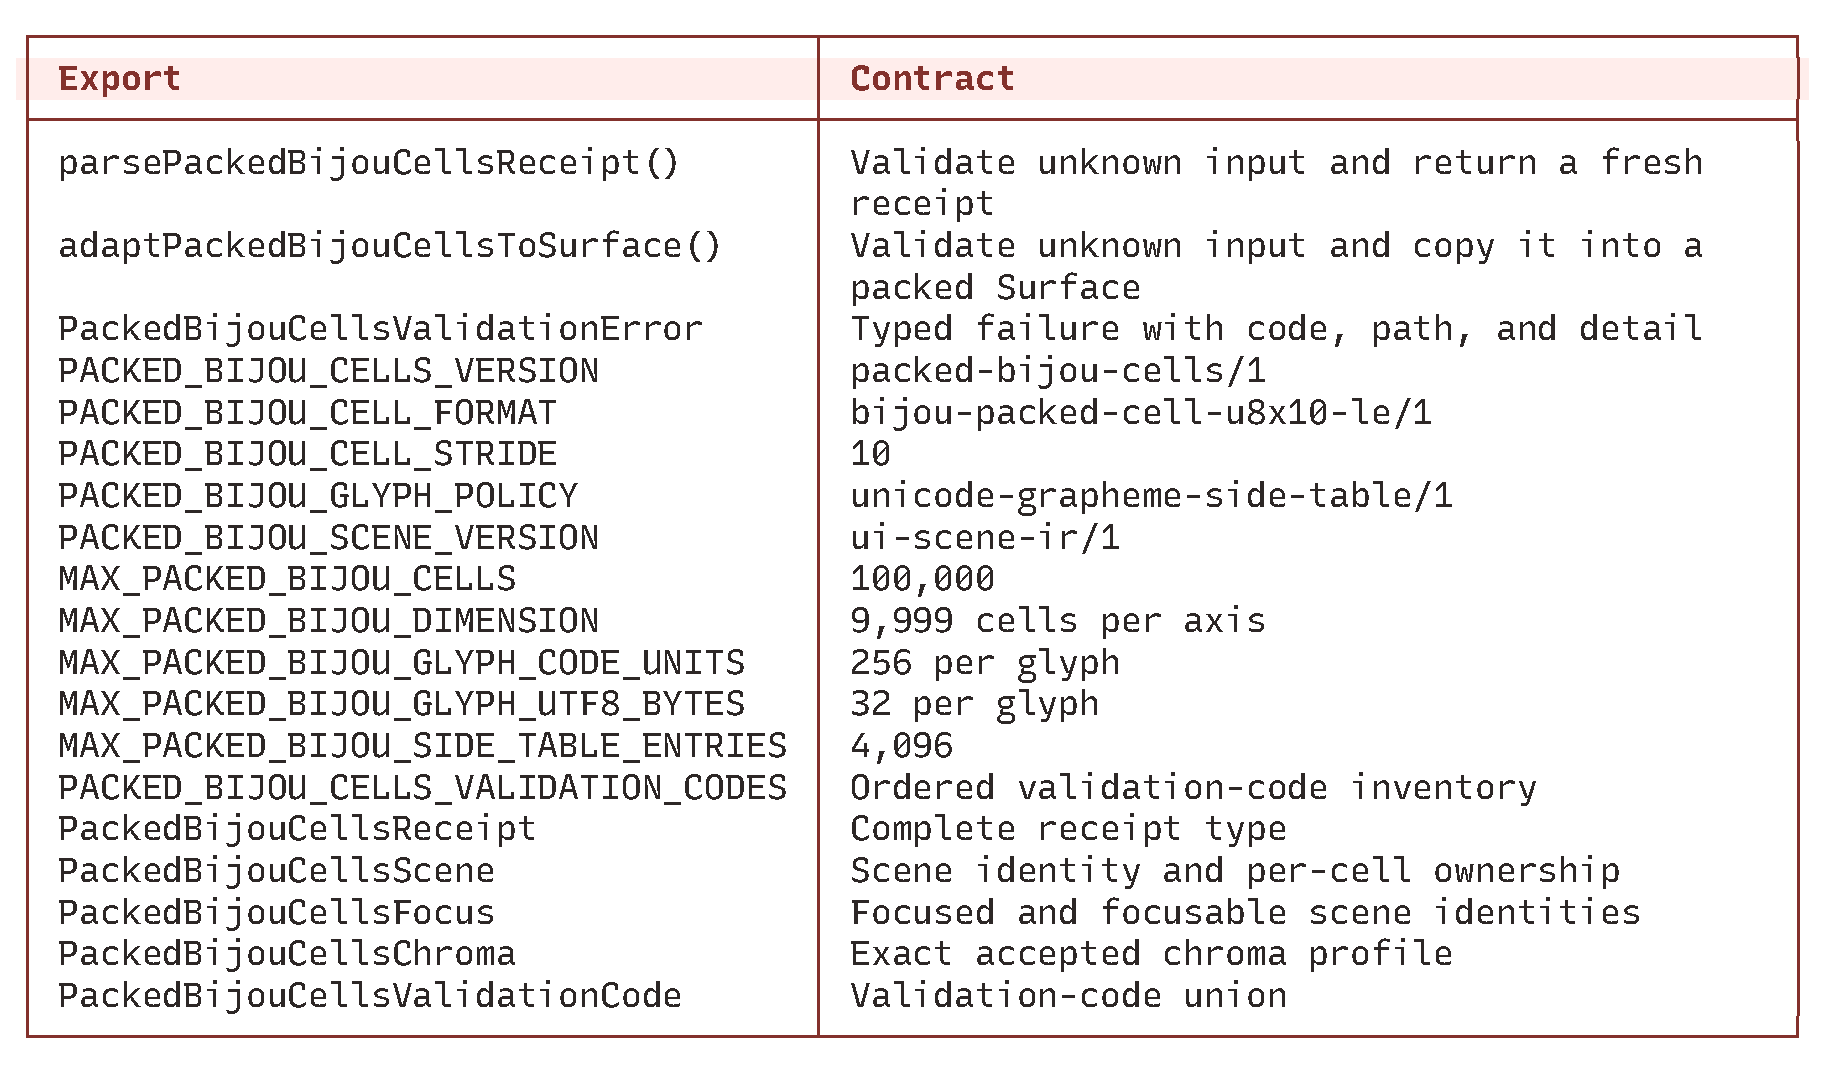
\includegraphics[width=\linewidth]{figures/tables/table-009-g1-1.pdf}
\par\smallskip{\scriptsize\color{BookMuted}Rows 1–19. Actual Bijou table component.}
\end{center}


Import the functions and receipt type from \texttt{@\allowbreak{}f\allowbreak{}l\allowbreak{}y\allowbreak{}i\allowbreak{}n\allowbreak{}g\allowbreak{}r\allowbreak{}o\allowbreak{}b\allowbreak{}o\allowbreak{}t\allowbreak{}s\allowbreak{}/\allowbreak{}b\allowbreak{}i\allowbreak{}j\allowbreak{}o\allowbreak{}u}:

\begin{CodeBlock}
import {
  adaptPackedBijouCellsToSurface,
  parsePackedBijouCellsReceipt,
  type PackedBijouCellsReceipt,
} from '@flyingrobots/bijou';
\end{CodeBlock}

Validate unknown input without constructing a \texttt{S\allowbreak{}u\allowbreak{}r\allowbreak{}f\allowbreak{}a\allowbreak{}c\allowbreak{}e}:

\begin{CodeBlock}
export function validateReceipt(
  input: unknown,
): PackedBijouCellsReceipt {
  return parsePackedBijouCellsReceipt(input);
}
\end{CodeBlock}

Adapt unknown input after validation:

\begin{CodeBlock}
export function adaptReceipt(input: unknown) {
  return adaptPackedBijouCellsToSurface(input);
}
\end{CodeBlock}

Both functions reject invalid input with \texttt{P\allowbreak{}a\allowbreak{}c\allowbreak{}k\allowbreak{}e\allowbreak{}d\allowbreak{}B\allowbreak{}i\allowbreak{}j\allowbreak{}o\allowbreak{}u\allowbreak{}C\allowbreak{}e\allowbreak{}l\allowbreak{}l\allowbreak{}s\allowbreak{}V\allowbreak{}a\allowbreak{}l\allowbreak{}i\allowbreak{}d\allowbreak{}a\allowbreak{}t\allowbreak{}i\allowbreak{}o\allowbreak{}n\allowbreak{}E\allowbreak{}r\allowbreak{}r\allowbreak{}o\allowbreak{}r}. Inspect its \texttt{c\allowbreak{}o\allowbreak{}d\allowbreak{}e}, \texttt{p\allowbreak{}a\allowbreak{}t\allowbreak{}h}, and \texttt{d\allowbreak{}e\allowbreak{}t\allowbreak{}a\allowbreak{}i\allowbreak{}l} fields instead of parsing the message.

\section{Receipt Shape}\label{record-022-receipt-shape}

Every field is required. Unknown or non-enumerable fields, accessors, symbols, sparse arrays, and non-JSON-shaped objects are rejected.

\begin{CodeBlock}
interface PackedBijouCellsReceipt {
  readonly receiptVersion: 'packed-bijou-cells/1';
  readonly widthCells: number;
  readonly heightCells: number;
  readonly cellFormatId: 'bijou-packed-cell-u8x10-le/1';
  readonly glyphPolicyId: 'unicode-grapheme-side-table/1';
  readonly bytes: readonly number[];
  readonly sideTable: readonly string[];
  readonly scene: {
    readonly sceneVersion: 'ui-scene-ir/1';
    readonly sceneHash: string;
    readonly nodeIds: readonly string[];
    readonly cellNodeIds: readonly string[];
  };
  readonly focus: {
    readonly focusedNodeId: string | null;
    readonly focusableNodeIds: readonly string[];
  };
  readonly chroma: {
    readonly colorSpace: 'srgb';
    readonly channelEncoding: 'uint8';
    readonly alphaEncoding: 'uint6';
    readonly terminalDefaultEncoding: 'presence-bits';
  };
}
\end{CodeBlock}

The maximum accepted receipt contains \texttt{1\allowbreak{}0\allowbreak{}0\allowbreak{},\allowbreak{}0\allowbreak{}0\allowbreak{}0} cells, with no axis longer than \texttt{9\allowbreak{},\allowbreak{}9\allowbreak{}9\allowbreak{}9} cells. The byte payload must contain exactly ten unsigned bytes per cell. Negative zero is not a canonical unsigned byte and is rejected.

\section{Cell And Glyph Rules}\label{record-022-cell-and-glyph-rules}

\texttt{c\allowbreak{}e\allowbreak{}l\allowbreak{}l\allowbreak{}F\allowbreak{}o\allowbreak{}r\allowbreak{}m\allowbreak{}a\allowbreak{}t\allowbreak{}I\allowbreak{}d} fixes each cell at ten bytes:

\begin{center}
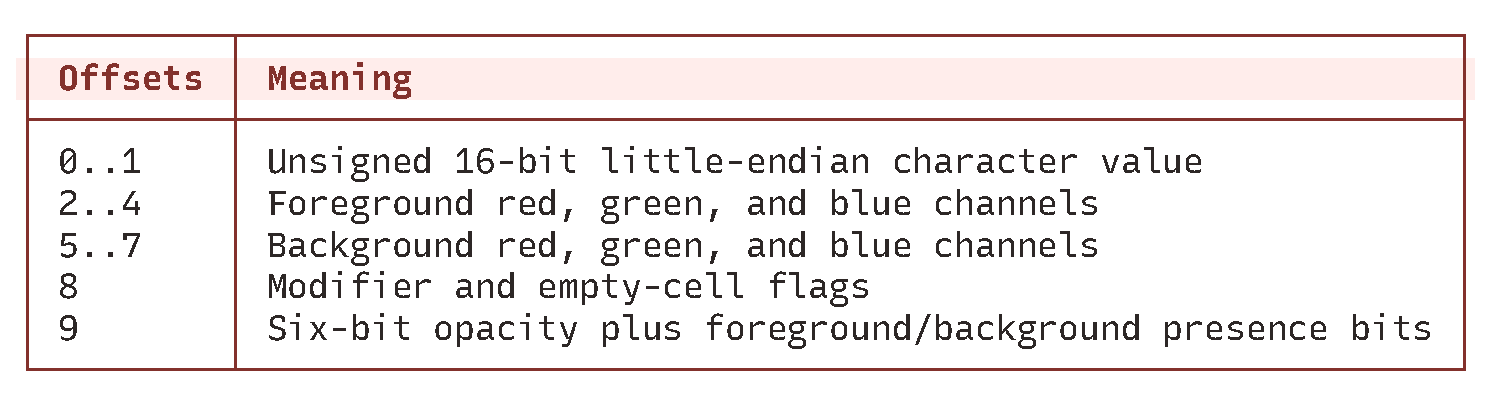
\includegraphics[width=\linewidth]{figures/tables/table-010-g1-1.pdf}
\par\smallskip{\scriptsize\color{BookMuted}Rows 1–5. Actual Bijou table component.}
\end{center}


Character values below \texttt{0\allowbreak{}x\allowbreak{}F\allowbreak{}0\allowbreak{}0\allowbreak{}0} are direct Basic Multilingual Plane values. Direct values must be terminal-control safe and have terminal width \texttt{1}; UTF-16 surrogate values and the NUL sentinel are rejected. An empty cell uses a space glyph plus the empty-cell flag. Values at or above \texttt{0\allowbreak{}x\allowbreak{}F\allowbreak{}0\allowbreak{}0\allowbreak{}0} select \texttt{s\allowbreak{}i\allowbreak{}d\allowbreak{}e\allowbreak{}T\allowbreak{}a\allowbreak{}b\allowbreak{}l\allowbreak{}e\allowbreak{}[\allowbreak{}c\allowbreak{}h\allowbreak{}a\allowbreak{}r\allowbreak{}a\allowbreak{}c\allowbreak{}t\allowbreak{}e\allowbreak{}r\allowbreak{}V\allowbreak{}a\allowbreak{}l\allowbreak{}u\allowbreak{}e\allowbreak{} \allowbreak{}-\allowbreak{} \allowbreak{}0\allowbreak{}x\allowbreak{}F\allowbreak{}0\allowbreak{}0\allowbreak{}0\allowbreak{}]}.

Each side-table entry must be unique, terminal-control safe, and exactly one grapheme with terminal width \texttt{1}. An entry contains at most \texttt{2\allowbreak{}5\allowbreak{}6} UTF-16 code units and encodes to at most \texttt{3\allowbreak{}2} UTF-8 bytes. Format-control, mark-only, and default-ignorable-only graphemes are rejected. Every entry must be referenced by at least one cell. A directly encodable value below \texttt{0\allowbreak{}x\allowbreak{}F\allowbreak{}0\allowbreak{}0\allowbreak{}0} is rejected from the side table. Side-table order is authoritative.

When a foreground or background presence bit is unset, the corresponding three color channels must be zero. An absent color means terminal default, not black. A dashed flag is valid only with the dotted/dashed underline bits.

\section{Scene, Focus, And Chroma Rules}\label{record-022-scene-focus-and-chroma-rules}

\texttt{s\allowbreak{}c\allowbreak{}e\allowbreak{}n\allowbreak{}e\allowbreak{}.\allowbreak{}s\allowbreak{}c\allowbreak{}e\allowbreak{}n\allowbreak{}e\allowbreak{}H\allowbreak{}a\allowbreak{}s\allowbreak{}h} is a lowercase SHA-256 hexadecimal digest. \texttt{s\allowbreak{}c\allowbreak{}e\allowbreak{}n\allowbreak{}e\allowbreak{}.\allowbreak{}n\allowbreak{}o\allowbreak{}d\allowbreak{}e\allowbreak{}I\allowbreak{}d\allowbreak{}s} is a unique non-empty inventory, and \texttt{s\allowbreak{}c\allowbreak{}e\allowbreak{}n\allowbreak{}e\allowbreak{}.\allowbreak{}c\allowbreak{}e\allowbreak{}l\allowbreak{}l\allowbreak{}N\allowbreak{}o\allowbreak{}d\allowbreak{}e\allowbreak{}I\allowbreak{}d\allowbreak{}s} contains one declared owner for every cell.

Every focusable node must occur in \texttt{s\allowbreak{}c\allowbreak{}e\allowbreak{}n\allowbreak{}e\allowbreak{}.\allowbreak{}n\allowbreak{}o\allowbreak{}d\allowbreak{}e\allowbreak{}I\allowbreak{}d\allowbreak{}s}. \texttt{f\allowbreak{}o\allowbreak{}c\allowbreak{}u\allowbreak{}s\allowbreak{}e\allowbreak{}d\allowbreak{}N\allowbreak{}o\allowbreak{}d\allowbreak{}e\allowbreak{}I\allowbreak{}d} is either \texttt{n\allowbreak{}u\allowbreak{}l\allowbreak{}l} or a member of \texttt{f\allowbreak{}o\allowbreak{}c\allowbreak{}u\allowbreak{}s\allowbreak{}a\allowbreak{}b\allowbreak{}l\allowbreak{}e\allowbreak{}N\allowbreak{}o\allowbreak{}d\allowbreak{}e\allowbreak{}I\allowbreak{}d\allowbreak{}s}.

Version \texttt{1} accepts only this chroma profile:

\begin{CodeBlock}
colorSpace: srgb
channelEncoding: uint8
alphaEncoding: uint6
terminalDefaultEncoding: presence-bits
\end{CodeBlock}

No color-space or channel conversion occurs.

\section{Diagnostics}\label{record-022-diagnostics}

The deterministic message format is:

\begin{CodeBlock}
packed-bijou-cells/1 <code> at <path>: <detail>
\end{CodeBlock}

Paths escape control and default-ignorable characters as Unicode escape sequences so diagnostics remain visually stable.

\begin{center}
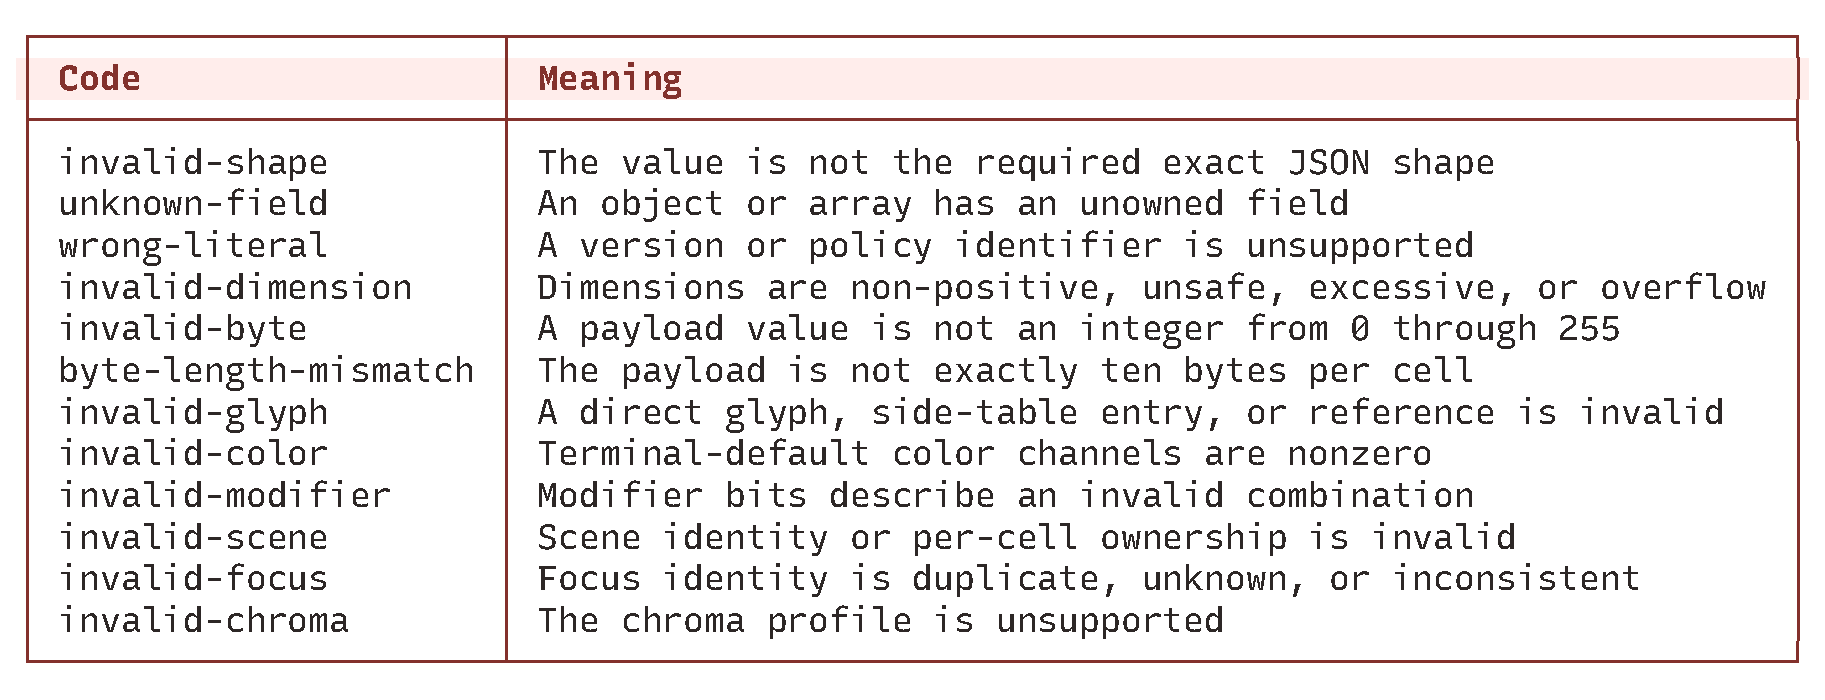
\includegraphics[width=\linewidth]{figures/tables/table-011-g1-1.pdf}
\par\smallskip{\scriptsize\color{BookMuted}Rows 1–12. Actual Bijou table component.}
\end{center}


Paths identify the rejected location, for example \texttt{\$\allowbreak{}.\allowbreak{}b\allowbreak{}y\allowbreak{}t\allowbreak{}e\allowbreak{}s\allowbreak{}[\allowbreak{}1\allowbreak{}7\allowbreak{}]} or \texttt{\$\allowbreak{}.\allowbreak{}f\allowbreak{}o\allowbreak{}c\allowbreak{}u\allowbreak{}s\allowbreak{}.\allowbreak{}f\allowbreak{}o\allowbreak{}c\allowbreak{}u\allowbreak{}s\allowbreak{}e\allowbreak{}d\allowbreak{}N\allowbreak{}o\allowbreak{}d\allowbreak{}e\allowbreak{}I\allowbreak{}d}.

\section{Adapter Result}\label{record-022-adapter-result}

\texttt{a\allowbreak{}d\allowbreak{}a\allowbreak{}p\allowbreak{}t\allowbreak{}P\allowbreak{}a\allowbreak{}c\allowbreak{}k\allowbreak{}e\allowbreak{}d\allowbreak{}B\allowbreak{}i\allowbreak{}j\allowbreak{}o\allowbreak{}u\allowbreak{}C\allowbreak{}e\allowbreak{}l\allowbreak{}l\allowbreak{}s\allowbreak{}T\allowbreak{}o\allowbreak{}S\allowbreak{}u\allowbreak{}r\allowbreak{}f\allowbreak{}a\allowbreak{}c\allowbreak{}e\allowbreak{}(\allowbreak{})} validates the complete receipt before it calls \texttt{c\allowbreak{}r\allowbreak{}e\allowbreak{}a\allowbreak{}t\allowbreak{}e\allowbreak{}S\allowbreak{}u\allowbreak{}r\allowbreak{}f\allowbreak{}a\allowbreak{}c\allowbreak{}e\allowbreak{}(\allowbreak{})}. On success:

\begin{CodeBlock}
surface.width === receipt.widthCells
surface.height === receipt.heightCells
Array.from(surface.buffer) deep-equals receipt.bytes
surface.sideTable deep-equals receipt.sideTable
\end{CodeBlock}

All surface cells are marked dirty for their first render. Scene, focus, and chroma metadata remain receipt evidence; they are not stored inside \texttt{S\allowbreak{}u\allowbreak{}r\allowbreak{}f\allowbreak{}a\allowbreak{}c\allowbreak{}e}.

\section{Fixture And Verification}\label{record-022-fixture-and-verification}

The checked fixture exercises direct glyphs, side-table glyphs, explicit and terminal-default colors, scene ownership, and focus:

\begin{itemize}
\tightlist
\item
  \href{https://github.com/flyingrobots/bijou/blob/cbd70612140e7a450d764b3c7be1c6af878b99bc/tests/fixtures/RE-036/packed-bijou-cells.v1.json}{Packed Bijou cell fixture}
\item
  \href{https://github.com/flyingrobots/bijou/blob/cbd70612140e7a450d764b3c7be1c6af878b99bc/docs/design/RE-036-packed-bijou-cells-surface-adapter.md}{RE-036 design record}
\end{itemize}

Run the focused contract evidence:

\begin{CodeBlock}
npx vitest run tests/cycles/RE-036
\end{CodeBlock}

%
\chapter{Patterns}\label{record-023}

\noindent{\footnotesize\color{BookMuted}\path{docs/design-system/patterns.md}\par}\smallskip

This document defines the recurring product patterns that Bijou should support consistently.

These are the decision frameworks behind the component families.

\section{0. Selection, focus, and rhythm}\label{record-023-selection-focus-and-rhythm}

\subsection{The pattern}\label{record-023-the-pattern}

Bijou should make it obvious:

\begin{itemize}
\tightlist
\item
  which item is currently selected
\item
  which region currently owns input
\item
  which copy is primary versus supporting
\item
  how dense content is meant to breathe
\end{itemize}

These decisions should not be improvised per surface.

\subsection{Canonical rules}\label{record-023-canonical-rules}

\subsubsection{Background fill means current selection}\label{record-023-background-fill-means-current-selection}

Use background fill to indicate the current selected row or item inside a collection.

Why:

\begin{itemize}
\tightlist
\item
  it reads immediately in dense TUIs
\item
  it does not depend on one tiny pointer glyph
\item
  it survives better than hue-only emphasis when terminals differ
\end{itemize}

Selection may also use supporting cues such as:

\begin{itemize}
\tightlist
\item
  a leading chevron
\item
  bold value text
\item
  a stronger border inside the selected row
\end{itemize}

But those are supporting cues. The canonical selected-item treatment is still background fill.

\subsubsection{Structural accent means active region}\label{record-023-structural-accent-means-active-region}

Use a structural accent such as a gutter, border emphasis, or region frame to show the active region.

Why:

\begin{itemize}
\tightlist
\item
  region focus and row selection are not the same thing
\item
  a pane can be active while its selected row changes
\item
  a selected row can exist inside an inactive region without stealing shell ownership
\end{itemize}

The accent should describe ownership of input, not merely visual importance.

\subsubsection{Visible controls are a promise}\label{record-023-visible-controls-are-a-promise}

Follow \href{https://github.com/flyingrobots/bijou/blob/cbd70612140e7a450d764b3c7be1c6af878b99bc/docs/invariants/visible-controls-are-a-promise.md}{Visible Controls Are a Promise}.

If a region is not active, its controls should not be advertised as though they will work.

When the shell owns focus, shell controls replace pane-local cues.

\subsubsection{One cell of padding matters}\label{record-023-one-cell-of-padding-matters}

Dense TUIs still need rhythm.

Canonical defaults:

\begin{itemize}
\tightlist
\item
  one cell of padding between content and region edges
\item
  one blank line between titled sections
\item
  one blank line between preference rows or similar stacked interactive rows when the surface can afford it
\end{itemize}

Do not cram labels, values, and descriptions together when one cell of space would make the surface easier to parse.

\subsubsection{Stack beneath the label before truncating}\label{record-023-stack-beneath-the-label-before-truncating}

When labels and values compete for the same horizontal space:

\begin{itemize}
\tightlist
\item
  wrap or stack first
\item
  reflow second
\item
  truncate only when the surface truly demands single-line identity
\end{itemize}

For settings and similar rows, values should stack beneath the label before truncating into ambiguity.

Marquee is an explicit overflow behavior for compact, focused single-line surfaces. It is not the default solution.

\subsubsection{Supporting copy should look supporting}\label{record-023-supporting-copy-should-look-supporting}

Descriptions, helper copy, and secondary explanation should look visibly quieter than primary actions and current values.

Use:

\begin{itemize}
\tightlist
\item
  muted tokens
\item
  dim modifiers when needed
\item
  more breathing room around primary actions than around support prose
\end{itemize}

Do not make supporting copy compete with what the user is supposed to act on now.

\subsubsection{Layers should behave like a stack}\label{record-023-layers-should-behave-like-a-stack}

When interactive layers overlap, they should behave in top-down order.

Canonical rules:

\begin{itemize}
\tightlist
\item
  the topmost layer owns input
\item
  the topmost layer owns the visible control hints
\item
  dismiss actions target the topmost dismissible layer first
\item
  underlying regions do not keep advertising controls while covered
\end{itemize}

This means a palette, drawer, or modal should not merely look on top. It should also be the source of truth for routing and footer/help copy.

\section{1. Status and feedback}\label{record-023-status-and-feedback}

\subsection{The pattern}\label{record-023-the-pattern-1}

Not all feedback should interrupt the user equally. Choose the least disruptive surface that still preserves the needed meaning.

\subsection{Escalation ladder}\label{record-023-escalation-ladder}

\subsubsection{\texorpdfstring{\texttt{b\allowbreak{}a\allowbreak{}d\allowbreak{}g\allowbreak{}e\allowbreak{}(\allowbreak{})}}{}}\label{record-023-badge}

Use when:

\begin{itemize}
\tightlist
\item
  the status is compact
\item
  it belongs inline with another object
\item
  the surrounding content already provides context
\end{itemize}

Avoid when:

\begin{itemize}
\tightlist
\item
  the user must act on the information
\item
  the message needs explanation
\item
  the status must persist as its own block
\end{itemize}

\subsubsection{\texorpdfstring{\texttt{n\allowbreak{}o\allowbreak{}t\allowbreak{}e\allowbreak{}(\allowbreak{})}}{}}\label{record-023-note}

Use when:

\begin{itemize}
\tightlist
\item
  the user needs supporting explanation
\item
  the content is informational, not urgent
\item
  the message belongs inside a form or guided flow
\end{itemize}

Avoid when:

\begin{itemize}
\tightlist
\item
  urgency or danger must be communicated
\item
  the message should interrupt
\end{itemize}

\subsubsection{\texorpdfstring{\texttt{a\allowbreak{}l\allowbreak{}e\allowbreak{}r\allowbreak{}t\allowbreak{}(\allowbreak{})}}{}}\label{record-023-alert}

Use when:

\begin{itemize}
\tightlist
\item
  the state should remain in the document flow
\item
  the message is important enough to deserve its own block
\item
  the user should see it while reading or editing nearby content
\end{itemize}

Avoid when:

\begin{itemize}
\tightlist
\item
  the event is brief and transient
\item
  it belongs in an activity stream
\item
  the app should manage stack/history/lifecycle
\end{itemize}

\subsubsection{\texorpdfstring{\texttt{t\allowbreak{}o\allowbreak{}a\allowbreak{}s\allowbreak{}t\allowbreak{}(\allowbreak{})}}{}}\label{record-023-toast}

Use when:

\begin{itemize}
\tightlist
\item
  the event is transient
\item
  the app is composing a one-off overlay directly
\item
  custom placement matters, but full notification lifecycle does not
\end{itemize}

Avoid when:

\begin{itemize}
\tightlist
\item
  the message must remain in the page content
\item
  the app needs stacking, history, routing, or recall
\item
  the user needs to review a set of related events later
\end{itemize}

Content guidance:

\begin{itemize}
\tightlist
\item
  keep the message short and self-contained
\item
  do not hide follow-up obligations in a toast body
\item
  prefer one clear state statement over mixed status plus instructions plus history
\end{itemize}

\subsubsection{notifications}\label{record-023-notifications}

Use when:

\begin{itemize}
\tightlist
\item
  the app owns transient messaging as a system
\item
  stacking, placement, actions, routing, or history matter
\item
  the user may need to reopen or review prior notices
\end{itemize}

Avoid when:

\begin{itemize}
\tightlist
\item
  the message should remain in page content
\item
  a single local overlay would do
\item
  the user must stop and decide before continuing
\end{itemize}

Content guidance:

\begin{itemize}
\tightlist
\item
  use notifications for events, not for durable documents
\item
  route warnings and errors here when the app owns runtime messaging as a system
\item
  actionable notifications should expose one obvious next step, not a mini workflow
\item
  if users may need recall, the history/archive surface is part of the feature, not an optional afterthought
\end{itemize}

\subsubsection{\texorpdfstring{\texttt{m\allowbreak{}o\allowbreak{}d\allowbreak{}a\allowbreak{}l\allowbreak{}(\allowbreak{})}}{}}\label{record-023-modal}

Use when:

\begin{itemize}
\tightlist
\item
  the user must stop and decide
\item
  the app needs an explicit review or confirmation surface
\item
  background actions should be blocked
\end{itemize}

Avoid when:

\begin{itemize}
\tightlist
\item
  a lighter inline or overlay treatment would do
\end{itemize}

Content guidance:

\begin{itemize}
\tightlist
\item
  the title should state the decision or review task clearly
\item
  the body should explain the consequence, not repeat generic warning copy
\item
  the modal should end in a clear next action or dismissal path
\item
  avoid turning a modal into a drawer with extra blocking chrome
\end{itemize}

\subsubsection{\texorpdfstring{\texttt{s\allowbreak{}k\allowbreak{}e\allowbreak{}l\allowbreak{}e\allowbreak{}t\allowbreak{}o\allowbreak{}n\allowbreak{}(\allowbreak{})}}{}}\label{record-023-skeleton}

Use when:

\begin{itemize}
\tightlist
\item
  the content shape is known but a short-lived loading gap would otherwise cause layout pop
\item
  the user benefits from seeing where content will land
\end{itemize}

Avoid when:

\begin{itemize}
\tightlist
\item
  honest partial content is already available
\item
  the loading state is long-lived enough that explicit progress or retry messaging would be more honest
\item
  the placeholder would imply certainty the app does not actually have yet
\end{itemize}

\subsubsection{\texorpdfstring{\texttt{p\allowbreak{}r\allowbreak{}o\allowbreak{}g\allowbreak{}r\allowbreak{}e\allowbreak{}s\allowbreak{}s\allowbreak{}B\allowbreak{}a\allowbreak{}r\allowbreak{}(\allowbreak{})} / \texttt{c\allowbreak{}r\allowbreak{}e\allowbreak{}a\allowbreak{}t\allowbreak{}e\allowbreak{}A\allowbreak{}n\allowbreak{}i\allowbreak{}m\allowbreak{}a\allowbreak{}t\allowbreak{}e\allowbreak{}d\allowbreak{}P\allowbreak{}r\allowbreak{}o\allowbreak{}g\allowbreak{}r\allowbreak{}e\allowbreak{}s\allowbreak{}s\allowbreak{}B\allowbreak{}a\allowbreak{}r\allowbreak{}(\allowbreak{})}}{ / }}\label{record-023-progressbar-createanimatedprogressbar}

Use when:

\begin{itemize}
\tightlist
\item
  percent-complete is actually known or can be estimated honestly
\item
  the user benefits from determinate progress instead of generic activity
\end{itemize}

Avoid when:

\begin{itemize}
\tightlist
\item
  completion is unknown and the percentage would be fake
\item
  the work is so brief that the bar would only flicker
\end{itemize}

Loading-screen rule:

\begin{itemize}
\tightlist
\item
  a loading screen should show at most one progress bar
\item
  that bar must represent actual loading progress
\item
  do not use a progress bar on a title or splash screen unless the screen is truly a loading surface
\end{itemize}

\subsubsection{\texorpdfstring{\texttt{s\allowbreak{}p\allowbreak{}i\allowbreak{}n\allowbreak{}n\allowbreak{}e\allowbreak{}r\allowbreak{}F\allowbreak{}r\allowbreak{}a\allowbreak{}m\allowbreak{}e\allowbreak{}(\allowbreak{})} / \texttt{c\allowbreak{}r\allowbreak{}e\allowbreak{}a\allowbreak{}t\allowbreak{}e\allowbreak{}S\allowbreak{}p\allowbreak{}i\allowbreak{}n\allowbreak{}n\allowbreak{}e\allowbreak{}r\allowbreak{}(\allowbreak{})}}{ / }}\label{record-023-spinnerframe-createspinner}

Use when:

\begin{itemize}
\tightlist
\item
  the task is active but indeterminate
\item
  the user needs reassurance that work is still happening
\end{itemize}

Avoid when:

\begin{itemize}
\tightlist
\item
  completion can be expressed honestly as a determinate bar
\item
  animation would distract more than it reassures
\end{itemize}

\section{2. Selection versus action}\label{record-023-selection-versus-action}

This is one of the easiest places for a component library to become fuzzy.

\subsection{\texorpdfstring{\texttt{s\allowbreak{}e\allowbreak{}l\allowbreak{}e\allowbreak{}c\allowbreak{}t\allowbreak{}(\allowbreak{})}}{}}\label{record-023-select}

Use when:

\begin{itemize}
\tightlist
\item
  the user is choosing one value
\item
  the set is short and stable
\item
  the result becomes stored state
\end{itemize}

Avoid when:

\begin{itemize}
\tightlist
\item
  the list is large enough that search is the real task
\item
  the outcome should trigger an immediate app command instead of persisting a value
\end{itemize}

\subsection{\texorpdfstring{\texttt{m\allowbreak{}u\allowbreak{}l\allowbreak{}t\allowbreak{}i\allowbreak{}s\allowbreak{}e\allowbreak{}l\allowbreak{}e\allowbreak{}c\allowbreak{}t\allowbreak{}(\allowbreak{})}}{}}\label{record-023-multiselect}

Use when:

\begin{itemize}
\tightlist
\item
  the user is building a set
\item
  multiple simultaneous selections are meaningful
\end{itemize}

Avoid when:

\begin{itemize}
\tightlist
\item
  the user should choose exactly one option
\item
  the user is really firing commands one at a time instead of building a lasting set
\end{itemize}

\subsection{\texorpdfstring{\texttt{f\allowbreak{}i\allowbreak{}l\allowbreak{}t\allowbreak{}e\allowbreak{}r\allowbreak{}(\allowbreak{})}}{}}\label{record-023-filter}

Use when:

\begin{itemize}
\tightlist
\item
  the user is choosing one value from a larger set
\item
  search/narrowing is the main task
\end{itemize}

Avoid when:

\begin{itemize}
\tightlist
\item
  the option set is already short and stable enough for \texttt{s\allowbreak{}e\allowbreak{}l\allowbreak{}e\allowbreak{}c\allowbreak{}t\allowbreak{}(\allowbreak{})}
\item
  the result is a command or navigation action rather than stored value state
\end{itemize}

\subsection{\texorpdfstring{\texttt{c\allowbreak{}o\allowbreak{}m\allowbreak{}m\allowbreak{}a\allowbreak{}n\allowbreak{}d\allowbreak{}P\allowbreak{}a\allowbreak{}l\allowbreak{}e\allowbreak{}t\allowbreak{}t\allowbreak{}e\allowbreak{}(\allowbreak{})} / \texttt{c\allowbreak{}o\allowbreak{}m\allowbreak{}m\allowbreak{}a\allowbreak{}n\allowbreak{}d\allowbreak{}P\allowbreak{}a\allowbreak{}l\allowbreak{}e\allowbreak{}t\allowbreak{}t\allowbreak{}e\allowbreak{}S\allowbreak{}u\allowbreak{}r\allowbreak{}f\allowbreak{}a\allowbreak{}c\allowbreak{}e\allowbreak{}(\allowbreak{})}}{ / }}\label{record-023-commandpalette-commandpalettesurface}

Use when:

\begin{itemize}
\tightlist
\item
  the result is an action, navigation, or command
\item
  the app wants one global action-discovery surface
\item
  the user may benefit from mixed command groups such as actions, navigation, or recent destinations
\end{itemize}

Content guidance:

\begin{itemize}
\tightlist
\item
  palette entries should read like things the app can do, not field values the app stores
\item
  group commands by user intent (\texttt{N\allowbreak{}a\allowbreak{}v\allowbreak{}i\allowbreak{}g\allowbreak{}a\allowbreak{}t\allowbreak{}i\allowbreak{}o\allowbreak{}n}, \texttt{A\allowbreak{}c\allowbreak{}t\allowbreak{}i\allowbreak{}o\allowbreak{}n\allowbreak{}s}, \texttt{R\allowbreak{}e\allowbreak{}c\allowbreak{}e\allowbreak{}n\allowbreak{}t}) instead of raw subsystem names when possible
\item
  keep descriptions short enough to scan without turning the palette into a browseable document
\end{itemize}

Avoid \texttt{c\allowbreak{}o\allowbreak{}m\allowbreak{}m\allowbreak{}a\allowbreak{}n\allowbreak{}d\allowbreak{}P\allowbreak{}a\allowbreak{}l\allowbreak{}e\allowbreak{}t\allowbreak{}t\allowbreak{}e\allowbreak{}(\allowbreak{})} / \texttt{c\allowbreak{}o\allowbreak{}m\allowbreak{}m\allowbreak{}a\allowbreak{}n\allowbreak{}d\allowbreak{}P\allowbreak{}a\allowbreak{}l\allowbreak{}e\allowbreak{}t\allowbreak{}t\allowbreak{}e\allowbreak{}S\allowbreak{}u\allowbreak{}r\allowbreak{}f\allowbreak{}a\allowbreak{}c\allowbreak{}e\allowbreak{}(\allowbreak{})} when:

\begin{itemize}
\tightlist
\item
  the user is filling out a field value
\item
  the result should behave like stored form data
\item
  the content is really a browseable record list rather than an action list
\end{itemize}

\section{3. Comparison versus browsing versus inspection}\label{record-023-comparison-versus-browsing-versus-inspection}

\subsection{\texorpdfstring{\texttt{t\allowbreak{}a\allowbreak{}b\allowbreak{}l\allowbreak{}e\allowbreak{}(\allowbreak{})}}{}}\label{record-023-table}

Use when:

\begin{itemize}
\tightlist
\item
  the user needs comparison across columns
\item
  the same attributes matter across many rows
\item
  the table should fit the available terminal width and wrap long cells instead of forcing callers to pre-compute column widths
\end{itemize}

Avoid when:

\begin{itemize}
\tightlist
\item
  hierarchy is the main point
\item
  the user needs focused keyboard inspection rather than passive comparison
\item
  the item set is effectively one-dimensional and would read more honestly as a list
\end{itemize}

Variants:

\begin{itemize}
\tightlist
\item
  \texttt{v\allowbreak{}a\allowbreak{}r\allowbreak{}i\allowbreak{}a\allowbreak{}n\allowbreak{}t\allowbreak{}:\allowbreak{} \allowbreak{}"\allowbreak{}b\allowbreak{}o\allowbreak{}x\allowbreak{}"} keeps the default Unicode boxed table
\item
  \texttt{v\allowbreak{}a\allowbreak{}r\allowbreak{}i\allowbreak{}a\allowbreak{}n\allowbreak{}t\allowbreak{}:\allowbreak{} \allowbreak{}"\allowbreak{}a\allowbreak{}s\allowbreak{}c\allowbreak{}i\allowbreak{}i\allowbreak{}-\allowbreak{}g\allowbreak{}r\allowbreak{}i\allowbreak{}d\allowbreak{}"} renders a portable \texttt{+\allowbreak{}-\allowbreak{}-\allowbreak{}-\allowbreak{}+} grid
\item
  \texttt{v\allowbreak{}a\allowbreak{}r\allowbreak{}i\allowbreak{}a\allowbreak{}n\allowbreak{}t\allowbreak{}:\allowbreak{} \allowbreak{}"\allowbreak{}r\allowbreak{}u\allowbreak{}l\allowbreak{}e\allowbreak{}d\allowbreak{}"} renders a borderless table with a heavy header rule and light row separators
\item
  \texttt{v\allowbreak{}a\allowbreak{}r\allowbreak{}i\allowbreak{}a\allowbreak{}n\allowbreak{}t\allowbreak{}:\allowbreak{} \allowbreak{}"\allowbreak{}h\allowbreak{}e\allowbreak{}a\allowbreak{}d\allowbreak{}e\allowbreak{}r\allowbreak{}-\allowbreak{}r\allowbreak{}u\allowbreak{}l\allowbreak{}e\allowbreak{}"} keeps only the header separator
\item
  \texttt{v\allowbreak{}a\allowbreak{}r\allowbreak{}i\allowbreak{}a\allowbreak{}n\allowbreak{}t\allowbreak{}:\allowbreak{} \allowbreak{}"\allowbreak{}p\allowbreak{}l\allowbreak{}a\allowbreak{}i\allowbreak{}n\allowbreak{}"} renders aligned columns with spaces and no rules
\item
  \texttt{v\allowbreak{}a\allowbreak{}r\allowbreak{}i\allowbreak{}a\allowbreak{}n\allowbreak{}t\allowbreak{}:\allowbreak{} \allowbreak{}"\allowbreak{}m\allowbreak{}a\allowbreak{}r\allowbreak{}k\allowbreak{}d\allowbreak{}o\allowbreak{}w\allowbreak{}n\allowbreak{}"} renders a GitHub-flavored Markdown pipe table
\item
  \texttt{v\allowbreak{}a\allowbreak{}r\allowbreak{}i\allowbreak{}a\allowbreak{}n\allowbreak{}t\allowbreak{}:\allowbreak{} \allowbreak{}"\allowbreak{}d\allowbreak{}e\allowbreak{}f\allowbreak{}i\allowbreak{}n\allowbreak{}i\allowbreak{}t\allowbreak{}i\allowbreak{}o\allowbreak{}n\allowbreak{}"} renders two-column field/value reports
\item
  \texttt{v\allowbreak{}a\allowbreak{}r\allowbreak{}i\allowbreak{}a\allowbreak{}n\allowbreak{}t\allowbreak{}:\allowbreak{} \allowbreak{}"\allowbreak{}e\allowbreak{}x\allowbreak{}p\allowbreak{}a\allowbreak{}n\allowbreak{}d\allowbreak{}e\allowbreak{}d\allowbreak{}"} renders psql-style record inspection
\end{itemize}

Examples:

\begin{CodeBlock}
box
┌───────┬────────┐
│ Name  │ State  │
├───────┼────────┤
│ Alice │ active │
└───────┴────────┘

ruled
Name   State
━━━━━  ━━━━━━
Alice  active

header-rule
Name   State
-----  ------
Alice  active

plain
Name   State
Alice  active

markdown
| Name  | State  |
|-------|--------|
| Alice | active |

definition
Field  Value
━━━━━  ━━━━━━
State  active

expanded
-[ RECORD 1 ]------------
Name  | Alice
State | active
\end{CodeBlock}

Lowering:

\begin{itemize}
\tightlist
\item
  \texttt{p\allowbreak{}i\allowbreak{}p\allowbreak{}e} mode still defaults to TSV
\item
  callers can opt into \texttt{p\allowbreak{}i\allowbreak{}p\allowbreak{}e\allowbreak{}F\allowbreak{}o\allowbreak{}r\allowbreak{}m\allowbreak{}a\allowbreak{}t\allowbreak{}:\allowbreak{} \allowbreak{}"\allowbreak{}c\allowbreak{}s\allowbreak{}v\allowbreak{}"}, \texttt{"\allowbreak{}m\allowbreak{}a\allowbreak{}r\allowbreak{}k\allowbreak{}d\allowbreak{}o\allowbreak{}w\allowbreak{}n\allowbreak{}"}, or \texttt{"\allowbreak{}a\allowbreak{}s\allowbreak{}c\allowbreak{}i\allowbreak{}i\allowbreak{}-\allowbreak{}g\allowbreak{}r\allowbreak{}i\allowbreak{}d\allowbreak{}"}
\item
  visual aligned-column variants use spaces, not tabs; tabs are reserved for TSV serialization
\end{itemize}

\subsection{\texorpdfstring{\texttt{t\allowbreak{}a\allowbreak{}b\allowbreak{}l\allowbreak{}e\allowbreak{}S\allowbreak{}u\allowbreak{}r\allowbreak{}f\allowbreak{}a\allowbreak{}c\allowbreak{}e\allowbreak{}(\allowbreak{})}}{}}\label{record-023-tablesurface}

Use when:

\begin{itemize}
\tightlist
\item
  the user needs the same passive comparison semantics as \texttt{t\allowbreak{}a\allowbreak{}b\allowbreak{}l\allowbreak{}e\allowbreak{}(\allowbreak{})}
\item
  the surrounding V3 runtime is already composing \texttt{S\allowbreak{}u\allowbreak{}r\allowbreak{}f\allowbreak{}a\allowbreak{}c\allowbreak{}e} output
\item
  cells may contain surface-native labels or badges
\end{itemize}

Avoid when:

\begin{itemize}
\tightlist
\item
  direct string output is the final destination
\item
  the app needs keyboard-owned row/cell focus semantics
\end{itemize}

\subsection{\texorpdfstring{\texttt{n\allowbreak{}a\allowbreak{}v\allowbreak{}i\allowbreak{}g\allowbreak{}a\allowbreak{}b\allowbreak{}l\allowbreak{}e\allowbreak{}T\allowbreak{}a\allowbreak{}b\allowbreak{}l\allowbreak{}e\allowbreak{}(\allowbreak{})} / \texttt{n\allowbreak{}a\allowbreak{}v\allowbreak{}i\allowbreak{}g\allowbreak{}a\allowbreak{}b\allowbreak{}l\allowbreak{}e\allowbreak{}T\allowbreak{}a\allowbreak{}b\allowbreak{}l\allowbreak{}e\allowbreak{}S\allowbreak{}u\allowbreak{}r\allowbreak{}f\allowbreak{}a\allowbreak{}c\allowbreak{}e\allowbreak{}(\allowbreak{})}}{ / }}\label{record-023-navigabletable-navigabletablesurface}

Use when:

\begin{itemize}
\tightlist
\item
  table data must be actively traversed
\item
  the app wants row/cell focus semantics
\item
  comparison across stable columns is still the job even while navigating
\end{itemize}

Avoid when:

\begin{itemize}
\tightlist
\item
  passive comparison is enough
\item
  the output must remain portable through core-only string rendering
\item
  the user is really selecting among one-dimensional records instead of comparing attributes
\end{itemize}

\subsection{\texorpdfstring{\texttt{b\allowbreak{}r\allowbreak{}o\allowbreak{}w\allowbreak{}s\allowbreak{}a\allowbreak{}b\allowbreak{}l\allowbreak{}e\allowbreak{}L\allowbreak{}i\allowbreak{}s\allowbreak{}t\allowbreak{}(\allowbreak{})} / \texttt{b\allowbreak{}r\allowbreak{}o\allowbreak{}w\allowbreak{}s\allowbreak{}a\allowbreak{}b\allowbreak{}l\allowbreak{}e\allowbreak{}L\allowbreak{}i\allowbreak{}s\allowbreak{}t\allowbreak{}S\allowbreak{}u\allowbreak{}r\allowbreak{}f\allowbreak{}a\allowbreak{}c\allowbreak{}e\allowbreak{}(\allowbreak{})}}{ / }}\label{record-023-browsablelist-browsablelistsurface}

Use when:

\begin{itemize}
\tightlist
\item
  items are one-dimensional
\item
  descriptions matter
\item
  the user is exploring or choosing among records
\end{itemize}

Avoid when:

\begin{itemize}
\tightlist
\item
  actions/commands are the result rather than records
\item
  column comparison is the point
\item
  hierarchy/path structure is the point
\end{itemize}

\subsection{\texorpdfstring{\texttt{f\allowbreak{}i\allowbreak{}l\allowbreak{}e\allowbreak{}P\allowbreak{}i\allowbreak{}c\allowbreak{}k\allowbreak{}e\allowbreak{}r\allowbreak{}(\allowbreak{})} / \texttt{f\allowbreak{}i\allowbreak{}l\allowbreak{}e\allowbreak{}P\allowbreak{}i\allowbreak{}c\allowbreak{}k\allowbreak{}e\allowbreak{}r\allowbreak{}S\allowbreak{}u\allowbreak{}r\allowbreak{}f\allowbreak{}a\allowbreak{}c\allowbreak{}e\allowbreak{}(\allowbreak{})}}{ / }}\label{record-023-filepicker-filepickersurface}

Use when:

\begin{itemize}
\tightlist
\item
  the user is traversing filesystem hierarchy
\item
  the current path and directory transitions are part of the job
\end{itemize}

Avoid when:

\begin{itemize}
\tightlist
\item
  the content is generic hierarchy rather than actual file/path navigation
\item
  actions/commands are the result rather than a selected file or directory
\end{itemize}

\section{3.5 Viewport masking and scroll ownership}\label{record-023-viewport-masking-and-scroll-ownership}

\subsection{Governing rules}\label{record-023-governing-rules}

\begin{itemize}
\tightlist
\item
  \texttt{v\allowbreak{}i\allowbreak{}e\allowbreak{}w\allowbreak{}p\allowbreak{}o\allowbreak{}r\allowbreak{}t\allowbreak{}S\allowbreak{}u\allowbreak{}r\allowbreak{}f\allowbreak{}a\allowbreak{}c\allowbreak{}e\allowbreak{}(\allowbreak{})} is the canonical masking primitive for bounded overflow scrolling in rich TUI composition.
\item
  \texttt{v\allowbreak{}i\allowbreak{}e\allowbreak{}w\allowbreak{}p\allowbreak{}o\allowbreak{}r\allowbreak{}t\allowbreak{}(\allowbreak{})} is the explicit text-lowering path when the content is intentionally string-first.
\item
  \texttt{p\allowbreak{}a\allowbreak{}g\allowbreak{}e\allowbreak{}r\allowbreak{}S\allowbreak{}u\allowbreak{}r\allowbreak{}f\allowbreak{}a\allowbreak{}c\allowbreak{}e\allowbreak{}(\allowbreak{})} and \texttt{f\allowbreak{}o\allowbreak{}c\allowbreak{}u\allowbreak{}s\allowbreak{}A\allowbreak{}r\allowbreak{}e\allowbreak{}a\allowbreak{}S\allowbreak{}u\allowbreak{}r\allowbreak{}f\allowbreak{}a\allowbreak{}c\allowbreak{}e\allowbreak{}(\allowbreak{})} are specialization layers on top of the viewport primitive, not separate scroll systems.
\item
  If a component only needs a clipped window plus scroll state, it should wrap viewport semantics rather than invent a bespoke \texttt{s\allowbreak{}c\allowbreak{}r\allowbreak{}o\allowbreak{}l\allowbreak{}l\allowbreak{}Y} slicer.
\item
  \texttt{n\allowbreak{}a\allowbreak{}v\allowbreak{}i\allowbreak{}g\allowbreak{}a\allowbreak{}b\allowbreak{}l\allowbreak{}e\allowbreak{}T\allowbreak{}a\allowbreak{}b\allowbreak{}l\allowbreak{}e\allowbreak{}S\allowbreak{}u\allowbreak{}r\allowbreak{}f\allowbreak{}a\allowbreak{}c\allowbreak{}e\allowbreak{}(\allowbreak{})} is the important exception: wrapped comparison rows keep row-aware scroll semantics, so generic line clipping is the wrong abstraction there.
\item
  Scroll ownership must stay unified. If keyboard focus, mouse hit-testing, and rendering disagree about the visible window height, the component has a layout bug.
\item
  Scrollbars belong to the viewport layer. Components should not fake overflow by moving rows around without giving the user a truthful masked window.
\end{itemize}

\subsection{Layout rules}\label{record-023-layout-rules}

\begin{itemize}
\tightlist
\item
  Components should either fill the rectangle their parent assigns them or be intentionally placed within it by a parent-owned layout helper such as \texttt{p\allowbreak{}l\allowbreak{}a\allowbreak{}c\allowbreak{}e\allowbreak{}S\allowbreak{}u\allowbreak{}r\allowbreak{}f\allowbreak{}a\allowbreak{}c\allowbreak{}e\allowbreak{}(\allowbreak{})}.
\item
  Parents own outer whitespace and anchoring. Child components should not silently shrink and leave accidental slack against a pane edge.
\item
  When a pane has a fixed header or separator row, the remaining rows should belong to one honest body region rather than an ad hoc mix of body plus invisible slack.
\item
  Overflow handling must be explicit: wrap, stack, clip, or viewport. Scrolling content without a matching viewport contract is not an acceptable fallback.
\end{itemize}

\subsection{\texorpdfstring{\texttt{v\allowbreak{}i\allowbreak{}e\allowbreak{}w\allowbreak{}p\allowbreak{}o\allowbreak{}r\allowbreak{}t\allowbreak{}S\allowbreak{}u\allowbreak{}r\allowbreak{}f\allowbreak{}a\allowbreak{}c\allowbreak{}e\allowbreak{}(\allowbreak{})}}{}}\label{record-023-viewportsurface}

Use when:

\begin{itemize}
\tightlist
\item
  an existing \texttt{S\allowbreak{}u\allowbreak{}r\allowbreak{}f\allowbreak{}a\allowbreak{}c\allowbreak{}e} or layout-backed region just needs a scrollable mask
\item
  the app already owns the surrounding chrome and only needs honest overflow scrolling
\item
  the component should stay on the structured \texttt{S\allowbreak{}u\allowbreak{}r\allowbreak{}f\allowbreak{}a\allowbreak{}c\allowbreak{}e} path
\end{itemize}

Avoid when:

\begin{itemize}
\tightlist
\item
  the content is intentionally string-first and the text-lowering path is the actual destination
\item
  the component needs domain-specific focus chrome or status semantics that belong in a higher-level wrapper
\end{itemize}

\section{3.6 Containment and formatted documents}\label{record-023-containment-and-formatted-documents}

\subsection{\texorpdfstring{\texttt{b\allowbreak{}o\allowbreak{}x\allowbreak{}(\allowbreak{})} / \texttt{h\allowbreak{}e\allowbreak{}a\allowbreak{}d\allowbreak{}e\allowbreak{}r\allowbreak{}B\allowbreak{}o\allowbreak{}x\allowbreak{}(\allowbreak{})}}{ / }}\label{record-023-box-headerbox}

Use when:

\begin{itemize}
\tightlist
\item
  a region needs visible containment or a local title
\item
  peer panels need to feel like separate working areas
\item
  compact metadata belongs in a header rather than in the surrounding prose
\end{itemize}

Avoid when:

\begin{itemize}
\tightlist
\item
  every subsection would get a border just for visual decoration
\item
  the real job is status escalation, not containment
\item
  a divider, heading, or simple whitespace would communicate structure more honestly
\end{itemize}

\subsection{\texorpdfstring{\texttt{m\allowbreak{}a\allowbreak{}r\allowbreak{}k\allowbreak{}d\allowbreak{}o\allowbreak{}w\allowbreak{}n\allowbreak{}(\allowbreak{})}}{}}\label{record-023-markdown}

Use when:

\begin{itemize}
\tightlist
\item
  the content is help, reference, release notes, or bounded prose
\item
  lightweight structure such as headings, lists, quotes, links, and code fences materially helps comprehension
\item
  the same content should lower honestly across rich, pipe, and accessible modes
\end{itemize}

Avoid when:

\begin{itemize}
\tightlist
\item
  the content is so large that it really needs document navigation instead of one rendered block
\item
  the prose is user-authored rich content that expects full browser-grade markdown semantics
\item
  the app is really laying out UI regions or controls and is trying to use markdown as a layout engine
\item
  dense comparison, forms, or command discovery are the real jobs
\end{itemize}

\subsection{\texorpdfstring{\texttt{h\allowbreak{}y\allowbreak{}p\allowbreak{}e\allowbreak{}r\allowbreak{}l\allowbreak{}i\allowbreak{}n\allowbreak{}k\allowbreak{}(\allowbreak{})}}{}}\label{record-023-hyperlink}

Use when:

\begin{itemize}
\tightlist
\item
  the destination itself should remain part of the rendered output
\item
  terminals with link support can benefit from clickability without hiding where the link goes
\end{itemize}

Avoid when:

\begin{itemize}
\tightlist
\item
  the label is vague or generic
\item
  trust depends on seeing the actual destination, but the surrounding content hides it
\item
  the interaction is really an app-owned action instead of an external destination
\end{itemize}

\subsection{\texorpdfstring{\texttt{k\allowbreak{}b\allowbreak{}d\allowbreak{}(\allowbreak{})}}{}}\label{record-023-kbd}

Use when:

\begin{itemize}
\tightlist
\item
  a local action needs an inline shortcut cue
\item
  the key hint belongs right next to the control, field, or instruction it affects
\end{itemize}

Avoid when:

\begin{itemize}
\tightlist
\item
  the user needs a grouped command reference or shell-level keymap
\item
  shortcut chips would start competing with the real content for attention
\end{itemize}

\subsection{\texorpdfstring{\texttt{p\allowbreak{}a\allowbreak{}g\allowbreak{}e\allowbreak{}r\allowbreak{}S\allowbreak{}u\allowbreak{}r\allowbreak{}f\allowbreak{}a\allowbreak{}c\allowbreak{}e\allowbreak{}(\allowbreak{})} / \texttt{f\allowbreak{}o\allowbreak{}c\allowbreak{}u\allowbreak{}s\allowbreak{}A\allowbreak{}r\allowbreak{}e\allowbreak{}a\allowbreak{}S\allowbreak{}u\allowbreak{}r\allowbreak{}f\allowbreak{}a\allowbreak{}c\allowbreak{}e\allowbreak{}(\allowbreak{})}}{ / }}\label{record-023-pagersurface-focusareasurface}

Use when:

\begin{itemize}
\tightlist
\item
  the scrollable region needs explicit line status, current-position framing, or focus gutter semantics
\item
  the pane is part of a larger workspace that needs visible ownership/focus signals
\end{itemize}

Avoid when:

\begin{itemize}
\tightlist
\item
  a plain masked region is enough and extra chrome would distract from the task
\end{itemize}

\subsection{Choosing among browseable structures}\label{record-023-choosing-among-browseable-structures}

\begin{itemize}
\tightlist
\item
  Choose \texttt{b\allowbreak{}r\allowbreak{}o\allowbreak{}w\allowbreak{}s\allowbreak{}a\allowbreak{}b\allowbreak{}l\allowbreak{}e\allowbreak{}L\allowbreak{}i\allowbreak{}s\allowbreak{}t\allowbreak{}S\allowbreak{}u\allowbreak{}r\allowbreak{}f\allowbreak{}a\allowbreak{}c\allowbreak{}e\allowbreak{}(\allowbreak{})} when rows are essentially labels plus brief descriptions.
\item
  Choose \texttt{c\allowbreak{}o\allowbreak{}m\allowbreak{}m\allowbreak{}a\allowbreak{}n\allowbreak{}d\allowbreak{}P\allowbreak{}a\allowbreak{}l\allowbreak{}e\allowbreak{}t\allowbreak{}t\allowbreak{}e\allowbreak{}S\allowbreak{}u\allowbreak{}r\allowbreak{}f\allowbreak{}a\allowbreak{}c\allowbreak{}e\allowbreak{}(\allowbreak{})} when the outcome is an action or navigation command.
\item
  Choose \texttt{f\allowbreak{}i\allowbreak{}l\allowbreak{}e\allowbreak{}P\allowbreak{}i\allowbreak{}c\allowbreak{}k\allowbreak{}e\allowbreak{}r\allowbreak{}S\allowbreak{}u\allowbreak{}r\allowbreak{}f\allowbreak{}a\allowbreak{}c\allowbreak{}e\allowbreak{}(\allowbreak{})} when path traversal is the mental model.
\item
  Choose \texttt{n\allowbreak{}a\allowbreak{}v\allowbreak{}i\allowbreak{}g\allowbreak{}a\allowbreak{}b\allowbreak{}l\allowbreak{}e\allowbreak{}T\allowbreak{}a\allowbreak{}b\allowbreak{}l\allowbreak{}e\allowbreak{}S\allowbreak{}u\allowbreak{}r\allowbreak{}f\allowbreak{}a\allowbreak{}c\allowbreak{}e\allowbreak{}(\allowbreak{})} when comparison across columns remains the job even while navigating.
\item
  Choose \texttt{v\allowbreak{}i\allowbreak{}e\allowbreak{}w\allowbreak{}p\allowbreak{}o\allowbreak{}r\allowbreak{}t\allowbreak{}S\allowbreak{}u\allowbreak{}r\allowbreak{}f\allowbreak{}a\allowbreak{}c\allowbreak{}e\allowbreak{}(\allowbreak{})} directly when the content already exists as a region and just needs bounded overflow masking.
\end{itemize}

\subsection{\texorpdfstring{\texttt{t\allowbreak{}r\allowbreak{}e\allowbreak{}e\allowbreak{}(\allowbreak{})}}{}}\label{record-023-tree}

Use when:

\begin{itemize}
\tightlist
\item
  the primary relationship is parent/child
\item
  the user needs to understand nesting or containment
\end{itemize}

Avoid when:

\begin{itemize}
\tightlist
\item
  multiple parents or dependency edges matter
\item
  the user is really traversing filesystem paths, where \texttt{f\allowbreak{}i\allowbreak{}l\allowbreak{}e\allowbreak{}P\allowbreak{}i\allowbreak{}c\allowbreak{}k\allowbreak{}e\allowbreak{}r\allowbreak{}S\allowbreak{}u\allowbreak{}r\allowbreak{}f\allowbreak{}a\allowbreak{}c\allowbreak{}e\allowbreak{}(\allowbreak{})} is more honest
\item
  dense row/column comparison would communicate the content more clearly than nesting
\end{itemize}

\subsection{\texorpdfstring{\texttt{d\allowbreak{}a\allowbreak{}g\allowbreak{}(\allowbreak{})} / \texttt{d\allowbreak{}a\allowbreak{}g\allowbreak{}P\allowbreak{}a\allowbreak{}n\allowbreak{}e\allowbreak{}(\allowbreak{})}}{ / }}\label{record-023-dag-dagpane}

Use when:

\begin{itemize}
\tightlist
\item
  the primary relationship is dependency or flow
\item
  multiple parents or graph edges matter
\item
  the user needs to answer questions like ``what does this depend on?'' or ``what does this unblock?''
\end{itemize}

Avoid when:

\begin{itemize}
\tightlist
\item
  a tree, timeline, or table would answer the question more directly
\item
  the graph would mostly act as architecture wallpaper instead of supporting a concrete task
\item
  the user really needs a metrics summary or focused fragment instead of the whole graph
\end{itemize}

\subsection{\texorpdfstring{\texttt{t\allowbreak{}i\allowbreak{}m\allowbreak{}e\allowbreak{}l\allowbreak{}i\allowbreak{}n\allowbreak{}e\allowbreak{}(\allowbreak{})}}{}}\label{record-023-timeline}

Use when:

\begin{itemize}
\tightlist
\item
  chronology is the main structure
\item
  events should read as a sequence, milestone trail, or audit-oriented progression
\end{itemize}

Avoid when:

\begin{itemize}
\tightlist
\item
  dependency or causality matters more than ordering
\item
  the content is so dense that a table, log, or summary-plus-detail drill-down would be more readable
\item
  the user is really comparing attributes across many events rather than following a temporal story
\end{itemize}

\section{3.7 Expressive branding and decorative emphasis}\label{record-023-expressive-branding-and-decorative-emphasis}

\subsection{\texorpdfstring{\texttt{l\allowbreak{}o\allowbreak{}a\allowbreak{}d\allowbreak{}R\allowbreak{}a\allowbreak{}n\allowbreak{}d\allowbreak{}o\allowbreak{}m\allowbreak{}L\allowbreak{}o\allowbreak{}g\allowbreak{}o\allowbreak{}(\allowbreak{})} / \texttt{g\allowbreak{}r\allowbreak{}a\allowbreak{}d\allowbreak{}i\allowbreak{}e\allowbreak{}n\allowbreak{}t\allowbreak{}T\allowbreak{}e\allowbreak{}x\allowbreak{}t\allowbreak{}(\allowbreak{})}}{ / }}\label{record-023-loadrandomlogo-gradienttext}

Use when:

\begin{itemize}
\tightlist
\item
  the product needs a deliberate branded or celebratory moment
\item
  splash surfaces, docs, or demos benefit from a little atmosphere
\end{itemize}

Avoid when:

\begin{itemize}
\tightlist
\item
  ordinary workspace chrome, navigation, status, or instructions need to stay neutral and legible
\item
  the emphasis would compete with the actual task
\item
  the color treatment is being asked to carry meaning that should live in text
\end{itemize}

\section{5. App-authored primitives}\label{record-023-app-authored-primitives}

\subsection{\texorpdfstring{\texttt{r\allowbreak{}e\allowbreak{}n\allowbreak{}d\allowbreak{}e\allowbreak{}r\allowbreak{}B\allowbreak{}y\allowbreak{}M\allowbreak{}o\allowbreak{}d\allowbreak{}e\allowbreak{}(\allowbreak{})}}{}}\label{record-023-renderbymode}

Use when:

\begin{itemize}
\tightlist
\item
  the app needs a domain-specific primitive that the shared component library should not own
\item
  the same semantic concept must lower honestly across rich, pipe, and accessible output
\end{itemize}

Avoid when:

\begin{itemize}
\tightlist
\item
  a shipped Bijou family already matches the job
\item
  the branching only exists to chase visual novelty instead of preserving meaning
\end{itemize}

\section{4. Disclosure and progressive complexity}\label{record-023-disclosure-and-progressive-complexity}

\subsection{\texorpdfstring{\texttt{a\allowbreak{}c\allowbreak{}c\allowbreak{}o\allowbreak{}r\allowbreak{}d\allowbreak{}i\allowbreak{}o\allowbreak{}n\allowbreak{}(\allowbreak{})}}{}}\label{record-023-accordion}

Use when:

\begin{itemize}
\tightlist
\item
  content is secondary or optional
\item
  one page can hold both summary and detail
\end{itemize}

Avoid when:

\begin{itemize}
\tightlist
\item
  the sections are peer destinations that deserve explicit navigation
\end{itemize}

\subsection{\texorpdfstring{\texttt{t\allowbreak{}a\allowbreak{}b\allowbreak{}s\allowbreak{}(\allowbreak{})}}{}}\label{record-023-tabs}

Use when:

\begin{itemize}
\tightlist
\item
  views are peers
\item
  only one view should be foregrounded at a time
\end{itemize}

Avoid when:

\begin{itemize}
\tightlist
\item
  the user is progressing through steps
\item
  hierarchy/path context matters more than peer switching
\end{itemize}

\subsection{\texorpdfstring{\texttt{s\allowbreak{}t\allowbreak{}e\allowbreak{}p\allowbreak{}p\allowbreak{}e\allowbreak{}r\allowbreak{}(\allowbreak{})}}{}}\label{record-023-stepper}

Use when:

\begin{itemize}
\tightlist
\item
  the user is moving through a process
\item
  order matters
\item
  the current stage should be understandable at a glance
\end{itemize}

Avoid when:

\begin{itemize}
\tightlist
\item
  the views are non-sequential
\item
  the user is really switching among peer destinations instead of progressing through a flow
\end{itemize}

\subsection{\texorpdfstring{\texttt{b\allowbreak{}r\allowbreak{}e\allowbreak{}a\allowbreak{}d\allowbreak{}c\allowbreak{}r\allowbreak{}u\allowbreak{}m\allowbreak{}b\allowbreak{}(\allowbreak{})}}{}}\label{record-023-breadcrumb}

Use when:

\begin{itemize}
\tightlist
\item
  the user needs path context
\item
  hierarchy or nesting should stay visible while reading the current location
\end{itemize}

Avoid when:

\begin{itemize}
\tightlist
\item
  peer destinations are the real model
\item
  the path is so deep or unstable that a simpler label plus local navigation would be clearer
\end{itemize}

\subsection{\texorpdfstring{\texttt{p\allowbreak{}a\allowbreak{}g\allowbreak{}i\allowbreak{}n\allowbreak{}a\allowbreak{}t\allowbreak{}o\allowbreak{}r\allowbreak{}(\allowbreak{})}}{}}\label{record-023-paginator}

Use when:

\begin{itemize}
\tightlist
\item
  the current page or position within a bounded sequence matters
\item
  page count should be visible without turning into a full navigation menu
\end{itemize}

Avoid when:

\begin{itemize}
\tightlist
\item
  the user needs rich peer navigation rather than compact progress
\item
  the content is an infinite feed or unbounded stream where page counts are misleading
\end{itemize}

\section{5. Overlay escalation}\label{record-023-overlay-escalation}

Choose overlays by how much they should interrupt and how much context they should retain.

\subsection{Governing rules}\label{record-023-governing-rules-1}

\begin{itemize}
\tightlist
\item
  Overlays are for interruption, review, or supplemental context. They are not substitutes for normal page structure.
\item
  Pick the least interruptive overlay that still preserves the meaning and action path.
\item
  If users need history, stacking, routing, or recall, move up from \texttt{t\allowbreak{}o\allowbreak{}a\allowbreak{}s\allowbreak{}t\allowbreak{}(\allowbreak{})} to the notification system.
\item
  If background input must stop, use \texttt{m\allowbreak{}o\allowbreak{}d\allowbreak{}a\allowbreak{}l\allowbreak{}(\allowbreak{})} rather than trying to make a toast or drawer behave like one.
\item
  If the content is long-lived and belongs in the reading flow, use \texttt{a\allowbreak{}l\allowbreak{}e\allowbreak{}r\allowbreak{}t\allowbreak{}(\allowbreak{})} or a normal page region instead of any overlay.
\item
  Use structured \texttt{S\allowbreak{}u\allowbreak{}r\allowbreak{}f\allowbreak{}a\allowbreak{}c\allowbreak{}e} content inside overlays when the interrupting layer needs real rows, embedded components, or richer layout. Flatten to plain text only at explicit lowering boundaries.
\end{itemize}

\subsection{\texorpdfstring{\texttt{t\allowbreak{}o\allowbreak{}o\allowbreak{}l\allowbreak{}t\allowbreak{}i\allowbreak{}p\allowbreak{}(\allowbreak{})}}{}}\label{record-023-tooltip}

\begin{itemize}
\tightlist
\item
  for tiny local explanation attached to nearby content
\item
  prefer one or two short lines that clarify a control, label, or state
\item
  not for decisions
\item
  not for content that needs scrolling, recall, commands, or workflow ownership
\end{itemize}

\subsection{\texorpdfstring{\texttt{d\allowbreak{}r\allowbreak{}a\allowbreak{}w\allowbreak{}e\allowbreak{}r\allowbreak{}(\allowbreak{})}}{}}\label{record-023-drawer}

\begin{itemize}
\tightlist
\item
  for supplemental context, inspectors, side work
\item
  keep the main surface visible
\item
  prefer when the user needs reference material while still working in the main task
\item
  use panel-scoped drawers when the supplemental context belongs to one workspace region instead of the whole frame
\item
  do not turn a drawer into a modal by stuffing it with blocking confirmation copy
\end{itemize}

\subsection{\texorpdfstring{\texttt{m\allowbreak{}o\allowbreak{}d\allowbreak{}a\allowbreak{}l\allowbreak{}(\allowbreak{})}}{}}\label{record-023-modal-1}

\begin{itemize}
\tightlist
\item
  for blocking review, choice, or confirmation
\item
  background shortcuts and pointer actions should be blocked
\item
  use sparingly; interruption must be justified
\item
  prefer short review-and-decide tasks over deep browsing or long-lived side work
\end{itemize}

\subsection{\texorpdfstring{\texttt{t\allowbreak{}o\allowbreak{}a\allowbreak{}s\allowbreak{}t\allowbreak{}(\allowbreak{})}}{}}\label{record-023-toast-1}

\begin{itemize}
\tightlist
\item
  for one transient overlay the app is composing directly
\item
  not for stack/history/routing problems
\item
  if the same class of event happens repeatedly, stop composing ad hoc toasts and move up to notifications
\end{itemize}

\subsection{notifications}\label{record-023-notifications-1}

\begin{itemize}
\tightlist
\item
  for events, not documents
\item
  use history/archive when recall matters
\item
  prefer over repeated ad hoc toasts once app-level messaging becomes systemic
\item
  route app-owned warnings and errors here when users may need to revisit them after the initial interruption
\item
  keep actions singular and obvious; do not hide multi-step workflows inside notification cards
\end{itemize}

\section{6. Forms and progression}\label{record-023-forms-and-progression}

\subsection{\texorpdfstring{\texttt{g\allowbreak{}r\allowbreak{}o\allowbreak{}u\allowbreak{}p\allowbreak{}(\allowbreak{})}}{}}\label{record-023-group}

Use when:

\begin{itemize}
\tightlist
\item
  the form fits one mental step
\item
  fields are directly related
\end{itemize}

\subsection{\texorpdfstring{\texttt{w\allowbreak{}i\allowbreak{}z\allowbreak{}a\allowbreak{}r\allowbreak{}d\allowbreak{}(\allowbreak{})}}{}}\label{record-023-wizard}

Use when:

\begin{itemize}
\tightlist
\item
  the flow has stages
\item
  branching or transformation matters
\item
  the user benefits from progressive disclosure
\end{itemize}

\subsection{\texorpdfstring{\texttt{c\allowbreak{}o\allowbreak{}n\allowbreak{}f\allowbreak{}i\allowbreak{}r\allowbreak{}m\allowbreak{}(\allowbreak{})}}{}}\label{record-023-confirm}

Use when:

\begin{itemize}
\tightlist
\item
  the decision is truly binary
\end{itemize}

Avoid when:

\begin{itemize}
\tightlist
\item
  the user needs to compare options or consequences in detail
\end{itemize}

\section{7. App shell composition}\label{record-023-app-shell-composition}

\subsection{Governing rules}\label{record-023-governing-rules-2}

\begin{itemize}
\tightlist
\item
  The shell exists to frame destinations, workspace state, and global actions. It should not compete with page content for narrative space.
\item
  Use shell chrome for orientation, status, and cross-cutting actions. Put explanation and task detail back into the page.
\item
  Prefer the simplest workspace that preserves the mental model. Do not use split panes or grids just because the runtime can.
\item
  If a region is not meaningfully inspectable, comparable, or supplemental, it probably should not be its own pane.
\item
  Keep shell roles distinct:

  \begin{itemize}
  \tightlist
  \item
    status rails communicate concise global state
  \item
    help hints teach shortcuts and scope
  \item
    command palette surfaces action discovery
  \item
    notifications surface events and follow-up
  \end{itemize}
\item
  If one shell element starts doing another shell element's job, the design is drifting.
\end{itemize}

\subsection{\texorpdfstring{\texttt{c\allowbreak{}r\allowbreak{}e\allowbreak{}a\allowbreak{}t\allowbreak{}e\allowbreak{}F\allowbreak{}r\allowbreak{}a\allowbreak{}m\allowbreak{}e\allowbreak{}d\allowbreak{}A\allowbreak{}p\allowbreak{}p\allowbreak{}(\allowbreak{})}}{}}\label{record-023-createframedapp}

Use when:

\begin{itemize}
\tightlist
\item
  the app has multiple views or work areas
\item
  shell chrome, palette, overlays, and notifications should be standardized
\item
  the frame should own the default hosted runtime path via \texttt{a\allowbreak{}p\allowbreak{}p\allowbreak{}.\allowbreak{}r\allowbreak{}u\allowbreak{}n\allowbreak{}(\allowbreak{}.\allowbreak{}.\allowbreak{}.\allowbreak{})} or \texttt{r\allowbreak{}u\allowbreak{}n\allowbreak{}F\allowbreak{}r\allowbreak{}a\allowbreak{}m\allowbreak{}e\allowbreak{}d\allowbreak{}A\allowbreak{}p\allowbreak{}p\allowbreak{}(\allowbreak{}.\allowbreak{}.\allowbreak{}.\allowbreak{})}
\end{itemize}

Avoid when:

\begin{itemize}
\tightlist
\item
  the app is really just one screen or one prompt loop
\end{itemize}

Content guidance:

\begin{itemize}
\tightlist
\item
  tabs should represent peer destinations, not unrelated commands
\item
  shell notifications and overlays should remain subordinate to the active page task
\item
  help text should clarify shell behavior, not restate page content
\item
  command palette entries should prefer actions and navigation targets, not field-style data entry or explanatory prose
\item
  use drawers for supplemental workspace context and notifications for event messaging; do not overload the status rail with either
\item
  prefer the self-running framed-shell path before dropping down to raw \texttt{r\allowbreak{}u\allowbreak{}n\allowbreak{}(\allowbreak{}a\allowbreak{}p\allowbreak{}p\allowbreak{})}
\end{itemize}

\subsection{\texorpdfstring{\texttt{s\allowbreak{}t\allowbreak{}a\allowbreak{}t\allowbreak{}u\allowbreak{}s\allowbreak{}B\allowbreak{}a\allowbreak{}r\allowbreak{}(\allowbreak{})} and \texttt{s\allowbreak{}t\allowbreak{}a\allowbreak{}t\allowbreak{}u\allowbreak{}s\allowbreak{}B\allowbreak{}a\allowbreak{}r\allowbreak{}S\allowbreak{}u\allowbreak{}r\allowbreak{}f\allowbreak{}a\allowbreak{}c\allowbreak{}e\allowbreak{}(\allowbreak{})}}{ and }}\label{record-023-statusbar-and-statusbarsurface}

Use when:

\begin{itemize}
\tightlist
\item
  global state, mode, or shortcut context belongs at the shell edge
\end{itemize}

Avoid when:

\begin{itemize}
\tightlist
\item
  the content is explanatory or multi-line
\end{itemize}

Content guidance:

\begin{itemize}
\tightlist
\item
  keep status text short, global, and low-drama
\item
  use \texttt{s\allowbreak{}t\allowbreak{}a\allowbreak{}t\allowbreak{}u\allowbreak{}s\allowbreak{}B\allowbreak{}a\allowbreak{}r\allowbreak{}S\allowbreak{}u\allowbreak{}r\allowbreak{}f\allowbreak{}a\allowbreak{}c\allowbreak{}e\allowbreak{}(\allowbreak{})} when shell chrome is already being composed as a \texttt{S\allowbreak{}u\allowbreak{}r\allowbreak{}f\allowbreak{}a\allowbreak{}c\allowbreak{}e}
\item
  keep \texttt{s\allowbreak{}t\allowbreak{}a\allowbreak{}t\allowbreak{}u\allowbreak{}s\allowbreak{}B\allowbreak{}a\allowbreak{}r\allowbreak{}(\allowbreak{})} for explicit text output or lowering
\item
  reserve strong emphasis for mode changes, faults, or focus-critical state
\item
  do not turn the status bar into a secondary page body
\item
  do not route transient warnings or task-specific explanation here when notifications or in-page content would be more honest
\end{itemize}

\subsection{\texorpdfstring{\texttt{h\allowbreak{}e\allowbreak{}l\allowbreak{}p\allowbreak{}S\allowbreak{}h\allowbreak{}o\allowbreak{}r\allowbreak{}t\allowbreak{}(\allowbreak{})} / \texttt{h\allowbreak{}e\allowbreak{}l\allowbreak{}p\allowbreak{}V\allowbreak{}i\allowbreak{}e\allowbreak{}w\allowbreak{}(\allowbreak{})} and surface companions}{ /  and surface companions}}\label{record-023-helpshort-helpview-and-surface-companions}

Use when:

\begin{itemize}
\tightlist
\item
  keyboard ownership is real and shortcut discovery needs a concise hint or grouped reference
\end{itemize}

Avoid when:

\begin{itemize}
\tightlist
\item
  the text would only restate visible controls without clarifying behavior or scope
\end{itemize}

Content guidance:

\begin{itemize}
\tightlist
\item
  use \texttt{h\allowbreak{}e\allowbreak{}l\allowbreak{}p\allowbreak{}S\allowbreak{}h\allowbreak{}o\allowbreak{}r\allowbreak{}t\allowbreak{}S\allowbreak{}u\allowbreak{}r\allowbreak{}f\allowbreak{}a\allowbreak{}c\allowbreak{}e\allowbreak{}(\allowbreak{})} for shell hints that stay on the structured \texttt{S\allowbreak{}u\allowbreak{}r\allowbreak{}f\allowbreak{}a\allowbreak{}c\allowbreak{}e} path
\item
  use \texttt{h\allowbreak{}e\allowbreak{}l\allowbreak{}p\allowbreak{}V\allowbreak{}i\allowbreak{}e\allowbreak{}w\allowbreak{}S\allowbreak{}u\allowbreak{}r\allowbreak{}f\allowbreak{}a\allowbreak{}c\allowbreak{}e\allowbreak{}(\allowbreak{})} for grouped shortcut references embedded inside a rich TUI surface or modal
\item
  keep the plain string helpers for explicit lowering, pipe output, or textual docs/examples
\item
  group by user intent (\texttt{N\allowbreak{}a\allowbreak{}v\allowbreak{}i\allowbreak{}g\allowbreak{}a\allowbreak{}t\allowbreak{}i\allowbreak{}o\allowbreak{}n}, \texttt{A\allowbreak{}c\allowbreak{}t\allowbreak{}i\allowbreak{}o\allowbreak{}n\allowbreak{}s}, \texttt{S\allowbreak{}e\allowbreak{}l\allowbreak{}e\allowbreak{}c\allowbreak{}t\allowbreak{}i\allowbreak{}o\allowbreak{}n}) rather than by key shape
\item
  help is for shortcut discovery and scope clarification, not for executing commands or replacing a command palette
\end{itemize}

\subsection{\texorpdfstring{\texttt{s\allowbreak{}p\allowbreak{}l\allowbreak{}i\allowbreak{}t\allowbreak{}P\allowbreak{}a\allowbreak{}n\allowbreak{}e\allowbreak{}(\allowbreak{})} and \texttt{g\allowbreak{}r\allowbreak{}i\allowbreak{}d\allowbreak{}(\allowbreak{})}}{ and }}\label{record-023-splitpane-and-grid}

Use when:

\begin{itemize}
\tightlist
\item
  spatial composition helps the user reason about the workspace
\end{itemize}

Avoid when:

\begin{itemize}
\tightlist
\item
  the layout would be simpler and more legible as a sequential flow
\end{itemize}

Content guidance:

\begin{itemize}
\tightlist
\item
  use split panes for comparison, side-by-side reference, or inspector-style secondary context
\item
  use grids when the user is reading across stable regions, not when one long column would be clearer
\item
  label regions by job, not by visual position alone
\end{itemize}

\section{8. Mouse and multimodal interaction}\label{record-023-mouse-and-multimodal-interaction}

Mouse support in Bijou should follow these rules:

\begin{itemize}
\tightlist
\item
  keyboard is baseline
\item
  mouse is enhancement
\item
  every click target should mirror an existing keyboard path
\item
  overlays consume pointer input before background content
\item
  drag is reserved for spatial interactions such as pane resizing
\end{itemize}

Good early mouse targets:

\begin{itemize}
\tightlist
\item
  tabs
\item
  split dividers
\item
  notification actions and dismiss buttons
\item
  list/table row focus
\end{itemize}

Bad early mouse targets:

\begin{itemize}
\tightlist
\item
  hover-only critical meaning
\item
  interactions that have no keyboard parity
\end{itemize}

\section{9. Lowering across modes}\label{record-023-lowering-across-modes}

Every pattern should have a graceful lowering story.

\subsection{Examples}\label{record-023-examples}

\section{10. Motion and shader effects}\label{record-023-motion-and-shader-effects}

Motion and shader effects are supporting patterns, not the product itself.

Use them when:

\begin{itemize}
\tightlist
\item
  they clarify transition, progress, focus, or spatial change
\item
  the user benefits from seeing continuity rather than a sudden visual jump
\item
  the effect reinforces the information architecture instead of competing with it
\end{itemize}

Avoid them when:

\begin{itemize}
\tightlist
\item
  they are only decorative noise
\item
  they make dense work harder to read
\item
  the same information would be clearer as stable content, a status change, or a simpler transition
\end{itemize}

Specific guidance:

\begin{itemize}
\item
  use transition shaders to reinforce page or workspace change, not to show off that the renderer can animate
\item
  use \texttt{c\allowbreak{}a\allowbreak{}n\allowbreak{}v\allowbreak{}a\allowbreak{}s\allowbreak{}(\allowbreak{})} for purposeful visual surfaces such as splash, background atmosphere, or dedicated visual moments, not as a default wrapper around ordinary productivity screens
\item
  reduced-motion and non-interactive modes must still tell the truth even when the effect disappears entirely
\item
  notifications may lower to logs or in-flow alerts
\item
  command palette may lower to documented shortcuts or static command lists
\item
  navigable inspection views may lower to passive read-only views
\item
  modals may lower to step-by-step prompts or inline confirmation blocks
\end{itemize}

The docs for each family should make that lowering explicit instead of assuming an interactive full-screen terminal.

%
\chapter{Pointer and Mouse Policy}\label{record-024}

\noindent{\footnotesize\color{BookMuted}\path{docs/design-system/pointer.md}\par}\smallskip

Bijou is keyboard-first, not keyboard-only.

Mouse support should improve fluency without creating a second product that only works for pointer users.

\section{What mouse is for}\label{record-024-what-mouse-is-for}

Use mouse in Bijou to:

\begin{itemize}
\tightlist
\item
  switch visible context quickly
\item
  dismiss or activate transient overlays
\item
  inspect and select already-visible objects
\item
  adjust obviously spatial controls such as split dividers
\end{itemize}

Do not use mouse as the only path to:

\begin{itemize}
\tightlist
\item
  submit forms
\item
  dismiss critical errors
\item
  navigate core app flows
\item
  reveal essential state through hover alone
\end{itemize}

\section{Routing order}\label{record-024-routing-order}

Pointer events should resolve from most interruptive layer to least:

\begin{enumerate}
\def\labelenumi{\arabic{enumi}.}
\tightlist
\item
  active modal or command surface
\item
  transient overlays and notifications
\item
  shell chrome
\item
  page content
\end{enumerate}

Background content should not keep receiving pointer actions while a true modal surface is open.

For shell and overlay families specifically:

\begin{itemize}
\tightlist
\item
  \texttt{m\allowbreak{}o\allowbreak{}d\allowbreak{}a\allowbreak{}l\allowbreak{}(\allowbreak{})} should consume pointer input ahead of everything behind it
\item
  notifications and ad hoc overlays should consume clicks before shell chrome or page content
\item
  shell tabs, palette rows, and pane-scoped overlay controls should behave like pointer shortcuts for already-available keyboard actions, not as pointer-exclusive product paths
\end{itemize}

\section{Click policy}\label{record-024-click-policy}

Clicks should usually mirror an existing keyboard action:

\begin{itemize}
\tightlist
\item
  clicking a tab should do what tab-switching already does
\item
  clicking a notification action should do what pressing \texttt{e\allowbreak{}n\allowbreak{}t\allowbreak{}e\allowbreak{}r} on the focused notification already does
\item
  clicking dismiss should do what the dismiss shortcut already does
\end{itemize}

If there is no keyboard-parity story, the pointer behavior is probably under-designed.

\section{Hover policy}\label{record-024-hover-policy}

Hover is optional and should never be the only carrier of important meaning.

Terminals vary widely in pointer fidelity, update rate, and user expectation. Hover can be useful for polish, but it is a weak foundation for essential workflows.

\section{Spatial policy}\label{record-024-spatial-policy}

Use drag only for controls that are already spatial by nature:

\begin{itemize}
\tightlist
\item
  split-pane dividers
\item
  canvas or graph inspection surfaces
\item
  future resizable inspectors or drawers
\end{itemize}

Avoid inventing drag gestures for ordinary list, table, or form interactions.

\section{Current library baseline}\label{record-024-current-library-baseline}

The current first-class mouse baseline in \texttt{@\allowbreak{}f\allowbreak{}l\allowbreak{}y\allowbreak{}i\allowbreak{}n\allowbreak{}g\allowbreak{}r\allowbreak{}o\allowbreak{}b\allowbreak{}o\allowbreak{}t\allowbreak{}s\allowbreak{}/\allowbreak{}b\allowbreak{}i\allowbreak{}j\allowbreak{}o\allowbreak{}u\allowbreak{}-\allowbreak{}t\allowbreak{}u\allowbreak{}i} should be:

\begin{itemize}
\tightlist
\item
  shell tabs are clickable
\item
  notification cards support click-to-dismiss and click-to-activate
\item
  mouse requires explicit runtime opt-in with \texttt{r\allowbreak{}u\allowbreak{}n\allowbreak{}(\allowbreak{}a\allowbreak{}p\allowbreak{}p\allowbreak{},\allowbreak{} \allowbreak{}\{\allowbreak{} \allowbreak{}m\allowbreak{}o\allowbreak{}u\allowbreak{}s\allowbreak{}e\allowbreak{}:\allowbreak{} \allowbreak{}t\allowbreak{}r\allowbreak{}u\allowbreak{}e\allowbreak{} \allowbreak{}\}\allowbreak{})}
\item
  modal-style overlays block background pointer interaction
\item
  shell/pane pointer routing should remain subordinate to overlay routing when interruptive surfaces are open
\end{itemize}

Further component adoption should follow the same rule:

\begin{itemize}
\tightlist
\item
  add mouse where it accelerates an existing interaction
\item
  keep keyboard parity
\item
  route overlays before background content
\end{itemize}

%
\chapter{Inspect Profunctor Page Artifacts}\label{record-025}

\noindent{\footnotesize\color{BookMuted}\path{docs/reference/profunctor-page-inspection.md}\par}\smallskip

Use \texttt{l\allowbreak{}o\allowbreak{}w\allowbreak{}e\allowbreak{}r\allowbreak{}P\allowbreak{}r\allowbreak{}o\allowbreak{}f\allowbreak{}u\allowbreak{}n\allowbreak{}c\allowbreak{}t\allowbreak{}o\allowbreak{}r\allowbreak{}P\allowbreak{}a\allowbreak{}g\allowbreak{}e\allowbreak{}A\allowbreak{}r\allowbreak{}t\allowbreak{}i\allowbreak{}f\allowbreak{}a\allowbreak{}c\allowbreak{}t\allowbreak{}s\allowbreak{}(\allowbreak{})} to validate and inspect one canonical Profunctor Page artifact family through Bijou's terminal target. The function returns a deterministic \texttt{u\allowbreak{}i\allowbreak{}-\allowbreak{}s\allowbreak{}c\allowbreak{}e\allowbreak{}n\allowbreak{}e\allowbreak{}-\allowbreak{}i\allowbreak{}r\allowbreak{}/\allowbreak{}1} scene, \texttt{S\allowbreak{}u\allowbreak{}r\allowbreak{}f\allowbreak{}a\allowbreak{}c\allowbreak{}e}, target map, receipt, and text witness. It does not mutate the input artifacts.

This reference covers the bounded \texttt{b\allowbreak{}i\allowbreak{}j\allowbreak{}o\allowbreak{}u\allowbreak{}-\allowbreak{}t\allowbreak{}e\allowbreak{}r\allowbreak{}m\allowbreak{}i\allowbreak{}n\allowbreak{}a\allowbreak{}l\allowbreak{}-\allowbreak{}p\allowbreak{}r\allowbreak{}o\allowbreak{}j\allowbreak{}e\allowbreak{}c\allowbreak{}t\allowbreak{}-\allowbreak{}p\allowbreak{}a\allowbreak{}g\allowbreak{}e\allowbreak{}/\allowbreak{}1} target. It is not a general Profunctor Page renderer.

\section{Public API}\label{record-025-public-api}

Import the function, error type, and input or output types from \texttt{@\allowbreak{}f\allowbreak{}l\allowbreak{}y\allowbreak{}i\allowbreak{}n\allowbreak{}g\allowbreak{}r\allowbreak{}o\allowbreak{}b\allowbreak{}o\allowbreak{}t\allowbreak{}s\allowbreak{}/\allowbreak{}b\allowbreak{}i\allowbreak{}j\allowbreak{}o\allowbreak{}u}:

\begin{CodeBlock}
import {
  lowerProfunctorPageArtifacts,
  ProfunctorPageTargetError,
  type ProfunctorArtifactInputs,
  type ProfunctorPageInspectionMode,
  type ProfunctorPageTargetProof,
} from '@flyingrobots/bijou';
\end{CodeBlock}

The call accepts three exact UTF-8 JSON sources:

\begin{CodeBlock}
const inputs: ProfunctorArtifactInputs = {
  page: {
    filename: 'page.profunctor.json',
    source: pageSource,
  },
  sourceMap: {
    filename: 'page.profunctor.map.json',
    source: sourceMapSource,
  },
  buildManifest: {
    filename: 'page.profunctor.build.json',
    source: buildManifestSource,
  },
};

const proof: ProfunctorPageTargetProof =
  lowerProfunctorPageArtifacts(inputs, { mode: 'source-refs' });
\end{CodeBlock}

The example is illustrative. \texttt{p\allowbreak{}a\allowbreak{}g\allowbreak{}e\allowbreak{}S\allowbreak{}o\allowbreak{}u\allowbreak{}r\allowbreak{}c\allowbreak{}e}, \texttt{s\allowbreak{}o\allowbreak{}u\allowbreak{}r\allowbreak{}c\allowbreak{}e\allowbreak{}M\allowbreak{}a\allowbreak{}p\allowbreak{}S\allowbreak{}o\allowbreak{}u\allowbreak{}r\allowbreak{}c\allowbreak{}e}, and \texttt{b\allowbreak{}u\allowbreak{}i\allowbreak{}l\allowbreak{}d\allowbreak{}M\allowbreak{}a\allowbreak{}n\allowbreak{}i\allowbreak{}f\allowbreak{}e\allowbreak{}s\allowbreak{}t\allowbreak{}S\allowbreak{}o\allowbreak{}u\allowbreak{}r\allowbreak{}c\allowbreak{}e} must contain the complete canonical artifact bytes.

\section{Inputs}\label{record-025-inputs}

\begin{center}
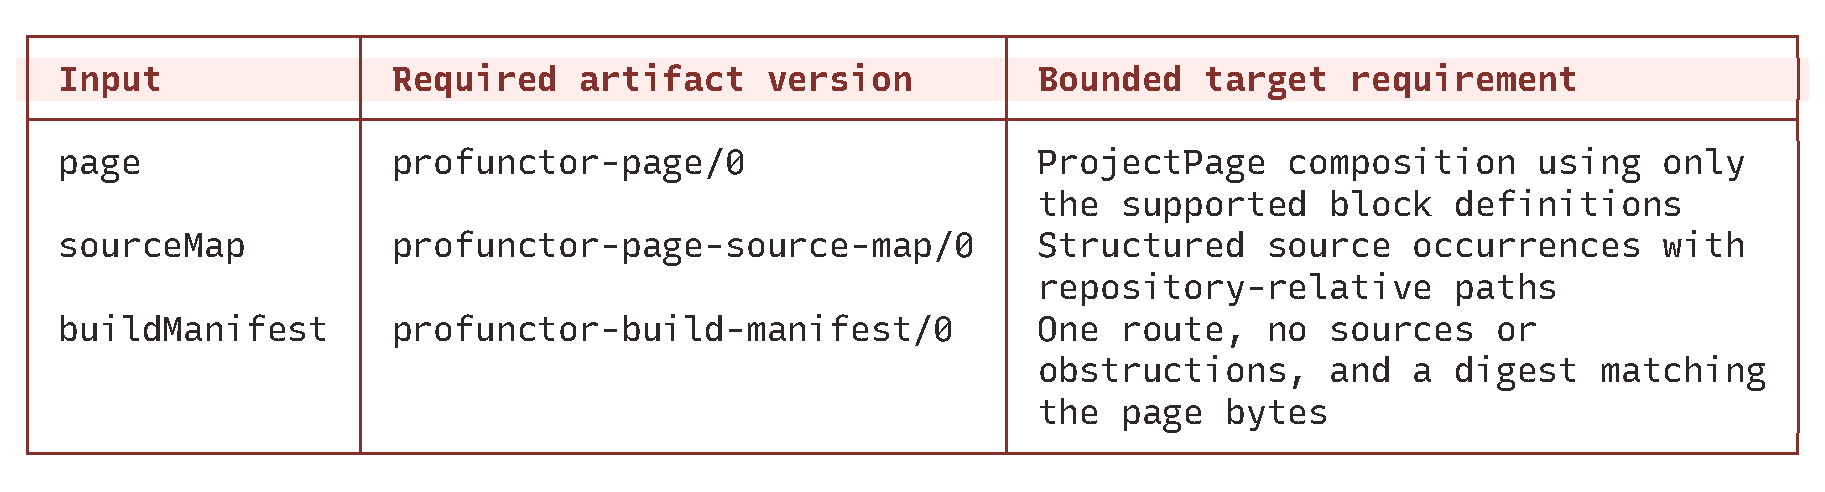
\includegraphics[width=\linewidth]{figures/tables/table-012-g1-1.pdf}
\par\smallskip{\scriptsize\color{BookMuted}Rows 1–3. Actual Bijou table component.}
\end{center}


Each source must be canonical JSON with either no trailing newline or exactly one trailing newline. The parser rejects unknown fields, missing fields, duplicate identities, malformed identity prefixes, host-local paths, digest drift, and cross-artifact disagreement.

The page, source map, and build manifest must agree on the page identity. The manifest entity must agree with the page entity, its sole route must equal the page route, and its dependencies must equal the page dependency digests in the same order. Every source-map source and record digest, node provenance source digest, and build entity digest must occur in that dependency list. The page root must be a visible \texttt{b\allowbreak{}l\allowbreak{}o\allowbreak{}c\allowbreak{}k\allowbreak{}:\allowbreak{}p\allowbreak{}a\allowbreak{}g\allowbreak{}e} whose route agrees with the page route. It must appear first in reading order, and every page node must be reachable from it through the declared slots.

\section{Supported Blocks}\label{record-025-supported-blocks}

The bounded target supports these visible block definitions:

\begin{itemize}
\tightlist
\item
  \texttt{b\allowbreak{}l\allowbreak{}o\allowbreak{}c\allowbreak{}k\allowbreak{}:\allowbreak{}p\allowbreak{}a\allowbreak{}g\allowbreak{}e}
\item
  \texttt{b\allowbreak{}l\allowbreak{}o\allowbreak{}c\allowbreak{}k\allowbreak{}:\allowbreak{}p\allowbreak{}r\allowbreak{}o\allowbreak{}j\allowbreak{}e\allowbreak{}c\allowbreak{}t\allowbreak{}-\allowbreak{}h\allowbreak{}e\allowbreak{}r\allowbreak{}o}
\item
  \texttt{b\allowbreak{}l\allowbreak{}o\allowbreak{}c\allowbreak{}k\allowbreak{}:\allowbreak{}p\allowbreak{}r\allowbreak{}o\allowbreak{}j\allowbreak{}e\allowbreak{}c\allowbreak{}t\allowbreak{}-\allowbreak{}f\allowbreak{}a\allowbreak{}c\allowbreak{}t\allowbreak{}s}
\item
  \texttt{b\allowbreak{}l\allowbreak{}o\allowbreak{}c\allowbreak{}k\allowbreak{}:\allowbreak{}p\allowbreak{}r\allowbreak{}o\allowbreak{}j\allowbreak{}e\allowbreak{}c\allowbreak{}t\allowbreak{}-\allowbreak{}d\allowbreak{}o\allowbreak{}c\allowbreak{}u\allowbreak{}m\allowbreak{}e\allowbreak{}n\allowbreak{}t\allowbreak{}a\allowbreak{}t\allowbreak{}i\allowbreak{}o\allowbreak{}n}
\item
  \texttt{b\allowbreak{}l\allowbreak{}o\allowbreak{}c\allowbreak{}k\allowbreak{}:\allowbreak{}p\allowbreak{}r\allowbreak{}o\allowbreak{}j\allowbreak{}e\allowbreak{}c\allowbreak{}t\allowbreak{}-\allowbreak{}r\allowbreak{}e\allowbreak{}l\allowbreak{}a\allowbreak{}t\allowbreak{}e\allowbreak{}d}
\end{itemize}

A visible unsupported block fails with \texttt{B\allowbreak{}I\allowbreak{}J\allowbreak{}O\allowbreak{}U\allowbreak{}\_\allowbreak{}P\allowbreak{}A\allowbreak{}G\allowbreak{}E\allowbreak{}\_\allowbreak{}B\allowbreak{}L\allowbreak{}O\allowbreak{}C\allowbreak{}K\allowbreak{}\_\allowbreak{}U\allowbreak{}N\allowbreak{}S\allowbreak{}U\allowbreak{}P\allowbreak{}P\allowbreak{}O\allowbreak{}R\allowbreak{}T\allowbreak{}E\allowbreak{}D}. A hidden unsupported block becomes an explicit \texttt{h\allowbreak{}i\allowbreak{}d\allowbreak{}d\allowbreak{}e\allowbreak{}n\allowbreak{}-\allowbreak{}u\allowbreak{}n\allowbreak{}s\allowbreak{}u\allowbreak{}p\allowbreak{}p\allowbreak{}o\allowbreak{}r\allowbreak{}t\allowbreak{}e\allowbreak{}d\allowbreak{}-\allowbreak{}b\allowbreak{}l\allowbreak{}o\allowbreak{}c\allowbreak{}k} residual. Content that cannot fit the bounded 100-column by 28-row terminal profile also fails instead of being clipped.

Semantic-document source-map entries, build-manifest document sources, and application islands are outside this target. They fail explicitly instead of being approximated.

\section{Inspection Modes}\label{record-025-inspection-modes}

Omit \texttt{m\allowbreak{}o\allowbreak{}d\allowbreak{}e} to use \texttt{n\allowbreak{}o\allowbreak{}r\allowbreak{}m\allowbreak{}a\allowbreak{}l}.

\begin{center}
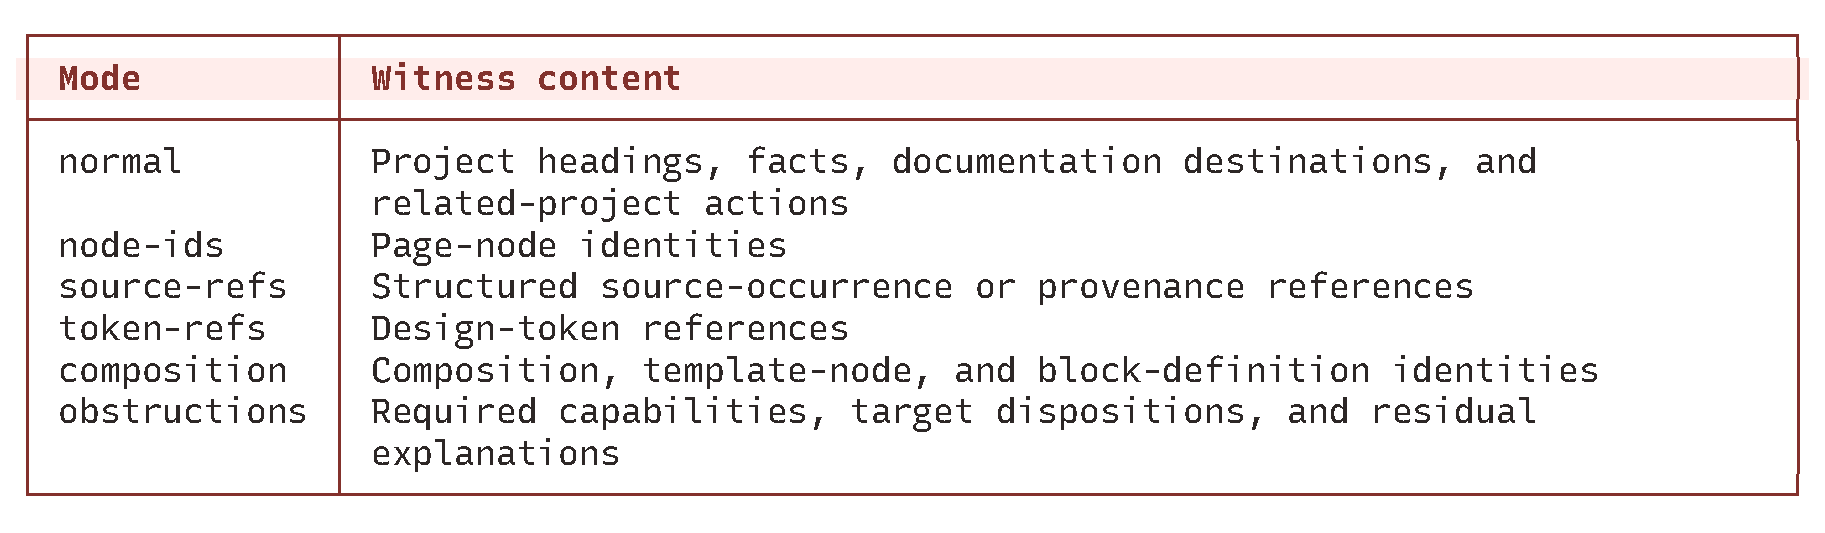
\includegraphics[width=\linewidth]{figures/tables/table-013-g1-1.pdf}
\par\smallskip{\scriptsize\color{BookMuted}Rows 1–6. Actual Bijou table component.}
\end{center}


Modes change the terminal witness. They do not change the input identities or claim browser semantics. Unsupported modes and unowned option fields fail with \texttt{B\allowbreak{}I\allowbreak{}J\allowbreak{}O\allowbreak{}U\allowbreak{}\_\allowbreak{}P\allowbreak{}A\allowbreak{}G\allowbreak{}E\allowbreak{}\_\allowbreak{}I\allowbreak{}N\allowbreak{}P\allowbreak{}U\allowbreak{}T\allowbreak{}\_\allowbreak{}R\allowbreak{}E\allowbreak{}F\allowbreak{}E\allowbreak{}R\allowbreak{}E\allowbreak{}N\allowbreak{}C\allowbreak{}E\allowbreak{}\_\allowbreak{}I\allowbreak{}N\allowbreak{}V\allowbreak{}A\allowbreak{}L\allowbreak{}I\allowbreak{}D}. Multi-value diagnostic facts use one bounded terminal row per value so the witness preserves every fact.

\section{Outputs}\label{record-025-outputs}

\texttt{P\allowbreak{}r\allowbreak{}o\allowbreak{}f\allowbreak{}u\allowbreak{}n\allowbreak{}c\allowbreak{}t\allowbreak{}o\allowbreak{}r\allowbreak{}P\allowbreak{}a\allowbreak{}g\allowbreak{}e\allowbreak{}T\allowbreak{}a\allowbreak{}r\allowbreak{}g\allowbreak{}e\allowbreak{}t\allowbreak{}P\allowbreak{}r\allowbreak{}o\allowbreak{}o\allowbreak{}f} contains:

\begin{center}
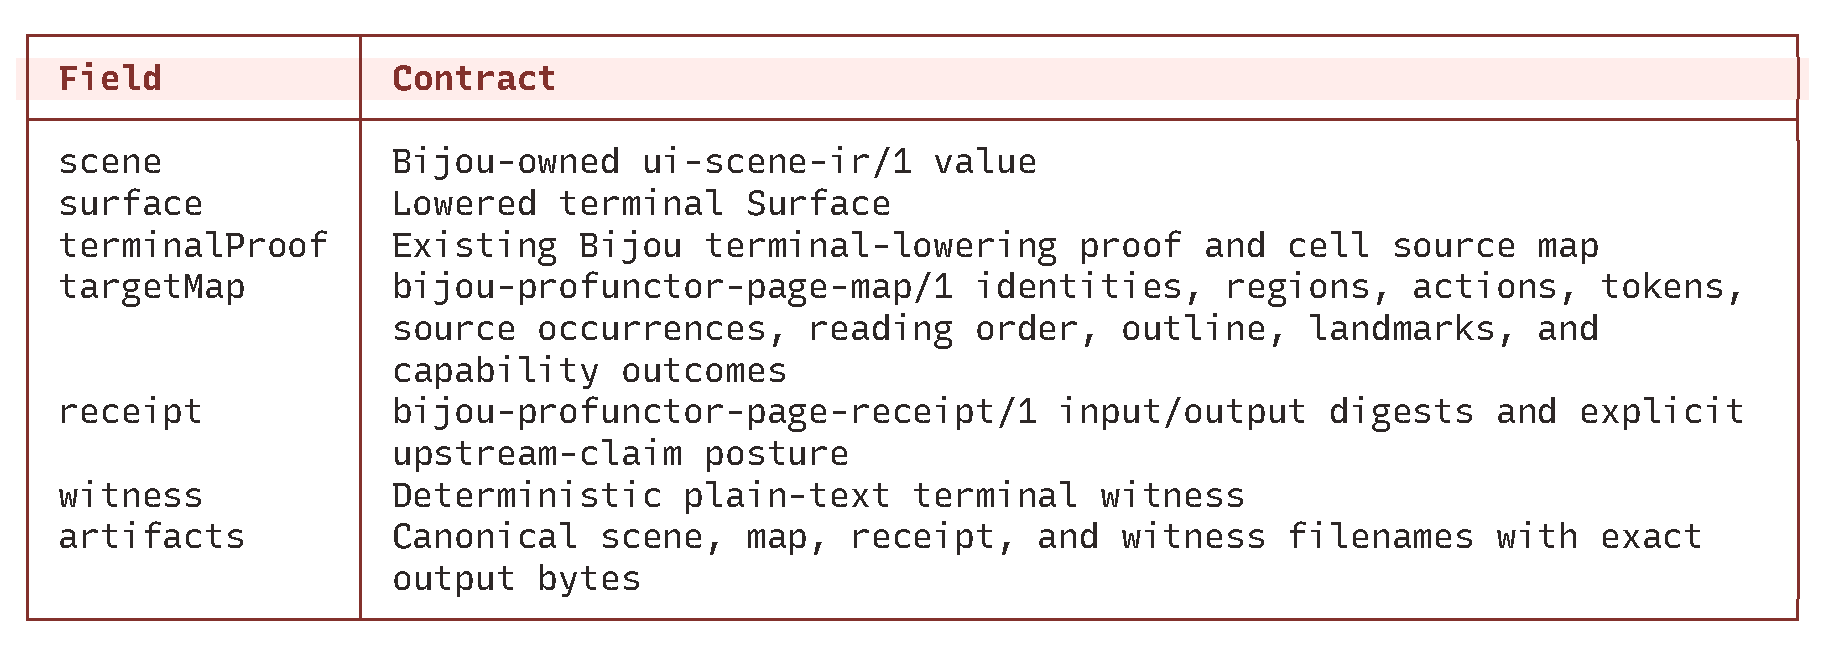
\includegraphics[width=\linewidth]{figures/tables/table-014-g1-1.pdf}
\par\smallskip{\scriptsize\color{BookMuted}Rows 1–7. Actual Bijou table component.}
\end{center}


The target preserves page, composition, override, template, content, source-occurrence, token, action, and target-render identities. Every visible page node receives one render identity. A hidden unsupported node receives one explicit residual.

Native links become Bijou action facts. Heading and landmark semantics become structural facts. Semantic HTML remains an explicit residual; the target does not inherit the build manifest's browser claims.

\section{Diagnostics}\label{record-025-diagnostics}

Failures throw \texttt{P\allowbreak{}r\allowbreak{}o\allowbreak{}f\allowbreak{}u\allowbreak{}n\allowbreak{}c\allowbreak{}t\allowbreak{}o\allowbreak{}r\allowbreak{}P\allowbreak{}a\allowbreak{}g\allowbreak{}e\allowbreak{}T\allowbreak{}a\allowbreak{}r\allowbreak{}g\allowbreak{}e\allowbreak{}t\allowbreak{}E\allowbreak{}r\allowbreak{}r\allowbreak{}o\allowbreak{}r}. Inspect \texttt{c\allowbreak{}o\allowbreak{}d\allowbreak{}e}, \texttt{p\allowbreak{}a\allowbreak{}t\allowbreak{}h}, and \texttt{d\allowbreak{}e\allowbreak{}t\allowbreak{}a\allowbreak{}i\allowbreak{}l} instead of parsing the message.

\begin{center}
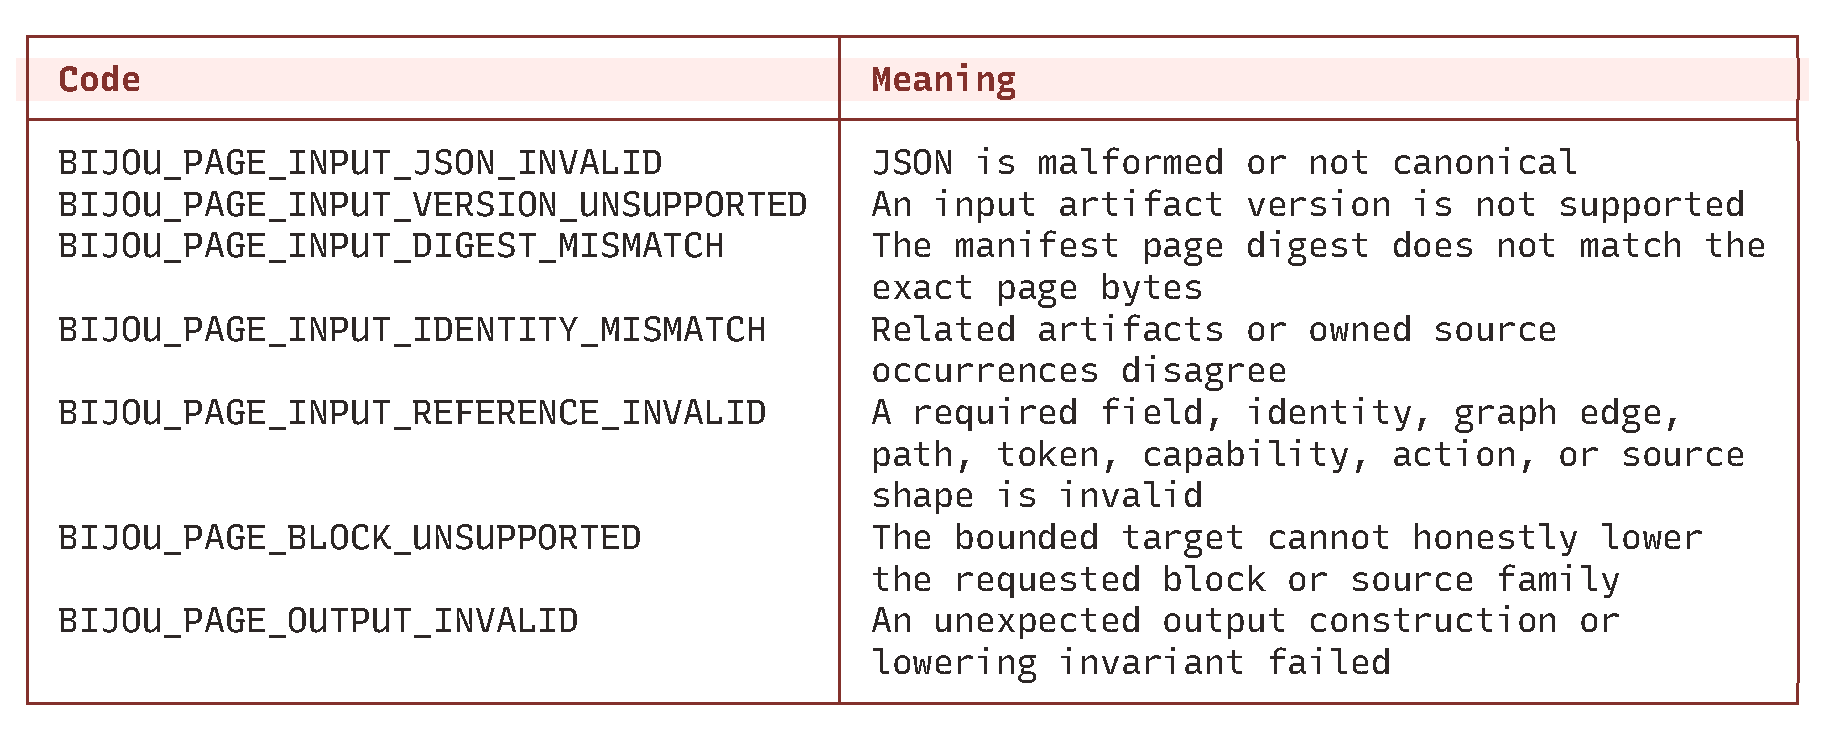
\includegraphics[width=\linewidth]{figures/tables/table-015-g1-1.pdf}
\par\smallskip{\scriptsize\color{BookMuted}Rows 1–7. Actual Bijou table component.}
\end{center}


\section{Canonical Fixture And Verification}\label{record-025-canonical-fixture-and-verification}

The checked Keep fixture pins the website-owned input bytes and the Bijou-owned outputs:

\begin{itemize}
\tightlist
\item
  \href{https://github.com/flyingrobots/bijou/blob/cbd70612140e7a450d764b3c7be1c6af878b99bc/fixtures/profunctor-page/project-keep/README.md}{Keep Profunctor Page conformance fixture}
\item
  \href{https://github.com/flyingrobots/bijou/blob/cbd70612140e7a450d764b3c7be1c6af878b99bc/docs/design/DX-050-profunctor-page-inspection.md}{DX-050 design record}
\end{itemize}

Regenerate the output artifacts:

\begin{CodeBlock}
npm run generate:profunctor-page-target
\end{CodeBlock}

Verify that the checked artifacts match the current lowerer:

\begin{CodeBlock}
npm run check:profunctor-page-target
\end{CodeBlock}

Run the focused contract evidence:

\begin{CodeBlock}
npx vitest run \
  tests/cycles/DX-050/profunctor-page-target.part01.test.ts \
  tests/cycles/DX-050/profunctor-page-target.part02.test.ts \
  tests/cycles/DX-050/profunctor-page-target.part03.test.ts \
  tests/cycles/DX-050/profunctor-page-target.part04.test.ts \
  tests/cycles/DX-050/profunctor-page-target.part05.test.ts
\end{CodeBlock}

%
\chapter{Theme Authoring Guide}\label{record-026}

\noindent{\footnotesize\color{BookMuted}\path{docs/design-system/theme-authoring.md}\par}\smallskip

This guide explains how to write your own Bijou theme, how to choose the right token family, and how to load a custom theme into a real app.

Use this together with:

\begin{itemize}
\tightlist
\item
  \href{https://github.com/flyingrobots/bijou/blob/cbd70612140e7a450d764b3c7be1c6af878b99bc/docs/design-system/theme-tokens.md}{Theme Token Vocabulary} for what each token family means
\item
  \href{https://github.com/flyingrobots/bijou/blob/cbd70612140e7a450d764b3c7be1c6af878b99bc/packages/bijou/src/core/theme/tokens.ts}{packages/bijou/src/core/theme/tokens.ts} for the raw type contract
\item
  \href{https://github.com/flyingrobots/bijou/blob/cbd70612140e7a450d764b3c7be1c6af878b99bc/packages/bijou/src/core/theme/presets.ts}{packages/bijou/src/core/theme/presets.ts} for concrete built-in examples
\end{itemize}

\section{What a Bijou theme contains}\label{record-026-what-a-bijou-theme-contains}

Every Bijou theme has these top-level groups:

\begin{itemize}
\tightlist
\item
  \texttt{n\allowbreak{}a\allowbreak{}m\allowbreak{}e}
\item
  \texttt{s\allowbreak{}t\allowbreak{}a\allowbreak{}t\allowbreak{}u\allowbreak{}s}
\item
  \texttt{s\allowbreak{}e\allowbreak{}m\allowbreak{}a\allowbreak{}n\allowbreak{}t\allowbreak{}i\allowbreak{}c}
\item
  \texttt{g\allowbreak{}r\allowbreak{}a\allowbreak{}d\allowbreak{}i\allowbreak{}e\allowbreak{}n\allowbreak{}t}
\item
  \texttt{b\allowbreak{}o\allowbreak{}r\allowbreak{}d\allowbreak{}e\allowbreak{}r}
\item
  \texttt{u\allowbreak{}i}
\item
  \texttt{s\allowbreak{}u\allowbreak{}r\allowbreak{}f\allowbreak{}a\allowbreak{}c\allowbreak{}e}
\end{itemize}

The built-in required keys inside those groups are:

\begin{itemize}
\tightlist
\item
  \texttt{s\allowbreak{}t\allowbreak{}a\allowbreak{}t\allowbreak{}u\allowbreak{}s}: \texttt{s\allowbreak{}u\allowbreak{}c\allowbreak{}c\allowbreak{}e\allowbreak{}s\allowbreak{}s}, \texttt{e\allowbreak{}r\allowbreak{}r\allowbreak{}o\allowbreak{}r}, \texttt{w\allowbreak{}a\allowbreak{}r\allowbreak{}n\allowbreak{}i\allowbreak{}n\allowbreak{}g}, \texttt{i\allowbreak{}n\allowbreak{}f\allowbreak{}o}, \texttt{p\allowbreak{}e\allowbreak{}n\allowbreak{}d\allowbreak{}i\allowbreak{}n\allowbreak{}g}, \texttt{a\allowbreak{}c\allowbreak{}t\allowbreak{}i\allowbreak{}v\allowbreak{}e}, \texttt{m\allowbreak{}u\allowbreak{}t\allowbreak{}e\allowbreak{}d}
\item
  \texttt{s\allowbreak{}e\allowbreak{}m\allowbreak{}a\allowbreak{}n\allowbreak{}t\allowbreak{}i\allowbreak{}c}: \texttt{s\allowbreak{}u\allowbreak{}c\allowbreak{}c\allowbreak{}e\allowbreak{}s\allowbreak{}s}, \texttt{e\allowbreak{}r\allowbreak{}r\allowbreak{}o\allowbreak{}r}, \texttt{w\allowbreak{}a\allowbreak{}r\allowbreak{}n\allowbreak{}i\allowbreak{}n\allowbreak{}g}, \texttt{i\allowbreak{}n\allowbreak{}f\allowbreak{}o}, \texttt{a\allowbreak{}c\allowbreak{}c\allowbreak{}e\allowbreak{}n\allowbreak{}t}, \texttt{m\allowbreak{}u\allowbreak{}t\allowbreak{}e\allowbreak{}d}, \texttt{p\allowbreak{}r\allowbreak{}i\allowbreak{}m\allowbreak{}a\allowbreak{}r\allowbreak{}y}
\item
  \texttt{b\allowbreak{}o\allowbreak{}r\allowbreak{}d\allowbreak{}e\allowbreak{}r}: \texttt{p\allowbreak{}r\allowbreak{}i\allowbreak{}m\allowbreak{}a\allowbreak{}r\allowbreak{}y}, \texttt{s\allowbreak{}e\allowbreak{}c\allowbreak{}o\allowbreak{}n\allowbreak{}d\allowbreak{}a\allowbreak{}r\allowbreak{}y}, \texttt{s\allowbreak{}u\allowbreak{}c\allowbreak{}c\allowbreak{}e\allowbreak{}s\allowbreak{}s}, \texttt{w\allowbreak{}a\allowbreak{}r\allowbreak{}n\allowbreak{}i\allowbreak{}n\allowbreak{}g}, \texttt{e\allowbreak{}r\allowbreak{}r\allowbreak{}o\allowbreak{}r}, \texttt{m\allowbreak{}u\allowbreak{}t\allowbreak{}e\allowbreak{}d}
\item
  \texttt{u\allowbreak{}i}: \texttt{c\allowbreak{}u\allowbreak{}r\allowbreak{}s\allowbreak{}o\allowbreak{}r}, \texttt{f\allowbreak{}o\allowbreak{}c\allowbreak{}u\allowbreak{}s\allowbreak{}G\allowbreak{}u\allowbreak{}t\allowbreak{}t\allowbreak{}e\allowbreak{}r}, \texttt{s\allowbreak{}c\allowbreak{}r\allowbreak{}o\allowbreak{}l\allowbreak{}l\allowbreak{}T\allowbreak{}h\allowbreak{}u\allowbreak{}m\allowbreak{}b}, \texttt{s\allowbreak{}c\allowbreak{}r\allowbreak{}o\allowbreak{}l\allowbreak{}l\allowbreak{}T\allowbreak{}r\allowbreak{}a\allowbreak{}c\allowbreak{}k}, \texttt{s\allowbreak{}e\allowbreak{}c\allowbreak{}t\allowbreak{}i\allowbreak{}o\allowbreak{}n\allowbreak{}H\allowbreak{}e\allowbreak{}a\allowbreak{}d\allowbreak{}e\allowbreak{}r}, \texttt{l\allowbreak{}o\allowbreak{}g\allowbreak{}o}, \texttt{t\allowbreak{}a\allowbreak{}b\allowbreak{}l\allowbreak{}e\allowbreak{}H\allowbreak{}e\allowbreak{}a\allowbreak{}d\allowbreak{}e\allowbreak{}r}, \texttt{t\allowbreak{}r\allowbreak{}a\allowbreak{}c\allowbreak{}k\allowbreak{}E\allowbreak{}m\allowbreak{}p\allowbreak{}t\allowbreak{}y}
\item
  \texttt{s\allowbreak{}u\allowbreak{}r\allowbreak{}f\allowbreak{}a\allowbreak{}c\allowbreak{}e}: \texttt{p\allowbreak{}r\allowbreak{}i\allowbreak{}m\allowbreak{}a\allowbreak{}r\allowbreak{}y}, \texttt{s\allowbreak{}e\allowbreak{}c\allowbreak{}o\allowbreak{}n\allowbreak{}d\allowbreak{}a\allowbreak{}r\allowbreak{}y}, \texttt{e\allowbreak{}l\allowbreak{}e\allowbreak{}v\allowbreak{}a\allowbreak{}t\allowbreak{}e\allowbreak{}d}, \texttt{o\allowbreak{}v\allowbreak{}e\allowbreak{}r\allowbreak{}l\allowbreak{}a\allowbreak{}y}, \texttt{m\allowbreak{}u\allowbreak{}t\allowbreak{}e\allowbreak{}d}
\item
  \texttt{g\allowbreak{}r\allowbreak{}a\allowbreak{}d\allowbreak{}i\allowbreak{}e\allowbreak{}n\allowbreak{}t}: \texttt{b\allowbreak{}r\allowbreak{}a\allowbreak{}n\allowbreak{}d}, \texttt{p\allowbreak{}r\allowbreak{}o\allowbreak{}g\allowbreak{}r\allowbreak{}e\allowbreak{}s\allowbreak{}s}
\end{itemize}

If a built-in key is missing in a DTCG JSON theme, Bijou will still load the document, but that missing token resolves to a black/default placeholder. In practice, that means an incomplete theme is considered malformed even if it parses successfully.

\section{Choose tokens by job, not by color}\label{record-026-choose-tokens-by-job-not-by-color}

Before picking colors, decide what each token is responsible for:

\begin{itemize}
\tightlist
\item
  \texttt{s\allowbreak{}e\allowbreak{}m\allowbreak{}a\allowbreak{}n\allowbreak{}t\allowbreak{}i\allowbreak{}c\allowbreak{}.\allowbreak{}*} is for foreground meaning and emphasis
\item
  \texttt{s\allowbreak{}u\allowbreak{}r\allowbreak{}f\allowbreak{}a\allowbreak{}c\allowbreak{}e\allowbreak{}.\allowbreak{}*} is for fills, containment, elevation, and interruption level
\item
  \texttt{b\allowbreak{}o\allowbreak{}r\allowbreak{}d\allowbreak{}e\allowbreak{}r\allowbreak{}.\allowbreak{}*} is for structure and boundary emphasis
\item
  \texttt{u\allowbreak{}i\allowbreak{}.\allowbreak{}*} is for reusable shell/runtime chrome
\item
  \texttt{s\allowbreak{}t\allowbreak{}a\allowbreak{}t\allowbreak{}u\allowbreak{}s\allowbreak{}.\allowbreak{}*} is for actual state labels and indicators
\item
  \texttt{g\allowbreak{}r\allowbreak{}a\allowbreak{}d\allowbreak{}i\allowbreak{}e\allowbreak{}n\allowbreak{}t\allowbreak{}.\allowbreak{}*} is for rare decorative or continuous-range emphasis
\end{itemize}

If you need the rulebook for those meanings, read \href{https://github.com/flyingrobots/bijou/blob/cbd70612140e7a450d764b3c7be1c6af878b99bc/docs/design-system/theme-tokens.md}{Theme Token Vocabulary} first. This guide is about authoring and loading; that guide is about semantics.

\section{Token value shape}\label{record-026-token-value-shape}

A color token can be either:

\begin{itemize}
\tightlist
\item
  a simple foreground hex string, like \texttt{"\allowbreak{}\#\allowbreak{}8\allowbreak{}8\allowbreak{}c\allowbreak{}0\allowbreak{}d\allowbreak{}0\allowbreak{}"}
\item
  or an object with:

  \begin{itemize}
  \tightlist
  \item
    \texttt{h\allowbreak{}e\allowbreak{}x}
  \item
    optional \texttt{b\allowbreak{}g}
  \item
    optional \texttt{m\allowbreak{}o\allowbreak{}d\allowbreak{}i\allowbreak{}f\allowbreak{}i\allowbreak{}e\allowbreak{}r\allowbreak{}s}
  \end{itemize}
\end{itemize}

Supported modifiers are:

\begin{itemize}
\tightlist
\item
  \texttt{b\allowbreak{}o\allowbreak{}l\allowbreak{}d}
\item
  \texttt{d\allowbreak{}i\allowbreak{}m}
\item
  \texttt{s\allowbreak{}t\allowbreak{}r\allowbreak{}i\allowbreak{}k\allowbreak{}e\allowbreak{}t\allowbreak{}h\allowbreak{}r\allowbreak{}o\allowbreak{}u\allowbreak{}g\allowbreak{}h}
\item
  \texttt{i\allowbreak{}n\allowbreak{}v\allowbreak{}e\allowbreak{}r\allowbreak{}s\allowbreak{}e}
\item
  \texttt{u\allowbreak{}n\allowbreak{}d\allowbreak{}e\allowbreak{}r\allowbreak{}l\allowbreak{}i\allowbreak{}n\allowbreak{}e}
\item
  \texttt{c\allowbreak{}u\allowbreak{}r\allowbreak{}l\allowbreak{}y\allowbreak{}-\allowbreak{}u\allowbreak{}n\allowbreak{}d\allowbreak{}e\allowbreak{}r\allowbreak{}l\allowbreak{}i\allowbreak{}n\allowbreak{}e}
\item
  \texttt{d\allowbreak{}o\allowbreak{}t\allowbreak{}t\allowbreak{}e\allowbreak{}d\allowbreak{}-\allowbreak{}u\allowbreak{}n\allowbreak{}d\allowbreak{}e\allowbreak{}r\allowbreak{}l\allowbreak{}i\allowbreak{}n\allowbreak{}e}
\item
  \texttt{d\allowbreak{}a\allowbreak{}s\allowbreak{}h\allowbreak{}e\allowbreak{}d\allowbreak{}-\allowbreak{}u\allowbreak{}n\allowbreak{}d\allowbreak{}e\allowbreak{}r\allowbreak{}l\allowbreak{}i\allowbreak{}n\allowbreak{}e}
\end{itemize}

Example token values:

\begin{CodeBlock}
"primary": "#eceff4"
\end{CodeBlock}

\begin{CodeBlock}
"primary": {
  "hex": "#eceff4",
  "bg": "#2e3440",
  "modifiers": ["bold"]
}
\end{CodeBlock}

\section{The shortest working custom theme}\label{record-026-the-shortest-working-custom-theme}

If you want a file you can start from immediately, this is the smallest honest shape to copy and edit.

\begin{CodeBlock}
{
  "name": { "$value": "my-theme" },
  "status": {
    "success": { "$type": "color", "$value": "#22c55e" },
    "error": { "$type": "color", "$value": "#ef4444" },
    "warning": { "$type": "color", "$value": "#f59e0b" },
    "info": { "$type": "color", "$value": "#38bdf8" },
    "pending": { "$type": "color", "$value": { "hex": "#64748b", "modifiers": ["dim"] } },
    "active": { "$type": "color", "$value": "#38bdf8" },
    "muted": { "$type": "color", "$value": { "hex": "#64748b", "modifiers": ["dim", "strikethrough"] } }
  },
  "semantic": {
    "success": { "$type": "color", "$value": "#22c55e" },
    "error": { "$type": "color", "$value": "#ef4444" },
    "warning": { "$type": "color", "$value": "#f59e0b" },
    "info": { "$type": "color", "$value": "#38bdf8" },
    "accent": { "$type": "color", "$value": "#c084fc" },
    "muted": { "$type": "color", "$value": { "hex": "#94a3b8", "modifiers": ["dim"] } },
    "primary": { "$type": "color", "$value": { "hex": "#f8fafc", "modifiers": ["bold"] } }
  },
  "border": {
    "primary": { "$type": "color", "$value": "#38bdf8" },
    "secondary": { "$type": "color", "$value": "#c084fc" },
    "success": { "$type": "color", "$value": "#22c55e" },
    "warning": { "$type": "color", "$value": "#f59e0b" },
    "error": { "$type": "color", "$value": "#ef4444" },
    "muted": { "$type": "color", "$value": "#64748b" }
  },
  "ui": {
    "cursor": { "$type": "color", "$value": "#38bdf8" },
    "focusGutter": { "$type": "color", "$value": "#c084fc" },
    "scrollThumb": { "$type": "color", "$value": "#38bdf8" },
    "scrollTrack": { "$type": "color", "$value": "#334155" },
    "sectionHeader": { "$type": "color", "$value": { "hex": "#f8fafc", "modifiers": ["bold"] } },
    "logo": { "$type": "color", "$value": "#38bdf8" },
    "tableHeader": { "$type": "color", "$value": "#f8fafc" },
    "trackEmpty": { "$type": "color", "$value": "#1e293b" }
  },
  "surface": {
    "primary": { "$type": "color", "$value": { "hex": "#f8fafc", "bg": "#0f172a" } },
    "secondary": { "$type": "color", "$value": { "hex": "#e2e8f0", "bg": "#1e293b" } },
    "elevated": { "$type": "color", "$value": { "hex": "#f8fafc", "bg": "#334155" } },
    "overlay": { "$type": "color", "$value": { "hex": "#f8fafc", "bg": "#0f172a" } },
    "muted": { "$type": "color", "$value": { "hex": "#94a3b8", "bg": "#020617" } }
  },
  "gradient": {
    "brand": {
      "$type": "gradient",
      "$value": [
        { "pos": 0, "color": "#38bdf8" },
        { "pos": 1, "color": "#c084fc" }
      ]
    },
    "progress": {
      "$type": "gradient",
      "$value": [
        { "pos": 0, "color": "#22c55e" },
        { "pos": 1, "color": "#38bdf8" }
      ]
    }
  }
}
\end{CodeBlock}

Save that as something like \texttt{t\allowbreak{}h\allowbreak{}e\allowbreak{}m\allowbreak{}e\allowbreak{}s\allowbreak{}/\allowbreak{}m\allowbreak{}y\allowbreak{}-\allowbreak{}t\allowbreak{}h\allowbreak{}e\allowbreak{}m\allowbreak{}e\allowbreak{}.\allowbreak{}j\allowbreak{}s\allowbreak{}o\allowbreak{}n}.

\section{Loading a custom theme}\label{record-026-loading-a-custom-theme}

For Node-hosted apps, the fastest path is \texttt{B\allowbreak{}I\allowbreak{}J\allowbreak{}O\allowbreak{}U\allowbreak{}\_\allowbreak{}T\allowbreak{}H\allowbreak{}E\allowbreak{}M\allowbreak{}E}:

\begin{CodeBlock}
BIJOU_THEME=./themes/my-theme.json npm run dogfood
\end{CodeBlock}

\section{Applying a theme programmatically}\label{record-026-applying-a-theme-programmatically}

If you already have a \texttt{T\allowbreak{}h\allowbreak{}e\allowbreak{}m\allowbreak{}e} object in code, the easiest hosted path is:

\begin{CodeBlock}
import { startApp } from '@flyingrobots/bijou-node';

await startApp(app, { theme: MY_THEME });
\end{CodeBlock}

That one call creates the Node host context with your theme and uses it for the run. If the app relies on ambient \texttt{c\allowbreak{}t\allowbreak{}x} resolution, that same themed context is also registered as the default for the hosted run.

If you want explicit ownership of the context object first, use:

\begin{CodeBlock}
import { createNodeContext } from '@flyingrobots/bijou-node';

const ctx = createNodeContext({ theme: MY_THEME });
await startApp(app, { ctx });
\end{CodeBlock}

\section{Automatic light/dark theme sets}\label{record-026-automatic-lightdark-theme-sets}

If you want more than one theme, \texttt{@\allowbreak{}f\allowbreak{}l\allowbreak{}y\allowbreak{}i\allowbreak{}n\allowbreak{}g\allowbreak{}r\allowbreak{}o\allowbreak{}b\allowbreak{}o\allowbreak{}t\allowbreak{}s\allowbreak{}/\allowbreak{}b\allowbreak{}i\allowbreak{}j\allowbreak{}o\allowbreak{}u\allowbreak{}-\allowbreak{}n\allowbreak{}o\allowbreak{}d\allowbreak{}e} now supports a named theme set at the host layer:

\begin{CodeBlock}
await startApp(app, {
  themes: [
    { id: 'light', theme: LIGHT_THEME },
    { id: 'dark', theme: DARK_THEME },
  ],
  themeMode: 'auto',
});
\end{CodeBlock}

\texttt{t\allowbreak{}h\allowbreak{}e\allowbreak{}m\allowbreak{}e\allowbreak{}M\allowbreak{}o\allowbreak{}d\allowbreak{}e} accepts:

\begin{itemize}
\tightlist
\item
  \texttt{a\allowbreak{}u\allowbreak{}t\allowbreak{}o}
\item
  \texttt{l\allowbreak{}i\allowbreak{}g\allowbreak{}h\allowbreak{}t}
\item
  \texttt{d\allowbreak{}a\allowbreak{}r\allowbreak{}k}
\end{itemize}

When \texttt{t\allowbreak{}h\allowbreak{}e\allowbreak{}m\allowbreak{}e\allowbreak{}M\allowbreak{}o\allowbreak{}d\allowbreak{}e} is \texttt{a\allowbreak{}u\allowbreak{}t\allowbreak{}o}, the host uses Bijou's terminal color-scheme detection to choose the initial entry.

If your ids are not literally \texttt{l\allowbreak{}i\allowbreak{}g\allowbreak{}h\allowbreak{}t} and \texttt{d\allowbreak{}a\allowbreak{}r\allowbreak{}k}, add explicit scheme hints:

\begin{CodeBlock}
await startApp(app, {
  themes: [
    { id: 'sunrise', scheme: 'light', theme: LIGHT_THEME },
    { id: 'midnight', scheme: 'dark', theme: DARK_THEME },
  ],
  themeMode: 'auto',
});
\end{CodeBlock}

\section{User override policy}\label{record-026-user-override-policy}

There are three practical override layers:

\begin{itemize}
\tightlist
\item
  \texttt{t\allowbreak{}h\allowbreak{}e\allowbreak{}m\allowbreak{}e\allowbreak{}O\allowbreak{}v\allowbreak{}e\allowbreak{}r\allowbreak{}r\allowbreak{}i\allowbreak{}d\allowbreak{}e} for an app-owned persisted user choice
\item
  \texttt{B\allowbreak{}I\allowbreak{}J\allowbreak{}O\allowbreak{}U\allowbreak{}\_\allowbreak{}T\allowbreak{}H\allowbreak{}E\allowbreak{}M\allowbreak{}E} for host/env-driven selection
\item
  \texttt{t\allowbreak{}h\allowbreak{}e\allowbreak{}m\allowbreak{}e\allowbreak{}M\allowbreak{}o\allowbreak{}d\allowbreak{}e\allowbreak{}:\allowbreak{} \allowbreak{}'\allowbreak{}a\allowbreak{}u\allowbreak{}t\allowbreak{}o\allowbreak{}'} for light/dark automation when nothing more explicit is chosen
\end{itemize}

Example:

\begin{CodeBlock}
await startApp(app, {
  themes: [
    { id: 'light', theme: LIGHT_THEME },
    { id: 'dark', theme: DARK_THEME },
  ],
  themeMode: 'auto',
  themeOverride: savedThemeId,
});
\end{CodeBlock}

Behavior:

\begin{itemize}
\tightlist
\item
  \texttt{t\allowbreak{}h\allowbreak{}e\allowbreak{}m\allowbreak{}e\allowbreak{}O\allowbreak{}v\allowbreak{}e\allowbreak{}r\allowbreak{}r\allowbreak{}i\allowbreak{}d\allowbreak{}e} wins when it matches one of the provided entries
\item
  otherwise \texttt{B\allowbreak{}I\allowbreak{}J\allowbreak{}O\allowbreak{}U\allowbreak{}\_\allowbreak{}T\allowbreak{}H\allowbreak{}E\allowbreak{}M\allowbreak{}E} can still select a named entry by id
\item
  otherwise, if \texttt{B\allowbreak{}I\allowbreak{}J\allowbreak{}O\allowbreak{}U\allowbreak{}\_\allowbreak{}T\allowbreak{}H\allowbreak{}E\allowbreak{}M\allowbreak{}E} is set but does not resolve to a known preset, JSON theme, or named theme entry, the explicit \texttt{t\allowbreak{}h\allowbreak{}e\allowbreak{}m\allowbreak{}e} fallback wins when provided
\item
  otherwise \texttt{t\allowbreak{}h\allowbreak{}e\allowbreak{}m\allowbreak{}e\allowbreak{}M\allowbreak{}o\allowbreak{}d\allowbreak{}e} picks the initial theme
\item
  otherwise the first entry becomes the fallback
\end{itemize}

That same pattern works for any hosted app that goes through \texttt{@\allowbreak{}f\allowbreak{}l\allowbreak{}y\allowbreak{}i\allowbreak{}n\allowbreak{}g\allowbreak{}r\allowbreak{}o\allowbreak{}b\allowbreak{}o\allowbreak{}t\allowbreak{}s\allowbreak{}/\allowbreak{}b\allowbreak{}i\allowbreak{}j\allowbreak{}o\allowbreak{}u\allowbreak{}-\allowbreak{}n\allowbreak{}o\allowbreak{}d\allowbreak{}e} theme resolution.

If \texttt{B\allowbreak{}I\allowbreak{}J\allowbreak{}O\allowbreak{}U\allowbreak{}\_\allowbreak{}T\allowbreak{}H\allowbreak{}E\allowbreak{}M\allowbreak{}E} points at a \texttt{.\allowbreak{}j\allowbreak{}s\allowbreak{}o\allowbreak{}n} file, Bijou treats it as a DTCG document. If it points at a known preset name, Bijou loads the preset instead.

Examples:

\begin{CodeBlock}
BIJOU_THEME=cyan-magenta npm run dogfood
BIJOU_THEME=teal-orange-pink npm run dogfood
BIJOU_THEME=./themes/my-theme.json npm run dogfood
\end{CodeBlock}

\section{Authoring in TypeScript}\label{record-026-authoring-in-typescript}

If you own the app code and want to construct a theme in code instead of a JSON file, match the \texttt{T\allowbreak{}h\allowbreak{}e\allowbreak{}m\allowbreak{}e} type directly:

\begin{CodeBlock}
import type { Theme } from '@flyingrobots/bijou';

export const MY_THEME: Theme = {
  name: 'my-theme',
  status: {
    success: { hex: '#22c55e' },
    error: { hex: '#ef4444' },
    warning: { hex: '#f59e0b' },
    info: { hex: '#38bdf8' },
    pending: { hex: '#64748b', modifiers: ['dim'] },
    active: { hex: '#38bdf8' },
    muted: { hex: '#64748b', modifiers: ['dim', 'strikethrough'] },
  },
  semantic: {
    success: { hex: '#22c55e' },
    error: { hex: '#ef4444' },
    warning: { hex: '#f59e0b' },
    info: { hex: '#38bdf8' },
    accent: { hex: '#c084fc' },
    muted: { hex: '#94a3b8', modifiers: ['dim'] },
    primary: { hex: '#f8fafc', modifiers: ['bold'] },
  },
  border: {
    primary: { hex: '#38bdf8' },
    secondary: { hex: '#c084fc' },
    success: { hex: '#22c55e' },
    warning: { hex: '#f59e0b' },
    error: { hex: '#ef4444' },
    muted: { hex: '#64748b' },
  },
  ui: {
    cursor: { hex: '#38bdf8' },
    focusGutter: { hex: '#c084fc' },
    scrollThumb: { hex: '#38bdf8' },
    scrollTrack: { hex: '#334155' },
    sectionHeader: { hex: '#f8fafc', modifiers: ['bold'] },
    logo: { hex: '#38bdf8' },
    tableHeader: { hex: '#f8fafc' },
    trackEmpty: { hex: '#1e293b' },
  },
  surface: {
    primary: { hex: '#f8fafc', bg: '#0f172a' },
    secondary: { hex: '#e2e8f0', bg: '#1e293b' },
    elevated: { hex: '#f8fafc', bg: '#334155' },
    overlay: { hex: '#f8fafc', bg: '#0f172a' },
    muted: { hex: '#94a3b8', bg: '#020617' },
  },
  gradient: {
    brand: [
      { pos: 0, color: [56, 189, 248] },
      { pos: 1, color: [192, 132, 252] },
    ],
    progress: [
      { pos: 0, color: [34, 197, 94] },
      { pos: 1, color: [56, 189, 248] },
    ],
  },
};
\end{CodeBlock}

\section{What you may extend}\label{record-026-what-you-may-extend}

The public generic \texttt{T\allowbreak{}h\allowbreak{}e\allowbreak{}m\allowbreak{}e\allowbreak{}<\allowbreak{}S\allowbreak{},\allowbreak{} \allowbreak{}U\allowbreak{},\allowbreak{} \allowbreak{}G\allowbreak{}>} contract allows app-level extension of:

\begin{itemize}
\tightlist
\item
  \texttt{s\allowbreak{}t\allowbreak{}a\allowbreak{}t\allowbreak{}u\allowbreak{}s}
\item
  \texttt{u\allowbreak{}i}
\item
  \texttt{g\allowbreak{}r\allowbreak{}a\allowbreak{}d\allowbreak{}i\allowbreak{}e\allowbreak{}n\allowbreak{}t}
\end{itemize}

That means app code can add stable extra keys when the domain really needs them.

Good examples:

\begin{itemize}
\tightlist
\item
  extra \texttt{s\allowbreak{}t\allowbreak{}a\allowbreak{}t\allowbreak{}u\allowbreak{}s} values for a real workflow state machine
\item
  extra \texttt{u\allowbreak{}i} tokens for recurring shell chrome
\item
  extra \texttt{g\allowbreak{}r\allowbreak{}a\allowbreak{}d\allowbreak{}i\allowbreak{}e\allowbreak{}n\allowbreak{}t} keys for a stable branded effect
\end{itemize}

Bad examples:

\begin{itemize}
\tightlist
\item
  adding one-off ad hoc token keys because a single component needs a special case
\item
  using \texttt{s\allowbreak{}t\allowbreak{}a\allowbreak{}t\allowbreak{}u\allowbreak{}s\allowbreak{}.\allowbreak{}*} for focus or selection
\item
  using \texttt{s\allowbreak{}u\allowbreak{}r\allowbreak{}f\allowbreak{}a\allowbreak{}c\allowbreak{}e\allowbreak{}.\allowbreak{}*} as a generic text-emphasis bucket
\end{itemize}

\section{Practical authoring rules}\label{record-026-practical-authoring-rules}

\begin{itemize}
\tightlist
\item
  Start from a built-in preset and edit semantically, not from a blank page.
\item
  Keep foreground/background contrast honest on every \texttt{s\allowbreak{}u\allowbreak{}r\allowbreak{}f\allowbreak{}a\allowbreak{}c\allowbreak{}e\allowbreak{}.\allowbreak{}*} token.
\item
  Use \texttt{d\allowbreak{}e\allowbreak{}f\allowbreak{}i\allowbreak{}n\allowbreak{}e\allowbreak{}T\allowbreak{}h\allowbreak{}e\allowbreak{}m\allowbreak{}e\allowbreak{}S\allowbreak{}a\allowbreak{}f\allowbreak{}e\allowbreak{}P\allowbreak{}a\allowbreak{}i\allowbreak{}r\allowbreak{}s\allowbreak{}(\allowbreak{})} plus \texttt{d\allowbreak{}o\allowbreak{}c\allowbreak{}t\allowbreak{}o\allowbreak{}r\allowbreak{}T\allowbreak{}h\allowbreak{}e\allowbreak{}m\allowbreak{}e\allowbreak{}(\allowbreak{})} when an app or component needs a reusable contrast contract across multiple foreground/background roles.
\item
  Test the theme in \texttt{i\allowbreak{}n\allowbreak{}t\allowbreak{}e\allowbreak{}r\allowbreak{}a\allowbreak{}c\allowbreak{}t\allowbreak{}i\allowbreak{}v\allowbreak{}e}, \texttt{s\allowbreak{}t\allowbreak{}a\allowbreak{}t\allowbreak{}i\allowbreak{}c}, \texttt{p\allowbreak{}i\allowbreak{}p\allowbreak{}e}, and \texttt{a\allowbreak{}c\allowbreak{}c\allowbreak{}e\allowbreak{}s\allowbreak{}s\allowbreak{}i\allowbreak{}b\allowbreak{}l\allowbreak{}e} modes.
\item
  Do not rely on color alone; labels and structure still need to make sense in \texttt{n\allowbreak{}o\allowbreak{}C\allowbreak{}o\allowbreak{}l\allowbreak{}o\allowbreak{}r}, \texttt{p\allowbreak{}i\allowbreak{}p\allowbreak{}e}, and \texttt{a\allowbreak{}c\allowbreak{}c\allowbreak{}e\allowbreak{}s\allowbreak{}s\allowbreak{}i\allowbreak{}b\allowbreak{}l\allowbreak{}e} lowering.
\item
  If the theme adds recurring framework chrome, prefer extending \texttt{u\allowbreak{}i} instead of hard-coding raw colors in shell code.
\end{itemize}

\section{Where to look next}\label{record-026-where-to-look-next}

\begin{itemize}
\tightlist
\item
  \href{https://github.com/flyingrobots/bijou/blob/cbd70612140e7a450d764b3c7be1c6af878b99bc/docs/design-system/theme-tokens.md}{Theme Token Vocabulary}
\item
  \href{https://github.com/flyingrobots/bijou/blob/cbd70612140e7a450d764b3c7be1c6af878b99bc/packages/bijou/GUIDE.md}{packages/bijou/GUIDE.md}
\item
  \href{https://github.com/flyingrobots/bijou/blob/cbd70612140e7a450d764b3c7be1c6af878b99bc/packages/bijou/ADVANCED_GUIDE.md}{packages/bijou/ADVANCED\_GUIDE.md}
\item
  \href{https://github.com/flyingrobots/bijou/blob/cbd70612140e7a450d764b3c7be1c6af878b99bc/packages/bijou-node/GUIDE.md}{packages/bijou-node/GUIDE.md}
\end{itemize}

%
\chapter{Theme Rule Recipes}\label{record-027}

\noindent{\footnotesize\color{BookMuted}\path{docs/design-system/theme-rule-recipes.md}\par}\smallskip

Theme rules let Bijou themes describe how semantic colors are selected instead of only storing final hex values.

The runtime contract is unchanged:

\begin{CodeBlock}
primitive colors
  -> selector rules
    -> TokenGraph
      -> ThemeAccessors
        -> terminal rendering
\end{CodeBlock}

Rules live in \texttt{@\allowbreak{}f\allowbreak{}l\allowbreak{}y\allowbreak{}i\allowbreak{}n\allowbreak{}g\allowbreak{}r\allowbreak{}o\allowbreak{}b\allowbreak{}o\allowbreak{}t\allowbreak{}s\allowbreak{}/\allowbreak{}b\allowbreak{}i\allowbreak{}j\allowbreak{}o\allowbreak{}u}. They do not depend on external design token packages and they compile to the same \texttt{T\allowbreak{}o\allowbreak{}k\allowbreak{}e\allowbreak{}n\allowbreak{}V\allowbreak{}a\allowbreak{}l\allowbreak{}u\allowbreak{}e} objects the renderer already consumes.

Bijou dogfoods this flow for the owned \texttt{b\allowbreak{}i\allowbreak{}j\allowbreak{}o\allowbreak{}u\allowbreak{}-\allowbreak{}d\allowbreak{}a\allowbreak{}r\allowbreak{}k} and \texttt{b\allowbreak{}i\allowbreak{}j\allowbreak{}o\allowbreak{}u\allowbreak{}-\allowbreak{}l\allowbreak{}i\allowbreak{}g\allowbreak{}h\allowbreak{}t} presets: their primitive ink, brand, and surface palettes compile through \texttt{T\allowbreak{}o\allowbreak{}k\allowbreak{}e\allowbreak{}n\allowbreak{}G\allowbreak{}r\allowbreak{}a\allowbreak{}p\allowbreak{}h} rules into the same public \texttt{T\allowbreak{}h\allowbreak{}e\allowbreak{}m\allowbreak{}e} objects existing consumers already use. Legacy vivid themes and third-party palette fixtures remain literal compatibility presets.

\section{When To Use Rules}\label{record-027-when-to-use-rules}

Use a rule when a token should follow a stable decision:

\begin{itemize}
\tightlist
\item
  readable foreground on a known surface
\item
  vivid accent that must not reuse success or error
\item
  muted candidate that still clears a contrast floor
\item
  closest palette color to a target
\item
  ordered ramp position such as the middle or final stop
\end{itemize}

Do not use rules to hide one-off taste decisions. If the product needs exactly one named color, write the token directly.

\section{Primitive To Semantic Flow}\label{record-027-primitive-to-semantic-flow}

Start with primitive colors, then derive product roles from them:

\begin{CodeBlock}
import {
  bestContrastWith,
  createTokenGraph,
  mostVivid,
  scope,
} from '@flyingrobots/bijou';

const graph = createTokenGraph({
  palette: {
    ink: '#0b1020',
    paper: '#f8fafc',
    blue: '#3399ff',
    green: '#22c55e',
    red: '#ef4444',
  },
  surface: {
    primary: { fg: '#f8fafc', bg: { ref: 'palette.ink' } },
  },
  semantic: {
    primary: bestContrastWith({ ref: 'surface.primary.bg' }, scope('palette')),
    accent: mostVivid(scope('palette'), {
      against: { ref: 'surface.primary.bg' },
      minContrast: 4.5,
      not: ['palette.green', 'palette.red'],
    }),
  },
});
\end{CodeBlock}

\texttt{s\allowbreak{}e\allowbreak{}m\allowbreak{}a\allowbreak{}n\allowbreak{}t\allowbreak{}i\allowbreak{}c\allowbreak{}.\allowbreak{}p\allowbreak{}r\allowbreak{}i\allowbreak{}m\allowbreak{}a\allowbreak{}r\allowbreak{}y} is now ``the highest-contrast palette color on the primary surface.'' \texttt{s\allowbreak{}e\allowbreak{}m\allowbreak{}a\allowbreak{}n\allowbreak{}t\allowbreak{}i\allowbreak{}c\allowbreak{}.\allowbreak{}a\allowbreak{}c\allowbreak{}c\allowbreak{}e\allowbreak{}n\allowbreak{}t} is ``the most vivid readable palette color that is not reserved for success or error.''

\section{Inspect The Decision}\label{record-027-inspect-the-decision}

Rules are useful only when they can explain themselves:

\begin{CodeBlock}
const fact = graph.inspect('semantic.accent');
\end{CodeBlock}

The inspection fact includes:

\begin{itemize}
\tightlist
\item
  the rule id
\item
  the selected candidate
\item
  candidate paths and resolved colors
\item
  excluded candidates
\item
  contrast failures
\item
  dependency paths
\end{itemize}

This is the data future Theme Inspector and Theme Lab surfaces should render. They should not infer token ownership from RGB equality or screenshots.

\section{Selector Vocabulary}\label{record-027-selector-vocabulary}

\texttt{b\allowbreak{}e\allowbreak{}s\allowbreak{}t\allowbreak{}C\allowbreak{}o\allowbreak{}n\allowbreak{}t\allowbreak{}r\allowbreak{}a\allowbreak{}s\allowbreak{}t\allowbreak{}W\allowbreak{}i\allowbreak{}t\allowbreak{}h\allowbreak{}(\allowbreak{}t\allowbreak{}a\allowbreak{}r\allowbreak{}g\allowbreak{}e\allowbreak{}t\allowbreak{},\allowbreak{} \allowbreak{}c\allowbreak{}a\allowbreak{}n\allowbreak{}d\allowbreak{}i\allowbreak{}d\allowbreak{}a\allowbreak{}t\allowbreak{}e\allowbreak{}s\allowbreak{})} chooses the highest-contrast candidate.

\texttt{m\allowbreak{}i\allowbreak{}n\allowbreak{}C\allowbreak{}o\allowbreak{}n\allowbreak{}t\allowbreak{}r\allowbreak{}a\allowbreak{}s\allowbreak{}t\allowbreak{}W\allowbreak{}i\allowbreak{}t\allowbreak{}h\allowbreak{}(\allowbreak{}t\allowbreak{}a\allowbreak{}r\allowbreak{}g\allowbreak{}e\allowbreak{}t\allowbreak{},\allowbreak{} \allowbreak{}c\allowbreak{}a\allowbreak{}n\allowbreak{}d\allowbreak{}i\allowbreak{}d\allowbreak{}a\allowbreak{}t\allowbreak{}e\allowbreak{}s\allowbreak{},\allowbreak{} \allowbreak{}\{\allowbreak{} \allowbreak{}r\allowbreak{}a\allowbreak{}t\allowbreak{}i\allowbreak{}o\allowbreak{} \allowbreak{}\}\allowbreak{})} chooses the first candidate that reaches the requested contrast ratio.

\texttt{m\allowbreak{}o\allowbreak{}s\allowbreak{}t\allowbreak{}V\allowbreak{}i\allowbreak{}v\allowbreak{}i\allowbreak{}d\allowbreak{}(\allowbreak{}c\allowbreak{}a\allowbreak{}n\allowbreak{}d\allowbreak{}i\allowbreak{}d\allowbreak{}a\allowbreak{}t\allowbreak{}e\allowbreak{}s\allowbreak{},\allowbreak{} \allowbreak{}o\allowbreak{}p\allowbreak{}t\allowbreak{}i\allowbreak{}o\allowbreak{}n\allowbreak{}s\allowbreak{})} chooses the highest-chroma candidate; it is readable only when \texttt{a\allowbreak{}g\allowbreak{}a\allowbreak{}i\allowbreak{}n\allowbreak{}s\allowbreak{}t} and \texttt{m\allowbreak{}i\allowbreak{}n\allowbreak{}C\allowbreak{}o\allowbreak{}n\allowbreak{}t\allowbreak{}r\allowbreak{}a\allowbreak{}s\allowbreak{}t} are provided.

\texttt{l\allowbreak{}e\allowbreak{}a\allowbreak{}s\allowbreak{}t\allowbreak{}V\allowbreak{}i\allowbreak{}v\allowbreak{}i\allowbreak{}d\allowbreak{}(\allowbreak{}c\allowbreak{}a\allowbreak{}n\allowbreak{}d\allowbreak{}i\allowbreak{}d\allowbreak{}a\allowbreak{}t\allowbreak{}e\allowbreak{}s\allowbreak{},\allowbreak{} \allowbreak{}o\allowbreak{}p\allowbreak{}t\allowbreak{}i\allowbreak{}o\allowbreak{}n\allowbreak{}s\allowbreak{})} chooses the lowest-chroma candidate; it uses the same readability rule.

\texttt{c\allowbreak{}l\allowbreak{}o\allowbreak{}s\allowbreak{}e\allowbreak{}s\allowbreak{}t\allowbreak{}C\allowbreak{}o\allowbreak{}l\allowbreak{}o\allowbreak{}r\allowbreak{}(\allowbreak{}t\allowbreak{}a\allowbreak{}r\allowbreak{}g\allowbreak{}e\allowbreak{}t\allowbreak{},\allowbreak{} \allowbreak{}c\allowbreak{}a\allowbreak{}n\allowbreak{}d\allowbreak{}i\allowbreak{}d\allowbreak{}a\allowbreak{}t\allowbreak{}e\allowbreak{}s\allowbreak{})} chooses the closest RGB candidate.

\texttt{n\allowbreak{}t\allowbreak{}h\allowbreak{}C\allowbreak{}o\allowbreak{}l\allowbreak{}o\allowbreak{}r\allowbreak{}(\allowbreak{}c\allowbreak{}a\allowbreak{}n\allowbreak{}d\allowbreak{}i\allowbreak{}d\allowbreak{}a\allowbreak{}t\allowbreak{}e\allowbreak{}s\allowbreak{},\allowbreak{} \allowbreak{}i\allowbreak{}n\allowbreak{}d\allowbreak{}e\allowbreak{}x\allowbreak{})} chooses an ordered candidate by integer or relative index.

Candidate scopes are deterministic. \texttt{s\allowbreak{}c\allowbreak{}o\allowbreak{}p\allowbreak{}e\allowbreak{}(\allowbreak{}'\allowbreak{}p\allowbreak{}a\allowbreak{}l\allowbreak{}e\allowbreak{}t\allowbreak{}t\allowbreak{}e\allowbreak{}'\allowbreak{})} reads direct children of the \texttt{p\allowbreak{}a\allowbreak{}l\allowbreak{}e\allowbreak{}t\allowbreak{}t\allowbreak{}e} scope in definition order.

\section{Lower-Mode Rule}\label{record-027-lower-mode-rule}

Rules improve color choice. They do not make color the only source of meaning.

Every UI that consumes these tokens still needs labels, symbols, structure, or state text that survives \texttt{N\allowbreak{}O\allowbreak{}\_\allowbreak{}C\allowbreak{}O\allowbreak{}L\allowbreak{}O\allowbreak{}R}, pipe output, and accessible lowering.

%
\chapter{Theme Token Vocabulary}\label{record-028}

\noindent{\footnotesize\color{BookMuted}\path{docs/design-system/theme-tokens.md}\par}\smallskip

This document locks down the canonical token vocabulary for Bijou.

The \texttt{T\allowbreak{}h\allowbreak{}e\allowbreak{}m\allowbreak{}e} type in \href{https://github.com/flyingrobots/bijou/blob/cbd70612140e7a450d764b3c7be1c6af878b99bc/packages/bijou/src/core/theme/tokens.ts}{\texttt{p\allowbreak{}a\allowbreak{}c\allowbreak{}k\allowbreak{}a\allowbreak{}g\allowbreak{}e\allowbreak{}s\allowbreak{}/\allowbreak{}b\allowbreak{}i\allowbreak{}j\allowbreak{}o\allowbreak{}u\allowbreak{}/\allowbreak{}s\allowbreak{}r\allowbreak{}c\allowbreak{}/\allowbreak{}c\allowbreak{}o\allowbreak{}r\allowbreak{}e\allowbreak{}/\allowbreak{}t\allowbreak{}h\allowbreak{}e\allowbreak{}m\allowbreak{}e\allowbreak{}/\allowbreak{}t\allowbreak{}o\allowbreak{}k\allowbreak{}e\allowbreak{}n\allowbreak{}s\allowbreak{}.\allowbreak{}t\allowbreak{}s}} is the API truth. This page is the doctrine truth: it defines what each token family is for, what first-party components should prefer, and what counts as misuse.

\section{Why this exists}\label{record-028-why-this-exists}

Bijou already ships a typed token model:

\begin{itemize}
\tightlist
\item
  \texttt{s\allowbreak{}e\allowbreak{}m\allowbreak{}a\allowbreak{}n\allowbreak{}t\allowbreak{}i\allowbreak{}c}
\item
  \texttt{s\allowbreak{}u\allowbreak{}r\allowbreak{}f\allowbreak{}a\allowbreak{}c\allowbreak{}e}
\item
  \texttt{b\allowbreak{}o\allowbreak{}r\allowbreak{}d\allowbreak{}e\allowbreak{}r}
\item
  \texttt{u\allowbreak{}i}
\item
  \texttt{s\allowbreak{}t\allowbreak{}a\allowbreak{}t\allowbreak{}u\allowbreak{}s}
\item
  \texttt{g\allowbreak{}r\allowbreak{}a\allowbreak{}d\allowbreak{}i\allowbreak{}e\allowbreak{}n\allowbreak{}t}
\end{itemize}

What was missing was the rulebook. Without one, component authors end up choosing tokens by ``what looks right in this preset'' instead of by semantic job, and the design system drifts into an untyped color bucket.

\section{Core rule}\label{record-028-core-rule}

Choose tokens by meaning, not by color.

If a component needs a green foreground because it means ``success'', use a success token. Do not reach for whichever family currently contains a green hex value in the active preset.

\section{Canonical families}\label{record-028-canonical-families}

\subsection{\texorpdfstring{\texttt{s\allowbreak{}e\allowbreak{}m\allowbreak{}a\allowbreak{}n\allowbreak{}t\allowbreak{}i\allowbreak{}c}}{}}\label{record-028-semantic}

Use \texttt{s\allowbreak{}e\allowbreak{}m\allowbreak{}a\allowbreak{}n\allowbreak{}t\allowbreak{}i\allowbreak{}c} for general foreground meaning and emphasis inside a component.

This is the default family for:

\begin{itemize}
\tightlist
\item
  primary text emphasis
\item
  supporting or muted text
\item
  active or focused emphasis inside a component
\item
  generic semantic cues that are not domain statuses
\end{itemize}

Built-in keys:

\begin{itemize}
\tightlist
\item
  \texttt{p\allowbreak{}r\allowbreak{}i\allowbreak{}m\allowbreak{}a\allowbreak{}r\allowbreak{}y}
\item
  \texttt{m\allowbreak{}u\allowbreak{}t\allowbreak{}e\allowbreak{}d}
\item
  \texttt{a\allowbreak{}c\allowbreak{}c\allowbreak{}e\allowbreak{}n\allowbreak{}t}
\item
  \texttt{s\allowbreak{}u\allowbreak{}c\allowbreak{}c\allowbreak{}e\allowbreak{}s\allowbreak{}s}
\item
  \texttt{e\allowbreak{}r\allowbreak{}r\allowbreak{}o\allowbreak{}r}
\item
  \texttt{w\allowbreak{}a\allowbreak{}r\allowbreak{}n\allowbreak{}i\allowbreak{}n\allowbreak{}g}
\item
  \texttt{i\allowbreak{}n\allowbreak{}f\allowbreak{}o}
\end{itemize}

House rules:

\begin{itemize}
\tightlist
\item
  prefer \texttt{s\allowbreak{}e\allowbreak{}m\allowbreak{}a\allowbreak{}n\allowbreak{}t\allowbreak{}i\allowbreak{}c\allowbreak{}.\allowbreak{}p\allowbreak{}r\allowbreak{}i\allowbreak{}m\allowbreak{}a\allowbreak{}r\allowbreak{}y} for deliberate foreground emphasis
\item
  prefer \texttt{s\allowbreak{}e\allowbreak{}m\allowbreak{}a\allowbreak{}n\allowbreak{}t\allowbreak{}i\allowbreak{}c\allowbreak{}.\allowbreak{}m\allowbreak{}u\allowbreak{}t\allowbreak{}e\allowbreak{}d} for metadata, hints, and supporting text
\item
  prefer \texttt{s\allowbreak{}e\allowbreak{}m\allowbreak{}a\allowbreak{}n\allowbreak{}t\allowbreak{}i\allowbreak{}c\allowbreak{}.\allowbreak{}a\allowbreak{}c\allowbreak{}c\allowbreak{}e\allowbreak{}n\allowbreak{}t} for local active/focused affordances inside a component
\item
  do not use \texttt{s\allowbreak{}e\allowbreak{}m\allowbreak{}a\allowbreak{}n\allowbreak{}t\allowbreak{}i\allowbreak{}c\allowbreak{}.\allowbreak{}*} as a generic background-fill family
\end{itemize}

\subsection{\texorpdfstring{\texttt{s\allowbreak{}u\allowbreak{}r\allowbreak{}f\allowbreak{}a\allowbreak{}c\allowbreak{}e}}{}}\label{record-028-surface}

Use \texttt{s\allowbreak{}u\allowbreak{}r\allowbreak{}f\allowbreak{}a\allowbreak{}c\allowbreak{}e} for containment, fill, elevation, and interruption level.

This is the default family for:

\begin{itemize}
\tightlist
\item
  panel and card backgrounds
\item
  sidebars and secondary rails
\item
  elevated regions
\item
  overlays, drawers, and modal fills
\item
  muted or disabled regions
\end{itemize}

Built-in keys:

\begin{itemize}
\tightlist
\item
  \texttt{p\allowbreak{}r\allowbreak{}i\allowbreak{}m\allowbreak{}a\allowbreak{}r\allowbreak{}y}
\item
  \texttt{s\allowbreak{}e\allowbreak{}c\allowbreak{}o\allowbreak{}n\allowbreak{}d\allowbreak{}a\allowbreak{}r\allowbreak{}y}
\item
  \texttt{e\allowbreak{}l\allowbreak{}e\allowbreak{}v\allowbreak{}a\allowbreak{}t\allowbreak{}e\allowbreak{}d}
\item
  \texttt{o\allowbreak{}v\allowbreak{}e\allowbreak{}r\allowbreak{}l\allowbreak{}a\allowbreak{}y}
\item
  \texttt{m\allowbreak{}u\allowbreak{}t\allowbreak{}e\allowbreak{}d}
\end{itemize}

House rules:

\begin{itemize}
\tightlist
\item
  treat \texttt{s\allowbreak{}u\allowbreak{}r\allowbreak{}f\allowbreak{}a\allowbreak{}c\allowbreak{}e\allowbreak{}.\allowbreak{}p\allowbreak{}r\allowbreak{}i\allowbreak{}m\allowbreak{}a\allowbreak{}r\allowbreak{}y} as the default content-region fill
\item
  treat \texttt{s\allowbreak{}u\allowbreak{}r\allowbreak{}f\allowbreak{}a\allowbreak{}c\allowbreak{}e\allowbreak{}.\allowbreak{}s\allowbreak{}e\allowbreak{}c\allowbreak{}o\allowbreak{}n\allowbreak{}d\allowbreak{}a\allowbreak{}r\allowbreak{}y} as the secondary-pane or sidebar fill
\item
  treat \texttt{s\allowbreak{}u\allowbreak{}r\allowbreak{}f\allowbreak{}a\allowbreak{}c\allowbreak{}e\allowbreak{}.\allowbreak{}e\allowbreak{}l\allowbreak{}e\allowbreak{}v\allowbreak{}a\allowbreak{}t\allowbreak{}e\allowbreak{}d} as the default fill for bounded contained objects
\item
  treat \texttt{s\allowbreak{}u\allowbreak{}r\allowbreak{}f\allowbreak{}a\allowbreak{}c\allowbreak{}e\allowbreak{}.\allowbreak{}o\allowbreak{}v\allowbreak{}e\allowbreak{}r\allowbreak{}l\allowbreak{}a\allowbreak{}y} as the interruption or overlay fill
\item
  treat \texttt{s\allowbreak{}u\allowbreak{}r\allowbreak{}f\allowbreak{}a\allowbreak{}c\allowbreak{}e\allowbreak{}.\allowbreak{}m\allowbreak{}u\allowbreak{}t\allowbreak{}e\allowbreak{}d} as the disabled, inset, or de-emphasized fill
\item
  do not use surface choice to smuggle status meaning
\end{itemize}

\subsection{\texorpdfstring{\texttt{b\allowbreak{}o\allowbreak{}r\allowbreak{}d\allowbreak{}e\allowbreak{}r}}{}}\label{record-028-border}

Use \texttt{b\allowbreak{}o\allowbreak{}r\allowbreak{}d\allowbreak{}e\allowbreak{}r} for structure, grouping, and boundary emphasis.

This is the default family for:

\begin{itemize}
\tightlist
\item
  box outlines
\item
  separators that need tokenized color
\item
  severity-bearing frames when the frame itself carries meaning
\end{itemize}

Built-in keys:

\begin{itemize}
\tightlist
\item
  \texttt{p\allowbreak{}r\allowbreak{}i\allowbreak{}m\allowbreak{}a\allowbreak{}r\allowbreak{}y}
\item
  \texttt{s\allowbreak{}e\allowbreak{}c\allowbreak{}o\allowbreak{}n\allowbreak{}d\allowbreak{}a\allowbreak{}r\allowbreak{}y}
\item
  \texttt{s\allowbreak{}u\allowbreak{}c\allowbreak{}c\allowbreak{}e\allowbreak{}s\allowbreak{}s}
\item
  \texttt{w\allowbreak{}a\allowbreak{}r\allowbreak{}n\allowbreak{}i\allowbreak{}n\allowbreak{}g}
\item
  \texttt{e\allowbreak{}r\allowbreak{}r\allowbreak{}o\allowbreak{}r}
\item
  \texttt{m\allowbreak{}u\allowbreak{}t\allowbreak{}e\allowbreak{}d}
\end{itemize}

House rules:

\begin{itemize}
\tightlist
\item
  prefer \texttt{b\allowbreak{}o\allowbreak{}r\allowbreak{}d\allowbreak{}e\allowbreak{}r\allowbreak{}.\allowbreak{}m\allowbreak{}u\allowbreak{}t\allowbreak{}e\allowbreak{}d} for ordinary structure
\item
  use \texttt{b\allowbreak{}o\allowbreak{}r\allowbreak{}d\allowbreak{}e\allowbreak{}r\allowbreak{}.\allowbreak{}p\allowbreak{}r\allowbreak{}i\allowbreak{}m\allowbreak{}a\allowbreak{}r\allowbreak{}y} or \texttt{b\allowbreak{}o\allowbreak{}r\allowbreak{}d\allowbreak{}e\allowbreak{}r\allowbreak{}.\allowbreak{}s\allowbreak{}e\allowbreak{}c\allowbreak{}o\allowbreak{}n\allowbreak{}d\allowbreak{}a\allowbreak{}r\allowbreak{}y} for stronger non-status grouping
\item
  use status-colored borders only when the border itself is part of the state
\item
  do not use warning/error borders as decoration
\end{itemize}

\subsection{\texorpdfstring{\texttt{u\allowbreak{}i}}{}}\label{record-028-ui}

Use \texttt{u\allowbreak{}i} for runtime chrome and reusable system affordances that do not belong to domain data.

This is the default family for:

\begin{itemize}
\tightlist
\item
  cursor or selection chrome owned by the shell/runtime
\item
  focused pane gutters owned by reusable shell frames
\item
  scrollbars and tracks
\item
  section headers
\item
  logos or branded shell marks
\item
  table headers when they are part of reusable framework chrome
\item
  empty tracks and similar UI scaffolding
\end{itemize}

Built-in keys:

\begin{itemize}
\tightlist
\item
  \texttt{c\allowbreak{}u\allowbreak{}r\allowbreak{}s\allowbreak{}o\allowbreak{}r}
\item
  \texttt{f\allowbreak{}o\allowbreak{}c\allowbreak{}u\allowbreak{}s\allowbreak{}G\allowbreak{}u\allowbreak{}t\allowbreak{}t\allowbreak{}e\allowbreak{}r}
\item
  \texttt{s\allowbreak{}c\allowbreak{}r\allowbreak{}o\allowbreak{}l\allowbreak{}l\allowbreak{}T\allowbreak{}h\allowbreak{}u\allowbreak{}m\allowbreak{}b}
\item
  \texttt{s\allowbreak{}c\allowbreak{}r\allowbreak{}o\allowbreak{}l\allowbreak{}l\allowbreak{}T\allowbreak{}r\allowbreak{}a\allowbreak{}c\allowbreak{}k}
\item
  \texttt{s\allowbreak{}e\allowbreak{}c\allowbreak{}t\allowbreak{}i\allowbreak{}o\allowbreak{}n\allowbreak{}H\allowbreak{}e\allowbreak{}a\allowbreak{}d\allowbreak{}e\allowbreak{}r}
\item
  \texttt{l\allowbreak{}o\allowbreak{}g\allowbreak{}o}
\item
  \texttt{t\allowbreak{}a\allowbreak{}b\allowbreak{}l\allowbreak{}e\allowbreak{}H\allowbreak{}e\allowbreak{}a\allowbreak{}d\allowbreak{}e\allowbreak{}r}
\item
  \texttt{t\allowbreak{}r\allowbreak{}a\allowbreak{}c\allowbreak{}k\allowbreak{}E\allowbreak{}m\allowbreak{}p\allowbreak{}t\allowbreak{}y}
\end{itemize}

House rules:

\begin{itemize}
\tightlist
\item
  reserve \texttt{u\allowbreak{}i\allowbreak{}.\allowbreak{}*} for framework/runtime chrome, not business-domain statuses
\item
  prefer a dedicated \texttt{u\allowbreak{}i} token when the same affordance recurs across shells
\item
  use \texttt{u\allowbreak{}i\allowbreak{}.\allowbreak{}f\allowbreak{}o\allowbreak{}c\allowbreak{}u\allowbreak{}s\allowbreak{}G\allowbreak{}u\allowbreak{}t\allowbreak{}t\allowbreak{}e\allowbreak{}r} for focused shell pane gutters; use \texttt{s\allowbreak{}e\allowbreak{}m\allowbreak{}a\allowbreak{}n\allowbreak{}t\allowbreak{}i\allowbreak{}c\allowbreak{}.\allowbreak{}a\allowbreak{}c\allowbreak{}c\allowbreak{}e\allowbreak{}n\allowbreak{}t} for local active emphasis inside a component
\item
  do not use \texttt{u\allowbreak{}i\allowbreak{}.\allowbreak{}*} as a back door for arbitrary one-off component colors
\end{itemize}

\subsection{\texorpdfstring{\texttt{s\allowbreak{}t\allowbreak{}a\allowbreak{}t\allowbreak{}u\allowbreak{}s}}{}}\label{record-028-status}

Use \texttt{s\allowbreak{}t\allowbreak{}a\allowbreak{}t\allowbreak{}u\allowbreak{}s} for explicit state labels and indicators attached to an object, process, or record.

This is the default family for:

\begin{itemize}
\tightlist
\item
  badges
\item
  timeline states
\item
  health/readiness indicators
\item
  process states such as pending or active
\end{itemize}

Built-in keys:

\begin{itemize}
\tightlist
\item
  \texttt{s\allowbreak{}u\allowbreak{}c\allowbreak{}c\allowbreak{}e\allowbreak{}s\allowbreak{}s}
\item
  \texttt{e\allowbreak{}r\allowbreak{}r\allowbreak{}o\allowbreak{}r}
\item
  \texttt{w\allowbreak{}a\allowbreak{}r\allowbreak{}n\allowbreak{}i\allowbreak{}n\allowbreak{}g}
\item
  \texttt{i\allowbreak{}n\allowbreak{}f\allowbreak{}o}
\item
  \texttt{p\allowbreak{}e\allowbreak{}n\allowbreak{}d\allowbreak{}i\allowbreak{}n\allowbreak{}g}
\item
  \texttt{a\allowbreak{}c\allowbreak{}t\allowbreak{}i\allowbreak{}v\allowbreak{}e}
\item
  \texttt{m\allowbreak{}u\allowbreak{}t\allowbreak{}e\allowbreak{}d}
\end{itemize}

House rules:

\begin{itemize}
\tightlist
\item
  use \texttt{s\allowbreak{}t\allowbreak{}a\allowbreak{}t\allowbreak{}u\allowbreak{}s\allowbreak{}.\allowbreak{}*} when the UI is naming or signaling a real status
\item
  prefer \texttt{s\allowbreak{}t\allowbreak{}a\allowbreak{}t\allowbreak{}u\allowbreak{}s\allowbreak{}.\allowbreak{}p\allowbreak{}e\allowbreak{}n\allowbreak{}d\allowbreak{}i\allowbreak{}n\allowbreak{}g} and \texttt{s\allowbreak{}t\allowbreak{}a\allowbreak{}t\allowbreak{}u\allowbreak{}s\allowbreak{}.\allowbreak{}a\allowbreak{}c\allowbreak{}t\allowbreak{}i\allowbreak{}v\allowbreak{}e} over reusing accent/focus tokens
\item
  do not use \texttt{s\allowbreak{}t\allowbreak{}a\allowbreak{}t\allowbreak{}u\allowbreak{}s\allowbreak{}.\allowbreak{}*} for focus, hover, or generic ``selected'' styling
\end{itemize}

\subsection{\texorpdfstring{\texttt{g\allowbreak{}r\allowbreak{}a\allowbreak{}d\allowbreak{}i\allowbreak{}e\allowbreak{}n\allowbreak{}t}}{}}\label{record-028-gradient}

Use \texttt{g\allowbreak{}r\allowbreak{}a\allowbreak{}d\allowbreak{}i\allowbreak{}e\allowbreak{}n\allowbreak{}t} for rare multi-stop emphasis that is intentionally decorative or specialized.

Built-in keys:

\begin{itemize}
\tightlist
\item
  \texttt{b\allowbreak{}r\allowbreak{}a\allowbreak{}n\allowbreak{}d}
\item
  \texttt{p\allowbreak{}r\allowbreak{}o\allowbreak{}g\allowbreak{}r\allowbreak{}e\allowbreak{}s\allowbreak{}s}
\end{itemize}

House rules:

\begin{itemize}
\tightlist
\item
  gradients are optional emphasis, not required meaning
\item
  never make critical status, navigation, or instructions depend on a gradient
\item
  prefer \texttt{g\allowbreak{}r\allowbreak{}a\allowbreak{}d\allowbreak{}i\allowbreak{}e\allowbreak{}n\allowbreak{}t\allowbreak{}.\allowbreak{}p\allowbreak{}r\allowbreak{}o\allowbreak{}g\allowbreak{}r\allowbreak{}e\allowbreak{}s\allowbreak{}s} only when the component is actually showing a progress fill or similar continuous range
\item
  keep logos and brand treatments rare
\end{itemize}

\section{Per-Token Library Reference}\label{record-028-per-token-library-reference}

Every token below is a role, not a paint name. The examples are intentionally strict so components remain readable when a theme changes.

\subsection{Semantic Tokens}\label{record-028-semantic-tokens}

\begin{center}
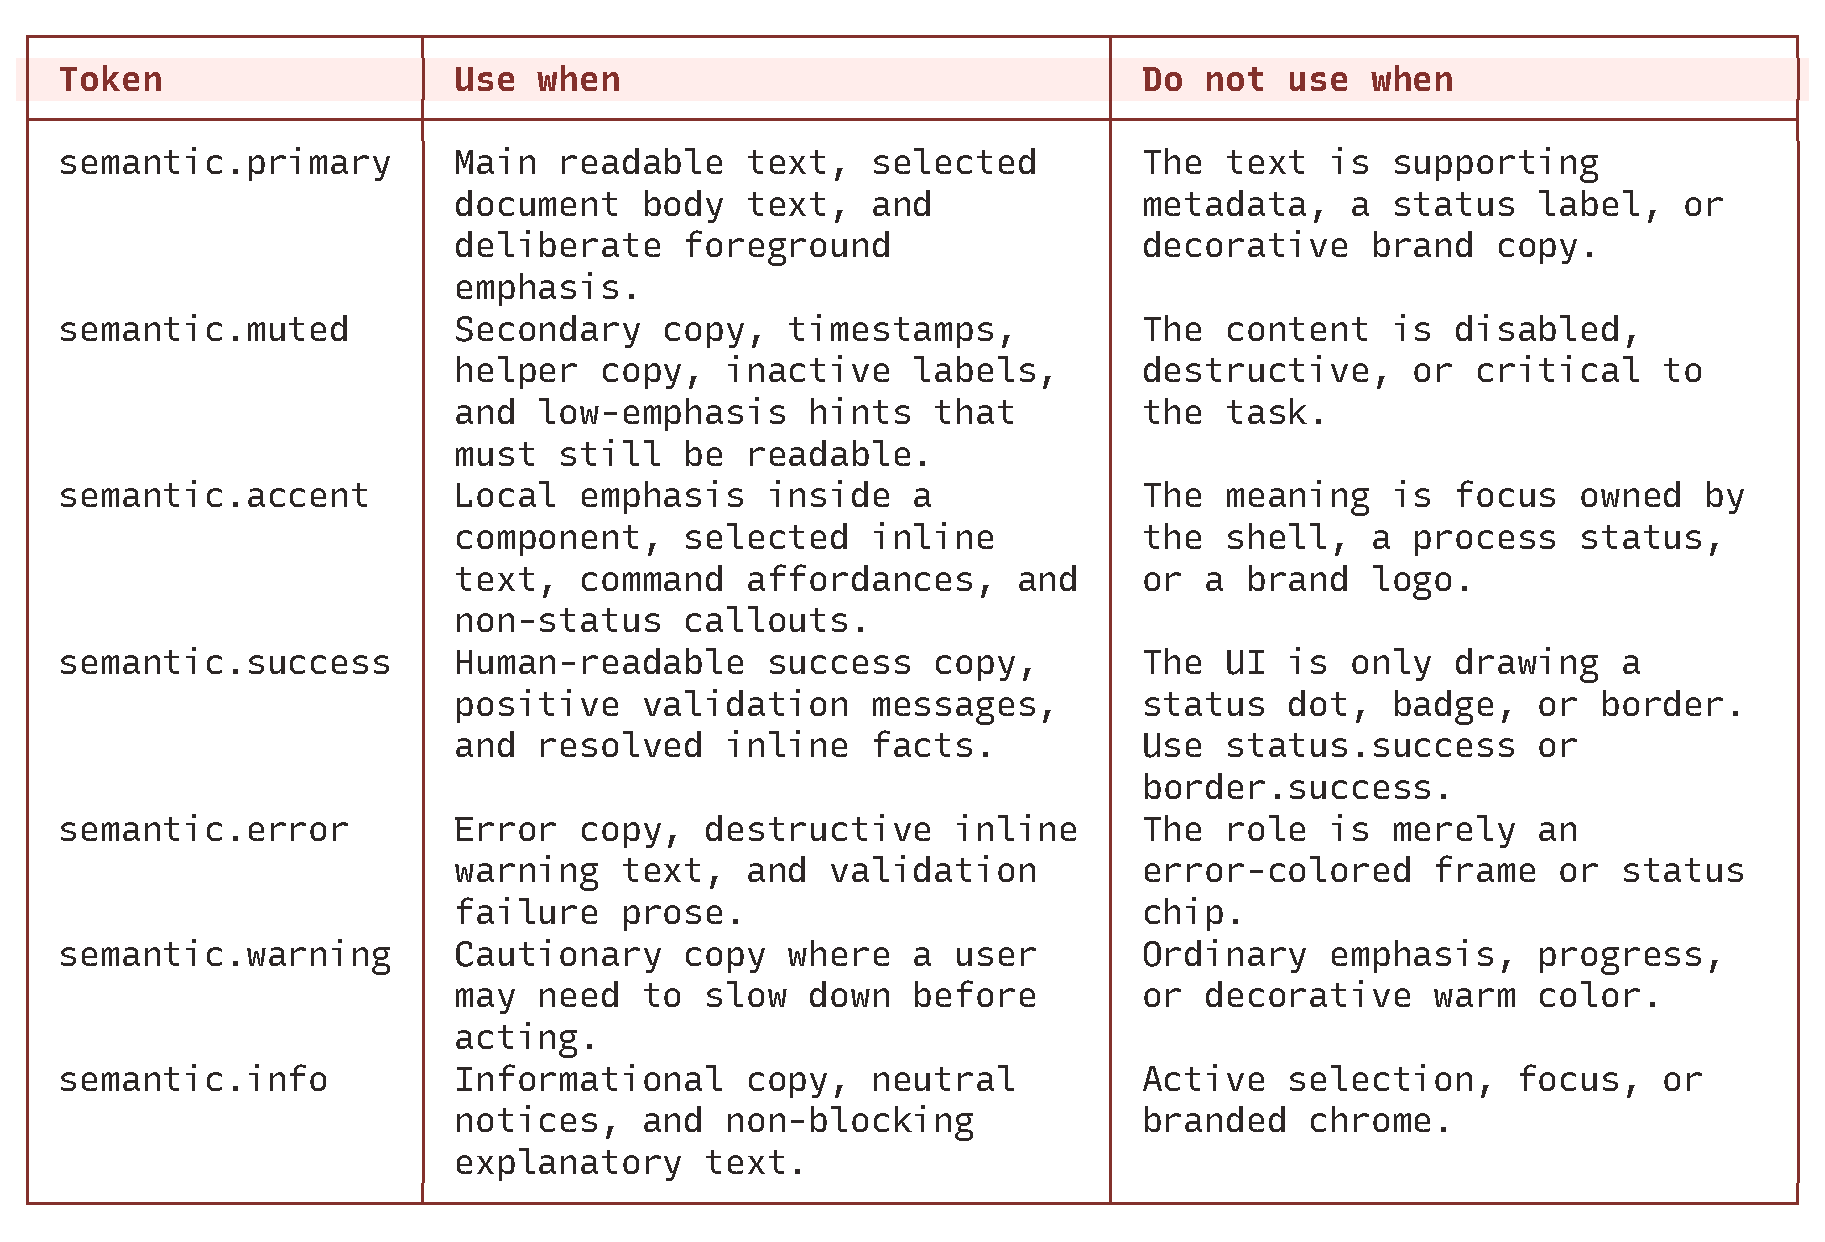
\includegraphics[width=\linewidth]{figures/tables/table-016-g1-1.pdf}
\par\smallskip{\scriptsize\color{BookMuted}Rows 1–7. Actual Bijou table component.}
\end{center}


\subsection{Surface Tokens}\label{record-028-surface-tokens}

\begin{center}
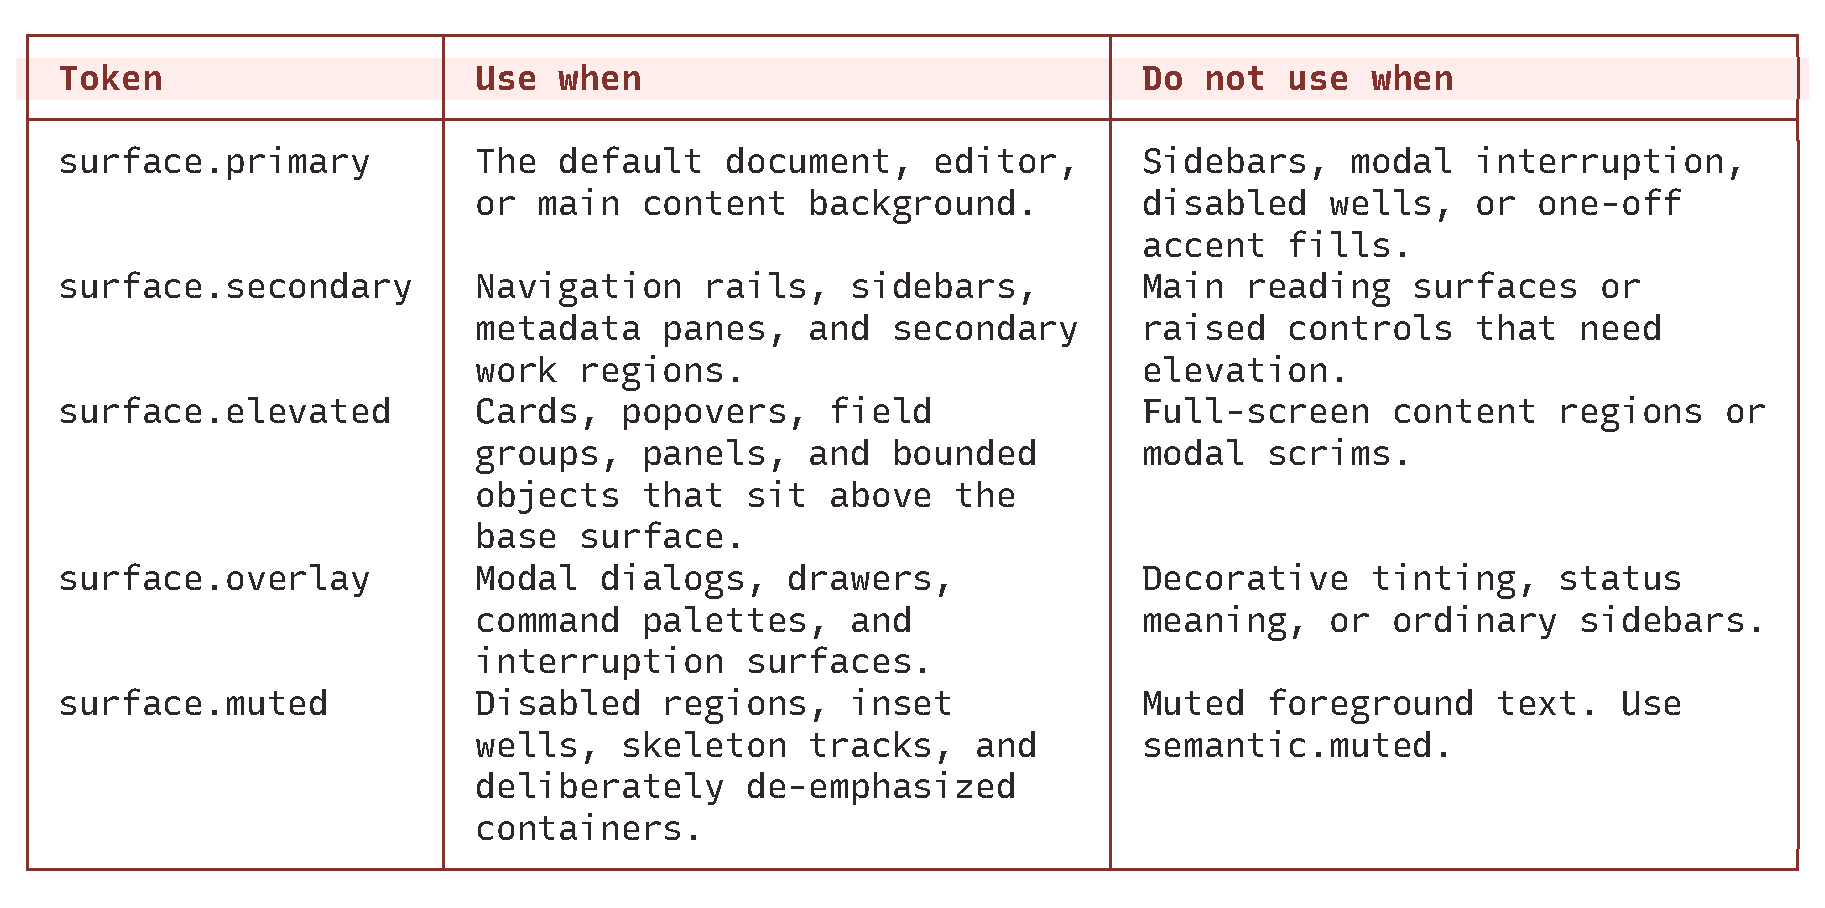
\includegraphics[width=\linewidth]{figures/tables/table-017-g1-1.pdf}
\par\smallskip{\scriptsize\color{BookMuted}Rows 1–5. Actual Bijou table component.}
\end{center}


\subsection{Border Tokens}\label{record-028-border-tokens}

\begin{center}
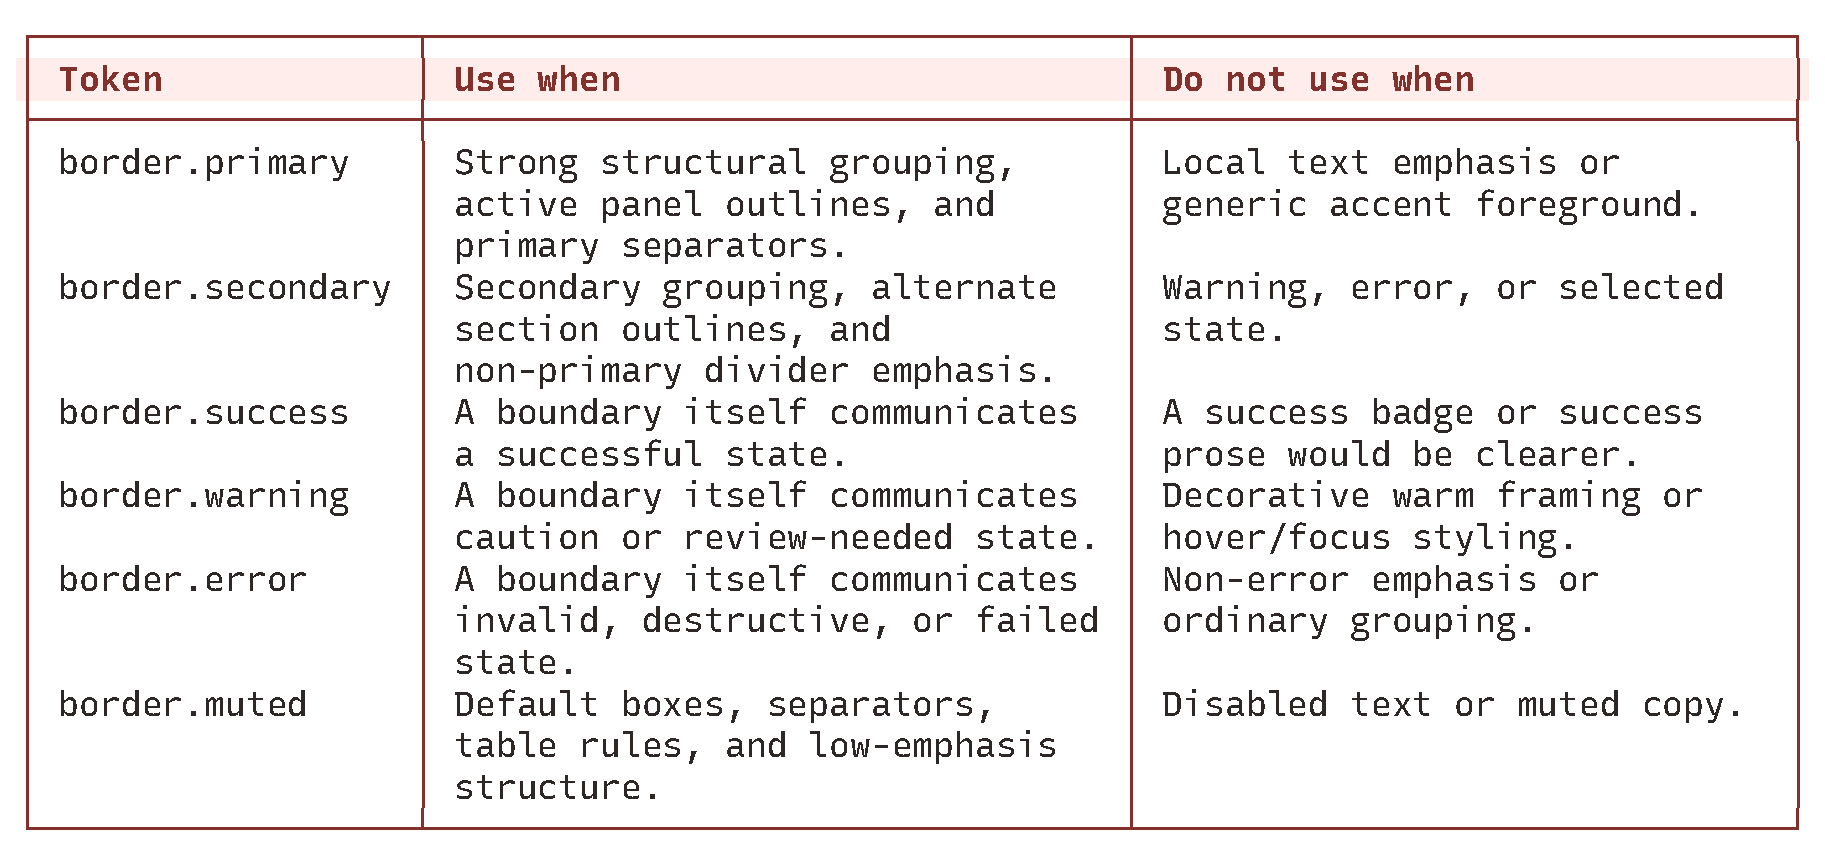
\includegraphics[width=\linewidth]{figures/tables/table-018-g1-1.pdf}
\par\smallskip{\scriptsize\color{BookMuted}Rows 1–6. Actual Bijou table component.}
\end{center}


\subsection{UI Tokens}\label{record-028-ui-tokens}

\begin{center}
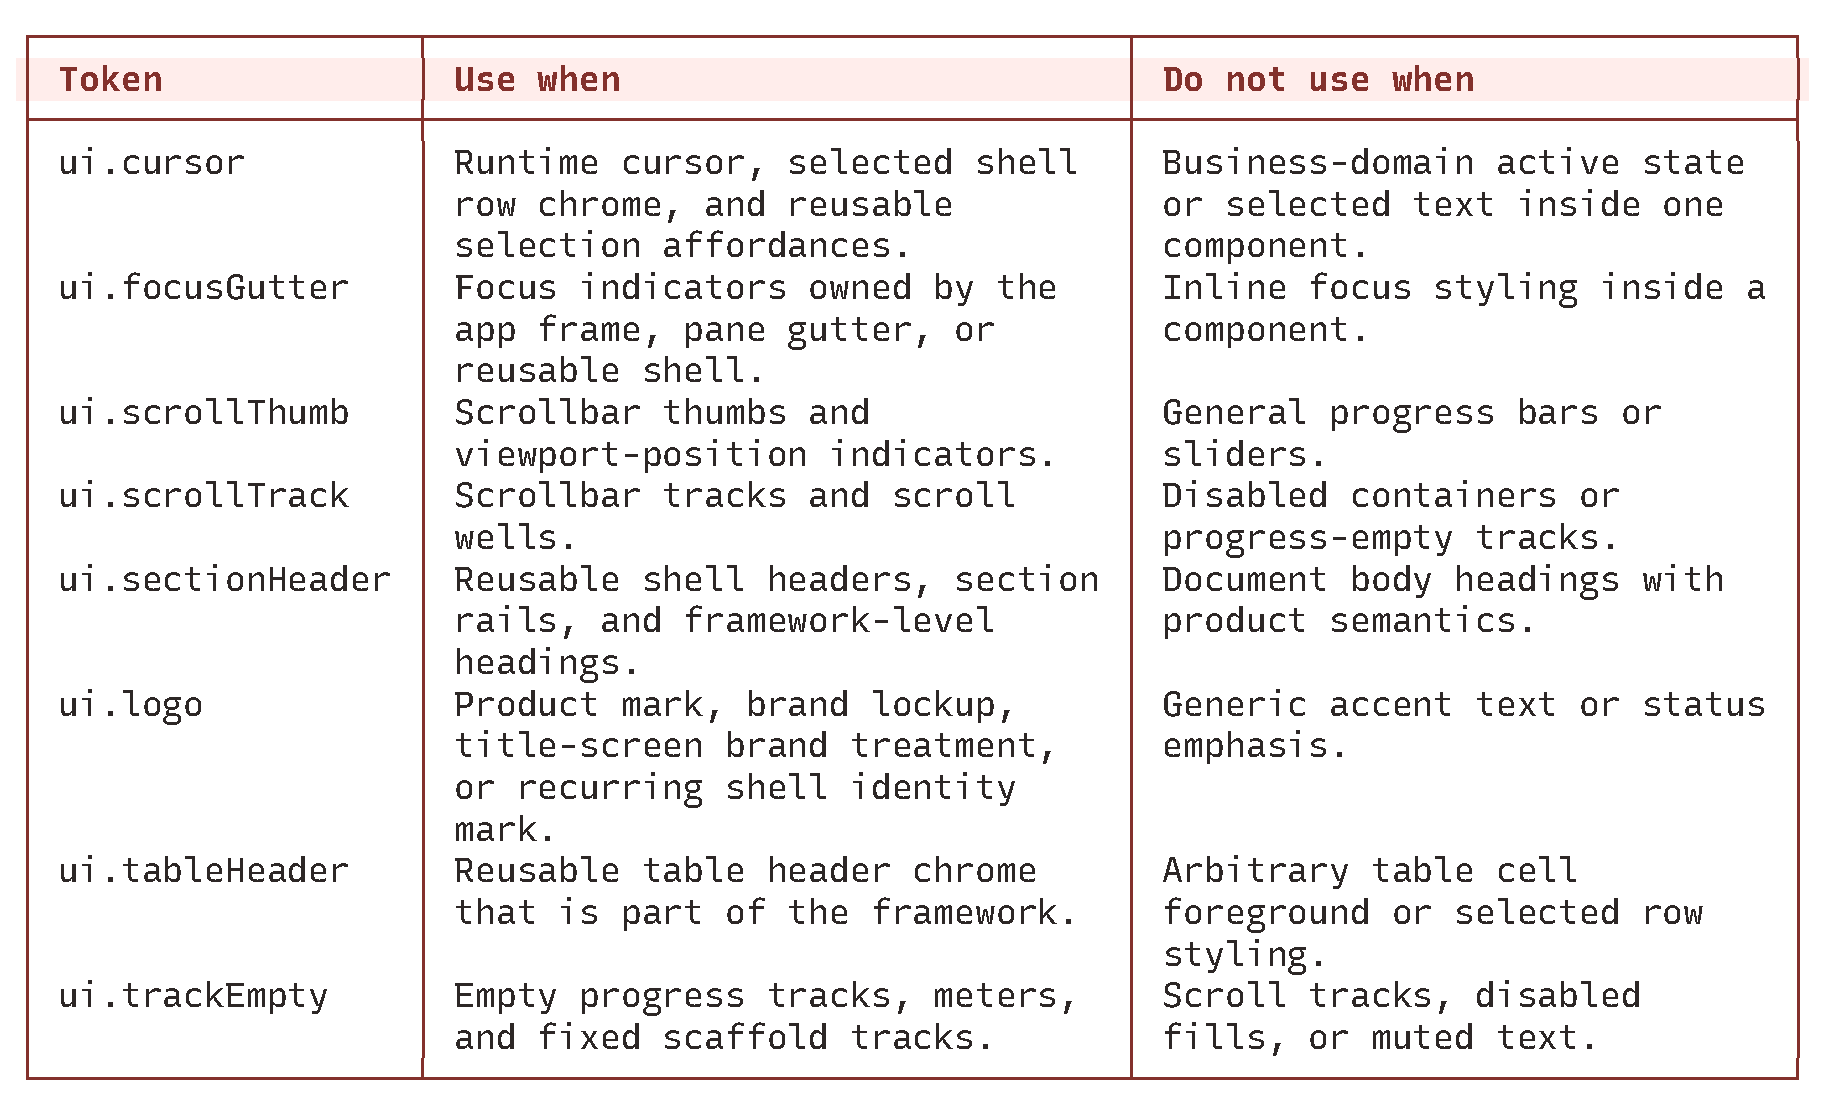
\includegraphics[width=\linewidth]{figures/tables/table-019-g1-1.pdf}
\par\smallskip{\scriptsize\color{BookMuted}Rows 1–8. Actual Bijou table component.}
\end{center}


\subsection{Status Tokens}\label{record-028-status-tokens}

\begin{center}
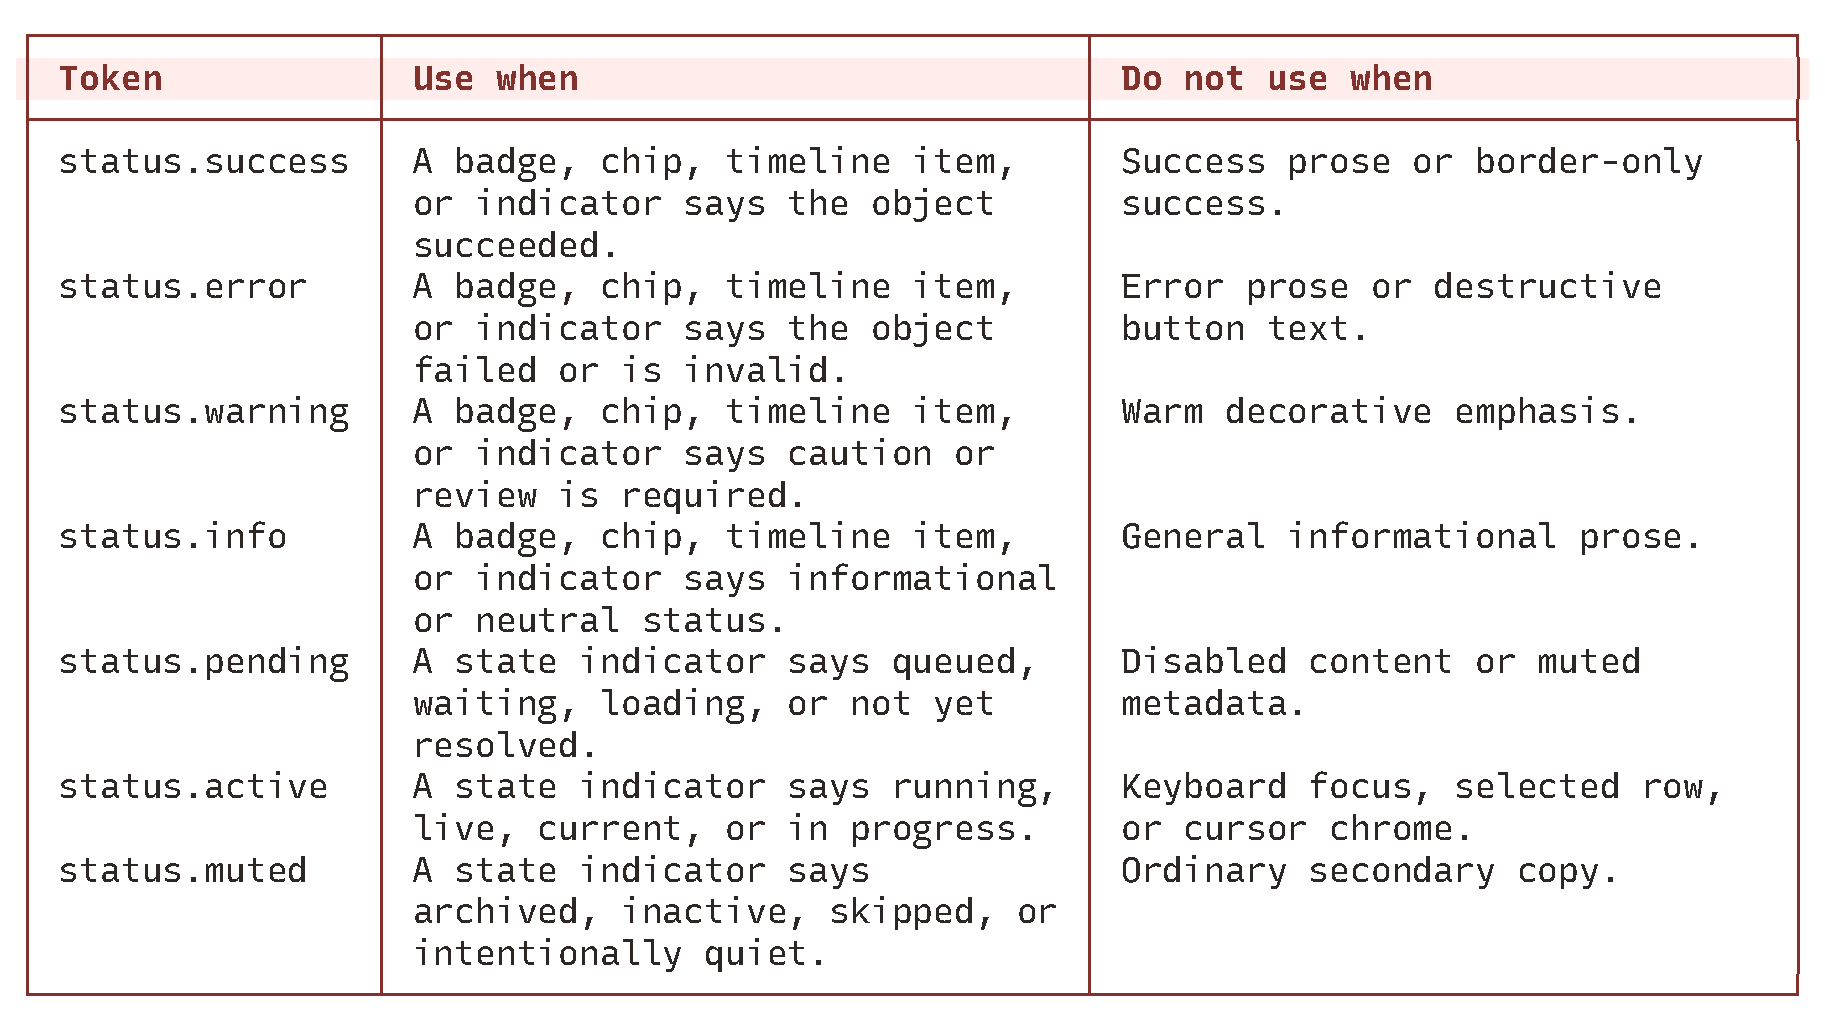
\includegraphics[width=\linewidth]{figures/tables/table-020-g1-1.pdf}
\par\smallskip{\scriptsize\color{BookMuted}Rows 1–7. Actual Bijou table component.}
\end{center}


\subsection{Gradient Tokens}\label{record-028-gradient-tokens}

\begin{center}
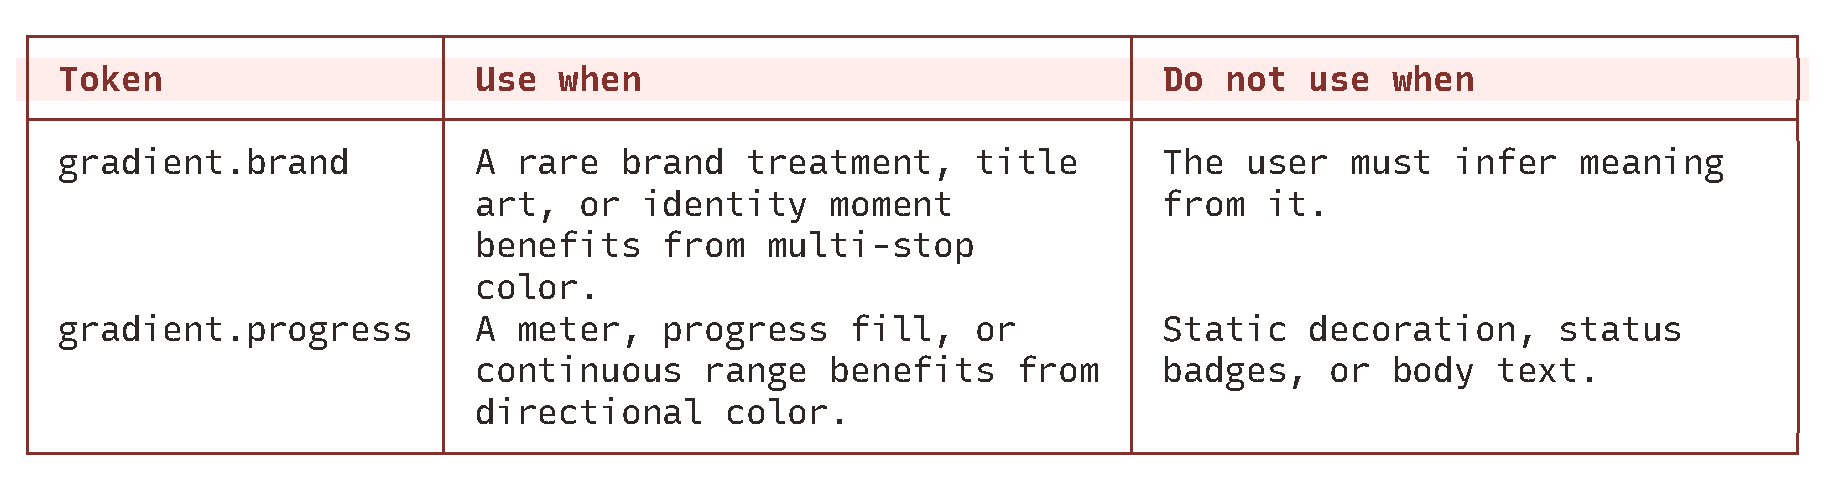
\includegraphics[width=\linewidth]{figures/tables/table-021-g1-1.pdf}
\par\smallskip{\scriptsize\color{BookMuted}Rows 1–2. Actual Bijou table component.}
\end{center}


\section{Default Dark/Light UX Audit}\label{record-028-default-darklight-ux-audit}

The legacy \texttt{C\allowbreak{}Y\allowbreak{}A\allowbreak{}N\allowbreak{}\_\allowbreak{}M\allowbreak{}A\allowbreak{}G\allowbreak{}E\allowbreak{}N\allowbreak{}T\allowbreak{}A} preset is useful as a vivid terminal-native preset, but it is not ideal as the model for dense product surfaces. It uses saturated terminal colors for many unrelated jobs: cyan appears as info, active state, cursor, scrollbar, logo, and primary border; magenta appears as accent, secondary border, and focus gutter. That makes the app energetic, but it also makes many regions compete at the same visual priority.

Bijou's first-party defaults now use a calmer shell posture:

\begin{itemize}
\tightlist
\item
  neutral surfaces carry most of the screen
\item
  one accent family carries local emphasis and shell selection
\item
  status colors remain distinct from focus and brand
\item
  muted text remains contrast-safe instead of merely dim
\item
  dark and light themes both satisfy readable foreground/background pairs
\end{itemize}

The \texttt{B\allowbreak{}I\allowbreak{}J\allowbreak{}O\allowbreak{}U\allowbreak{}\_\allowbreak{}D\allowbreak{}A\allowbreak{}R\allowbreak{}K} preset uses dark neutral surfaces, readable cool/warm accents, and separate success/warning/error/info colors. The \texttt{B\allowbreak{}I\allowbreak{}J\allowbreak{}O\allowbreak{}U\allowbreak{}\_\allowbreak{}L\allowbreak{}I\allowbreak{}G\allowbreak{}H\allowbreak{}T} preset uses light neutral surfaces with darker semantic colors instead of pastel foregrounds. DOGFOOD consumes those defaults directly as one \texttt{D\allowbreak{}O\allowbreak{}G\allowbreak{}F\allowbreak{}O\allowbreak{}O\allowbreak{}D} shell theme family with \texttt{D\allowbreak{}a\allowbreak{}r\allowbreak{}k} and \texttt{L\allowbreak{}i\allowbreak{}g\allowbreak{}h\allowbreak{}t} modes, so the docs app proves the same palette family that first-party components should treat as the baseline. Both modes target at least 4.5:1 contrast for surface text and common semantic foregrounds on every shell surface.

Compared with large design systems, Bijou is intentionally compact today. The runtime vocabulary has about thirty direct color-bearing slots plus two gradient roles. Material-style systems expose more paired foreground/background roles. Carbon and Atlassian-style systems go further with text hierarchy, interaction states, icon roles, and component-specific aliases. Bijou should grow only when a missing role causes repeated ambiguity in real components.

\section{Safe-Pair Contrast Contract}\label{record-028-safe-pair-contrast-contract}

Theme contrast is declared through safe pairs rather than buried inside one-off test loops. A safe pair names a foreground token path and a background token path that a theme promises will remain readable.

Safe-pair background paths may target token background slots:

\begin{CodeBlock}
semantic.primary on surface.primary.bg
semantic.muted on surface.secondary.bg
status.active on surface.overlay.bg
ui.cursor on surface.elevated.bg
\end{CodeBlock}

Use the \texttt{d\allowbreak{}e\allowbreak{}f\allowbreak{}i\allowbreak{}n\allowbreak{}e\allowbreak{}T\allowbreak{}h\allowbreak{}e\allowbreak{}m\allowbreak{}e\allowbreak{}S\allowbreak{}a\allowbreak{}f\allowbreak{}e\allowbreak{}P\allowbreak{}a\allowbreak{}i\allowbreak{}r\allowbreak{}s\allowbreak{}(\allowbreak{})} builder when a first-party app or component needs a reusable contrast matrix:

\begin{CodeBlock}
const pairs = defineThemeSafePairs()
  .readable('semantic.primary', 'surface.primary.bg')
  .status('status.error', 'surface.overlay.bg')
  .chrome('ui.cursor', 'surface.secondary.bg')
  .build();
\end{CodeBlock}

Then pass those pairs to \texttt{d\allowbreak{}o\allowbreak{}c\allowbreak{}t\allowbreak{}o\allowbreak{}r\allowbreak{}T\allowbreak{}h\allowbreak{}e\allowbreak{}m\allowbreak{}e\allowbreak{}(\allowbreak{})}:

\begin{CodeBlock}
const report = doctorTheme(theme, { contrastPairs: pairs });
\end{CodeBlock}

Safe-pair kinds communicate intent:

\begin{itemize}
\tightlist
\item
  \texttt{r\allowbreak{}e\allowbreak{}a\allowbreak{}d\allowbreak{}a\allowbreak{}b\allowbreak{}l\allowbreak{}e}: ordinary text or component foregrounds that must stay legible
\item
  \texttt{s\allowbreak{}t\allowbreak{}a\allowbreak{}t\allowbreak{}u\allowbreak{}s}: process, health, timeline, or object-state colors
\item
  \texttt{c\allowbreak{}h\allowbreak{}r\allowbreak{}o\allowbreak{}m\allowbreak{}e}: shell/runtime affordances such as cursor and selection chrome
\end{itemize}

Do not use safe pairs as a way to bless every possible token combination. Declare pairs only when a component or product surface expects that combination to work.

\section{Theme Debugger And Lab}\label{record-028-theme-debugger-and-lab}

DOGFOOD now has two inspectability surfaces:

\begin{itemize}
\tightlist
\item
  \texttt{F\allowbreak{}1\allowbreak{}0} opens a bounded Theme Inspector drawer in the docs shell.
\item
  The \texttt{T\allowbreak{}h\allowbreak{}e\allowbreak{}m\allowbreak{}e\allowbreak{}s} page publishes a Theme Lab with default palettes, shell-gallery facts, token swatches, and safe-pair diagnostics.
\end{itemize}

Current UX:

\begin{itemize}
\tightlist
\item
  \texttt{F\allowbreak{}1\allowbreak{}0} opens the drawer on the active DOGFOOD shell theme.
\item
  \texttt{F\allowbreak{}1\allowbreak{}0} or \texttt{E\allowbreak{}s\allowbreak{}c} closes the drawer.
\item
  The drawer shows token swatches grouped by \texttt{s\allowbreak{}e\allowbreak{}m\allowbreak{}a\allowbreak{}n\allowbreak{}t\allowbreak{}i\allowbreak{}c}, \texttt{s\allowbreak{}u\allowbreak{}r\allowbreak{}f\allowbreak{}a\allowbreak{}c\allowbreak{}e}, \texttt{b\allowbreak{}o\allowbreak{}r\allowbreak{}d\allowbreak{}e\allowbreak{}r}, \texttt{u\allowbreak{}i}, \texttt{s\allowbreak{}t\allowbreak{}a\allowbreak{}t\allowbreak{}u\allowbreak{}s}, and \texttt{g\allowbreak{}r\allowbreak{}a\allowbreak{}d\allowbreak{}i\allowbreak{}e\allowbreak{}n\allowbreak{}t}.
\item
  Each swatch renders the token path and uses the token value as the swatch fill or foreground depending on token family.
\item
  The drawer reports the safe-pair pass count for the active theme.
\item
  The Theme Lab page lists the first-party dark/light defaults, DOGFOOD shell themes, landing palette themes, and token swatches.
\end{itemize}

Still deferred:

\begin{itemize}
\tightlist
\item
  dark/light preview without committing the app theme
\item
  element-level token overlays
\item
  renderer provenance that can report whether a cell came from a token, raw color, or lowered/no-color fallback
\end{itemize}

The current implementation inspects theme tokens only. Element-level token overlays should wait until renderer provenance is available, because guessing token ownership from final RGB values would be misleading.

\section{First-Party Defaults}\label{record-028-first-party-defaults}

When first-party components need a default token and do not have stronger domain-specific semantics, prefer these defaults:

\begin{itemize}
\tightlist
\item
  default supporting text: \texttt{s\allowbreak{}e\allowbreak{}m\allowbreak{}a\allowbreak{}n\allowbreak{}t\allowbreak{}i\allowbreak{}c\allowbreak{}.\allowbreak{}m\allowbreak{}u\allowbreak{}t\allowbreak{}e\allowbreak{}d}
\item
  explicit primary emphasis: \texttt{s\allowbreak{}e\allowbreak{}m\allowbreak{}a\allowbreak{}n\allowbreak{}t\allowbreak{}i\allowbreak{}c\allowbreak{}.\allowbreak{}p\allowbreak{}r\allowbreak{}i\allowbreak{}m\allowbreak{}a\allowbreak{}r\allowbreak{}y}
\item
  local active or focused affordance inside a component: \texttt{s\allowbreak{}e\allowbreak{}m\allowbreak{}a\allowbreak{}n\allowbreak{}t\allowbreak{}i\allowbreak{}c\allowbreak{}.\allowbreak{}a\allowbreak{}c\allowbreak{}c\allowbreak{}e\allowbreak{}n\allowbreak{}t}
\item
  default structural border: \texttt{b\allowbreak{}o\allowbreak{}r\allowbreak{}d\allowbreak{}e\allowbreak{}r\allowbreak{}.\allowbreak{}m\allowbreak{}u\allowbreak{}t\allowbreak{}e\allowbreak{}d}
\item
  default contained-region fill: \texttt{s\allowbreak{}u\allowbreak{}r\allowbreak{}f\allowbreak{}a\allowbreak{}c\allowbreak{}e\allowbreak{}.\allowbreak{}e\allowbreak{}l\allowbreak{}e\allowbreak{}v\allowbreak{}a\allowbreak{}t\allowbreak{}e\allowbreak{}d}
\item
  default secondary-pane fill: \texttt{s\allowbreak{}u\allowbreak{}r\allowbreak{}f\allowbreak{}a\allowbreak{}c\allowbreak{}e\allowbreak{}.\allowbreak{}s\allowbreak{}e\allowbreak{}c\allowbreak{}o\allowbreak{}n\allowbreak{}d\allowbreak{}a\allowbreak{}r\allowbreak{}y}
\item
  default overlay fill: \texttt{s\allowbreak{}u\allowbreak{}r\allowbreak{}f\allowbreak{}a\allowbreak{}c\allowbreak{}e\allowbreak{}.\allowbreak{}o\allowbreak{}v\allowbreak{}e\allowbreak{}r\allowbreak{}l\allowbreak{}a\allowbreak{}y}
\item
  default disabled or inset fill: \texttt{s\allowbreak{}u\allowbreak{}r\allowbreak{}f\allowbreak{}a\allowbreak{}c\allowbreak{}e\allowbreak{}.\allowbreak{}m\allowbreak{}u\allowbreak{}t\allowbreak{}e\allowbreak{}d}
\item
  reusable shell cursor or selected-shell chrome: \texttt{u\allowbreak{}i\allowbreak{}.\allowbreak{}c\allowbreak{}u\allowbreak{}r\allowbreak{}s\allowbreak{}o\allowbreak{}r}
\item
  reusable focused shell gutter chrome: \texttt{u\allowbreak{}i\allowbreak{}.\allowbreak{}f\allowbreak{}o\allowbreak{}c\allowbreak{}u\allowbreak{}s\allowbreak{}G\allowbreak{}u\allowbreak{}t\allowbreak{}t\allowbreak{}e\allowbreak{}r}
\item
  reusable scrollbar chrome: \texttt{u\allowbreak{}i\allowbreak{}.\allowbreak{}s\allowbreak{}c\allowbreak{}r\allowbreak{}o\allowbreak{}l\allowbreak{}l\allowbreak{}T\allowbreak{}h\allowbreak{}u\allowbreak{}m\allowbreak{}b} and \texttt{u\allowbreak{}i\allowbreak{}.\allowbreak{}s\allowbreak{}c\allowbreak{}r\allowbreak{}o\allowbreak{}l\allowbreak{}l\allowbreak{}T\allowbreak{}r\allowbreak{}a\allowbreak{}c\allowbreak{}k}
\item
  table header chrome: \texttt{u\allowbreak{}i\allowbreak{}.\allowbreak{}t\allowbreak{}a\allowbreak{}b\allowbreak{}l\allowbreak{}e\allowbreak{}H\allowbreak{}e\allowbreak{}a\allowbreak{}d\allowbreak{}e\allowbreak{}r}
\item
  progress empty track: \texttt{u\allowbreak{}i\allowbreak{}.\allowbreak{}t\allowbreak{}r\allowbreak{}a\allowbreak{}c\allowbreak{}k\allowbreak{}E\allowbreak{}m\allowbreak{}p\allowbreak{}t\allowbreak{}y}
\end{itemize}

These defaults are conventions, not excuses to skip judgment. If a component has a stronger semantic job, use the family that matches the job.

\section{First-Party Prohibitions}\label{record-028-first-party-prohibitions}

First-party components should follow these rules:

\begin{itemize}
\tightlist
\item
  do not read raw token paths from \texttt{c\allowbreak{}t\allowbreak{}x\allowbreak{}.\allowbreak{}t\allowbreak{}h\allowbreak{}e\allowbreak{}m\allowbreak{}e\allowbreak{}.\allowbreak{}t\allowbreak{}h\allowbreak{}e\allowbreak{}m\allowbreak{}e\allowbreak{}.\allowbreak{}*} when an accessor exists
\item
  do not invent new first-party token families ad hoc
\item
  do not use \texttt{s\allowbreak{}t\allowbreak{}a\allowbreak{}t\allowbreak{}u\allowbreak{}s\allowbreak{}.\allowbreak{}*} when the real meaning is focus or selection
\item
  do not use \texttt{s\allowbreak{}u\allowbreak{}r\allowbreak{}f\allowbreak{}a\allowbreak{}c\allowbreak{}e\allowbreak{}.\allowbreak{}*} as a generic foreground-emphasis bucket
\item
  do not use gradients as a substitute for semantic color
\item
  do not rely on color alone; meaning must survive \texttt{n\allowbreak{}o\allowbreak{}C\allowbreak{}o\allowbreak{}l\allowbreak{}o\allowbreak{}r}, \texttt{p\allowbreak{}i\allowbreak{}p\allowbreak{}e}, and \texttt{a\allowbreak{}c\allowbreak{}c\allowbreak{}e\allowbreak{}s\allowbreak{}s\allowbreak{}i\allowbreak{}b\allowbreak{}l\allowbreak{}e}
\end{itemize}

If the current token families are not expressive enough, change the theme contract and docs in the same slice instead of sneaking around the vocabulary.

\section{Extension Rules}\label{record-028-extension-rules}

Third-party and app-level code may extend:

\begin{itemize}
\tightlist
\item
  \texttt{s\allowbreak{}t\allowbreak{}a\allowbreak{}t\allowbreak{}u\allowbreak{}s}
\item
  \texttt{u\allowbreak{}i}
\item
  \texttt{g\allowbreak{}r\allowbreak{}a\allowbreak{}d\allowbreak{}i\allowbreak{}e\allowbreak{}n\allowbreak{}t}
\end{itemize}

That is already part of the generic \texttt{T\allowbreak{}h\allowbreak{}e\allowbreak{}m\allowbreak{}e\allowbreak{}<\allowbreak{}S\allowbreak{},\allowbreak{} \allowbreak{}U\allowbreak{},\allowbreak{} \allowbreak{}G\allowbreak{}>} contract.

Rules for extension:

\begin{itemize}
\tightlist
\item
  extend when the new key represents a stable semantic role, not one component's temporary styling whim
\item
  keep first-party components on the built-in shared vocabulary unless the contract is intentionally widened
\item
  prefer wrapping a component with explicit token options over hard-coding raw token-path lookups
\item
  when theme changes must invalidate cached component work, prefer the public \texttt{o\allowbreak{}b\allowbreak{}s\allowbreak{}e\allowbreak{}r\allowbreak{}v\allowbreak{}e\allowbreak{}T\allowbreak{}h\allowbreak{}e\allowbreak{}m\allowbreak{}e\allowbreak{}(\allowbreak{}c\allowbreak{}t\allowbreak{}x\allowbreak{},\allowbreak{} \allowbreak{}h\allowbreak{}a\allowbreak{}n\allowbreak{}d\allowbreak{}l\allowbreak{}e\allowbreak{}r\allowbreak{})} seam over direct \texttt{t\allowbreak{}o\allowbreak{}k\allowbreak{}e\allowbreak{}n\allowbreak{}G\allowbreak{}r\allowbreak{}a\allowbreak{}p\allowbreak{}h\allowbreak{}.\allowbreak{}o\allowbreak{}n\allowbreak{}(\allowbreak{}.\allowbreak{}.\allowbreak{}.\allowbreak{})}
\end{itemize}

\section{Access Pattern}\label{record-028-access-pattern}

Component code should prefer the accessor layer:

\begin{itemize}
\tightlist
\item
  \texttt{c\allowbreak{}t\allowbreak{}x\allowbreak{}.\allowbreak{}s\allowbreak{}e\allowbreak{}m\allowbreak{}a\allowbreak{}n\allowbreak{}t\allowbreak{}i\allowbreak{}c\allowbreak{}(\allowbreak{}.\allowbreak{}.\allowbreak{}.\allowbreak{})}
\item
  \texttt{c\allowbreak{}t\allowbreak{}x\allowbreak{}.\allowbreak{}s\allowbreak{}u\allowbreak{}r\allowbreak{}f\allowbreak{}a\allowbreak{}c\allowbreak{}e\allowbreak{}(\allowbreak{}.\allowbreak{}.\allowbreak{}.\allowbreak{})}
\item
  \texttt{c\allowbreak{}t\allowbreak{}x\allowbreak{}.\allowbreak{}b\allowbreak{}o\allowbreak{}r\allowbreak{}d\allowbreak{}e\allowbreak{}r\allowbreak{}(\allowbreak{}.\allowbreak{}.\allowbreak{}.\allowbreak{})}
\item
  \texttt{c\allowbreak{}t\allowbreak{}x\allowbreak{}.\allowbreak{}s\allowbreak{}t\allowbreak{}a\allowbreak{}t\allowbreak{}u\allowbreak{}s\allowbreak{}(\allowbreak{}.\allowbreak{}.\allowbreak{}.\allowbreak{})}
\item
  \texttt{c\allowbreak{}t\allowbreak{}x\allowbreak{}.\allowbreak{}u\allowbreak{}i\allowbreak{}(\allowbreak{}.\allowbreak{}.\allowbreak{}.\allowbreak{})}
\item
  \texttt{c\allowbreak{}t\allowbreak{}x\allowbreak{}.\allowbreak{}g\allowbreak{}r\allowbreak{}a\allowbreak{}d\allowbreak{}i\allowbreak{}e\allowbreak{}n\allowbreak{}t\allowbreak{}(\allowbreak{}.\allowbreak{}.\allowbreak{}.\allowbreak{})}
\end{itemize}

That keeps component code coupled to the public vocabulary instead of the raw object shape or token-graph internals.

\section{Relationship To Foundations}\label{record-028-relationship-to-foundations}

The design-system foundations describe the high-level visual roles:

\begin{itemize}
\tightlist
\item
  foreground
\item
  surface
\item
  status
\item
  accent
\item
  border or separator
\end{itemize}

This page maps those roles onto the shipped API vocabulary:

\begin{itemize}
\tightlist
\item
  foreground -\textgreater{} \texttt{s\allowbreak{}e\allowbreak{}m\allowbreak{}a\allowbreak{}n\allowbreak{}t\allowbreak{}i\allowbreak{}c}
\item
  accent -\textgreater{} \texttt{s\allowbreak{}e\allowbreak{}m\allowbreak{}a\allowbreak{}n\allowbreak{}t\allowbreak{}i\allowbreak{}c\allowbreak{}.\allowbreak{}a\allowbreak{}c\allowbreak{}c\allowbreak{}e\allowbreak{}n\allowbreak{}t}
\item
  surface -\textgreater{} \texttt{s\allowbreak{}u\allowbreak{}r\allowbreak{}f\allowbreak{}a\allowbreak{}c\allowbreak{}e}
\item
  border or separator -\textgreater{} \texttt{b\allowbreak{}o\allowbreak{}r\allowbreak{}d\allowbreak{}e\allowbreak{}r}
\item
  reusable framework chrome -\textgreater{} \texttt{u\allowbreak{}i}
\item
  explicit named state -\textgreater{} \texttt{s\allowbreak{}t\allowbreak{}a\allowbreak{}t\allowbreak{}u\allowbreak{}s}
\item
  rare multi-stop emphasis -\textgreater{} \texttt{g\allowbreak{}r\allowbreak{}a\allowbreak{}d\allowbreak{}i\allowbreak{}e\allowbreak{}n\allowbreak{}t}
\end{itemize}

\section{Examples}\label{record-028-examples}

Examples of the intended split:

\begin{itemize}
\tightlist
\item
  \texttt{a\allowbreak{}l\allowbreak{}e\allowbreak{}r\allowbreak{}t\allowbreak{}(\allowbreak{})} should use \texttt{s\allowbreak{}e\allowbreak{}m\allowbreak{}a\allowbreak{}n\allowbreak{}t\allowbreak{}i\allowbreak{}c\allowbreak{}(\allowbreak{}v\allowbreak{}a\allowbreak{}r\allowbreak{}i\allowbreak{}a\allowbreak{}n\allowbreak{}t\allowbreak{})} plus a matching border, not a gradient
\item
  \texttt{b\allowbreak{}a\allowbreak{}d\allowbreak{}g\allowbreak{}e\allowbreak{}(\allowbreak{})} should use \texttt{s\allowbreak{}t\allowbreak{}a\allowbreak{}t\allowbreak{}u\allowbreak{}s\allowbreak{}.\allowbreak{}*} when it is carrying a real status
\item
  \texttt{k\allowbreak{}b\allowbreak{}d\allowbreak{}(\allowbreak{})} should use muted structure tokens, not a status token
\item
  \texttt{t\allowbreak{}a\allowbreak{}b\allowbreak{}l\allowbreak{}e\allowbreak{}S\allowbreak{}u\allowbreak{}r\allowbreak{}f\allowbreak{}a\allowbreak{}c\allowbreak{}e\allowbreak{}(\allowbreak{})} should use \texttt{u\allowbreak{}i\allowbreak{}.\allowbreak{}t\allowbreak{}a\allowbreak{}b\allowbreak{}l\allowbreak{}e\allowbreak{}H\allowbreak{}e\allowbreak{}a\allowbreak{}d\allowbreak{}e\allowbreak{}r} for reusable header chrome
\item
  shell cursor, focused gutters, scrollbars, and track fills should use \texttt{u\allowbreak{}i\allowbreak{}.\allowbreak{}*}, not business statuses
\item
  overlays and drawers should communicate interruption primarily through \texttt{s\allowbreak{}u\allowbreak{}r\allowbreak{}f\allowbreak{}a\allowbreak{}c\allowbreak{}e\allowbreak{}.\allowbreak{}o\allowbreak{}v\allowbreak{}e\allowbreak{}r\allowbreak{}l\allowbreak{}a\allowbreak{}y}, not by tinting everything as a warning
\end{itemize}

%
